\documentclass[twoside]{book}

% Packages required by doxygen
\usepackage{fixltx2e}
\usepackage{calc}
\usepackage{doxygen}
\usepackage[export]{adjustbox} % also loads graphicx
\usepackage{graphicx}
\usepackage[utf8]{inputenc}
\usepackage{makeidx}
\usepackage{multicol}
\usepackage{multirow}
\PassOptionsToPackage{warn}{textcomp}
\usepackage{textcomp}
\usepackage[nointegrals]{wasysym}
\usepackage[table]{xcolor}

% Font selection
\usepackage[T1]{fontenc}
\usepackage[scaled=.90]{helvet}
\usepackage{courier}
\usepackage{amssymb}
\usepackage{sectsty}
\renewcommand{\familydefault}{\sfdefault}
\allsectionsfont{%
  \fontseries{bc}\selectfont%
  \color{darkgray}%
}
\renewcommand{\DoxyLabelFont}{%
  \fontseries{bc}\selectfont%
  \color{darkgray}%
}
\newcommand{\+}{\discretionary{\mbox{\scriptsize$\hookleftarrow$}}{}{}}

% Page & text layout
\usepackage{geometry}
\geometry{%
  a4paper,%
  top=2.5cm,%
  bottom=2.5cm,%
  left=2.5cm,%
  right=2.5cm%
}
\tolerance=750
\hfuzz=15pt
\hbadness=750
\setlength{\emergencystretch}{15pt}
\setlength{\parindent}{0cm}
\setlength{\parskip}{3ex plus 2ex minus 2ex}
\makeatletter
\renewcommand{\paragraph}{%
  \@startsection{paragraph}{4}{0ex}{-1.0ex}{1.0ex}{%
    \normalfont\normalsize\bfseries\SS@parafont%
  }%
}
\renewcommand{\subparagraph}{%
  \@startsection{subparagraph}{5}{0ex}{-1.0ex}{1.0ex}{%
    \normalfont\normalsize\bfseries\SS@subparafont%
  }%
}
\makeatother

% Headers & footers
\usepackage{fancyhdr}
\pagestyle{fancyplain}
\fancyhead[LE]{\fancyplain{}{\bfseries\thepage}}
\fancyhead[CE]{\fancyplain{}{}}
\fancyhead[RE]{\fancyplain{}{\bfseries\leftmark}}
\fancyhead[LO]{\fancyplain{}{\bfseries\rightmark}}
\fancyhead[CO]{\fancyplain{}{}}
\fancyhead[RO]{\fancyplain{}{\bfseries\thepage}}
\fancyfoot[LE]{\fancyplain{}{}}
\fancyfoot[CE]{\fancyplain{}{}}
\fancyfoot[RE]{\fancyplain{}{\bfseries\scriptsize Generated by Doxygen }}
\fancyfoot[LO]{\fancyplain{}{\bfseries\scriptsize Generated by Doxygen }}
\fancyfoot[CO]{\fancyplain{}{}}
\fancyfoot[RO]{\fancyplain{}{}}
\renewcommand{\footrulewidth}{0.4pt}
\renewcommand{\chaptermark}[1]{%
  \markboth{#1}{}%
}
\renewcommand{\sectionmark}[1]{%
  \markright{\thesection\ #1}%
}

% Indices & bibliography
\usepackage{natbib}
\usepackage[titles]{tocloft}
\setcounter{tocdepth}{3}
\setcounter{secnumdepth}{5}
\makeindex

% Hyperlinks (required, but should be loaded last)
\usepackage{ifpdf}
\ifpdf
  \usepackage[pdftex,pagebackref=true]{hyperref}
\else
  \usepackage[ps2pdf,pagebackref=true]{hyperref}
\fi
\hypersetup{%
  colorlinks=true,%
  linkcolor=blue,%
  citecolor=blue,%
  unicode%
}

% Custom commands
\newcommand{\clearemptydoublepage}{%
  \newpage{\pagestyle{empty}\cleardoublepage}%
}

\usepackage{caption}
\captionsetup{labelsep=space,justification=centering,font={bf},singlelinecheck=off,skip=4pt,position=top}

%===== C O N T E N T S =====

\begin{document}

% Titlepage & ToC
\hypersetup{pageanchor=false,
             bookmarksnumbered=true,
             pdfencoding=unicode
            }
\pagenumbering{alph}
\begin{titlepage}
\vspace*{7cm}
\begin{center}%
{\Large C++ Polynomial }\\
\vspace*{1cm}
{\large Generated by Doxygen 1.8.13}\\
\end{center}
\end{titlepage}
\clearemptydoublepage
\pagenumbering{roman}
\tableofcontents
\clearemptydoublepage
\pagenumbering{arabic}
\hypersetup{pageanchor=true}

%--- Begin generated contents ---
\chapter{Todo List}
\label{todo}
\Hypertarget{todo}

\begin{DoxyRefList}
\item[\label{todo__todo000001}%
\Hypertarget{todo__todo000001}%
Member \hyperlink{class____gnu__cxx_1_1__StaticPolynomial_af23110f5a002cd6caa3542df7cf35284}{\+\_\+\+\_\+gnu\+\_\+cxx\+:\+:\+\_\+\+Static\+Polynomial$<$ \+\_\+\+Tp, \+\_\+\+Num $>$\+:\+:value\+\_\+type} ]Should we grab these from \+\_\+\+M\+\_\+coeff (i.\+e. std\+::array$<$\+\_\+\+Tp, \+\_\+\+Num$>$)? 
\end{DoxyRefList}
\chapter{Namespace Index}
\section{Namespace List}
Here is a list of all namespaces with brief descriptions\+:\begin{DoxyCompactList}
\item\contentsline{section}{\hyperlink{namespace____gnu__cxx}{\+\_\+\+\_\+gnu\+\_\+cxx} }{\pageref{namespace____gnu__cxx}}{}
\item\contentsline{section}{\hyperlink{namespacestd}{std} }{\pageref{namespacestd}}{}
\end{DoxyCompactList}

\chapter{Hierarchical Index}
\section{Class Hierarchy}
This inheritance list is sorted roughly, but not completely, alphabetically\+:\begin{DoxyCompactList}
\item \contentsline{section}{\+\_\+\+\_\+gnu\+\_\+cxx\+:\+:\+\_\+\+Polynomial$<$ \+\_\+\+Tp $>$}{\pageref{class____gnu__cxx_1_1__Polynomial}}{}
\item \contentsline{section}{\+\_\+\+\_\+gnu\+\_\+cxx\+:\+:\+\_\+\+Rational\+Polynomial$<$ \+\_\+\+Tp $>$}{\pageref{class____gnu__cxx_1_1__RationalPolynomial}}{}
\item \contentsline{section}{\+\_\+\+\_\+gnu\+\_\+cxx\+:\+:\+\_\+\+Static\+Polynomial$<$ \+\_\+\+Tp, \+\_\+\+Num $>$}{\pageref{class____gnu__cxx_1_1__StaticPolynomial}}{}
\item \contentsline{section}{\+\_\+\+\_\+gnu\+\_\+cxx\+:\+:\+\_\+\+Polynomial$<$ value\+\_\+type $>$}{\pageref{class____gnu__cxx_1_1__Polynomial}}{}
\item \contentsline{section}{std\+:\+:complex$<$ \+\_\+\+Tp $>$}{\pageref{classstd_1_1complex}}{}
\item false\+\_\+type\begin{DoxyCompactList}
\item \contentsline{section}{\+\_\+\+\_\+gnu\+\_\+cxx\+:\+:\+\_\+\+\_\+has\+\_\+imag\+\_\+t$<$ typename, typename $>$}{\pageref{struct____gnu__cxx_1_1____has__imag__t}}{}
\end{DoxyCompactList}
\item true\+\_\+type\begin{DoxyCompactList}
\item \contentsline{section}{\+\_\+\+\_\+gnu\+\_\+cxx\+:\+:\+\_\+\+\_\+has\+\_\+imag\+\_\+t$<$ T, std\+:\+:void\+\_\+t$<$ decltype(std\+:\+:declval$<$ T \& $>$().imag())$>$ $>$}{\pageref{struct____gnu__cxx_1_1____has__imag__t_3_01T_00_01std_1_1void__t_3_01decltype_07std_1_1declval_389ee8aaba7dec2e199e7ad81d6cda763}}{}
\end{DoxyCompactList}
\end{DoxyCompactList}

\chapter{Class Index}
\section{Class List}
Here are the classes, structs, unions and interfaces with brief descriptions\+:\begin{DoxyCompactList}
\item\contentsline{section}{\hyperlink{struct____gnu__cxx_1_1____has__imag__t}{\+\_\+\+\_\+gnu\+\_\+cxx\+::\+\_\+\+\_\+has\+\_\+imag\+\_\+t$<$ typename, typename $>$} }{\pageref{struct____gnu__cxx_1_1____has__imag__t}}{}
\item\contentsline{section}{\hyperlink{struct____gnu__cxx_1_1____has__imag__t_3_01T_00_01std_1_1void__t_3_01decltype_07std_1_1declval_389ee8aaba7dec2e199e7ad81d6cda763}{\+\_\+\+\_\+gnu\+\_\+cxx\+::\+\_\+\+\_\+has\+\_\+imag\+\_\+t$<$ T, std\+::void\+\_\+t$<$ decltype(std\+::declval$<$ T \& $>$().\+imag())$>$ $>$} }{\pageref{struct____gnu__cxx_1_1____has__imag__t_3_01T_00_01std_1_1void__t_3_01decltype_07std_1_1declval_389ee8aaba7dec2e199e7ad81d6cda763}}{}
\item\contentsline{section}{\hyperlink{class____gnu__cxx_1_1__Polynomial}{\+\_\+\+\_\+gnu\+\_\+cxx\+::\+\_\+\+Polynomial$<$ \+\_\+\+Tp $>$} \\*A dense polynomial class with a contiguous array of coefficients. The coefficients are lowest-\/order first\+: \[ P(x) = a_0 + a_1 x + ... + a_n x^n \] }{\pageref{class____gnu__cxx_1_1__Polynomial}}{}
\item\contentsline{section}{\hyperlink{class____gnu__cxx_1_1__RationalPolynomial}{\+\_\+\+\_\+gnu\+\_\+cxx\+::\+\_\+\+Rational\+Polynomial$<$ \+\_\+\+Tp $>$} }{\pageref{class____gnu__cxx_1_1__RationalPolynomial}}{}
\item\contentsline{section}{\hyperlink{class____gnu__cxx_1_1__StaticPolynomial}{\+\_\+\+\_\+gnu\+\_\+cxx\+::\+\_\+\+Static\+Polynomial$<$ \+\_\+\+Tp, \+\_\+\+Num $>$} }{\pageref{class____gnu__cxx_1_1__StaticPolynomial}}{}
\item\contentsline{section}{\hyperlink{classstd_1_1complex}{std\+::complex$<$ \+\_\+\+Tp $>$} }{\pageref{classstd_1_1complex}}{}
\end{DoxyCompactList}

\chapter{File Index}
\section{File List}
Here is a list of all files with brief descriptions\+:\begin{DoxyCompactList}
\item\contentsline{section}{include/ext/\hyperlink{horner_8h}{horner.\+h} }{\pageref{horner_8h}}{}
\item\contentsline{section}{include/ext/\hyperlink{polynomial_8h}{polynomial.\+h} }{\pageref{polynomial_8h}}{}
\item\contentsline{section}{include/ext/\hyperlink{polynomial_8tcc}{polynomial.\+tcc} }{\pageref{polynomial_8tcc}}{}
\item\contentsline{section}{include/ext/\hyperlink{rational__polynomial_8h}{rational\+\_\+polynomial.\+h} }{\pageref{rational__polynomial_8h}}{}
\item\contentsline{section}{include/ext/\hyperlink{solution_8h}{solution.\+h} }{\pageref{solution_8h}}{}
\item\contentsline{section}{include/ext/\hyperlink{solver__low__degree_8h}{solver\+\_\+low\+\_\+degree.\+h} }{\pageref{solver__low__degree_8h}}{}
\item\contentsline{section}{include/ext/\hyperlink{solver__low__degree_8tcc}{solver\+\_\+low\+\_\+degree.\+tcc} }{\pageref{solver__low__degree_8tcc}}{}
\item\contentsline{section}{include/ext/\hyperlink{static__polynomial_8h}{static\+\_\+polynomial.\+h} }{\pageref{static__polynomial_8h}}{}
\end{DoxyCompactList}

\chapter{Namespace Documentation}
\hypertarget{namespace____gnu__cxx}{}\section{\+\_\+\+\_\+gnu\+\_\+cxx Namespace Reference}
\label{namespace____gnu__cxx}\index{\+\_\+\+\_\+gnu\+\_\+cxx@{\+\_\+\+\_\+gnu\+\_\+cxx}}
\subsection*{Classes}
\begin{DoxyCompactItemize}
\item 
struct \hyperlink{struct____gnu__cxx_1_1____has__imag__t}{\+\_\+\+\_\+has\+\_\+imag\+\_\+t}
\item 
struct \hyperlink{struct____gnu__cxx_1_1____has__imag__t_3_01T_00_01std_1_1void__t_3_01decltype_07std_1_1declval_389ee8aaba7dec2e199e7ad81d6cda763}{\+\_\+\+\_\+has\+\_\+imag\+\_\+t$<$ T, std\+::void\+\_\+t$<$ decltype(std\+::declval$<$ T \& $>$().\+imag())$>$ $>$}
\item 
class \hyperlink{class____gnu__cxx_1_1__Polynomial}{\+\_\+\+Polynomial}
\begin{DoxyCompactList}\small\item\em A dense polynomial class with a contiguous array of coefficients. The coefficients are lowest-\/order first\+: \[ P(x) = a_0 + a_1 x + ... + a_n x^n \]. \end{DoxyCompactList}\item 
class \hyperlink{class____gnu__cxx_1_1__RationalPolynomial}{\+\_\+\+Rational\+Polynomial}
\item 
class \hyperlink{class____gnu__cxx_1_1__StaticPolynomial}{\+\_\+\+Static\+Polynomial}
\end{DoxyCompactItemize}
\subsection*{Typedefs}
\begin{DoxyCompactItemize}
\item 
{\footnotesize template$<$typename \+\_\+\+Real $>$ }\\using \hyperlink{namespace____gnu__cxx_ae20ea642de50eb361074c62676b0159c}{solution\+\_\+t} = std\+::variant$<$ std\+::monostate, \+\_\+\+Real, \hyperlink{classstd_1_1complex}{std\+::complex}$<$ \+\_\+\+Real $>$ $>$
\end{DoxyCompactItemize}
\subsection*{Functions}
\begin{DoxyCompactItemize}
\item 
{\footnotesize template$<$typename \+\_\+\+Real , typename \+\_\+\+Iter $>$ }\\std\+::array$<$ \hyperlink{namespace____gnu__cxx_ae20ea642de50eb361074c62676b0159c}{solution\+\_\+t}$<$ \+\_\+\+Real $>$, 3 $>$ \hyperlink{namespace____gnu__cxx_a422f638b186be2071012321de5f9bb48}{\+\_\+\+\_\+cubic} (const \+\_\+\+Iter \&\+\_\+\+CC)
\begin{DoxyCompactList}\small\item\em Finds the roots of a cubic equation of the form\+: \[ a_3 x^3 + a_2 x^2 + a_1 x + a_0 = 0 \] for real coefficients $ a_k $. \end{DoxyCompactList}\item 
{\footnotesize template$<$typename \+\_\+\+Real $>$ }\\std\+::array$<$ \hyperlink{namespace____gnu__cxx_ae20ea642de50eb361074c62676b0159c}{solution\+\_\+t}$<$ \+\_\+\+Real $>$, 3 $>$ \hyperlink{namespace____gnu__cxx_ad1ce809c9dd84dd6cd0229fb73f7dbec}{\+\_\+\+\_\+cubic} (\+\_\+\+Real \+\_\+\+\_\+c0, \+\_\+\+Real \+\_\+\+\_\+c1, \+\_\+\+Real \+\_\+\+\_\+c2, \+\_\+\+Real \+\_\+\+\_\+c3)
\item 
{\footnotesize template$<$typename \+\_\+\+Real , typename \+\_\+\+Iter $>$ }\\std\+::array$<$ \hyperlink{namespace____gnu__cxx_ae20ea642de50eb361074c62676b0159c}{solution\+\_\+t}$<$ \+\_\+\+Real $>$, 2 $>$ \hyperlink{namespace____gnu__cxx_aa8c3d98e6508a1e20a17c5980ccbbd99}{\+\_\+\+\_\+quadratic} (const \+\_\+\+Iter \&\+\_\+\+CC)
\begin{DoxyCompactList}\small\item\em Finds the roots of a quadratic equation of the form\+: \[ a_2 x^2 + a_1 x + a_0 = 0 \] for real coefficients $ a_k $. \end{DoxyCompactList}\item 
{\footnotesize template$<$typename \+\_\+\+Real $>$ }\\std\+::array$<$ \hyperlink{namespace____gnu__cxx_ae20ea642de50eb361074c62676b0159c}{solution\+\_\+t}$<$ \+\_\+\+Real $>$, 2 $>$ \hyperlink{namespace____gnu__cxx_af7f59d18caa0bf264f591103478ebcb2}{\+\_\+\+\_\+quadratic} (\+\_\+\+Real \+\_\+\+\_\+c0, \+\_\+\+Real \+\_\+\+\_\+c1, \+\_\+\+Real \+\_\+\+\_\+c2)
\item 
{\footnotesize template$<$typename \+\_\+\+Real , typename \+\_\+\+Iter $>$ }\\std\+::array$<$ \hyperlink{namespace____gnu__cxx_ae20ea642de50eb361074c62676b0159c}{solution\+\_\+t}$<$ \+\_\+\+Real $>$, 4 $>$ \hyperlink{namespace____gnu__cxx_ac813fbad739bf1d431845d5175f24701}{\+\_\+\+\_\+quartic} (const \+\_\+\+Iter \&\+\_\+\+CC)
\begin{DoxyCompactList}\small\item\em Finds the roots a quartic equation of the form\+: \[ a_4 x^4 + a_3 x^3 + a_2 x^2 + a_1 x + a_0 = 0 \] for real coefficients $ a_k $. \end{DoxyCompactList}\item 
{\footnotesize template$<$typename \+\_\+\+Real $>$ }\\std\+::array$<$ \hyperlink{namespace____gnu__cxx_ae20ea642de50eb361074c62676b0159c}{solution\+\_\+t}$<$ \+\_\+\+Real $>$, 4 $>$ \hyperlink{namespace____gnu__cxx_a6dbbccdfca9b8a8dffdf99432986f0c9}{\+\_\+\+\_\+quartic} (\+\_\+\+Real \+\_\+\+\_\+c0, \+\_\+\+Real \+\_\+\+\_\+c1, \+\_\+\+Real \+\_\+\+\_\+c2, \+\_\+\+Real \+\_\+\+\_\+c3, \+\_\+\+Real \+\_\+\+\_\+c4)
\item 
{\footnotesize template$<$std\+::size\+\_\+t \+\_\+\+Dim, typename \+\_\+\+Iter , typename \+\_\+\+Num\+Tp $>$ }\\\+\_\+\+Num\+Tp \hyperlink{namespace____gnu__cxx_a957b92036746a66f3dff0c46cb18120b}{\+\_\+\+\_\+refine\+\_\+solution\+\_\+halley} (\+\_\+\+Num\+Tp \+\_\+\+\_\+z, const \+\_\+\+Iter \&\+\_\+\+CC)
\item 
{\footnotesize template$<$std\+::size\+\_\+t \+\_\+\+Dim, typename \+\_\+\+Iter , typename \+\_\+\+Num\+Tp $>$ }\\\+\_\+\+Num\+Tp \hyperlink{namespace____gnu__cxx_a2b802e73df33cafb7f95800cbca6ff30}{\+\_\+\+\_\+refine\+\_\+solution\+\_\+newton} (\+\_\+\+Num\+Tp \+\_\+\+\_\+z, const \+\_\+\+Iter \&\+\_\+\+CC)
\item 
{\footnotesize template$<$std\+::size\+\_\+t \+\_\+\+Dim, typename \+\_\+\+Iter , typename \+\_\+\+Real $>$ }\\void \hyperlink{namespace____gnu__cxx_aa8dd4c7542667cc5a8e435ca53d6fad7}{\+\_\+\+\_\+refine\+\_\+solutions} (std\+::array$<$ \hyperlink{namespace____gnu__cxx_ae20ea642de50eb361074c62676b0159c}{solution\+\_\+t}$<$ \+\_\+\+Real $>$, \+\_\+\+Dim -\/ 1 $>$ \&\+\_\+\+ZZ, const \+\_\+\+Iter \&\+\_\+\+CC)
\item 
{\footnotesize template$<$typename \+\_\+\+Real $>$ }\\constexpr \+\_\+\+Real \hyperlink{namespace____gnu__cxx_ab9eb9db3560f504f8cd25a71bcb6ead5}{abs} (const \hyperlink{namespace____gnu__cxx_ae20ea642de50eb361074c62676b0159c}{solution\+\_\+t}$<$ \+\_\+\+Real $>$ \&\+\_\+\+\_\+x)
\item 
{\footnotesize template$<$typename \+\_\+\+Tp $>$ }\\void \hyperlink{namespace____gnu__cxx_abe506cf34c921c378a681f0de31d49a5}{divmod} (const \hyperlink{class____gnu__cxx_1_1__Polynomial}{\+\_\+\+Polynomial}$<$ \+\_\+\+Tp $>$ \&\+\_\+\+\_\+pa, const \hyperlink{class____gnu__cxx_1_1__Polynomial}{\+\_\+\+Polynomial}$<$ \+\_\+\+Tp $>$ \&\+\_\+\+\_\+pb, \hyperlink{class____gnu__cxx_1_1__Polynomial}{\+\_\+\+Polynomial}$<$ \+\_\+\+Tp $>$ \&\+\_\+\+\_\+quo, \hyperlink{class____gnu__cxx_1_1__Polynomial}{\+\_\+\+Polynomial}$<$ \+\_\+\+Tp $>$ \&\+\_\+\+\_\+rem)
\item 
{\footnotesize template$<$typename \+\_\+\+Tp $>$ }\\\hyperlink{namespace____gnu__cxx_a2af747c0e255f3fae4d9f118c2817e1a}{get\+\_\+scale} (const \hyperlink{class____gnu__cxx_1_1__Polynomial}{\+\_\+\+Polynomial}$<$ \+\_\+\+Tp $>$ \&\+\_\+\+\_\+poly)
\item 
{\footnotesize template$<$typename \+\_\+\+Tp $>$ }\\\hyperlink{namespace____gnu__cxx_a1a8bae104a6509f4e458d155acaf0476}{get\+\_\+scale} (const \+\_\+\+Tp \&\+\_\+\+\_\+x)
\item 
{\footnotesize template$<$typename \+\_\+\+ArgT , typename \+\_\+\+Coef0 $>$ }\\constexpr std\+::conditional\+\_\+t$<$ std\+::is\+\_\+integral$<$ \+\_\+\+ArgT $>$\+::value, double, \+\_\+\+ArgT $>$ \hyperlink{namespace____gnu__cxx_a2e77239e9d41f55a99755f285ba3d518}{horner} (\+\_\+\+ArgT \+\_\+\+\_\+x, \+\_\+\+Coef0 \+\_\+\+\_\+c0)
\item 
{\footnotesize template$<$typename \+\_\+\+ArgT , typename \+\_\+\+Coef0 , typename... \+\_\+\+Coef$>$ }\\constexpr std\+::conditional\+\_\+t$<$ std\+::is\+\_\+integral$<$ \+\_\+\+ArgT $>$\+::value, double, \+\_\+\+ArgT $>$ \hyperlink{namespace____gnu__cxx_a027e4b11b3b25078522220207c2d7f36}{horner} (\+\_\+\+ArgT \+\_\+\+\_\+x, \+\_\+\+Coef0 \+\_\+\+\_\+c0, \+\_\+\+Coef... \+\_\+\+\_\+c)
\item 
{\footnotesize template$<$typename \+\_\+\+ArgT , typename \+\_\+\+Coef0 $>$ }\\constexpr std\+::conditional\+\_\+t$<$ std\+::is\+\_\+integral$<$ \+\_\+\+ArgT $>$\+::value, double, \+\_\+\+ArgT $>$ \hyperlink{namespace____gnu__cxx_af87123557fba351af5069ed8d1b99ec1}{horner\+\_\+big\+\_\+end} (\+\_\+\+ArgT, \+\_\+\+Coef0 \+\_\+\+\_\+c0)
\item 
{\footnotesize template$<$typename \+\_\+\+ArgT , typename \+\_\+\+Coef1 , typename \+\_\+\+Coef0 $>$ }\\constexpr std\+::conditional\+\_\+t$<$ std\+::is\+\_\+integral$<$ \+\_\+\+ArgT $>$\+::value, double, \+\_\+\+ArgT $>$ \hyperlink{namespace____gnu__cxx_a546a72f007105e3ba32df87d7463edf7}{horner\+\_\+big\+\_\+end} (\+\_\+\+ArgT \+\_\+\+\_\+x, \+\_\+\+Coef1 \+\_\+\+\_\+c1, \+\_\+\+Coef0 \+\_\+\+\_\+c0)
\item 
{\footnotesize template$<$typename \+\_\+\+ArgT , typename \+\_\+\+CoefN , typename \+\_\+\+Coef\+Nm1 , typename... \+\_\+\+Coef$>$ }\\constexpr std\+::conditional\+\_\+t$<$ std\+::is\+\_\+integral$<$ \+\_\+\+ArgT $>$\+::value, double, \+\_\+\+ArgT $>$ \hyperlink{namespace____gnu__cxx_afda9e3a1e351db85a89d4e6434576159}{horner\+\_\+big\+\_\+end} (\+\_\+\+ArgT \+\_\+\+\_\+x, \+\_\+\+CoefN \+\_\+\+\_\+cn, \+\_\+\+Coef\+Nm1 \+\_\+\+\_\+cnm1, \+\_\+\+Coef... \+\_\+\+\_\+c)
\item 
{\footnotesize template$<$typename \+\_\+\+Real $>$ }\\constexpr \+\_\+\+Real \hyperlink{namespace____gnu__cxx_a685dd0477f8454431bcfb404fa201c57}{imag} (const \hyperlink{namespace____gnu__cxx_ae20ea642de50eb361074c62676b0159c}{solution\+\_\+t}$<$ \+\_\+\+Real $>$ \&\+\_\+\+\_\+x)
\item 
{\footnotesize template$<$typename \+\_\+\+Real $>$ }\\constexpr bool \hyperlink{namespace____gnu__cxx_ac6649e26a3db551b4f945ccfcd3ce0a7}{is\+\_\+valid} (const \hyperlink{namespace____gnu__cxx_ae20ea642de50eb361074c62676b0159c}{solution\+\_\+t}$<$ \+\_\+\+Real $>$ \&\+\_\+\+\_\+x)
\item 
{\footnotesize template$<$typename \+\_\+\+Tp , std\+::size\+\_\+t \+\_\+\+NumA, std\+::size\+\_\+t \+\_\+\+NumB$>$ }\\bool \hyperlink{namespace____gnu__cxx_ad79bae6336788c58358fcf9fcd342cb9}{operator!=} (const \hyperlink{class____gnu__cxx_1_1__StaticPolynomial}{\+\_\+\+Static\+Polynomial}$<$ \+\_\+\+Tp, \+\_\+\+NumA $>$ \&\+\_\+\+\_\+pa, const \hyperlink{class____gnu__cxx_1_1__StaticPolynomial}{\+\_\+\+Static\+Polynomial}$<$ \+\_\+\+Tp, \+\_\+\+NumB $>$ \&\+\_\+\+\_\+pb)
\item 
{\footnotesize template$<$typename \+\_\+\+Tp , std\+::size\+\_\+t \+\_\+\+Num$>$ }\\bool \hyperlink{namespace____gnu__cxx_a18cd3b1685ac1bb1c3f323e451e796d1}{operator!=} (const \hyperlink{class____gnu__cxx_1_1__StaticPolynomial}{\+\_\+\+Static\+Polynomial}$<$ \+\_\+\+Tp, \+\_\+\+Num $>$ \&\+\_\+\+\_\+pa, const \hyperlink{class____gnu__cxx_1_1__StaticPolynomial}{\+\_\+\+Static\+Polynomial}$<$ \+\_\+\+Tp, \+\_\+\+Num $>$ \&\+\_\+\+\_\+pb)
\item 
{\footnotesize template$<$typename \+\_\+\+Tp $>$ }\\bool \hyperlink{namespace____gnu__cxx_a1279934a2d6df66704c6eab9113b0f97}{operator!=} (const \hyperlink{class____gnu__cxx_1_1__Polynomial}{\+\_\+\+Polynomial}$<$ \+\_\+\+Tp $>$ \&\+\_\+\+\_\+pa, const \hyperlink{class____gnu__cxx_1_1__Polynomial}{\+\_\+\+Polynomial}$<$ \+\_\+\+Tp $>$ \&\+\_\+\+\_\+pb)
\item 
{\footnotesize template$<$typename \+\_\+\+Tp , typename \+\_\+\+Up $>$ }\\\hyperlink{class____gnu__cxx_1_1__Polynomial}{\+\_\+\+Polynomial}$<$ decltype(\+\_\+\+Tp()/\hyperlink{namespace____gnu__cxx_ab693ea357b6429b331e0bf09f9442385}{\+\_\+\+Up}())$>$ \hyperlink{namespace____gnu__cxx_a3132828069a740986e97f1db8e07325c}{operator\%} (const \hyperlink{class____gnu__cxx_1_1__Polynomial}{\+\_\+\+Polynomial}$<$ \+\_\+\+Tp $>$ \&\+\_\+\+\_\+poly, const \hyperlink{namespace____gnu__cxx_ab693ea357b6429b331e0bf09f9442385}{\+\_\+\+Up} \&\+\_\+\+\_\+x)
\item 
{\footnotesize template$<$typename \+\_\+\+Tp , typename \+\_\+\+Up $>$ }\\\hyperlink{class____gnu__cxx_1_1__Polynomial}{\+\_\+\+Polynomial}$<$ decltype(\+\_\+\+Tp()/\hyperlink{namespace____gnu__cxx_ab693ea357b6429b331e0bf09f9442385}{\+\_\+\+Up}())$>$ \hyperlink{namespace____gnu__cxx_a13dae497264694313717a5aa70407de5}{operator\%} (const \hyperlink{class____gnu__cxx_1_1__Polynomial}{\+\_\+\+Polynomial}$<$ \+\_\+\+Tp $>$ \&\+\_\+\+\_\+pa, const \hyperlink{class____gnu__cxx_1_1__Polynomial}{\+\_\+\+Polynomial}$<$ \hyperlink{namespace____gnu__cxx_ab693ea357b6429b331e0bf09f9442385}{\+\_\+\+Up} $>$ \&\+\_\+\+\_\+pb)
\item 
{\footnotesize template$<$typename \+\_\+\+Tp , typename \+\_\+\+Up $>$ }\\\hyperlink{class____gnu__cxx_1_1__Polynomial}{\+\_\+\+Polynomial}$<$ decltype(\+\_\+\+Tp()/\hyperlink{namespace____gnu__cxx_ab693ea357b6429b331e0bf09f9442385}{\+\_\+\+Up}())$>$ \hyperlink{namespace____gnu__cxx_a2d1e6cb96943b2c99f71cf77a7247e77}{operator\%} (const \+\_\+\+Tp \&\+\_\+\+\_\+x, const \hyperlink{class____gnu__cxx_1_1__Polynomial}{\+\_\+\+Polynomial}$<$ \hyperlink{namespace____gnu__cxx_ab693ea357b6429b331e0bf09f9442385}{\+\_\+\+Up} $>$ \&\+\_\+\+\_\+poly)
\item 
{\footnotesize template$<$typename \+\_\+\+Tp , typename \+\_\+\+Up $>$ }\\\hyperlink{class____gnu__cxx_1_1__Polynomial}{\+\_\+\+Polynomial}$<$ decltype(\+\_\+\+Tp() $\ast$\hyperlink{namespace____gnu__cxx_ab693ea357b6429b331e0bf09f9442385}{\+\_\+\+Up}())$>$ \hyperlink{namespace____gnu__cxx_a1d0b1e9322fd407848b43cecab1ab9ae}{operator$\ast$} (const \hyperlink{class____gnu__cxx_1_1__Polynomial}{\+\_\+\+Polynomial}$<$ \+\_\+\+Tp $>$ \&\+\_\+\+\_\+poly, const \hyperlink{namespace____gnu__cxx_ab693ea357b6429b331e0bf09f9442385}{\+\_\+\+Up} \&\+\_\+\+\_\+x)
\item 
{\footnotesize template$<$typename \+\_\+\+Tp , typename \+\_\+\+Up $>$ }\\\hyperlink{class____gnu__cxx_1_1__Polynomial}{\+\_\+\+Polynomial}$<$ decltype(\+\_\+\+Tp() $\ast$\hyperlink{namespace____gnu__cxx_ab693ea357b6429b331e0bf09f9442385}{\+\_\+\+Up}())$>$ \hyperlink{namespace____gnu__cxx_a2f76fd6f7c2c9e64fba1d5892844f26b}{operator$\ast$} (const \hyperlink{class____gnu__cxx_1_1__Polynomial}{\+\_\+\+Polynomial}$<$ \+\_\+\+Tp $>$ \&\+\_\+\+\_\+pa, const \hyperlink{class____gnu__cxx_1_1__Polynomial}{\+\_\+\+Polynomial}$<$ \hyperlink{namespace____gnu__cxx_ab693ea357b6429b331e0bf09f9442385}{\+\_\+\+Up} $>$ \&\+\_\+\+\_\+pb)
\item 
{\footnotesize template$<$typename \+\_\+\+Tp , typename \+\_\+\+Up $>$ }\\\hyperlink{class____gnu__cxx_1_1__Polynomial}{\+\_\+\+Polynomial}$<$ decltype(\+\_\+\+Tp() $\ast$\hyperlink{namespace____gnu__cxx_ab693ea357b6429b331e0bf09f9442385}{\+\_\+\+Up}())$>$ \hyperlink{namespace____gnu__cxx_ac79cfe2d37e5d8116fcf51911c21c253}{operator$\ast$} (const \+\_\+\+Tp \&\+\_\+\+\_\+x, const \hyperlink{class____gnu__cxx_1_1__Polynomial}{\+\_\+\+Polynomial}$<$ \hyperlink{namespace____gnu__cxx_ab693ea357b6429b331e0bf09f9442385}{\+\_\+\+Up} $>$ \&\+\_\+\+\_\+poly)
\item 
{\footnotesize template$<$typename \+\_\+\+Tp , typename \+\_\+\+Up $>$ }\\\hyperlink{class____gnu__cxx_1_1__Polynomial}{\+\_\+\+Polynomial}$<$ decltype(\+\_\+\+Tp()+\hyperlink{namespace____gnu__cxx_ab693ea357b6429b331e0bf09f9442385}{\+\_\+\+Up}())$>$ \hyperlink{namespace____gnu__cxx_a2b408e7a7e5d2ec6879b8e40f7f5de3e}{operator+} (const \hyperlink{class____gnu__cxx_1_1__Polynomial}{\+\_\+\+Polynomial}$<$ \+\_\+\+Tp $>$ \&\+\_\+\+\_\+poly, const \hyperlink{namespace____gnu__cxx_ab693ea357b6429b331e0bf09f9442385}{\+\_\+\+Up} \&\+\_\+\+\_\+x)
\item 
{\footnotesize template$<$typename \+\_\+\+Tp , typename \+\_\+\+Up $>$ }\\\hyperlink{class____gnu__cxx_1_1__Polynomial}{\+\_\+\+Polynomial}$<$ decltype(\+\_\+\+Tp()+\hyperlink{namespace____gnu__cxx_ab693ea357b6429b331e0bf09f9442385}{\+\_\+\+Up}())$>$ \hyperlink{namespace____gnu__cxx_ada8a28005b5f71563bec55c71e03029b}{operator+} (const \hyperlink{class____gnu__cxx_1_1__Polynomial}{\+\_\+\+Polynomial}$<$ \+\_\+\+Tp $>$ \&\+\_\+\+\_\+pa, const \hyperlink{class____gnu__cxx_1_1__Polynomial}{\+\_\+\+Polynomial}$<$ \hyperlink{namespace____gnu__cxx_ab693ea357b6429b331e0bf09f9442385}{\+\_\+\+Up} $>$ \&\+\_\+\+\_\+pb)
\item 
{\footnotesize template$<$typename \+\_\+\+Tp , typename \+\_\+\+Up $>$ }\\\hyperlink{class____gnu__cxx_1_1__Polynomial}{\+\_\+\+Polynomial}$<$ decltype(\+\_\+\+Tp()+\hyperlink{namespace____gnu__cxx_ab693ea357b6429b331e0bf09f9442385}{\+\_\+\+Up}())$>$ \hyperlink{namespace____gnu__cxx_ac9f58ced995b65628b5715c885569cb7}{operator+} (const \+\_\+\+Tp \&\+\_\+\+\_\+x, const \hyperlink{class____gnu__cxx_1_1__Polynomial}{\+\_\+\+Polynomial}$<$ \hyperlink{namespace____gnu__cxx_ab693ea357b6429b331e0bf09f9442385}{\+\_\+\+Up} $>$ \&\+\_\+\+\_\+poly)
\item 
{\footnotesize template$<$typename \+\_\+\+Tp , typename \+\_\+\+Up $>$ }\\\hyperlink{class____gnu__cxx_1_1__Polynomial}{\+\_\+\+Polynomial}$<$ decltype(\+\_\+\+Tp() -\/ \hyperlink{namespace____gnu__cxx_ab693ea357b6429b331e0bf09f9442385}{\+\_\+\+Up}())$>$ \hyperlink{namespace____gnu__cxx_abc583ac0684f0aff079c6014f3d84c1d}{operator-\/} (const \hyperlink{class____gnu__cxx_1_1__Polynomial}{\+\_\+\+Polynomial}$<$ \+\_\+\+Tp $>$ \&\+\_\+\+\_\+poly, const \hyperlink{namespace____gnu__cxx_ab693ea357b6429b331e0bf09f9442385}{\+\_\+\+Up} \&\+\_\+\+\_\+x)
\item 
{\footnotesize template$<$typename \+\_\+\+Tp , typename \+\_\+\+Up $>$ }\\\hyperlink{class____gnu__cxx_1_1__Polynomial}{\+\_\+\+Polynomial}$<$ decltype(\+\_\+\+Tp() -\/ \hyperlink{namespace____gnu__cxx_ab693ea357b6429b331e0bf09f9442385}{\+\_\+\+Up}())$>$ \hyperlink{namespace____gnu__cxx_a4609eee7a71e3be3a103df9556fab9b4}{operator-\/} (const \hyperlink{class____gnu__cxx_1_1__Polynomial}{\+\_\+\+Polynomial}$<$ \+\_\+\+Tp $>$ \&\+\_\+\+\_\+pa, const \hyperlink{class____gnu__cxx_1_1__Polynomial}{\+\_\+\+Polynomial}$<$ \hyperlink{namespace____gnu__cxx_ab693ea357b6429b331e0bf09f9442385}{\+\_\+\+Up} $>$ \&\+\_\+\+\_\+pb)
\item 
{\footnotesize template$<$typename \+\_\+\+Tp , typename \+\_\+\+Up $>$ }\\\hyperlink{class____gnu__cxx_1_1__Polynomial}{\+\_\+\+Polynomial}$<$ decltype(\+\_\+\+Tp() -\/ \hyperlink{namespace____gnu__cxx_ab693ea357b6429b331e0bf09f9442385}{\+\_\+\+Up}())$>$ \hyperlink{namespace____gnu__cxx_acc72fd3c1efcf09698d30d42c4a1eb1b}{operator-\/} (const \+\_\+\+Tp \&\+\_\+\+\_\+x, const \hyperlink{class____gnu__cxx_1_1__Polynomial}{\+\_\+\+Polynomial}$<$ \hyperlink{namespace____gnu__cxx_ab693ea357b6429b331e0bf09f9442385}{\+\_\+\+Up} $>$ \&\+\_\+\+\_\+poly)
\item 
{\footnotesize template$<$typename \+\_\+\+Tp , typename \+\_\+\+Up $>$ }\\\hyperlink{class____gnu__cxx_1_1__Polynomial}{\+\_\+\+Polynomial}$<$ decltype(\+\_\+\+Tp()/\hyperlink{namespace____gnu__cxx_ab693ea357b6429b331e0bf09f9442385}{\+\_\+\+Up}())$>$ \hyperlink{namespace____gnu__cxx_a5fd356349013bd60a41010cbf502444b}{operator/} (const \hyperlink{class____gnu__cxx_1_1__Polynomial}{\+\_\+\+Polynomial}$<$ \+\_\+\+Tp $>$ \&\+\_\+\+\_\+poly, const \hyperlink{namespace____gnu__cxx_ab693ea357b6429b331e0bf09f9442385}{\+\_\+\+Up} \&\+\_\+\+\_\+x)
\item 
{\footnotesize template$<$typename \+\_\+\+Tp , typename \+\_\+\+Up $>$ }\\\hyperlink{class____gnu__cxx_1_1__Polynomial}{\+\_\+\+Polynomial}$<$ decltype(\+\_\+\+Tp()/\hyperlink{namespace____gnu__cxx_ab693ea357b6429b331e0bf09f9442385}{\+\_\+\+Up}())$>$ \hyperlink{namespace____gnu__cxx_a6ba146c479b383e9ba26760c847e3dc6}{operator/} (const \hyperlink{class____gnu__cxx_1_1__Polynomial}{\+\_\+\+Polynomial}$<$ \+\_\+\+Tp $>$ \&\+\_\+\+\_\+pa, const \hyperlink{class____gnu__cxx_1_1__Polynomial}{\+\_\+\+Polynomial}$<$ \hyperlink{namespace____gnu__cxx_ab693ea357b6429b331e0bf09f9442385}{\+\_\+\+Up} $>$ \&\+\_\+\+\_\+pb)
\item 
{\footnotesize template$<$typename \+\_\+\+Tp , typename \+\_\+\+Up $>$ }\\\hyperlink{class____gnu__cxx_1_1__Polynomial}{\+\_\+\+Polynomial}$<$ decltype(\+\_\+\+Tp()/\hyperlink{namespace____gnu__cxx_ab693ea357b6429b331e0bf09f9442385}{\+\_\+\+Up}())$>$ \hyperlink{namespace____gnu__cxx_a4c1b4c46ffc6c41fb5b5d1a4293ca563}{operator/} (const \+\_\+\+Tp \&\+\_\+\+\_\+x, const \hyperlink{class____gnu__cxx_1_1__Polynomial}{\+\_\+\+Polynomial}$<$ \hyperlink{namespace____gnu__cxx_ab693ea357b6429b331e0bf09f9442385}{\+\_\+\+Up} $>$ \&\+\_\+\+\_\+poly)
\item 
{\footnotesize template$<$typename CharT , typename Traits , typename \+\_\+\+Tp $>$ }\\std\+::basic\+\_\+ostream$<$ CharT, Traits $>$ \& \hyperlink{namespace____gnu__cxx_a424044092ac184bfa1d17beb1b12e071}{operator$<$$<$} (std\+::basic\+\_\+ostream$<$ CharT, Traits $>$ \&\+\_\+\+\_\+os, const \hyperlink{class____gnu__cxx_1_1__RationalPolynomial}{\+\_\+\+Rational\+Polynomial}$<$ \+\_\+\+Tp $>$ \&\+\_\+\+\_\+poly)
\item 
{\footnotesize template$<$typename CharT , typename Traits , typename \+\_\+\+Tp $>$ }\\std\+::basic\+\_\+ostream$<$ CharT, Traits $>$ \& \hyperlink{namespace____gnu__cxx_ad713743dbfc30fba653621d1f7e99d3c}{operator$<$$<$} (std\+::basic\+\_\+ostream$<$ CharT, Traits $>$ \&\+\_\+\+\_\+os, const \hyperlink{class____gnu__cxx_1_1__Polynomial}{\+\_\+\+Polynomial}$<$ \+\_\+\+Tp $>$ \&\+\_\+\+\_\+poly)
\item 
{\footnotesize template$<$typename \+\_\+\+Tp , std\+::size\+\_\+t \+\_\+\+NumA, std\+::size\+\_\+t \+\_\+\+NumB$>$ }\\bool \hyperlink{namespace____gnu__cxx_a85c9740061a6497bb695d2ee147f52b8}{operator==} (const \hyperlink{class____gnu__cxx_1_1__StaticPolynomial}{\+\_\+\+Static\+Polynomial}$<$ \+\_\+\+Tp, \+\_\+\+NumA $>$ \&, const \hyperlink{class____gnu__cxx_1_1__StaticPolynomial}{\+\_\+\+Static\+Polynomial}$<$ \+\_\+\+Tp, \+\_\+\+NumB $>$ \&)
\item 
{\footnotesize template$<$typename \+\_\+\+Tp , std\+::size\+\_\+t \+\_\+\+Num$>$ }\\bool \hyperlink{namespace____gnu__cxx_a2d1430ebbbaf156a6c80a8e8107960e1}{operator==} (const \hyperlink{class____gnu__cxx_1_1__StaticPolynomial}{\+\_\+\+Static\+Polynomial}$<$ \+\_\+\+Tp, \+\_\+\+Num $>$ \&\+\_\+\+\_\+pa, const \hyperlink{class____gnu__cxx_1_1__StaticPolynomial}{\+\_\+\+Static\+Polynomial}$<$ \+\_\+\+Tp, \+\_\+\+Num $>$ \&\+\_\+\+\_\+pb)
\item 
{\footnotesize template$<$typename \+\_\+\+Tp $>$ }\\bool \hyperlink{namespace____gnu__cxx_a7427db234bb8c8aab722a3196e898215}{operator==} (const \hyperlink{class____gnu__cxx_1_1__Polynomial}{\+\_\+\+Polynomial}$<$ \+\_\+\+Tp $>$ \&\+\_\+\+\_\+pa, const \hyperlink{class____gnu__cxx_1_1__Polynomial}{\+\_\+\+Polynomial}$<$ \+\_\+\+Tp $>$ \&\+\_\+\+\_\+pb)
\item 
{\footnotesize template$<$typename CharT , typename Traits , typename \+\_\+\+Tp $>$ }\\std\+::basic\+\_\+istream$<$ CharT, Traits $>$ \& \hyperlink{namespace____gnu__cxx_a71511bc907f332ce9bb925c953f11714}{operator$>$$>$} (std\+::basic\+\_\+istream$<$ CharT, Traits $>$ \&\+\_\+\+\_\+is, \hyperlink{class____gnu__cxx_1_1__RationalPolynomial}{\+\_\+\+Rational\+Polynomial}$<$ \+\_\+\+Tp $>$ \&\+\_\+\+\_\+poly)
\item 
{\footnotesize template$<$typename CharT , typename Traits , typename \+\_\+\+Tp $>$ }\\std\+::basic\+\_\+istream$<$ CharT, Traits $>$ \& \hyperlink{namespace____gnu__cxx_acf7d03318756578d08f672212cd91234}{operator$>$$>$} (std\+::basic\+\_\+istream$<$ CharT, Traits $>$ \&\+\_\+\+\_\+is, \hyperlink{class____gnu__cxx_1_1__Polynomial}{\+\_\+\+Polynomial}$<$ \+\_\+\+Tp $>$ \&\+\_\+\+\_\+poly)
\item 
{\footnotesize template$<$typename \+\_\+\+Real $>$ }\\constexpr \+\_\+\+Real \hyperlink{namespace____gnu__cxx_a2743043701f8e4c87d3f0f06ddb11348}{real} (const \hyperlink{namespace____gnu__cxx_ae20ea642de50eb361074c62676b0159c}{solution\+\_\+t}$<$ \+\_\+\+Real $>$ \&\+\_\+\+\_\+x)
\item 
{\footnotesize template$<$typename \+\_\+\+Tp $>$ }\\void \hyperlink{namespace____gnu__cxx_a10d002d78eb10d846416335ca9599c7a}{swap} (\hyperlink{class____gnu__cxx_1_1__Polynomial}{\+\_\+\+Polynomial}$<$ \+\_\+\+Tp $>$ \&\+\_\+\+\_\+pa, \hyperlink{class____gnu__cxx_1_1__Polynomial}{\+\_\+\+Polynomial}$<$ \+\_\+\+Tp $>$ \&\+\_\+\+\_\+pb) noexcept(noexcept(\+\_\+\+\_\+pa.\+swap(\+\_\+\+\_\+pb)))
\item 
{\footnotesize template$<$typename \+\_\+\+Real $>$ }\\constexpr \hyperlink{namespace____gnu__cxx_ae20ea642de50eb361074c62676b0159c}{solution\+\_\+t}$<$ \+\_\+\+Real $>$ \hyperlink{namespace____gnu__cxx_aa21adeccc5b87713003459ab7f08fc7b}{to\+\_\+complex} (const \hyperlink{namespace____gnu__cxx_ae20ea642de50eb361074c62676b0159c}{solution\+\_\+t}$<$ \+\_\+\+Real $>$ \&\+\_\+\+\_\+x)
\end{DoxyCompactItemize}
\subsection*{Variables}
\begin{DoxyCompactItemize}
\item 
{\footnotesize template$<$typename T $>$ }\\constexpr auto \hyperlink{namespace____gnu__cxx_afa2404a914b06f950f3a46e75aca51a9}{\+\_\+\+\_\+has\+\_\+imag\+\_\+v} = \hyperlink{struct____gnu__cxx_1_1____has__imag__t}{\+\_\+\+\_\+has\+\_\+imag\+\_\+t}$<$T$>$\+::value
\item 
$\ast$ \hyperlink{namespace____gnu__cxx_ab693ea357b6429b331e0bf09f9442385}{\+\_\+\+Up}
\end{DoxyCompactItemize}


\subsection{Detailed Description}
detail\+: Do we want this to always have a size of at least one? a\+\_\+0 = \+\_\+\+Tp\{\}? Y\+ES. detail\+: Should I punt on the initial power? Y\+ES.

If high degree coefficients are zero, should I resize down? Y\+ES (or provide another word for order). How to access coefficients (bikeshed)? poly\mbox{[}i\mbox{]}; coefficient(i); operator\mbox{[}$\,$\mbox{]}(int i); begin(), end()? const \+\_\+\+Tp$\ast$ coefficients(); // Access for C, Fortran. How to set individual coefficients? poly\mbox{[}i\mbox{]} = c; coefficient(i, c); coefficient(i) = c; How to handle division? operator/ and throw out remainder? operator\% to return the remainder? std\+::pair$<$$>$ div(const \+\_\+\+Polynomial\& \+\_\+\+\_\+a, const \+\_\+\+Polynomial\& \+\_\+\+\_\+b) or remquo. void divmod(const \hyperlink{class____gnu__cxx_1_1__Polynomial}{\+\_\+\+Polynomial}\& \+\_\+\+\_\+a, const \hyperlink{class____gnu__cxx_1_1__Polynomial}{\+\_\+\+Polynomial}\& \+\_\+\+\_\+b, \hyperlink{class____gnu__cxx_1_1__Polynomial}{\+\_\+\+Polynomial}\& \+\_\+\+\_\+q, \hyperlink{class____gnu__cxx_1_1__Polynomial}{\+\_\+\+Polynomial}\& \+\_\+\+\_\+r); Should factory methods like derivative and integral be globals? I could have members\+: \hyperlink{class____gnu__cxx_1_1__Polynomial}{\+\_\+\+Polynomial}\& integrate(\+\_\+\+Tp c); \hyperlink{class____gnu__cxx_1_1__Polynomial}{\+\_\+\+Polynomial}\& differentiate(); Largest coefficient\+: Enforce coefficient of largest power be nonzero? Return an \textquotesingle{}effective\textquotesingle{} order? Larest nonzero coefficient? Monic polynomial has largest coefficient as 1. Subclass? 

\subsection{Typedef Documentation}
\mbox{\Hypertarget{namespace____gnu__cxx_ae20ea642de50eb361074c62676b0159c}\label{namespace____gnu__cxx_ae20ea642de50eb361074c62676b0159c}} 
\index{\+\_\+\+\_\+gnu\+\_\+cxx@{\+\_\+\+\_\+gnu\+\_\+cxx}!solution\+\_\+t@{solution\+\_\+t}}
\index{solution\+\_\+t@{solution\+\_\+t}!\+\_\+\+\_\+gnu\+\_\+cxx@{\+\_\+\+\_\+gnu\+\_\+cxx}}
\subsubsection{\texorpdfstring{solution\+\_\+t}{solution\_t}}
{\footnotesize\ttfamily template$<$typename \+\_\+\+Real $>$ \\
using \hyperlink{namespace____gnu__cxx_ae20ea642de50eb361074c62676b0159c}{\+\_\+\+\_\+gnu\+\_\+cxx\+::solution\+\_\+t} = typedef std\+::variant$<$std\+::monostate, \+\_\+\+Real, \hyperlink{classstd_1_1complex}{std\+::complex}$<$\+\_\+\+Real$>$ $>$}



Definition at line 59 of file solution.\+h.



\subsection{Function Documentation}
\mbox{\Hypertarget{namespace____gnu__cxx_a422f638b186be2071012321de5f9bb48}\label{namespace____gnu__cxx_a422f638b186be2071012321de5f9bb48}} 
\index{\+\_\+\+\_\+gnu\+\_\+cxx@{\+\_\+\+\_\+gnu\+\_\+cxx}!\+\_\+\+\_\+cubic@{\+\_\+\+\_\+cubic}}
\index{\+\_\+\+\_\+cubic@{\+\_\+\+\_\+cubic}!\+\_\+\+\_\+gnu\+\_\+cxx@{\+\_\+\+\_\+gnu\+\_\+cxx}}
\subsubsection{\texorpdfstring{\+\_\+\+\_\+cubic()}{\_\_cubic()}\hspace{0.1cm}{\footnotesize\ttfamily [1/2]}}
{\footnotesize\ttfamily template$<$typename \+\_\+\+Real , typename \+\_\+\+Iter $>$ \\
std\+::array$<$ \hyperlink{namespace____gnu__cxx_ae20ea642de50eb361074c62676b0159c}{solution\+\_\+t}$<$ \+\_\+\+Real $>$, 3 $>$ \+\_\+\+\_\+gnu\+\_\+cxx\+::\+\_\+\+\_\+cubic (\begin{DoxyParamCaption}\item[{const \+\_\+\+Iter \&}]{\+\_\+\+CC }\end{DoxyParamCaption})}



Finds the roots of a cubic equation of the form\+: \[ a_3 x^3 + a_2 x^2 + a_1 x + a_0 = 0 \] for real coefficients $ a_k $. 

In the non-\/degenerate case there are three roots\+:
\begin{DoxyItemize}
\item All three roots are real
\item One root is real and the other two are a complex conjugate pair
\end{DoxyItemize}

If the cubic coefficient $ a_3 $ is zero (degenerate case) the problem is referred to the quadratic solver to return, at most, two valid roots.


\begin{DoxyParams}[1]{Parameters}
\mbox{\tt in}  & {\em \+\_\+\+CC} & Array that contains the four coefficients of the cubic equation \\
\hline
\end{DoxyParams}


Definition at line 226 of file solver\+\_\+low\+\_\+degree.\+tcc.



References abs().



Referenced by \+\_\+\+\_\+quadratic().


\begin{DoxyCode}
227     \{
228       \textcolor{keyword}{using} std::experimental::make\_array;
229 
230       std::array<solution\_t<\_Real>, 3> \_ZZ;
231 
232       \textcolor{keywordflow}{if} (\_CC[3] == \_Real\{0\})
233         \{
234           \textcolor{comment}{// Last root is null, remaining equation is quadratic.}
235           \textcolor{keyword}{const} \textcolor{keyword}{auto} \_ZZ2 = \_\_quadratic<\_Real>(\_CC);
236           \_ZZ[0] = \_ZZ2[0];
237           \_ZZ[1] = \_ZZ2[1];
238         \}
239       \textcolor{keywordflow}{else} \textcolor{keywordflow}{if} (\_CC[0] == \_Real\{0\})
240         \{
241           \textcolor{comment}{// First root is zero, remaining equation is quadratic.}
242           \_ZZ[0] = \_Real\{0\};
243           \textcolor{keyword}{const} \textcolor{keyword}{auto} \_ZZ2 = \_\_quadratic<\_Real>(make\_array(\_CC[1], \_CC[2],
244                                                           \_CC[3]));
245           \_ZZ[1] = \_ZZ2[0];
246           \_ZZ[2] = \_ZZ2[1];
247         \}
248       \textcolor{keywordflow}{else}
249         \{
250           \textcolor{comment}{// Normalize cubic equation coefficients.}
251           std::array<\_Real, 4> \_AA3;
252           \_AA3[3] = \_Real\{1\};
253           \_AA3[2] = \_CC[2] / \_CC[3];
254           \_AA3[1] = \_CC[1] / \_CC[3];
255           \_AA3[0] = \_CC[0] / \_CC[3];
256 
257           \textcolor{keyword}{const} \textcolor{keyword}{auto} \_S\_2pi = \_Real\{2\} * \_\_gnu\_cxx::\_\_const\_pi(\_CC[0]);
258           \textcolor{keyword}{const} \textcolor{keyword}{auto} \_PP = \_AA3[2] / \_Real\{3\};
259           \textcolor{keyword}{const} \textcolor{keyword}{auto} \_QQ = (\_AA3[2] * \_AA3[2] - \_Real\{3\} * \_AA3[1])
260                          / \_Real\{9\};
261           \textcolor{keyword}{const} \textcolor{keyword}{auto} \_QQp3 = \_QQ * \_QQ * \_QQ;
262           \textcolor{keyword}{const} \textcolor{keyword}{auto} \_RR = (\_Real\{2\} * \_AA3[2] * \_AA3[2] * \_AA3[2]
263                           - \_Real\{9\} * \_AA3[2] * \_AA3[1]
264                           + \_Real\{27\} * \_AA3[0]) / \_Real\{54\};
265           \textcolor{keyword}{const} \textcolor{keyword}{auto} \_RRp2 = \_RR * \_RR;
266 
267           \textcolor{keywordflow}{if} (\_QQp3 - \_RRp2 > \_Real\{0\})
268             \{
269               \textcolor{comment}{// Calculate the three real roots.}
270               \textcolor{keyword}{const} \textcolor{keyword}{auto} \_\_phi = std::acos(\_RR / std::sqrt(\_QQp3));
271               \textcolor{keyword}{const} \textcolor{keyword}{auto} \_\_fact = -\_Real\{2\} * std::sqrt(\_QQ);
272               \textcolor{keywordflow}{for} (\textcolor{keywordtype}{int} \_\_i = 0; \_\_i < 3; ++\_\_i)
273                 \_ZZ[\_\_i] = \_\_fact * std::cos((\_\_phi + \_\_i * \_S\_2pi) / \_Real\{3\}) - \_PP;
274             \}
275           \textcolor{keywordflow}{else}
276             \{
277               \textcolor{comment}{// Calculate the single real root.}
278               \textcolor{keyword}{const} \textcolor{keyword}{auto} \_\_fact = std::cbrt(\hyperlink{namespace____gnu__cxx_ab9eb9db3560f504f8cd25a71bcb6ead5}{std::abs}(\_RR)
279                                           + std::sqrt(\_RRp2 - \_QQp3));
280               \textcolor{keyword}{const} \textcolor{keyword}{auto} \_BB = -std::copysign(\_\_fact + \_QQ / \_\_fact, \_RR);
281               \_ZZ[0] = \_BB - \_PP;
282 
283               \textcolor{comment}{// Find the other two roots which are complex conjugates.}
284               std::array<\_Real, 3> \_AA2;
285               \_AA2[2] = \_Real\{1\};
286               \_AA2[1] = \_BB;
287               \_AA2[0] = \_BB * \_BB - \_Real\{3\} * \_QQ;
288               \textcolor{keyword}{const} \textcolor{keyword}{auto} \_ZZ2 = \_\_quadratic<\_Real>(\_AA2);
289               \_ZZ[1] = std::get<2>(\_ZZ2[0]) - \_PP;
290               \_ZZ[2] = std::get<2>(\_ZZ2[1]) - \_PP;
291             \}
292         \}
293 
294       \textcolor{keywordflow}{return} \_ZZ;
295     \}
\end{DoxyCode}
\mbox{\Hypertarget{namespace____gnu__cxx_ad1ce809c9dd84dd6cd0229fb73f7dbec}\label{namespace____gnu__cxx_ad1ce809c9dd84dd6cd0229fb73f7dbec}} 
\index{\+\_\+\+\_\+gnu\+\_\+cxx@{\+\_\+\+\_\+gnu\+\_\+cxx}!\+\_\+\+\_\+cubic@{\+\_\+\+\_\+cubic}}
\index{\+\_\+\+\_\+cubic@{\+\_\+\+\_\+cubic}!\+\_\+\+\_\+gnu\+\_\+cxx@{\+\_\+\+\_\+gnu\+\_\+cxx}}
\subsubsection{\texorpdfstring{\+\_\+\+\_\+cubic()}{\_\_cubic()}\hspace{0.1cm}{\footnotesize\ttfamily [2/2]}}
{\footnotesize\ttfamily template$<$typename \+\_\+\+Real $>$ \\
std\+::array$<$\hyperlink{namespace____gnu__cxx_ae20ea642de50eb361074c62676b0159c}{solution\+\_\+t}$<$\+\_\+\+Real$>$, 3$>$ \+\_\+\+\_\+gnu\+\_\+cxx\+::\+\_\+\+\_\+cubic (\begin{DoxyParamCaption}\item[{\+\_\+\+Real}]{\+\_\+\+\_\+c0,  }\item[{\+\_\+\+Real}]{\+\_\+\+\_\+c1,  }\item[{\+\_\+\+Real}]{\+\_\+\+\_\+c2,  }\item[{\+\_\+\+Real}]{\+\_\+\+\_\+c3 }\end{DoxyParamCaption})\hspace{0.3cm}{\ttfamily [inline]}}



Definition at line 82 of file solver\+\_\+low\+\_\+degree.\+h.



References \+\_\+\+\_\+quartic().


\begin{DoxyCode}
83     \{
84       \textcolor{keyword}{using} std::experimental::make\_array;
85       \textcolor{keywordflow}{return} \_\_cubic<\_Real>(make\_array(\_\_c0, \_\_c1, \_\_c2, \_\_c3));
86     \}
\end{DoxyCode}
\mbox{\Hypertarget{namespace____gnu__cxx_aa8c3d98e6508a1e20a17c5980ccbbd99}\label{namespace____gnu__cxx_aa8c3d98e6508a1e20a17c5980ccbbd99}} 
\index{\+\_\+\+\_\+gnu\+\_\+cxx@{\+\_\+\+\_\+gnu\+\_\+cxx}!\+\_\+\+\_\+quadratic@{\+\_\+\+\_\+quadratic}}
\index{\+\_\+\+\_\+quadratic@{\+\_\+\+\_\+quadratic}!\+\_\+\+\_\+gnu\+\_\+cxx@{\+\_\+\+\_\+gnu\+\_\+cxx}}
\subsubsection{\texorpdfstring{\+\_\+\+\_\+quadratic()}{\_\_quadratic()}\hspace{0.1cm}{\footnotesize\ttfamily [1/2]}}
{\footnotesize\ttfamily template$<$typename \+\_\+\+Real , typename \+\_\+\+Iter $>$ \\
std\+::array$<$ \hyperlink{namespace____gnu__cxx_ae20ea642de50eb361074c62676b0159c}{solution\+\_\+t}$<$ \+\_\+\+Real $>$, 2 $>$ \+\_\+\+\_\+gnu\+\_\+cxx\+::\+\_\+\+\_\+quadratic (\begin{DoxyParamCaption}\item[{const \+\_\+\+Iter \&}]{\+\_\+\+CC }\end{DoxyParamCaption})}



Finds the roots of a quadratic equation of the form\+: \[ a_2 x^2 + a_1 x + a_0 = 0 \] for real coefficients $ a_k $. 

For non-\/degenerate coefficients two roots are returned\+: Either the roots are real or the roots are a complex conjugate pair.

If the quadratic coefficient $ a_2 $ is zero (degenerate case) at most one valid root is returned. If the linear coefficient $ a_1 $ is also zero no valid root is returned.


\begin{DoxyParams}[1]{Parameters}
\mbox{\tt in}  & {\em \+\_\+\+CC} & Array that contains the three coefficients of the quadratic equation. \\
\hline
\end{DoxyParams}


Definition at line 153 of file solver\+\_\+low\+\_\+degree.\+tcc.



References abs().


\begin{DoxyCode}
154     \{
155       std::array<solution\_t<\_Real>, 2> \_ZZ;
156 
157       \textcolor{keywordflow}{if} (\_CC[2] == \_Real\{0\})
158         \{
159           \textcolor{comment}{// Equation is linear (or completely degenerate).}
160           \textcolor{keywordflow}{if} (\_CC[1] == \_Real\{0\})
161             \textcolor{keywordflow}{return} \_ZZ;
162           \textcolor{keywordflow}{else}
163             \{
164               \_ZZ[0] = -\_CC[0] / \_CC[1];
165               \textcolor{keywordflow}{return} \_ZZ;
166             \}
167         \}
168       \textcolor{keywordflow}{else} \textcolor{keywordflow}{if} (\_CC[0] == \_Real\{0\})
169         \{
170           \_ZZ[0] = \_Real\{0\};
171           \textcolor{keywordflow}{if} (\_CC[2] == \_Real\{0\})
172             \textcolor{keywordflow}{return} \_ZZ;
173           \textcolor{keywordflow}{else}
174             \{
175               \_ZZ[1] = -\_CC[1] / \_CC[2];
176               \textcolor{keywordflow}{return} \_ZZ;
177             \}
178         \}
179       \textcolor{keywordflow}{else}
180         \{
181           \textcolor{comment}{// The discriminant of a quadratic equation}
182           \textcolor{keyword}{const} \textcolor{keyword}{auto} \_QQ = \_CC[1] * \_CC[1] - \_Real\{4\} * \_CC[2] * \_CC[0];
183 
184           \textcolor{keywordflow}{if} (\_QQ < \_Real\{0\})
185             \{
186               \textcolor{comment}{// The roots are complex conjugates.}
187               \textcolor{keyword}{const} \textcolor{keyword}{auto} \_ReZZ = -\_CC[1] / (\_Real\{2\} * \_CC[2]);
188               \textcolor{keyword}{const} \textcolor{keyword}{auto} \_ImZZ = std::sqrt(\hyperlink{namespace____gnu__cxx_ab9eb9db3560f504f8cd25a71bcb6ead5}{std::abs}(\_QQ)) / (\_Real\{2\} * \_CC[2]);
189               \_ZZ[0] = \hyperlink{classstd_1_1complex}{std::complex<\_Real>}(\_ReZZ, -\_ImZZ);
190               \_ZZ[1] = \hyperlink{classstd_1_1complex}{std::complex<\_Real>}(\_ReZZ, \_ImZZ);
191             \}
192           \textcolor{keywordflow}{else}
193             \{
194               \textcolor{comment}{// The roots are real.}
195               \_Real \_\_temp = -(\_CC[1]
196                         + std::copysign(std::sqrt(\_QQ), \_CC[1])) / \_Real\{2\};
197               \_ZZ[0] = \_\_temp / \_CC[2];
198               \_ZZ[1] = \_CC[0] / \_\_temp;
199             \}
200         \}
201 
202       \textcolor{keywordflow}{return} \_ZZ;
203     \}
\end{DoxyCode}
\mbox{\Hypertarget{namespace____gnu__cxx_af7f59d18caa0bf264f591103478ebcb2}\label{namespace____gnu__cxx_af7f59d18caa0bf264f591103478ebcb2}} 
\index{\+\_\+\+\_\+gnu\+\_\+cxx@{\+\_\+\+\_\+gnu\+\_\+cxx}!\+\_\+\+\_\+quadratic@{\+\_\+\+\_\+quadratic}}
\index{\+\_\+\+\_\+quadratic@{\+\_\+\+\_\+quadratic}!\+\_\+\+\_\+gnu\+\_\+cxx@{\+\_\+\+\_\+gnu\+\_\+cxx}}
\subsubsection{\texorpdfstring{\+\_\+\+\_\+quadratic()}{\_\_quadratic()}\hspace{0.1cm}{\footnotesize\ttfamily [2/2]}}
{\footnotesize\ttfamily template$<$typename \+\_\+\+Real $>$ \\
std\+::array$<$\hyperlink{namespace____gnu__cxx_ae20ea642de50eb361074c62676b0159c}{solution\+\_\+t}$<$\+\_\+\+Real$>$, 2$>$ \+\_\+\+\_\+gnu\+\_\+cxx\+::\+\_\+\+\_\+quadratic (\begin{DoxyParamCaption}\item[{\+\_\+\+Real}]{\+\_\+\+\_\+c0,  }\item[{\+\_\+\+Real}]{\+\_\+\+\_\+c1,  }\item[{\+\_\+\+Real}]{\+\_\+\+\_\+c2 }\end{DoxyParamCaption})\hspace{0.3cm}{\ttfamily [inline]}}



Definition at line 70 of file solver\+\_\+low\+\_\+degree.\+h.



References \+\_\+\+\_\+cubic().


\begin{DoxyCode}
71     \{
72       \textcolor{keyword}{using} std::experimental::make\_array;
73       \textcolor{keywordflow}{return} \_\_quadratic<\_Real>(make\_array(\_\_c0, \_\_c1, \_\_c2));
74     \}
\end{DoxyCode}
\mbox{\Hypertarget{namespace____gnu__cxx_ac813fbad739bf1d431845d5175f24701}\label{namespace____gnu__cxx_ac813fbad739bf1d431845d5175f24701}} 
\index{\+\_\+\+\_\+gnu\+\_\+cxx@{\+\_\+\+\_\+gnu\+\_\+cxx}!\+\_\+\+\_\+quartic@{\+\_\+\+\_\+quartic}}
\index{\+\_\+\+\_\+quartic@{\+\_\+\+\_\+quartic}!\+\_\+\+\_\+gnu\+\_\+cxx@{\+\_\+\+\_\+gnu\+\_\+cxx}}
\subsubsection{\texorpdfstring{\+\_\+\+\_\+quartic()}{\_\_quartic()}\hspace{0.1cm}{\footnotesize\ttfamily [1/2]}}
{\footnotesize\ttfamily template$<$typename \+\_\+\+Real , typename \+\_\+\+Iter $>$ \\
std\+::array$<$ \hyperlink{namespace____gnu__cxx_ae20ea642de50eb361074c62676b0159c}{solution\+\_\+t}$<$ \+\_\+\+Real $>$, 4 $>$ \+\_\+\+\_\+gnu\+\_\+cxx\+::\+\_\+\+\_\+quartic (\begin{DoxyParamCaption}\item[{const \+\_\+\+Iter \&}]{\+\_\+\+CC }\end{DoxyParamCaption})}



Finds the roots a quartic equation of the form\+: \[ a_4 x^4 + a_3 x^3 + a_2 x^2 + a_1 x + a_0 = 0 \] for real coefficients $ a_k $. 

In the non-\/degenerate case there are four roots\+:
\begin{DoxyItemize}
\item All four roots are real
\item Two roots real and two complex roots are a complex conjugate pair
\item Four complex roots in two complex conjugate pairs
\end{DoxyItemize}

If the qartic coefficient $ a_4 $ is zero (degenerate case) the problem is referred to the cubic solver to return, at most, three valid roots.


\begin{DoxyParams}[1]{Parameters}
\mbox{\tt in}  & {\em \+\_\+\+CC} & Array that contains the five(5) coefficients of the quartic equation. \\
\hline
\end{DoxyParams}


Definition at line 319 of file solver\+\_\+low\+\_\+degree.\+tcc.



References abs(), and swap().



Referenced by \+\_\+\+\_\+cubic().


\begin{DoxyCode}
320     \{
321       \textcolor{keyword}{using} std::experimental::make\_array;
322 
323       std::array<solution\_t<\_Real>, 4> \_ZZ;
324 
325       \textcolor{keywordflow}{if} (\_CC[4] == \_Real\{0\})
326         \{
327           \textcolor{keyword}{const} \textcolor{keyword}{auto} \_ZZ3 = \_\_cubic<\_Real>(\_CC);
328           \_ZZ[0] = \_ZZ3[0];
329           \_ZZ[1] = \_ZZ3[1];
330           \_ZZ[2] = \_ZZ3[2];
331         \}
332       \textcolor{keywordflow}{else} \textcolor{keywordflow}{if} (\_CC[0] == \_Real\{0\})
333         \{
334           \_ZZ[0] = \_Real\{0\};
335           \textcolor{keyword}{const} \textcolor{keyword}{auto} \_ZZ3 = \_\_cubic<\_Real>(make\_array(\_CC[1], \_CC[2],
336                                                       \_CC[3], \_CC[4]));
337           \_ZZ[1] = \_ZZ3[0];
338           \_ZZ[2] = \_ZZ3[1];
339         \}
340       \textcolor{keywordflow}{else} \textcolor{keywordflow}{if} (\_CC[3] == \_Real\{0\} && \_CC[1] == \_Real\{0\})
341         \{
342           \textcolor{comment}{// Solve the biquadratic equation.}
343           std::array<\_Real, 3> \_AA2\{\{\_CC[0], \_CC[2], \_CC[4]\}\};
344           \textcolor{keyword}{const} \textcolor{keyword}{auto} \_ZZ2 = \_\_quadratic<\_Real>(\_AA2);
345           \textcolor{keyword}{auto} \_\_sqrt = [](solution\_t<\_Real> \_\_z) -> solution\_t<\_Real>
346                         \{
347                           \textcolor{keyword}{const} \textcolor{keyword}{auto} \_\_idx = \_\_z.index();
348                           \textcolor{keywordflow}{if} (\_\_idx == 0)
349                             \textcolor{keywordflow}{return} \_\_z;
350                           \textcolor{keywordflow}{else} \textcolor{keywordflow}{if} (\_\_idx == 1)
351                             \{
352                               \textcolor{keyword}{auto} \_\_zz = std::get<1>(\_\_z);
353                               \textcolor{keywordflow}{return} \_\_zz < \_Real\{0\}
354                                    ? solution\_t<\_Real>(std::sqrt(
      \hyperlink{classstd_1_1complex}{std::complex<\_Real>}(\_\_zz)))
355                                    : solution\_t<\_Real>(std::sqrt(\_\_zz));
356                             \}
357                           \textcolor{keywordflow}{else}
358                             \textcolor{keywordflow}{return} solution\_t<\_Real>(std::sqrt(std::get<2>(\_\_z)));
359                         \};
360           \_ZZ[0] = \_\_sqrt(\_ZZ2[0]);
361           \_ZZ[1] = \_\_sqrt(\_ZZ2[1]);
362           \_ZZ[2] = -\_ZZ[0];
363           \_ZZ[3] = -\_ZZ[1];
364         \}
365       \textcolor{keywordflow}{else}
366         \{
367           \textcolor{comment}{// Normalize quartic equation coefficients.}
368           std::array<\_Real, 5> \_AA4;
369           \_AA4[4] = \_Real\{1\};
370           \_AA4[3] = \_CC[3] / \_CC[4];
371           \_AA4[2] = \_CC[2] / \_CC[4];
372           \_AA4[1] = \_CC[1] / \_CC[4];
373           \_AA4[0] = \_CC[0] / \_CC[4];
374 
375           \textcolor{comment}{// Calculate the coefficients of the resolvent cubic equation.}
376           std::array<\_Real, 4> \_AA3;
377           \_AA3[3] = \_Real\{1\};
378           \_AA3[2] = -\_AA4[2];
379           \_AA3[1] = \_AA4[3] * \_AA4[1] - \_Real\{4\} * \_AA4[0];
380           \_AA3[0] = \_AA4[0] * (\_Real\{4\} * \_AA4[2] - \_AA4[3] * \_AA4[3])
381                   - \_AA4[1] * \_AA4[1];
382 
383           \textcolor{comment}{// Find the algebraically largest real root of the cubic equation}
384           \textcolor{comment}{// Note: A cubic equation has either three real roots or one}
385           \textcolor{comment}{//       real root and two complex roots that are complex}
386           \textcolor{comment}{//       conjugates. If there is only a single real root then}
387           \textcolor{comment}{//       subroutine cubic always returns that single real root}
388           \textcolor{comment}{//       (and therefore the algebraically largest real root of}
389           \textcolor{comment}{//       the cubic equation) as root[0].}
390           \_Real \_Z3max;
391           \textcolor{keyword}{auto} \_ZZ3 = \_\_cubic<\_Real>(\_AA3);
392           \textcolor{keywordflow}{if} (\_ZZ3[1].index() == 1 && \_ZZ3[2].index() == 1)
393             \{
394               \textcolor{comment}{// There is some horrible bug with swap and this variant.}
395               \textcolor{comment}{// They may need to hold the same type.}
396               \textcolor{keywordflow}{if} (\_ZZ3[0] < \_ZZ3[1])
397                 \textcolor{comment}{//std::swap(\_ZZ3[0], \_ZZ3[1]);}
398                 \{
399                   \textcolor{keyword}{const} \textcolor{keyword}{auto} \_\_tmp = \_ZZ3[0];
400                   \_ZZ3[0] = \_ZZ3[1];
401                   \_ZZ3[1] = \_\_tmp;
402                 \}
403               \textcolor{keywordflow}{if} (\_ZZ3[0] < \_ZZ3[2])
404                 \textcolor{comment}{//std::swap(\_ZZ3[0], \_ZZ3[2]);}
405                 \{
406                   \textcolor{keyword}{const} \textcolor{keyword}{auto} \_\_tmp = \_ZZ3[0];
407                   \_ZZ3[0] = \_ZZ3[2];
408                   \_ZZ3[2] = \_\_tmp;
409                 \}
410               \_Z3max = std::get<1>(\_ZZ3[0]);
411             \}
412           \textcolor{keywordflow}{else}
413             \_Z3max = std::get<1>(\_ZZ3[0]);
414 
415           \textcolor{comment}{// Calculate the coefficients for the two quadratic equations}
416           \textcolor{keyword}{const} \textcolor{keyword}{auto} \_\_capa = \_Real\{0.5L\} * \_AA4[3];
417           \textcolor{keyword}{const} \textcolor{keyword}{auto} \_\_capb = \_Real\{0.5L\} * \_Z3max;
418           \textcolor{keyword}{const} \textcolor{keyword}{auto} \_\_capc = std::sqrt(\_\_capa * \_\_capa - \_AA4[2] + \_Z3max);
419           \textcolor{keyword}{const} \textcolor{keyword}{auto} \_\_capd = std::sqrt(\_\_capb * \_\_capb - \_AA4[0]);
420           \textcolor{keyword}{const} \textcolor{keyword}{auto} \_\_cp = \_\_capa + \_\_capc;
421           \textcolor{keyword}{const} \textcolor{keyword}{auto} \_\_cm = \_\_capa - \_\_capc;
422           \textcolor{keyword}{auto} \_\_dp = \_\_capb + \_\_capd;
423           \textcolor{keyword}{auto} \_\_dm = \_\_capb - \_\_capd;
424           \textcolor{keyword}{const} \textcolor{keyword}{auto} \_\_t1 = \_\_cp * \_\_dm + \_\_cm * \_\_dp;
425           \textcolor{keyword}{const} \textcolor{keyword}{auto} \_\_t2 = \_\_cp * \_\_dp + \_\_cm * \_\_dm;
426           \textcolor{keywordflow}{if} (\hyperlink{namespace____gnu__cxx_ab9eb9db3560f504f8cd25a71bcb6ead5}{std::abs}(\_\_t2 - \_AA4[1]) < \hyperlink{namespace____gnu__cxx_ab9eb9db3560f504f8cd25a71bcb6ead5}{std::abs}(\_\_t1 - \_AA4[1]))
427             \hyperlink{namespace____gnu__cxx_a10d002d78eb10d846416335ca9599c7a}{std::swap}(\_\_dp, \_\_dm);
428 
429           \textcolor{comment}{// Coefficients for the first quadratic equation and find the roots.}
430           std::array<\_Real, 3> \_AA2;
431           \_AA2[2] = \_Real\{1\};
432           \_AA2[1] = \_\_cp;
433           \_AA2[0] = \_\_dp;
434           \textcolor{keyword}{const} \textcolor{keyword}{auto} \_ZZ2p = \_\_quadratic<\_Real>(\_AA2);
435           \_ZZ[0] = \_ZZ2p[0];
436           \_ZZ[1] = \_ZZ2p[1];
437 
438           \textcolor{comment}{// Coefficients for the second quadratic equation and find the roots.}
439           \_AA2[2] = \_Real\{1\};
440           \_AA2[1] = \_\_cm;
441           \_AA2[0] = \_\_dm;
442           \textcolor{keyword}{const} \textcolor{keyword}{auto} \_ZZ2m = \_\_quadratic<\_Real>(\_AA2);
443           \_ZZ[2] = \_ZZ2m[0];
444           \_ZZ[3] = \_ZZ2m[1];
445         \}
446 
447       \textcolor{keywordflow}{return} \_ZZ;
448     \}
\end{DoxyCode}
\mbox{\Hypertarget{namespace____gnu__cxx_a6dbbccdfca9b8a8dffdf99432986f0c9}\label{namespace____gnu__cxx_a6dbbccdfca9b8a8dffdf99432986f0c9}} 
\index{\+\_\+\+\_\+gnu\+\_\+cxx@{\+\_\+\+\_\+gnu\+\_\+cxx}!\+\_\+\+\_\+quartic@{\+\_\+\+\_\+quartic}}
\index{\+\_\+\+\_\+quartic@{\+\_\+\+\_\+quartic}!\+\_\+\+\_\+gnu\+\_\+cxx@{\+\_\+\+\_\+gnu\+\_\+cxx}}
\subsubsection{\texorpdfstring{\+\_\+\+\_\+quartic()}{\_\_quartic()}\hspace{0.1cm}{\footnotesize\ttfamily [2/2]}}
{\footnotesize\ttfamily template$<$typename \+\_\+\+Real $>$ \\
std\+::array$<$\hyperlink{namespace____gnu__cxx_ae20ea642de50eb361074c62676b0159c}{solution\+\_\+t}$<$\+\_\+\+Real$>$, 4$>$ \+\_\+\+\_\+gnu\+\_\+cxx\+::\+\_\+\+\_\+quartic (\begin{DoxyParamCaption}\item[{\+\_\+\+Real}]{\+\_\+\+\_\+c0,  }\item[{\+\_\+\+Real}]{\+\_\+\+\_\+c1,  }\item[{\+\_\+\+Real}]{\+\_\+\+\_\+c2,  }\item[{\+\_\+\+Real}]{\+\_\+\+\_\+c3,  }\item[{\+\_\+\+Real}]{\+\_\+\+\_\+c4 }\end{DoxyParamCaption})\hspace{0.3cm}{\ttfamily [inline]}}



Definition at line 94 of file solver\+\_\+low\+\_\+degree.\+h.


\begin{DoxyCode}
95     \{
96       \textcolor{keyword}{using} std::experimental::make\_array;
97       \textcolor{keywordflow}{return} \_\_quartic<\_Real>(make\_array(\_\_c0, \_\_c1, \_\_c2, \_\_c3, \_\_c4));
98     \}
\end{DoxyCode}
\mbox{\Hypertarget{namespace____gnu__cxx_a957b92036746a66f3dff0c46cb18120b}\label{namespace____gnu__cxx_a957b92036746a66f3dff0c46cb18120b}} 
\index{\+\_\+\+\_\+gnu\+\_\+cxx@{\+\_\+\+\_\+gnu\+\_\+cxx}!\+\_\+\+\_\+refine\+\_\+solution\+\_\+halley@{\+\_\+\+\_\+refine\+\_\+solution\+\_\+halley}}
\index{\+\_\+\+\_\+refine\+\_\+solution\+\_\+halley@{\+\_\+\+\_\+refine\+\_\+solution\+\_\+halley}!\+\_\+\+\_\+gnu\+\_\+cxx@{\+\_\+\+\_\+gnu\+\_\+cxx}}
\subsubsection{\texorpdfstring{\+\_\+\+\_\+refine\+\_\+solution\+\_\+halley()}{\_\_refine\_solution\_halley()}}
{\footnotesize\ttfamily template$<$std\+::size\+\_\+t \+\_\+\+Dim, typename \+\_\+\+Iter , typename \+\_\+\+Num\+Tp $>$ \\
\+\_\+\+Num\+Tp \+\_\+\+\_\+gnu\+\_\+cxx\+::\+\_\+\+\_\+refine\+\_\+solution\+\_\+halley (\begin{DoxyParamCaption}\item[{\+\_\+\+Num\+Tp}]{\+\_\+\+\_\+z,  }\item[{const \+\_\+\+Iter \&}]{\+\_\+\+CC }\end{DoxyParamCaption})}

Refine a solution using the Halley method\+: \[ x_{n+1} - x_n = -\frac{2 P(x_n) P'(x_n)} {2 [P'(x_n)]^2 - P(x_n) P''(x_n)} \] This form indicates the close relationship to the Newton method\+: \[ x_{n+1} - x_n = -\frac{P'(x_n)} {P'(x_n) - [P(x_n) P''(x_n)]/[2P'(x_n)]} \] 

Definition at line 94 of file solver\+\_\+low\+\_\+degree.\+tcc.


\begin{DoxyCode}
95     \{
96       \textcolor{keywordflow}{for} (\textcolor{keywordtype}{int} \_\_i = 0; \_\_i < 3; ++\_\_i)
97         \{
98           \textcolor{keyword}{auto} \_\_f = \_NumTp(\_CC[\_Dim - 1]);
99           \textcolor{keywordflow}{for} (std::size\_t \_\_j = \_Dim - 1; \_\_j > 0; --\_\_j)
100             \_\_f = \_NumTp(\_CC[\_\_j - 1]) + \_\_z * \_\_f;
101 
102           \textcolor{keyword}{auto} \_\_df = \_NumTp((\_Dim - 1) * \_CC[\_Dim - 1]);
103           \textcolor{keywordflow}{for} (std::size\_t \_\_j = \_Dim - 1; \_\_j > 1; --\_\_j)
104             \_\_df = \_NumTp((\_\_j - 1) * \_CC[\_\_j - 1]) + \_\_z * \_\_df;
105 
106           \textcolor{keyword}{auto} \_\_d2f = \_NumTp((\_Dim - 2) * (\_Dim - 1) * \_CC[\_Dim - 1]);
107           \textcolor{keywordflow}{for} (std::size\_t \_\_j = \_Dim - 1; \_\_j > 2; --\_\_j)
108             \_\_d2f = \_NumTp((\_\_j - 2) * (\_\_j - 1) * \_CC[\_\_j - 1]) + \_\_z * \_\_d2f;
109 
110           \textcolor{keyword}{const} \textcolor{keyword}{auto} \_\_del = \_NumTp\{2\} * \_\_f * \_\_df
111                            / (\_NumTp\{2\} * \_\_df * \_\_df - \_\_f * \_\_d2f);
112 
113           \_\_z -= \_\_del;
114         \}
115       \textcolor{keywordflow}{return} \_\_z;
116     \}
\end{DoxyCode}
\mbox{\Hypertarget{namespace____gnu__cxx_a2b802e73df33cafb7f95800cbca6ff30}\label{namespace____gnu__cxx_a2b802e73df33cafb7f95800cbca6ff30}} 
\index{\+\_\+\+\_\+gnu\+\_\+cxx@{\+\_\+\+\_\+gnu\+\_\+cxx}!\+\_\+\+\_\+refine\+\_\+solution\+\_\+newton@{\+\_\+\+\_\+refine\+\_\+solution\+\_\+newton}}
\index{\+\_\+\+\_\+refine\+\_\+solution\+\_\+newton@{\+\_\+\+\_\+refine\+\_\+solution\+\_\+newton}!\+\_\+\+\_\+gnu\+\_\+cxx@{\+\_\+\+\_\+gnu\+\_\+cxx}}
\subsubsection{\texorpdfstring{\+\_\+\+\_\+refine\+\_\+solution\+\_\+newton()}{\_\_refine\_solution\_newton()}}
{\footnotesize\ttfamily template$<$std\+::size\+\_\+t \+\_\+\+Dim, typename \+\_\+\+Iter , typename \+\_\+\+Num\+Tp $>$ \\
\+\_\+\+Num\+Tp \+\_\+\+\_\+gnu\+\_\+cxx\+::\+\_\+\+\_\+refine\+\_\+solution\+\_\+newton (\begin{DoxyParamCaption}\item[{\+\_\+\+Num\+Tp}]{\+\_\+\+\_\+z,  }\item[{const \+\_\+\+Iter \&}]{\+\_\+\+CC }\end{DoxyParamCaption})}

Refine a solution using the Newton method\+: \[ x_{n+1} - x_n = -\frac{P(x_n)}{P'(x_n)} \] 

Definition at line 62 of file solver\+\_\+low\+\_\+degree.\+tcc.


\begin{DoxyCode}
63     \{
64       \textcolor{keywordflow}{for} (\textcolor{keywordtype}{int} \_\_i = 0; \_\_i < 3; ++\_\_i)
65         \{
66           \textcolor{keyword}{auto} \_\_f = \_NumTp(\_CC[\_Dim - 1]);
67           \textcolor{keywordflow}{for} (std::size\_t \_\_j = \_Dim - 1; \_\_j > 0; --\_\_j)
68             \_\_f = \_NumTp(\_CC[\_\_j - 1]) + \_\_z * \_\_f;
69 
70           \textcolor{keyword}{auto} \_\_df = \_NumTp((\_Dim - 1) * \_CC[\_Dim - 1]);
71           \textcolor{keywordflow}{for} (std::size\_t \_\_j = \_Dim - 1; \_\_j > 1; --\_\_j)
72             \_\_df = \_NumTp((\_\_j - 1) * \_CC[\_\_j - 1]) + \_\_z * \_\_df;
73 
74           \textcolor{keyword}{const} \textcolor{keyword}{auto} \_\_del = \_\_f / \_\_df;
75           \_\_z -= \_\_del;
76         \}
77       \textcolor{keywordflow}{return} \_\_z;
78     \}
\end{DoxyCode}
\mbox{\Hypertarget{namespace____gnu__cxx_aa8dd4c7542667cc5a8e435ca53d6fad7}\label{namespace____gnu__cxx_aa8dd4c7542667cc5a8e435ca53d6fad7}} 
\index{\+\_\+\+\_\+gnu\+\_\+cxx@{\+\_\+\+\_\+gnu\+\_\+cxx}!\+\_\+\+\_\+refine\+\_\+solutions@{\+\_\+\+\_\+refine\+\_\+solutions}}
\index{\+\_\+\+\_\+refine\+\_\+solutions@{\+\_\+\+\_\+refine\+\_\+solutions}!\+\_\+\+\_\+gnu\+\_\+cxx@{\+\_\+\+\_\+gnu\+\_\+cxx}}
\subsubsection{\texorpdfstring{\+\_\+\+\_\+refine\+\_\+solutions()}{\_\_refine\_solutions()}}
{\footnotesize\ttfamily template$<$std\+::size\+\_\+t \+\_\+\+Dim, typename \+\_\+\+Iter , typename \+\_\+\+Real $>$ \\
void \+\_\+\+\_\+gnu\+\_\+cxx\+::\+\_\+\+\_\+refine\+\_\+solutions (\begin{DoxyParamCaption}\item[{std\+::array$<$ \hyperlink{namespace____gnu__cxx_ae20ea642de50eb361074c62676b0159c}{solution\+\_\+t}$<$ \+\_\+\+Real $>$, \+\_\+\+Dim -\/ 1 $>$ \&}]{\+\_\+\+ZZ,  }\item[{const \+\_\+\+Iter \&}]{\+\_\+\+CC }\end{DoxyParamCaption})}



Definition at line 120 of file solver\+\_\+low\+\_\+degree.\+tcc.


\begin{DoxyCode}
121     \{
122       \textcolor{keywordflow}{for} (std::size\_t \_\_i = 0; \_\_i < \_Dim - 1; ++\_\_i)
123         \{
124           \textcolor{keywordflow}{if} (\_ZZ[\_\_i].index() == 0)
125             \textcolor{keywordflow}{continue};
126           \textcolor{keywordflow}{else} \textcolor{keywordflow}{if} (\_ZZ[\_\_i].index() == 1)
127             \_ZZ[\_\_i] = \_\_refine\_solution\_newton<\_Dim>(std::get<1>(\_ZZ[\_\_i]), \_CC);
128           \textcolor{keywordflow}{else} \textcolor{keywordflow}{if} (\_ZZ[\_\_i].index() == 2)
129             \_ZZ[\_\_i] = \_\_refine\_solution\_newton<\_Dim>(std::get<2>(\_ZZ[\_\_i]), \_CC);
130         \}
131     \}
\end{DoxyCode}
\mbox{\Hypertarget{namespace____gnu__cxx_ab9eb9db3560f504f8cd25a71bcb6ead5}\label{namespace____gnu__cxx_ab9eb9db3560f504f8cd25a71bcb6ead5}} 
\index{\+\_\+\+\_\+gnu\+\_\+cxx@{\+\_\+\+\_\+gnu\+\_\+cxx}!abs@{abs}}
\index{abs@{abs}!\+\_\+\+\_\+gnu\+\_\+cxx@{\+\_\+\+\_\+gnu\+\_\+cxx}}
\subsubsection{\texorpdfstring{abs()}{abs()}}
{\footnotesize\ttfamily template$<$typename \+\_\+\+Real $>$ \\
constexpr \+\_\+\+Real \+\_\+\+\_\+gnu\+\_\+cxx\+::abs (\begin{DoxyParamCaption}\item[{const \hyperlink{namespace____gnu__cxx_ae20ea642de50eb361074c62676b0159c}{solution\+\_\+t}$<$ \+\_\+\+Real $>$ \&}]{\+\_\+\+\_\+x }\end{DoxyParamCaption})}



Definition at line 116 of file solution.\+h.



Referenced by \+\_\+\+\_\+cubic(), \+\_\+\+\_\+quadratic(), \+\_\+\+\_\+quartic(), and get\+\_\+scale().


\begin{DoxyCode}
117     \{
118       \textcolor{keywordflow}{if} (\_\_x.index() == 0)
119         \textcolor{keywordflow}{return} std::numeric\_limits<\_Real>::quiet\_NaN();
120       \textcolor{keywordflow}{else} \textcolor{keywordflow}{if} (\_\_x.index() == 1)
121         \textcolor{keywordflow}{return} \hyperlink{namespace____gnu__cxx_ab9eb9db3560f504f8cd25a71bcb6ead5}{std::abs}(std::get<1>(\_\_x));
122       \textcolor{keywordflow}{else}
123         \textcolor{keywordflow}{return} \hyperlink{namespace____gnu__cxx_ab9eb9db3560f504f8cd25a71bcb6ead5}{std::abs}(std::get<2>(\_\_x));
124     \}
\end{DoxyCode}
\mbox{\Hypertarget{namespace____gnu__cxx_abe506cf34c921c378a681f0de31d49a5}\label{namespace____gnu__cxx_abe506cf34c921c378a681f0de31d49a5}} 
\index{\+\_\+\+\_\+gnu\+\_\+cxx@{\+\_\+\+\_\+gnu\+\_\+cxx}!divmod@{divmod}}
\index{divmod@{divmod}!\+\_\+\+\_\+gnu\+\_\+cxx@{\+\_\+\+\_\+gnu\+\_\+cxx}}
\subsubsection{\texorpdfstring{divmod()}{divmod()}}
{\footnotesize\ttfamily template$<$typename \+\_\+\+Tp $>$ \\
void \+\_\+\+\_\+gnu\+\_\+cxx\+::divmod (\begin{DoxyParamCaption}\item[{const \hyperlink{class____gnu__cxx_1_1__Polynomial}{\+\_\+\+Polynomial}$<$ \+\_\+\+Tp $>$ \&}]{\+\_\+\+\_\+pa,  }\item[{const \hyperlink{class____gnu__cxx_1_1__Polynomial}{\+\_\+\+Polynomial}$<$ \+\_\+\+Tp $>$ \&}]{\+\_\+\+\_\+pb,  }\item[{\hyperlink{class____gnu__cxx_1_1__Polynomial}{\+\_\+\+Polynomial}$<$ \+\_\+\+Tp $>$ \&}]{\+\_\+\+\_\+quo,  }\item[{\hyperlink{class____gnu__cxx_1_1__Polynomial}{\+\_\+\+Polynomial}$<$ \+\_\+\+Tp $>$ \&}]{\+\_\+\+\_\+rem }\end{DoxyParamCaption})}

Divide two polynomials returning the quotient and remainder. 

Definition at line 351 of file polynomial.\+tcc.



References \+\_\+\+\_\+gnu\+\_\+cxx\+::\+\_\+\+Polynomial$<$ \+\_\+\+Tp $>$\+::coefficient(), and \+\_\+\+\_\+gnu\+\_\+cxx\+::\+\_\+\+Polynomial$<$ \+\_\+\+Tp $>$\+::degree().



Referenced by operator\%(), \+\_\+\+\_\+gnu\+\_\+cxx\+::\+\_\+\+Polynomial$<$ value\+\_\+type $>$\+::operator\%=(), and \+\_\+\+\_\+gnu\+\_\+cxx\+::\+\_\+\+Polynomial$<$ value\+\_\+type $>$\+::operator/=().


\begin{DoxyCode}
353     \{
354       \_\_rem = \_\_pa;
355       \_\_quo = \_Polynomial<\_Tp>(\_Tp(), \_\_pa.degree());
356       \textcolor{keyword}{const} std::size\_t \_\_na = \_\_pa.degree();
357       \textcolor{keyword}{const} std::size\_t \_\_nb = \_\_pb.degree();
358       \textcolor{keywordflow}{if} (\_\_nb <= \_\_na)
359         \{
360           \textcolor{keywordflow}{for} (\textcolor{keywordtype}{int} \_\_k = \_\_na - \_\_nb; \_\_k >= 0; --\_\_k)
361             \{
362               \_\_quo.coefficient(\_\_k, \_\_rem.coefficient(\_\_nb + \_\_k)
363                                    / \_\_pb.coefficient(\_\_nb));
364               \textcolor{keywordflow}{for} (\textcolor{keywordtype}{int} \_\_j = \_\_nb + \_\_k - 1; \_\_j >= \_\_k; --\_\_j)
365                 \_\_rem.coefficient(\_\_j, \_\_rem.coefficient(\_\_j)
366                                      - \_\_quo.coefficient(\_\_k)
367                                      * \_\_pb.coefficient(\_\_j - \_\_k));
368             \}
369           \textcolor{keywordflow}{for} (\textcolor{keywordtype}{int} \_\_j = \_\_nb; \_\_j <= \_\_na; ++\_\_j)
370             \_\_rem.coefficient(\_\_j, \_Tp());
371         \}
372     \}
\end{DoxyCode}
\mbox{\Hypertarget{namespace____gnu__cxx_a2af747c0e255f3fae4d9f118c2817e1a}\label{namespace____gnu__cxx_a2af747c0e255f3fae4d9f118c2817e1a}} 
\index{\+\_\+\+\_\+gnu\+\_\+cxx@{\+\_\+\+\_\+gnu\+\_\+cxx}!get\+\_\+scale@{get\+\_\+scale}}
\index{get\+\_\+scale@{get\+\_\+scale}!\+\_\+\+\_\+gnu\+\_\+cxx@{\+\_\+\+\_\+gnu\+\_\+cxx}}
\subsubsection{\texorpdfstring{get\+\_\+scale()}{get\_scale()}\hspace{0.1cm}{\footnotesize\ttfamily [1/2]}}
{\footnotesize\ttfamily template$<$typename \+\_\+\+Tp $>$ \\
\+\_\+\+\_\+gnu\+\_\+cxx\+::get\+\_\+scale (\begin{DoxyParamCaption}\item[{const \hyperlink{class____gnu__cxx_1_1__Polynomial}{\+\_\+\+Polynomial}$<$ \+\_\+\+Tp $>$ \&}]{\+\_\+\+\_\+poly }\end{DoxyParamCaption})}

Return the scale for a polynomial. 

Definition at line 728 of file polynomial.\+h.


\begin{DoxyCode}
729     \{ \textcolor{keywordflow}{return} \_\_poly.\_M\_get\_scale(); \}
\end{DoxyCode}
\mbox{\Hypertarget{namespace____gnu__cxx_a1a8bae104a6509f4e458d155acaf0476}\label{namespace____gnu__cxx_a1a8bae104a6509f4e458d155acaf0476}} 
\index{\+\_\+\+\_\+gnu\+\_\+cxx@{\+\_\+\+\_\+gnu\+\_\+cxx}!get\+\_\+scale@{get\+\_\+scale}}
\index{get\+\_\+scale@{get\+\_\+scale}!\+\_\+\+\_\+gnu\+\_\+cxx@{\+\_\+\+\_\+gnu\+\_\+cxx}}
\subsubsection{\texorpdfstring{get\+\_\+scale()}{get\_scale()}\hspace{0.1cm}{\footnotesize\ttfamily [2/2]}}
{\footnotesize\ttfamily template$<$typename \+\_\+\+Tp $>$ \\
\+\_\+\+\_\+gnu\+\_\+cxx\+::get\+\_\+scale (\begin{DoxyParamCaption}\item[{const \+\_\+\+Tp \&}]{\+\_\+\+\_\+x }\end{DoxyParamCaption})}

Return the scale for a number. 

Definition at line 735 of file polynomial.\+h.



References abs().


\begin{DoxyCode}
736     \{ \textcolor{keywordflow}{return} \hyperlink{namespace____gnu__cxx_ab9eb9db3560f504f8cd25a71bcb6ead5}{std::abs}(\_\_x); \}
\end{DoxyCode}
\mbox{\Hypertarget{namespace____gnu__cxx_a2e77239e9d41f55a99755f285ba3d518}\label{namespace____gnu__cxx_a2e77239e9d41f55a99755f285ba3d518}} 
\index{\+\_\+\+\_\+gnu\+\_\+cxx@{\+\_\+\+\_\+gnu\+\_\+cxx}!horner@{horner}}
\index{horner@{horner}!\+\_\+\+\_\+gnu\+\_\+cxx@{\+\_\+\+\_\+gnu\+\_\+cxx}}
\subsubsection{\texorpdfstring{horner()}{horner()}\hspace{0.1cm}{\footnotesize\ttfamily [1/2]}}
{\footnotesize\ttfamily template$<$typename \+\_\+\+ArgT , typename \+\_\+\+Coef0 $>$ \\
constexpr std\+::conditional\+\_\+t$<$std\+::is\+\_\+integral$<$\+\_\+\+ArgT$>$\+::value, double, \+\_\+\+ArgT$>$ \+\_\+\+\_\+gnu\+\_\+cxx\+::horner (\begin{DoxyParamCaption}\item[{\+\_\+\+ArgT}]{\+\_\+\+\_\+x,  }\item[{\+\_\+\+Coef0}]{\+\_\+\+\_\+c0 }\end{DoxyParamCaption})}

Perform compile-\/time evaluation of a constant zero-\/order polynomial. 

Definition at line 52 of file horner.\+h.



Referenced by horner().


\begin{DoxyCode}
53   \{
54     \textcolor{keyword}{using} \_\_arg\_t = std::conditional\_t<std::is\_integral<\_ArgT>::value,
55                                         double, \_ArgT>;
56     \textcolor{keywordflow}{return} \_\_arg\_t\{\_\_c0\};
57   \}
\end{DoxyCode}
\mbox{\Hypertarget{namespace____gnu__cxx_a027e4b11b3b25078522220207c2d7f36}\label{namespace____gnu__cxx_a027e4b11b3b25078522220207c2d7f36}} 
\index{\+\_\+\+\_\+gnu\+\_\+cxx@{\+\_\+\+\_\+gnu\+\_\+cxx}!horner@{horner}}
\index{horner@{horner}!\+\_\+\+\_\+gnu\+\_\+cxx@{\+\_\+\+\_\+gnu\+\_\+cxx}}
\subsubsection{\texorpdfstring{horner()}{horner()}\hspace{0.1cm}{\footnotesize\ttfamily [2/2]}}
{\footnotesize\ttfamily template$<$typename \+\_\+\+ArgT , typename \+\_\+\+Coef0 , typename... \+\_\+\+Coef$>$ \\
constexpr std\+::conditional\+\_\+t$<$std\+::is\+\_\+integral$<$\+\_\+\+ArgT$>$\+::value, double, \+\_\+\+ArgT$>$ \+\_\+\+\_\+gnu\+\_\+cxx\+::horner (\begin{DoxyParamCaption}\item[{\+\_\+\+ArgT}]{\+\_\+\+\_\+x,  }\item[{\+\_\+\+Coef0}]{\+\_\+\+\_\+c0,  }\item[{\+\_\+\+Coef...}]{\+\_\+\+\_\+c }\end{DoxyParamCaption})}

Perform compile-\/time evaluation of a constant polynomial. The polynomial coefficients are lowest-\/order first. 

Definition at line 65 of file horner.\+h.



References horner().


\begin{DoxyCode}
66   \{
67     \textcolor{keyword}{using} \_\_arg\_t = std::conditional\_t<std::is\_integral<\_ArgT>::value,
68                                         double, \_ArgT>;
69     \textcolor{keywordflow}{return} \_\_arg\_t\{\_\_c0\} + \_\_x * \hyperlink{namespace____gnu__cxx_a027e4b11b3b25078522220207c2d7f36}{horner}(\_\_x, \_\_c...);
70   \}
\end{DoxyCode}
\mbox{\Hypertarget{namespace____gnu__cxx_af87123557fba351af5069ed8d1b99ec1}\label{namespace____gnu__cxx_af87123557fba351af5069ed8d1b99ec1}} 
\index{\+\_\+\+\_\+gnu\+\_\+cxx@{\+\_\+\+\_\+gnu\+\_\+cxx}!horner\+\_\+big\+\_\+end@{horner\+\_\+big\+\_\+end}}
\index{horner\+\_\+big\+\_\+end@{horner\+\_\+big\+\_\+end}!\+\_\+\+\_\+gnu\+\_\+cxx@{\+\_\+\+\_\+gnu\+\_\+cxx}}
\subsubsection{\texorpdfstring{horner\+\_\+big\+\_\+end()}{horner\_big\_end()}\hspace{0.1cm}{\footnotesize\ttfamily [1/3]}}
{\footnotesize\ttfamily template$<$typename \+\_\+\+ArgT , typename \+\_\+\+Coef0 $>$ \\
constexpr std\+::conditional\+\_\+t$<$std\+::is\+\_\+integral$<$\+\_\+\+ArgT$>$\+::value, double, \+\_\+\+ArgT$>$ \+\_\+\+\_\+gnu\+\_\+cxx\+::horner\+\_\+big\+\_\+end (\begin{DoxyParamCaption}\item[{\+\_\+\+ArgT}]{,  }\item[{\+\_\+\+Coef0}]{\+\_\+\+\_\+c0 }\end{DoxyParamCaption})}

Perform compile-\/time evaluation of a constant zero-\/order polynomial. The polynomial coefficients are highest-\/order first. 

Definition at line 79 of file horner.\+h.



Referenced by horner\+\_\+big\+\_\+end().


\begin{DoxyCode}
80   \{
81     \textcolor{keyword}{using} \_\_arg\_t = std::conditional\_t<std::is\_integral<\_ArgT>::value,
82                                         double, \_ArgT>;
83     \textcolor{keywordflow}{return} \_\_arg\_t\{\_\_c0\};
84   \}
\end{DoxyCode}
\mbox{\Hypertarget{namespace____gnu__cxx_a546a72f007105e3ba32df87d7463edf7}\label{namespace____gnu__cxx_a546a72f007105e3ba32df87d7463edf7}} 
\index{\+\_\+\+\_\+gnu\+\_\+cxx@{\+\_\+\+\_\+gnu\+\_\+cxx}!horner\+\_\+big\+\_\+end@{horner\+\_\+big\+\_\+end}}
\index{horner\+\_\+big\+\_\+end@{horner\+\_\+big\+\_\+end}!\+\_\+\+\_\+gnu\+\_\+cxx@{\+\_\+\+\_\+gnu\+\_\+cxx}}
\subsubsection{\texorpdfstring{horner\+\_\+big\+\_\+end()}{horner\_big\_end()}\hspace{0.1cm}{\footnotesize\ttfamily [2/3]}}
{\footnotesize\ttfamily template$<$typename \+\_\+\+ArgT , typename \+\_\+\+Coef1 , typename \+\_\+\+Coef0 $>$ \\
constexpr std\+::conditional\+\_\+t$<$std\+::is\+\_\+integral$<$\+\_\+\+ArgT$>$\+::value, double, \+\_\+\+ArgT$>$ \+\_\+\+\_\+gnu\+\_\+cxx\+::horner\+\_\+big\+\_\+end (\begin{DoxyParamCaption}\item[{\+\_\+\+ArgT}]{\+\_\+\+\_\+x,  }\item[{\+\_\+\+Coef1}]{\+\_\+\+\_\+c1,  }\item[{\+\_\+\+Coef0}]{\+\_\+\+\_\+c0 }\end{DoxyParamCaption})}

Perform compile-\/time evaluation of a constant first-\/order polynomial. The polynomial coefficients are highest-\/order first. 

Definition at line 92 of file horner.\+h.



References horner\+\_\+big\+\_\+end().


\begin{DoxyCode}
93   \{
94     \textcolor{keyword}{using} \_\_arg\_t = std::conditional\_t<std::is\_integral<\_ArgT>::value,
95                                         double, \_ArgT>;
96     \textcolor{keywordflow}{return} \hyperlink{namespace____gnu__cxx_afda9e3a1e351db85a89d4e6434576159}{horner\_big\_end}(\_\_x, \_\_x * \_\_arg\_t\{\_\_c1\} + \_\_arg\_t\{\_\_c0\});
97   \}
\end{DoxyCode}
\mbox{\Hypertarget{namespace____gnu__cxx_afda9e3a1e351db85a89d4e6434576159}\label{namespace____gnu__cxx_afda9e3a1e351db85a89d4e6434576159}} 
\index{\+\_\+\+\_\+gnu\+\_\+cxx@{\+\_\+\+\_\+gnu\+\_\+cxx}!horner\+\_\+big\+\_\+end@{horner\+\_\+big\+\_\+end}}
\index{horner\+\_\+big\+\_\+end@{horner\+\_\+big\+\_\+end}!\+\_\+\+\_\+gnu\+\_\+cxx@{\+\_\+\+\_\+gnu\+\_\+cxx}}
\subsubsection{\texorpdfstring{horner\+\_\+big\+\_\+end()}{horner\_big\_end()}\hspace{0.1cm}{\footnotesize\ttfamily [3/3]}}
{\footnotesize\ttfamily template$<$typename \+\_\+\+ArgT , typename \+\_\+\+CoefN , typename \+\_\+\+Coef\+Nm1 , typename... \+\_\+\+Coef$>$ \\
constexpr std\+::conditional\+\_\+t$<$std\+::is\+\_\+integral$<$\+\_\+\+ArgT$>$\+::value, double, \+\_\+\+ArgT$>$ \+\_\+\+\_\+gnu\+\_\+cxx\+::horner\+\_\+big\+\_\+end (\begin{DoxyParamCaption}\item[{\+\_\+\+ArgT}]{\+\_\+\+\_\+x,  }\item[{\+\_\+\+CoefN}]{\+\_\+\+\_\+cn,  }\item[{\+\_\+\+Coef\+Nm1}]{\+\_\+\+\_\+cnm1,  }\item[{\+\_\+\+Coef...}]{\+\_\+\+\_\+c }\end{DoxyParamCaption})}

Perform compile-\/time evaluation of a constant polynomial. The polynomial coefficients are highest-\/order first. 

Definition at line 105 of file horner.\+h.



References horner\+\_\+big\+\_\+end().


\begin{DoxyCode}
106   \{
107     \textcolor{keyword}{using} \_\_arg\_t = std::conditional\_t<std::is\_integral<\_ArgT>::value,
108                                         double, \_ArgT>;
109     \textcolor{keywordflow}{return} \hyperlink{namespace____gnu__cxx_afda9e3a1e351db85a89d4e6434576159}{horner\_big\_end}(\_\_x, \_\_x * \_\_arg\_t\{\_\_cn\} + \_\_arg\_t\{\_\_cnm1\}, \_\_c...);
110   \}
\end{DoxyCode}
\mbox{\Hypertarget{namespace____gnu__cxx_a685dd0477f8454431bcfb404fa201c57}\label{namespace____gnu__cxx_a685dd0477f8454431bcfb404fa201c57}} 
\index{\+\_\+\+\_\+gnu\+\_\+cxx@{\+\_\+\+\_\+gnu\+\_\+cxx}!imag@{imag}}
\index{imag@{imag}!\+\_\+\+\_\+gnu\+\_\+cxx@{\+\_\+\+\_\+gnu\+\_\+cxx}}
\subsubsection{\texorpdfstring{imag()}{imag()}}
{\footnotesize\ttfamily template$<$typename \+\_\+\+Real $>$ \\
constexpr \+\_\+\+Real \+\_\+\+\_\+gnu\+\_\+cxx\+::imag (\begin{DoxyParamCaption}\item[{const \hyperlink{namespace____gnu__cxx_ae20ea642de50eb361074c62676b0159c}{solution\+\_\+t}$<$ \+\_\+\+Real $>$ \&}]{\+\_\+\+\_\+x }\end{DoxyParamCaption})}



Definition at line 104 of file solution.\+h.



Referenced by std\+::operator$<$().


\begin{DoxyCode}
105     \{
106       \textcolor{keywordflow}{if} (\_\_x.index() == 0)
107         \textcolor{keywordflow}{return} std::numeric\_limits<\_Real>::quiet\_NaN();
108       \textcolor{keywordflow}{else} \textcolor{keywordflow}{if} (\_\_x.index() == 1)
109         \textcolor{keywordflow}{return} \_Real\{0\};
110       \textcolor{keywordflow}{else}
111         \textcolor{keywordflow}{return} \hyperlink{namespace____gnu__cxx_a685dd0477f8454431bcfb404fa201c57}{std::imag}(std::get<2>(\_\_x));
112     \}
\end{DoxyCode}
\mbox{\Hypertarget{namespace____gnu__cxx_ac6649e26a3db551b4f945ccfcd3ce0a7}\label{namespace____gnu__cxx_ac6649e26a3db551b4f945ccfcd3ce0a7}} 
\index{\+\_\+\+\_\+gnu\+\_\+cxx@{\+\_\+\+\_\+gnu\+\_\+cxx}!is\+\_\+valid@{is\+\_\+valid}}
\index{is\+\_\+valid@{is\+\_\+valid}!\+\_\+\+\_\+gnu\+\_\+cxx@{\+\_\+\+\_\+gnu\+\_\+cxx}}
\subsubsection{\texorpdfstring{is\+\_\+valid()}{is\_valid()}}
{\footnotesize\ttfamily template$<$typename \+\_\+\+Real $>$ \\
constexpr bool \+\_\+\+\_\+gnu\+\_\+cxx\+::is\+\_\+valid (\begin{DoxyParamCaption}\item[{const \hyperlink{namespace____gnu__cxx_ae20ea642de50eb361074c62676b0159c}{solution\+\_\+t}$<$ \+\_\+\+Real $>$ \&}]{\+\_\+\+\_\+x }\end{DoxyParamCaption})}



Definition at line 63 of file solution.\+h.


\begin{DoxyCode}
64     \{ \textcolor{keywordflow}{return} \_\_x.index() != 0; \}
\end{DoxyCode}
\mbox{\Hypertarget{namespace____gnu__cxx_ad79bae6336788c58358fcf9fcd342cb9}\label{namespace____gnu__cxx_ad79bae6336788c58358fcf9fcd342cb9}} 
\index{\+\_\+\+\_\+gnu\+\_\+cxx@{\+\_\+\+\_\+gnu\+\_\+cxx}!operator"!=@{operator"!=}}
\index{operator"!=@{operator"!=}!\+\_\+\+\_\+gnu\+\_\+cxx@{\+\_\+\+\_\+gnu\+\_\+cxx}}
\subsubsection{\texorpdfstring{operator"!=()}{operator!=()}\hspace{0.1cm}{\footnotesize\ttfamily [1/3]}}
{\footnotesize\ttfamily template$<$typename \+\_\+\+Tp , std\+::size\+\_\+t \+\_\+\+NumA, std\+::size\+\_\+t \+\_\+\+NumB$>$ \\
bool \+\_\+\+\_\+gnu\+\_\+cxx\+::operator!= (\begin{DoxyParamCaption}\item[{const \hyperlink{class____gnu__cxx_1_1__StaticPolynomial}{\+\_\+\+Static\+Polynomial}$<$ \+\_\+\+Tp, \+\_\+\+NumA $>$ \&}]{\+\_\+\+\_\+pa,  }\item[{const \hyperlink{class____gnu__cxx_1_1__StaticPolynomial}{\+\_\+\+Static\+Polynomial}$<$ \+\_\+\+Tp, \+\_\+\+NumB $>$ \&}]{\+\_\+\+\_\+pb }\end{DoxyParamCaption})\hspace{0.3cm}{\ttfamily [inline]}}

Return false if two polynomials are equal. 

Definition at line 558 of file static\+\_\+polynomial.\+h.


\begin{DoxyCode}
560     \{ \textcolor{keywordflow}{return} \textcolor{keyword}{true}; \}
\end{DoxyCode}
\mbox{\Hypertarget{namespace____gnu__cxx_a18cd3b1685ac1bb1c3f323e451e796d1}\label{namespace____gnu__cxx_a18cd3b1685ac1bb1c3f323e451e796d1}} 
\index{\+\_\+\+\_\+gnu\+\_\+cxx@{\+\_\+\+\_\+gnu\+\_\+cxx}!operator"!=@{operator"!=}}
\index{operator"!=@{operator"!=}!\+\_\+\+\_\+gnu\+\_\+cxx@{\+\_\+\+\_\+gnu\+\_\+cxx}}
\subsubsection{\texorpdfstring{operator"!=()}{operator!=()}\hspace{0.1cm}{\footnotesize\ttfamily [2/3]}}
{\footnotesize\ttfamily template$<$typename \+\_\+\+Tp , std\+::size\+\_\+t \+\_\+\+Num$>$ \\
bool \+\_\+\+\_\+gnu\+\_\+cxx\+::operator!= (\begin{DoxyParamCaption}\item[{const \hyperlink{class____gnu__cxx_1_1__StaticPolynomial}{\+\_\+\+Static\+Polynomial}$<$ \+\_\+\+Tp, \+\_\+\+Num $>$ \&}]{\+\_\+\+\_\+pa,  }\item[{const \hyperlink{class____gnu__cxx_1_1__StaticPolynomial}{\+\_\+\+Static\+Polynomial}$<$ \+\_\+\+Tp, \+\_\+\+Num $>$ \&}]{\+\_\+\+\_\+pb }\end{DoxyParamCaption})\hspace{0.3cm}{\ttfamily [inline]}}

Return false if two polynomials are equal. 

Definition at line 567 of file static\+\_\+polynomial.\+h.


\begin{DoxyCode}
569     \{ \textcolor{keywordflow}{return} !(\_\_pa == \_\_pb); \}
\end{DoxyCode}
\mbox{\Hypertarget{namespace____gnu__cxx_a1279934a2d6df66704c6eab9113b0f97}\label{namespace____gnu__cxx_a1279934a2d6df66704c6eab9113b0f97}} 
\index{\+\_\+\+\_\+gnu\+\_\+cxx@{\+\_\+\+\_\+gnu\+\_\+cxx}!operator"!=@{operator"!=}}
\index{operator"!=@{operator"!=}!\+\_\+\+\_\+gnu\+\_\+cxx@{\+\_\+\+\_\+gnu\+\_\+cxx}}
\subsubsection{\texorpdfstring{operator"!=()}{operator!=()}\hspace{0.1cm}{\footnotesize\ttfamily [3/3]}}
{\footnotesize\ttfamily template$<$typename \+\_\+\+Tp $>$ \\
bool \+\_\+\+\_\+gnu\+\_\+cxx\+::operator!= (\begin{DoxyParamCaption}\item[{const \hyperlink{class____gnu__cxx_1_1__Polynomial}{\+\_\+\+Polynomial}$<$ \+\_\+\+Tp $>$ \&}]{\+\_\+\+\_\+pa,  }\item[{const \hyperlink{class____gnu__cxx_1_1__Polynomial}{\+\_\+\+Polynomial}$<$ \+\_\+\+Tp $>$ \&}]{\+\_\+\+\_\+pb }\end{DoxyParamCaption})\hspace{0.3cm}{\ttfamily [inline]}}

Return false if two polynomials are equal. 

Definition at line 898 of file polynomial.\+h.


\begin{DoxyCode}
899     \{ \textcolor{keywordflow}{return} !(\_\_pa == \_\_pb); \}
\end{DoxyCode}
\mbox{\Hypertarget{namespace____gnu__cxx_a3132828069a740986e97f1db8e07325c}\label{namespace____gnu__cxx_a3132828069a740986e97f1db8e07325c}} 
\index{\+\_\+\+\_\+gnu\+\_\+cxx@{\+\_\+\+\_\+gnu\+\_\+cxx}!operator\%@{operator\%}}
\index{operator\%@{operator\%}!\+\_\+\+\_\+gnu\+\_\+cxx@{\+\_\+\+\_\+gnu\+\_\+cxx}}
\subsubsection{\texorpdfstring{operator\%()}{operator\%()}\hspace{0.1cm}{\footnotesize\ttfamily [1/3]}}
{\footnotesize\ttfamily template$<$typename \+\_\+\+Tp , typename \+\_\+\+Up $>$ \\
\hyperlink{class____gnu__cxx_1_1__Polynomial}{\+\_\+\+Polynomial}$<$decltype(\+\_\+\+Tp() / \hyperlink{namespace____gnu__cxx_ab693ea357b6429b331e0bf09f9442385}{\+\_\+\+Up}())$>$ \+\_\+\+\_\+gnu\+\_\+cxx\+::operator\% (\begin{DoxyParamCaption}\item[{const \hyperlink{class____gnu__cxx_1_1__Polynomial}{\+\_\+\+Polynomial}$<$ \+\_\+\+Tp $>$ \&}]{\+\_\+\+\_\+poly,  }\item[{const \hyperlink{namespace____gnu__cxx_ab693ea357b6429b331e0bf09f9442385}{\+\_\+\+Up} \&}]{\+\_\+\+\_\+x }\end{DoxyParamCaption})\hspace{0.3cm}{\ttfamily [inline]}}



Definition at line 775 of file polynomial.\+h.



References \+\_\+\+Up.


\begin{DoxyCode}
776     \{ \textcolor{keywordflow}{return} \_Polynomial<decltype(\_Tp() / \hyperlink{namespace____gnu__cxx_ab693ea357b6429b331e0bf09f9442385}{\_Up}())>(\_\_poly) %= \_\_x; \}
\end{DoxyCode}
\mbox{\Hypertarget{namespace____gnu__cxx_a13dae497264694313717a5aa70407de5}\label{namespace____gnu__cxx_a13dae497264694313717a5aa70407de5}} 
\index{\+\_\+\+\_\+gnu\+\_\+cxx@{\+\_\+\+\_\+gnu\+\_\+cxx}!operator\%@{operator\%}}
\index{operator\%@{operator\%}!\+\_\+\+\_\+gnu\+\_\+cxx@{\+\_\+\+\_\+gnu\+\_\+cxx}}
\subsubsection{\texorpdfstring{operator\%()}{operator\%()}\hspace{0.1cm}{\footnotesize\ttfamily [2/3]}}
{\footnotesize\ttfamily template$<$typename \+\_\+\+Tp , typename \+\_\+\+Up $>$ \\
\hyperlink{class____gnu__cxx_1_1__Polynomial}{\+\_\+\+Polynomial}$<$decltype(\+\_\+\+Tp() / \hyperlink{namespace____gnu__cxx_ab693ea357b6429b331e0bf09f9442385}{\+\_\+\+Up}())$>$ \+\_\+\+\_\+gnu\+\_\+cxx\+::operator\% (\begin{DoxyParamCaption}\item[{const \hyperlink{class____gnu__cxx_1_1__Polynomial}{\+\_\+\+Polynomial}$<$ \+\_\+\+Tp $>$ \&}]{\+\_\+\+\_\+pa,  }\item[{const \hyperlink{class____gnu__cxx_1_1__Polynomial}{\+\_\+\+Polynomial}$<$ \hyperlink{namespace____gnu__cxx_ab693ea357b6429b331e0bf09f9442385}{\+\_\+\+Up} $>$ \&}]{\+\_\+\+\_\+pb }\end{DoxyParamCaption})\hspace{0.3cm}{\ttfamily [inline]}}

Return the modulus or remainder of one polynomial relative to another one. 

Definition at line 815 of file polynomial.\+h.



References \+\_\+\+Up.


\begin{DoxyCode}
816     \{ \textcolor{keywordflow}{return} \_Polynomial<decltype(\_Tp() / \hyperlink{namespace____gnu__cxx_ab693ea357b6429b331e0bf09f9442385}{\_Up}())>(\_\_pa) %= \_\_pb; \}
\end{DoxyCode}
\mbox{\Hypertarget{namespace____gnu__cxx_a2d1e6cb96943b2c99f71cf77a7247e77}\label{namespace____gnu__cxx_a2d1e6cb96943b2c99f71cf77a7247e77}} 
\index{\+\_\+\+\_\+gnu\+\_\+cxx@{\+\_\+\+\_\+gnu\+\_\+cxx}!operator\%@{operator\%}}
\index{operator\%@{operator\%}!\+\_\+\+\_\+gnu\+\_\+cxx@{\+\_\+\+\_\+gnu\+\_\+cxx}}
\subsubsection{\texorpdfstring{operator\%()}{operator\%()}\hspace{0.1cm}{\footnotesize\ttfamily [3/3]}}
{\footnotesize\ttfamily template$<$typename \+\_\+\+Tp , typename \+\_\+\+Up $>$ \\
\hyperlink{class____gnu__cxx_1_1__Polynomial}{\+\_\+\+Polynomial}$<$decltype(\+\_\+\+Tp() / \hyperlink{namespace____gnu__cxx_ab693ea357b6429b331e0bf09f9442385}{\+\_\+\+Up}())$>$ \+\_\+\+\_\+gnu\+\_\+cxx\+::operator\% (\begin{DoxyParamCaption}\item[{const \+\_\+\+Tp \&}]{\+\_\+\+\_\+x,  }\item[{const \hyperlink{class____gnu__cxx_1_1__Polynomial}{\+\_\+\+Polynomial}$<$ \hyperlink{namespace____gnu__cxx_ab693ea357b6429b331e0bf09f9442385}{\+\_\+\+Up} $>$ \&}]{\+\_\+\+\_\+poly }\end{DoxyParamCaption})\hspace{0.3cm}{\ttfamily [inline]}}

Return the modulus or remainder of one polynomial relative to another one. 

Definition at line 855 of file polynomial.\+h.



References \+\_\+\+Up, divmod(), and operator$>$$>$().


\begin{DoxyCode}
856     \{ \textcolor{keywordflow}{return} \_Polynomial<decltype(\_Tp() / \hyperlink{namespace____gnu__cxx_ab693ea357b6429b331e0bf09f9442385}{\_Up}())>(\_\_x) %= \_\_poly; \}
\end{DoxyCode}
\mbox{\Hypertarget{namespace____gnu__cxx_a1d0b1e9322fd407848b43cecab1ab9ae}\label{namespace____gnu__cxx_a1d0b1e9322fd407848b43cecab1ab9ae}} 
\index{\+\_\+\+\_\+gnu\+\_\+cxx@{\+\_\+\+\_\+gnu\+\_\+cxx}!operator$\ast$@{operator$\ast$}}
\index{operator$\ast$@{operator$\ast$}!\+\_\+\+\_\+gnu\+\_\+cxx@{\+\_\+\+\_\+gnu\+\_\+cxx}}
\subsubsection{\texorpdfstring{operator$\ast$()}{operator*()}\hspace{0.1cm}{\footnotesize\ttfamily [1/3]}}
{\footnotesize\ttfamily template$<$typename \+\_\+\+Tp , typename \+\_\+\+Up $>$ \\
\hyperlink{class____gnu__cxx_1_1__Polynomial}{\+\_\+\+Polynomial}$<$decltype(\+\_\+\+Tp() $\ast$ \hyperlink{namespace____gnu__cxx_ab693ea357b6429b331e0bf09f9442385}{\+\_\+\+Up}())$>$ \+\_\+\+\_\+gnu\+\_\+cxx\+::operator$\ast$ (\begin{DoxyParamCaption}\item[{const \hyperlink{class____gnu__cxx_1_1__Polynomial}{\+\_\+\+Polynomial}$<$ \+\_\+\+Tp $>$ \&}]{\+\_\+\+\_\+poly,  }\item[{const \hyperlink{namespace____gnu__cxx_ab693ea357b6429b331e0bf09f9442385}{\+\_\+\+Up} \&}]{\+\_\+\+\_\+x }\end{DoxyParamCaption})\hspace{0.3cm}{\ttfamily [inline]}}

Return the product of a polynomial with a scalar. 

Definition at line 759 of file polynomial.\+h.



References \+\_\+\+Up.



Referenced by std\+::operator$\ast$().


\begin{DoxyCode}
760     \{ \textcolor{keywordflow}{return} \_Polynomial<decltype(\_Tp() * \_Up())>(\_\_poly) *= \_\_x; \}
\end{DoxyCode}
\mbox{\Hypertarget{namespace____gnu__cxx_a2f76fd6f7c2c9e64fba1d5892844f26b}\label{namespace____gnu__cxx_a2f76fd6f7c2c9e64fba1d5892844f26b}} 
\index{\+\_\+\+\_\+gnu\+\_\+cxx@{\+\_\+\+\_\+gnu\+\_\+cxx}!operator$\ast$@{operator$\ast$}}
\index{operator$\ast$@{operator$\ast$}!\+\_\+\+\_\+gnu\+\_\+cxx@{\+\_\+\+\_\+gnu\+\_\+cxx}}
\subsubsection{\texorpdfstring{operator$\ast$()}{operator*()}\hspace{0.1cm}{\footnotesize\ttfamily [2/3]}}
{\footnotesize\ttfamily template$<$typename \+\_\+\+Tp , typename \+\_\+\+Up $>$ \\
\hyperlink{class____gnu__cxx_1_1__Polynomial}{\+\_\+\+Polynomial}$<$decltype(\+\_\+\+Tp() $\ast$ \hyperlink{namespace____gnu__cxx_ab693ea357b6429b331e0bf09f9442385}{\+\_\+\+Up}())$>$ \+\_\+\+\_\+gnu\+\_\+cxx\+::operator$\ast$ (\begin{DoxyParamCaption}\item[{const \hyperlink{class____gnu__cxx_1_1__Polynomial}{\+\_\+\+Polynomial}$<$ \+\_\+\+Tp $>$ \&}]{\+\_\+\+\_\+pa,  }\item[{const \hyperlink{class____gnu__cxx_1_1__Polynomial}{\+\_\+\+Polynomial}$<$ \hyperlink{namespace____gnu__cxx_ab693ea357b6429b331e0bf09f9442385}{\+\_\+\+Up} $>$ \&}]{\+\_\+\+\_\+pb }\end{DoxyParamCaption})\hspace{0.3cm}{\ttfamily [inline]}}

Return the product of two polynomials. 

Definition at line 799 of file polynomial.\+h.



References \+\_\+\+Up.


\begin{DoxyCode}
800     \{ \textcolor{keywordflow}{return} \_Polynomial<decltype(\_Tp() * \_Up())>(\_\_pa) *= \_\_pb; \}
\end{DoxyCode}
\mbox{\Hypertarget{namespace____gnu__cxx_ac79cfe2d37e5d8116fcf51911c21c253}\label{namespace____gnu__cxx_ac79cfe2d37e5d8116fcf51911c21c253}} 
\index{\+\_\+\+\_\+gnu\+\_\+cxx@{\+\_\+\+\_\+gnu\+\_\+cxx}!operator$\ast$@{operator$\ast$}}
\index{operator$\ast$@{operator$\ast$}!\+\_\+\+\_\+gnu\+\_\+cxx@{\+\_\+\+\_\+gnu\+\_\+cxx}}
\subsubsection{\texorpdfstring{operator$\ast$()}{operator*()}\hspace{0.1cm}{\footnotesize\ttfamily [3/3]}}
{\footnotesize\ttfamily template$<$typename \+\_\+\+Tp , typename \+\_\+\+Up $>$ \\
\hyperlink{class____gnu__cxx_1_1__Polynomial}{\+\_\+\+Polynomial}$<$decltype(\+\_\+\+Tp() $\ast$ \hyperlink{namespace____gnu__cxx_ab693ea357b6429b331e0bf09f9442385}{\+\_\+\+Up}())$>$ \+\_\+\+\_\+gnu\+\_\+cxx\+::operator$\ast$ (\begin{DoxyParamCaption}\item[{const \+\_\+\+Tp \&}]{\+\_\+\+\_\+x,  }\item[{const \hyperlink{class____gnu__cxx_1_1__Polynomial}{\+\_\+\+Polynomial}$<$ \hyperlink{namespace____gnu__cxx_ab693ea357b6429b331e0bf09f9442385}{\+\_\+\+Up} $>$ \&}]{\+\_\+\+\_\+poly }\end{DoxyParamCaption})\hspace{0.3cm}{\ttfamily [inline]}}



Definition at line 839 of file polynomial.\+h.



References \+\_\+\+Up.


\begin{DoxyCode}
840     \{ \textcolor{keywordflow}{return} \_Polynomial<decltype(\_Tp() * \_Up())>(\_\_x) *= \_\_poly; \}
\end{DoxyCode}
\mbox{\Hypertarget{namespace____gnu__cxx_a2b408e7a7e5d2ec6879b8e40f7f5de3e}\label{namespace____gnu__cxx_a2b408e7a7e5d2ec6879b8e40f7f5de3e}} 
\index{\+\_\+\+\_\+gnu\+\_\+cxx@{\+\_\+\+\_\+gnu\+\_\+cxx}!operator+@{operator+}}
\index{operator+@{operator+}!\+\_\+\+\_\+gnu\+\_\+cxx@{\+\_\+\+\_\+gnu\+\_\+cxx}}
\subsubsection{\texorpdfstring{operator+()}{operator+()}\hspace{0.1cm}{\footnotesize\ttfamily [1/3]}}
{\footnotesize\ttfamily template$<$typename \+\_\+\+Tp , typename \+\_\+\+Up $>$ \\
\hyperlink{class____gnu__cxx_1_1__Polynomial}{\+\_\+\+Polynomial}$<$decltype(\+\_\+\+Tp() + \hyperlink{namespace____gnu__cxx_ab693ea357b6429b331e0bf09f9442385}{\+\_\+\+Up}())$>$ \+\_\+\+\_\+gnu\+\_\+cxx\+::operator+ (\begin{DoxyParamCaption}\item[{const \hyperlink{class____gnu__cxx_1_1__Polynomial}{\+\_\+\+Polynomial}$<$ \+\_\+\+Tp $>$ \&}]{\+\_\+\+\_\+poly,  }\item[{const \hyperlink{namespace____gnu__cxx_ab693ea357b6429b331e0bf09f9442385}{\+\_\+\+Up} \&}]{\+\_\+\+\_\+x }\end{DoxyParamCaption})\hspace{0.3cm}{\ttfamily [inline]}}

Return the sum of a polynomial with a scalar. 

Definition at line 743 of file polynomial.\+h.



References \+\_\+\+Up.



Referenced by std\+::operator+().


\begin{DoxyCode}
744     \{ \textcolor{keywordflow}{return} \_Polynomial<decltype(\_Tp() + \_Up())>(\_\_poly) += \_\_x; \}
\end{DoxyCode}
\mbox{\Hypertarget{namespace____gnu__cxx_ada8a28005b5f71563bec55c71e03029b}\label{namespace____gnu__cxx_ada8a28005b5f71563bec55c71e03029b}} 
\index{\+\_\+\+\_\+gnu\+\_\+cxx@{\+\_\+\+\_\+gnu\+\_\+cxx}!operator+@{operator+}}
\index{operator+@{operator+}!\+\_\+\+\_\+gnu\+\_\+cxx@{\+\_\+\+\_\+gnu\+\_\+cxx}}
\subsubsection{\texorpdfstring{operator+()}{operator+()}\hspace{0.1cm}{\footnotesize\ttfamily [2/3]}}
{\footnotesize\ttfamily template$<$typename \+\_\+\+Tp , typename \+\_\+\+Up $>$ \\
\hyperlink{class____gnu__cxx_1_1__Polynomial}{\+\_\+\+Polynomial}$<$decltype(\+\_\+\+Tp() + \hyperlink{namespace____gnu__cxx_ab693ea357b6429b331e0bf09f9442385}{\+\_\+\+Up}())$>$ \+\_\+\+\_\+gnu\+\_\+cxx\+::operator+ (\begin{DoxyParamCaption}\item[{const \hyperlink{class____gnu__cxx_1_1__Polynomial}{\+\_\+\+Polynomial}$<$ \+\_\+\+Tp $>$ \&}]{\+\_\+\+\_\+pa,  }\item[{const \hyperlink{class____gnu__cxx_1_1__Polynomial}{\+\_\+\+Polynomial}$<$ \hyperlink{namespace____gnu__cxx_ab693ea357b6429b331e0bf09f9442385}{\+\_\+\+Up} $>$ \&}]{\+\_\+\+\_\+pb }\end{DoxyParamCaption})\hspace{0.3cm}{\ttfamily [inline]}}

Return the sum of two polynomials. 

Definition at line 783 of file polynomial.\+h.



References \+\_\+\+Up.


\begin{DoxyCode}
784     \{ \textcolor{keywordflow}{return} \_Polynomial<decltype(\_Tp() + \_Up())>(\_\_pa) += \_\_pb; \}
\end{DoxyCode}
\mbox{\Hypertarget{namespace____gnu__cxx_ac9f58ced995b65628b5715c885569cb7}\label{namespace____gnu__cxx_ac9f58ced995b65628b5715c885569cb7}} 
\index{\+\_\+\+\_\+gnu\+\_\+cxx@{\+\_\+\+\_\+gnu\+\_\+cxx}!operator+@{operator+}}
\index{operator+@{operator+}!\+\_\+\+\_\+gnu\+\_\+cxx@{\+\_\+\+\_\+gnu\+\_\+cxx}}
\subsubsection{\texorpdfstring{operator+()}{operator+()}\hspace{0.1cm}{\footnotesize\ttfamily [3/3]}}
{\footnotesize\ttfamily template$<$typename \+\_\+\+Tp , typename \+\_\+\+Up $>$ \\
\hyperlink{class____gnu__cxx_1_1__Polynomial}{\+\_\+\+Polynomial}$<$decltype(\+\_\+\+Tp() + \hyperlink{namespace____gnu__cxx_ab693ea357b6429b331e0bf09f9442385}{\+\_\+\+Up}())$>$ \+\_\+\+\_\+gnu\+\_\+cxx\+::operator+ (\begin{DoxyParamCaption}\item[{const \+\_\+\+Tp \&}]{\+\_\+\+\_\+x,  }\item[{const \hyperlink{class____gnu__cxx_1_1__Polynomial}{\+\_\+\+Polynomial}$<$ \hyperlink{namespace____gnu__cxx_ab693ea357b6429b331e0bf09f9442385}{\+\_\+\+Up} $>$ \&}]{\+\_\+\+\_\+poly }\end{DoxyParamCaption})\hspace{0.3cm}{\ttfamily [inline]}}



Definition at line 823 of file polynomial.\+h.



References \+\_\+\+Up.


\begin{DoxyCode}
824     \{ \textcolor{keywordflow}{return} \_Polynomial<decltype(\_Tp() + \_Up())>(\_\_x) += \_\_poly; \}
\end{DoxyCode}
\mbox{\Hypertarget{namespace____gnu__cxx_abc583ac0684f0aff079c6014f3d84c1d}\label{namespace____gnu__cxx_abc583ac0684f0aff079c6014f3d84c1d}} 
\index{\+\_\+\+\_\+gnu\+\_\+cxx@{\+\_\+\+\_\+gnu\+\_\+cxx}!operator-\/@{operator-\/}}
\index{operator-\/@{operator-\/}!\+\_\+\+\_\+gnu\+\_\+cxx@{\+\_\+\+\_\+gnu\+\_\+cxx}}
\subsubsection{\texorpdfstring{operator-\/()}{operator-()}\hspace{0.1cm}{\footnotesize\ttfamily [1/3]}}
{\footnotesize\ttfamily template$<$typename \+\_\+\+Tp , typename \+\_\+\+Up $>$ \\
\hyperlink{class____gnu__cxx_1_1__Polynomial}{\+\_\+\+Polynomial}$<$decltype(\+\_\+\+Tp() -\/ \hyperlink{namespace____gnu__cxx_ab693ea357b6429b331e0bf09f9442385}{\+\_\+\+Up}())$>$ \+\_\+\+\_\+gnu\+\_\+cxx\+::operator-\/ (\begin{DoxyParamCaption}\item[{const \hyperlink{class____gnu__cxx_1_1__Polynomial}{\+\_\+\+Polynomial}$<$ \+\_\+\+Tp $>$ \&}]{\+\_\+\+\_\+poly,  }\item[{const \hyperlink{namespace____gnu__cxx_ab693ea357b6429b331e0bf09f9442385}{\+\_\+\+Up} \&}]{\+\_\+\+\_\+x }\end{DoxyParamCaption})\hspace{0.3cm}{\ttfamily [inline]}}

Return the difference of a polynomial with a scalar. 

Definition at line 751 of file polynomial.\+h.



References \+\_\+\+Up.



Referenced by std\+::operator-\/().


\begin{DoxyCode}
752     \{ \textcolor{keywordflow}{return} \_Polynomial<decltype(\_Tp() - \hyperlink{namespace____gnu__cxx_ab693ea357b6429b331e0bf09f9442385}{\_Up}())>(\_\_poly) -= \_\_x; \}
\end{DoxyCode}
\mbox{\Hypertarget{namespace____gnu__cxx_a4609eee7a71e3be3a103df9556fab9b4}\label{namespace____gnu__cxx_a4609eee7a71e3be3a103df9556fab9b4}} 
\index{\+\_\+\+\_\+gnu\+\_\+cxx@{\+\_\+\+\_\+gnu\+\_\+cxx}!operator-\/@{operator-\/}}
\index{operator-\/@{operator-\/}!\+\_\+\+\_\+gnu\+\_\+cxx@{\+\_\+\+\_\+gnu\+\_\+cxx}}
\subsubsection{\texorpdfstring{operator-\/()}{operator-()}\hspace{0.1cm}{\footnotesize\ttfamily [2/3]}}
{\footnotesize\ttfamily template$<$typename \+\_\+\+Tp , typename \+\_\+\+Up $>$ \\
\hyperlink{class____gnu__cxx_1_1__Polynomial}{\+\_\+\+Polynomial}$<$decltype(\+\_\+\+Tp() -\/ \hyperlink{namespace____gnu__cxx_ab693ea357b6429b331e0bf09f9442385}{\+\_\+\+Up}())$>$ \+\_\+\+\_\+gnu\+\_\+cxx\+::operator-\/ (\begin{DoxyParamCaption}\item[{const \hyperlink{class____gnu__cxx_1_1__Polynomial}{\+\_\+\+Polynomial}$<$ \+\_\+\+Tp $>$ \&}]{\+\_\+\+\_\+pa,  }\item[{const \hyperlink{class____gnu__cxx_1_1__Polynomial}{\+\_\+\+Polynomial}$<$ \hyperlink{namespace____gnu__cxx_ab693ea357b6429b331e0bf09f9442385}{\+\_\+\+Up} $>$ \&}]{\+\_\+\+\_\+pb }\end{DoxyParamCaption})\hspace{0.3cm}{\ttfamily [inline]}}

Return the difference of two polynomials. 

Definition at line 791 of file polynomial.\+h.



References \+\_\+\+Up.


\begin{DoxyCode}
792     \{ \textcolor{keywordflow}{return} \_Polynomial<decltype(\_Tp() - \hyperlink{namespace____gnu__cxx_ab693ea357b6429b331e0bf09f9442385}{\_Up}())>(\_\_pa) -= \_\_pb; \}
\end{DoxyCode}
\mbox{\Hypertarget{namespace____gnu__cxx_acc72fd3c1efcf09698d30d42c4a1eb1b}\label{namespace____gnu__cxx_acc72fd3c1efcf09698d30d42c4a1eb1b}} 
\index{\+\_\+\+\_\+gnu\+\_\+cxx@{\+\_\+\+\_\+gnu\+\_\+cxx}!operator-\/@{operator-\/}}
\index{operator-\/@{operator-\/}!\+\_\+\+\_\+gnu\+\_\+cxx@{\+\_\+\+\_\+gnu\+\_\+cxx}}
\subsubsection{\texorpdfstring{operator-\/()}{operator-()}\hspace{0.1cm}{\footnotesize\ttfamily [3/3]}}
{\footnotesize\ttfamily template$<$typename \+\_\+\+Tp , typename \+\_\+\+Up $>$ \\
\hyperlink{class____gnu__cxx_1_1__Polynomial}{\+\_\+\+Polynomial}$<$decltype(\+\_\+\+Tp() -\/ \hyperlink{namespace____gnu__cxx_ab693ea357b6429b331e0bf09f9442385}{\+\_\+\+Up}())$>$ \+\_\+\+\_\+gnu\+\_\+cxx\+::operator-\/ (\begin{DoxyParamCaption}\item[{const \+\_\+\+Tp \&}]{\+\_\+\+\_\+x,  }\item[{const \hyperlink{class____gnu__cxx_1_1__Polynomial}{\+\_\+\+Polynomial}$<$ \hyperlink{namespace____gnu__cxx_ab693ea357b6429b331e0bf09f9442385}{\+\_\+\+Up} $>$ \&}]{\+\_\+\+\_\+poly }\end{DoxyParamCaption})\hspace{0.3cm}{\ttfamily [inline]}}



Definition at line 831 of file polynomial.\+h.



References \+\_\+\+Up.


\begin{DoxyCode}
832     \{ \textcolor{keywordflow}{return} \_Polynomial<decltype(\_Tp() - \hyperlink{namespace____gnu__cxx_ab693ea357b6429b331e0bf09f9442385}{\_Up}())>(\_\_x) -= \_\_poly; \}
\end{DoxyCode}
\mbox{\Hypertarget{namespace____gnu__cxx_a5fd356349013bd60a41010cbf502444b}\label{namespace____gnu__cxx_a5fd356349013bd60a41010cbf502444b}} 
\index{\+\_\+\+\_\+gnu\+\_\+cxx@{\+\_\+\+\_\+gnu\+\_\+cxx}!operator/@{operator/}}
\index{operator/@{operator/}!\+\_\+\+\_\+gnu\+\_\+cxx@{\+\_\+\+\_\+gnu\+\_\+cxx}}
\subsubsection{\texorpdfstring{operator/()}{operator/()}\hspace{0.1cm}{\footnotesize\ttfamily [1/3]}}
{\footnotesize\ttfamily template$<$typename \+\_\+\+Tp , typename \+\_\+\+Up $>$ \\
\hyperlink{class____gnu__cxx_1_1__Polynomial}{\+\_\+\+Polynomial}$<$decltype(\+\_\+\+Tp() / \hyperlink{namespace____gnu__cxx_ab693ea357b6429b331e0bf09f9442385}{\+\_\+\+Up}())$>$ \+\_\+\+\_\+gnu\+\_\+cxx\+::operator/ (\begin{DoxyParamCaption}\item[{const \hyperlink{class____gnu__cxx_1_1__Polynomial}{\+\_\+\+Polynomial}$<$ \+\_\+\+Tp $>$ \&}]{\+\_\+\+\_\+poly,  }\item[{const \hyperlink{namespace____gnu__cxx_ab693ea357b6429b331e0bf09f9442385}{\+\_\+\+Up} \&}]{\+\_\+\+\_\+x }\end{DoxyParamCaption})\hspace{0.3cm}{\ttfamily [inline]}}

Return the quotient of a polynomial with a scalar. 

Definition at line 767 of file polynomial.\+h.



References \+\_\+\+Up.



Referenced by std\+::operator/().


\begin{DoxyCode}
768     \{ \textcolor{keywordflow}{return} \_Polynomial<decltype(\_Tp() / \hyperlink{namespace____gnu__cxx_ab693ea357b6429b331e0bf09f9442385}{\_Up}())>(\_\_poly) /= \_\_x; \}
\end{DoxyCode}
\mbox{\Hypertarget{namespace____gnu__cxx_a6ba146c479b383e9ba26760c847e3dc6}\label{namespace____gnu__cxx_a6ba146c479b383e9ba26760c847e3dc6}} 
\index{\+\_\+\+\_\+gnu\+\_\+cxx@{\+\_\+\+\_\+gnu\+\_\+cxx}!operator/@{operator/}}
\index{operator/@{operator/}!\+\_\+\+\_\+gnu\+\_\+cxx@{\+\_\+\+\_\+gnu\+\_\+cxx}}
\subsubsection{\texorpdfstring{operator/()}{operator/()}\hspace{0.1cm}{\footnotesize\ttfamily [2/3]}}
{\footnotesize\ttfamily template$<$typename \+\_\+\+Tp , typename \+\_\+\+Up $>$ \\
\hyperlink{class____gnu__cxx_1_1__Polynomial}{\+\_\+\+Polynomial}$<$decltype(\+\_\+\+Tp() / \hyperlink{namespace____gnu__cxx_ab693ea357b6429b331e0bf09f9442385}{\+\_\+\+Up}())$>$ \+\_\+\+\_\+gnu\+\_\+cxx\+::operator/ (\begin{DoxyParamCaption}\item[{const \hyperlink{class____gnu__cxx_1_1__Polynomial}{\+\_\+\+Polynomial}$<$ \+\_\+\+Tp $>$ \&}]{\+\_\+\+\_\+pa,  }\item[{const \hyperlink{class____gnu__cxx_1_1__Polynomial}{\+\_\+\+Polynomial}$<$ \hyperlink{namespace____gnu__cxx_ab693ea357b6429b331e0bf09f9442385}{\+\_\+\+Up} $>$ \&}]{\+\_\+\+\_\+pb }\end{DoxyParamCaption})\hspace{0.3cm}{\ttfamily [inline]}}

Return the quotient of two polynomials. 

Definition at line 807 of file polynomial.\+h.



References \+\_\+\+Up.


\begin{DoxyCode}
808     \{ \textcolor{keywordflow}{return} \_Polynomial<decltype(\_Tp() / \hyperlink{namespace____gnu__cxx_ab693ea357b6429b331e0bf09f9442385}{\_Up}())>(\_\_pa) /= \_\_pb; \}
\end{DoxyCode}
\mbox{\Hypertarget{namespace____gnu__cxx_a4c1b4c46ffc6c41fb5b5d1a4293ca563}\label{namespace____gnu__cxx_a4c1b4c46ffc6c41fb5b5d1a4293ca563}} 
\index{\+\_\+\+\_\+gnu\+\_\+cxx@{\+\_\+\+\_\+gnu\+\_\+cxx}!operator/@{operator/}}
\index{operator/@{operator/}!\+\_\+\+\_\+gnu\+\_\+cxx@{\+\_\+\+\_\+gnu\+\_\+cxx}}
\subsubsection{\texorpdfstring{operator/()}{operator/()}\hspace{0.1cm}{\footnotesize\ttfamily [3/3]}}
{\footnotesize\ttfamily template$<$typename \+\_\+\+Tp , typename \+\_\+\+Up $>$ \\
\hyperlink{class____gnu__cxx_1_1__Polynomial}{\+\_\+\+Polynomial}$<$decltype(\+\_\+\+Tp() / \hyperlink{namespace____gnu__cxx_ab693ea357b6429b331e0bf09f9442385}{\+\_\+\+Up}())$>$ \+\_\+\+\_\+gnu\+\_\+cxx\+::operator/ (\begin{DoxyParamCaption}\item[{const \+\_\+\+Tp \&}]{\+\_\+\+\_\+x,  }\item[{const \hyperlink{class____gnu__cxx_1_1__Polynomial}{\+\_\+\+Polynomial}$<$ \hyperlink{namespace____gnu__cxx_ab693ea357b6429b331e0bf09f9442385}{\+\_\+\+Up} $>$ \&}]{\+\_\+\+\_\+poly }\end{DoxyParamCaption})\hspace{0.3cm}{\ttfamily [inline]}}

Return the quotient of two polynomials. 

Definition at line 847 of file polynomial.\+h.



References \+\_\+\+Up.


\begin{DoxyCode}
848     \{ \textcolor{keywordflow}{return} \_Polynomial<decltype(\_Tp() / \hyperlink{namespace____gnu__cxx_ab693ea357b6429b331e0bf09f9442385}{\_Up}())>(\_\_x) /= \_\_poly; \}
\end{DoxyCode}
\mbox{\Hypertarget{namespace____gnu__cxx_a424044092ac184bfa1d17beb1b12e071}\label{namespace____gnu__cxx_a424044092ac184bfa1d17beb1b12e071}} 
\index{\+\_\+\+\_\+gnu\+\_\+cxx@{\+\_\+\+\_\+gnu\+\_\+cxx}!operator$<$$<$@{operator$<$$<$}}
\index{operator$<$$<$@{operator$<$$<$}!\+\_\+\+\_\+gnu\+\_\+cxx@{\+\_\+\+\_\+gnu\+\_\+cxx}}
\subsubsection{\texorpdfstring{operator$<$$<$()}{operator<<()}\hspace{0.1cm}{\footnotesize\ttfamily [1/2]}}
{\footnotesize\ttfamily template$<$typename CharT , typename Traits , typename \+\_\+\+Tp $>$ \\
std\+::basic\+\_\+ostream$<$CharT, Traits$>$\& \+\_\+\+\_\+gnu\+\_\+cxx\+::operator$<$$<$ (\begin{DoxyParamCaption}\item[{std\+::basic\+\_\+ostream$<$ CharT, Traits $>$ \&}]{\+\_\+\+\_\+os,  }\item[{const \hyperlink{class____gnu__cxx_1_1__RationalPolynomial}{\+\_\+\+Rational\+Polynomial}$<$ \+\_\+\+Tp $>$ \&}]{\+\_\+\+\_\+poly }\end{DoxyParamCaption})}

Write a polynomial to a stream. The format is a parenthesized comma-\/delimited list of coefficients. 

Definition at line 198 of file rational\+\_\+polynomial.\+h.



References \+\_\+\+\_\+gnu\+\_\+cxx\+::\+\_\+\+Rational\+Polynomial$<$ \+\_\+\+Tp $>$\+::numer().


\begin{DoxyCode}
199     \{
200       \_\_os << \_\_poly.numer() << \textcolor{stringliteral}{"/"} << \_\_poly.denom();
201       \textcolor{keywordflow}{return} \_\_os;
202     \}
\end{DoxyCode}
\mbox{\Hypertarget{namespace____gnu__cxx_ad713743dbfc30fba653621d1f7e99d3c}\label{namespace____gnu__cxx_ad713743dbfc30fba653621d1f7e99d3c}} 
\index{\+\_\+\+\_\+gnu\+\_\+cxx@{\+\_\+\+\_\+gnu\+\_\+cxx}!operator$<$$<$@{operator$<$$<$}}
\index{operator$<$$<$@{operator$<$$<$}!\+\_\+\+\_\+gnu\+\_\+cxx@{\+\_\+\+\_\+gnu\+\_\+cxx}}
\subsubsection{\texorpdfstring{operator$<$$<$()}{operator<<()}\hspace{0.1cm}{\footnotesize\ttfamily [2/2]}}
{\footnotesize\ttfamily template$<$typename CharT , typename Traits , typename \+\_\+\+Tp $>$ \\
std\+::basic\+\_\+ostream$<$ CharT, Traits $>$ \& \+\_\+\+\_\+gnu\+\_\+cxx\+::operator$<$$<$ (\begin{DoxyParamCaption}\item[{std\+::basic\+\_\+ostream$<$ CharT, Traits $>$ \&}]{\+\_\+\+\_\+os,  }\item[{const \hyperlink{class____gnu__cxx_1_1__Polynomial}{\+\_\+\+Polynomial}$<$ \+\_\+\+Tp $>$ \&}]{\+\_\+\+\_\+poly }\end{DoxyParamCaption})}

Write a polynomial to a stream. The format is a parenthesized comma-\/delimited list of coefficients. 

Definition at line 380 of file polynomial.\+tcc.



References \+\_\+\+\_\+gnu\+\_\+cxx\+::\+\_\+\+Polynomial$<$ \+\_\+\+Tp $>$\+::coefficient().


\begin{DoxyCode}
382     \{
383       \textcolor{keywordtype}{int} \_\_old\_prec = \_\_os.precision(std::numeric\_limits<\_Tp>::max\_digits10);
384       \_\_os << \textcolor{stringliteral}{"("};
385       \textcolor{keywordflow}{for} (\textcolor{keywordtype}{size\_t} \_\_i = 0; \_\_i < \_\_poly.degree(); ++\_\_i)
386         \_\_os << \_\_poly.coefficient(\_\_i) << \textcolor{stringliteral}{","};
387       \_\_os << \_\_poly.coefficient(\_\_poly.degree());
388       \_\_os << \textcolor{stringliteral}{")"};
389       \_\_os.precision(\_\_old\_prec);
390       \textcolor{keywordflow}{return} \_\_os;
391     \}
\end{DoxyCode}
\mbox{\Hypertarget{namespace____gnu__cxx_a85c9740061a6497bb695d2ee147f52b8}\label{namespace____gnu__cxx_a85c9740061a6497bb695d2ee147f52b8}} 
\index{\+\_\+\+\_\+gnu\+\_\+cxx@{\+\_\+\+\_\+gnu\+\_\+cxx}!operator==@{operator==}}
\index{operator==@{operator==}!\+\_\+\+\_\+gnu\+\_\+cxx@{\+\_\+\+\_\+gnu\+\_\+cxx}}
\subsubsection{\texorpdfstring{operator==()}{operator==()}\hspace{0.1cm}{\footnotesize\ttfamily [1/3]}}
{\footnotesize\ttfamily template$<$typename \+\_\+\+Tp , std\+::size\+\_\+t \+\_\+\+NumA, std\+::size\+\_\+t \+\_\+\+NumB$>$ \\
bool \+\_\+\+\_\+gnu\+\_\+cxx\+::operator== (\begin{DoxyParamCaption}\item[{const \hyperlink{class____gnu__cxx_1_1__StaticPolynomial}{\+\_\+\+Static\+Polynomial}$<$ \+\_\+\+Tp, \+\_\+\+NumA $>$ \&}]{,  }\item[{const \hyperlink{class____gnu__cxx_1_1__StaticPolynomial}{\+\_\+\+Static\+Polynomial}$<$ \+\_\+\+Tp, \+\_\+\+NumB $>$ \&}]{ }\end{DoxyParamCaption})\hspace{0.3cm}{\ttfamily [inline]}}

Return true if two polynomials are equal. 

Definition at line 543 of file static\+\_\+polynomial.\+h.


\begin{DoxyCode}
545     \{ \textcolor{keywordflow}{return} \textcolor{keyword}{false}; \}
\end{DoxyCode}
\mbox{\Hypertarget{namespace____gnu__cxx_a2d1430ebbbaf156a6c80a8e8107960e1}\label{namespace____gnu__cxx_a2d1430ebbbaf156a6c80a8e8107960e1}} 
\index{\+\_\+\+\_\+gnu\+\_\+cxx@{\+\_\+\+\_\+gnu\+\_\+cxx}!operator==@{operator==}}
\index{operator==@{operator==}!\+\_\+\+\_\+gnu\+\_\+cxx@{\+\_\+\+\_\+gnu\+\_\+cxx}}
\subsubsection{\texorpdfstring{operator==()}{operator==()}\hspace{0.1cm}{\footnotesize\ttfamily [2/3]}}
{\footnotesize\ttfamily template$<$typename \+\_\+\+Tp , std\+::size\+\_\+t \+\_\+\+Num$>$ \\
bool \+\_\+\+\_\+gnu\+\_\+cxx\+::operator== (\begin{DoxyParamCaption}\item[{const \hyperlink{class____gnu__cxx_1_1__StaticPolynomial}{\+\_\+\+Static\+Polynomial}$<$ \+\_\+\+Tp, \+\_\+\+Num $>$ \&}]{\+\_\+\+\_\+pa,  }\item[{const \hyperlink{class____gnu__cxx_1_1__StaticPolynomial}{\+\_\+\+Static\+Polynomial}$<$ \+\_\+\+Tp, \+\_\+\+Num $>$ \&}]{\+\_\+\+\_\+pb }\end{DoxyParamCaption})\hspace{0.3cm}{\ttfamily [inline]}}



Definition at line 549 of file static\+\_\+polynomial.\+h.


\begin{DoxyCode}
551     \{ \textcolor{keywordflow}{return} \_\_pa.\_M\_coeff == \_\_pb.\_M\_coeff; \}
\end{DoxyCode}
\mbox{\Hypertarget{namespace____gnu__cxx_a7427db234bb8c8aab722a3196e898215}\label{namespace____gnu__cxx_a7427db234bb8c8aab722a3196e898215}} 
\index{\+\_\+\+\_\+gnu\+\_\+cxx@{\+\_\+\+\_\+gnu\+\_\+cxx}!operator==@{operator==}}
\index{operator==@{operator==}!\+\_\+\+\_\+gnu\+\_\+cxx@{\+\_\+\+\_\+gnu\+\_\+cxx}}
\subsubsection{\texorpdfstring{operator==()}{operator==()}\hspace{0.1cm}{\footnotesize\ttfamily [3/3]}}
{\footnotesize\ttfamily template$<$typename \+\_\+\+Tp $>$ \\
bool \+\_\+\+\_\+gnu\+\_\+cxx\+::operator== (\begin{DoxyParamCaption}\item[{const \hyperlink{class____gnu__cxx_1_1__Polynomial}{\+\_\+\+Polynomial}$<$ \+\_\+\+Tp $>$ \&}]{\+\_\+\+\_\+pa,  }\item[{const \hyperlink{class____gnu__cxx_1_1__Polynomial}{\+\_\+\+Polynomial}$<$ \+\_\+\+Tp $>$ \&}]{\+\_\+\+\_\+pb }\end{DoxyParamCaption})\hspace{0.3cm}{\ttfamily [inline]}}

Return true if two polynomials are equal. 

Definition at line 890 of file polynomial.\+h.


\begin{DoxyCode}
891     \{ \textcolor{keywordflow}{return} \_\_pa.\_M\_coeff == \_\_pb.\_M\_coeff; \}
\end{DoxyCode}
\mbox{\Hypertarget{namespace____gnu__cxx_a71511bc907f332ce9bb925c953f11714}\label{namespace____gnu__cxx_a71511bc907f332ce9bb925c953f11714}} 
\index{\+\_\+\+\_\+gnu\+\_\+cxx@{\+\_\+\+\_\+gnu\+\_\+cxx}!operator$>$$>$@{operator$>$$>$}}
\index{operator$>$$>$@{operator$>$$>$}!\+\_\+\+\_\+gnu\+\_\+cxx@{\+\_\+\+\_\+gnu\+\_\+cxx}}
\subsubsection{\texorpdfstring{operator$>$$>$()}{operator>>()}\hspace{0.1cm}{\footnotesize\ttfamily [1/2]}}
{\footnotesize\ttfamily template$<$typename CharT , typename Traits , typename \+\_\+\+Tp $>$ \\
std\+::basic\+\_\+istream$<$CharT, Traits$>$\& \+\_\+\+\_\+gnu\+\_\+cxx\+::operator$>$$>$ (\begin{DoxyParamCaption}\item[{std\+::basic\+\_\+istream$<$ CharT, Traits $>$ \&}]{\+\_\+\+\_\+is,  }\item[{\hyperlink{class____gnu__cxx_1_1__RationalPolynomial}{\+\_\+\+Rational\+Polynomial}$<$ \+\_\+\+Tp $>$ \&}]{\+\_\+\+\_\+poly }\end{DoxyParamCaption})}

Read a polynomial from a stream. The input format can be a plain scalar (zero degree polynomial) or a parenthesized comma-\/delimited list of coefficients. 

Definition at line 211 of file rational\+\_\+polynomial.\+h.



References \+\_\+\+\_\+gnu\+\_\+cxx\+::\+\_\+\+Rational\+Polynomial$<$ \+\_\+\+Tp $>$\+::denom(), and \+\_\+\+\_\+gnu\+\_\+cxx\+::\+\_\+\+Rational\+Polynomial$<$ \+\_\+\+Tp $>$\+::numer().


\begin{DoxyCode}
212     \{
213       \_Polynomial<\_Tp> \_\_numer, \_\_denom;
214       \_\_is >> \_\_numer;
215       \textcolor{keywordflow}{if} (!\_\_is.fail())
216         \{
217           CharT \_\_ch;
218           \_\_is >> \_\_ch;
219           \textcolor{keywordflow}{if} (\_\_ch != \textcolor{charliteral}{'/'})
220             \_\_is.setstate(std::ios\_base::failbit);
221           \textcolor{keywordflow}{else}
222             \{
223               \_\_is >> \_\_denom;
224               \textcolor{keywordflow}{if} (!\_\_is.fail())
225                 \{
226                   \_\_poly.numer() = \_\_numer;
227                   \_\_poly.denom() = \_\_denom;
228                 \}
229             \}
230         \}
231       \textcolor{keywordflow}{return} \_\_is;
232     \}
\end{DoxyCode}
\mbox{\Hypertarget{namespace____gnu__cxx_acf7d03318756578d08f672212cd91234}\label{namespace____gnu__cxx_acf7d03318756578d08f672212cd91234}} 
\index{\+\_\+\+\_\+gnu\+\_\+cxx@{\+\_\+\+\_\+gnu\+\_\+cxx}!operator$>$$>$@{operator$>$$>$}}
\index{operator$>$$>$@{operator$>$$>$}!\+\_\+\+\_\+gnu\+\_\+cxx@{\+\_\+\+\_\+gnu\+\_\+cxx}}
\subsubsection{\texorpdfstring{operator$>$$>$()}{operator>>()}\hspace{0.1cm}{\footnotesize\ttfamily [2/2]}}
{\footnotesize\ttfamily template$<$typename CharT , typename Traits , typename \+\_\+\+Tp $>$ \\
std\+::basic\+\_\+istream$<$ CharT, Traits $>$ \& \+\_\+\+\_\+gnu\+\_\+cxx\+::operator$>$$>$ (\begin{DoxyParamCaption}\item[{std\+::basic\+\_\+istream$<$ CharT, Traits $>$ \&}]{\+\_\+\+\_\+is,  }\item[{\hyperlink{class____gnu__cxx_1_1__Polynomial}{\+\_\+\+Polynomial}$<$ \+\_\+\+Tp $>$ \&}]{\+\_\+\+\_\+poly }\end{DoxyParamCaption})}

Read a polynomial from a stream. The input format can be a plain scalar (zero degree polynomial) or a parenthesized comma-\/delimited list of coefficients. 

Definition at line 400 of file polynomial.\+tcc.



Referenced by \+\_\+\+\_\+gnu\+\_\+cxx\+::\+\_\+\+Polynomial$<$ value\+\_\+type $>$\+::crend(), and operator\%().


\begin{DoxyCode}
402     \{
403       \_Tp \_\_x;
404       CharT \_\_ch;
405       \_\_is >> \_\_ch;
406       \textcolor{keywordflow}{if} (\_\_ch == \textcolor{charliteral}{'('})
407         \{
408           \textcolor{keywordflow}{do}
409             \{
410               \_\_is >> \_\_x >> \_\_ch;
411               \_\_poly.\_M\_coeff.push\_back(\_\_x);
412             \}
413           \textcolor{keywordflow}{while} (\_\_ch == \textcolor{charliteral}{','});
414           \textcolor{keywordflow}{if} (\_\_ch != \textcolor{charliteral}{')'})
415             \_\_is.setstate(std::ios\_base::failbit);
416         \}
417       \textcolor{keywordflow}{else}
418         \{
419           \_\_is.putback(\_\_ch);
420           \_\_is >> \_\_x;
421           \_\_poly = \_\_x;
422         \}
423       \textcolor{keywordflow}{return} \_\_is;
424     \}
\end{DoxyCode}
\mbox{\Hypertarget{namespace____gnu__cxx_a2743043701f8e4c87d3f0f06ddb11348}\label{namespace____gnu__cxx_a2743043701f8e4c87d3f0f06ddb11348}} 
\index{\+\_\+\+\_\+gnu\+\_\+cxx@{\+\_\+\+\_\+gnu\+\_\+cxx}!real@{real}}
\index{real@{real}!\+\_\+\+\_\+gnu\+\_\+cxx@{\+\_\+\+\_\+gnu\+\_\+cxx}}
\subsubsection{\texorpdfstring{real()}{real()}}
{\footnotesize\ttfamily template$<$typename \+\_\+\+Real $>$ \\
constexpr \+\_\+\+Real \+\_\+\+\_\+gnu\+\_\+cxx\+::real (\begin{DoxyParamCaption}\item[{const \hyperlink{namespace____gnu__cxx_ae20ea642de50eb361074c62676b0159c}{solution\+\_\+t}$<$ \+\_\+\+Real $>$ \&}]{\+\_\+\+\_\+x }\end{DoxyParamCaption})}



Definition at line 92 of file solution.\+h.



Referenced by \+\_\+\+\_\+gnu\+\_\+cxx\+::\+\_\+\+Static\+Polynomial$<$ \+\_\+\+Tp, \+\_\+\+Num $>$\+::eval\+\_\+even(), \+\_\+\+\_\+gnu\+\_\+cxx\+::\+\_\+\+Static\+Polynomial$<$ \+\_\+\+Tp, \+\_\+\+Num $>$\+::eval\+\_\+odd(), \+\_\+\+\_\+gnu\+\_\+cxx\+::\+\_\+\+Polynomial$<$ value\+\_\+type $>$\+::operator()(), \+\_\+\+\_\+gnu\+\_\+cxx\+::\+\_\+\+Static\+Polynomial$<$ \+\_\+\+Tp, \+\_\+\+Num $>$\+::operator()(), and std\+::operator$<$().


\begin{DoxyCode}
93     \{
94       \textcolor{keywordflow}{if} (\_\_x.index() == 0)
95         \textcolor{keywordflow}{return} std::numeric\_limits<\_Real>::quiet\_NaN();
96       \textcolor{keywordflow}{else} \textcolor{keywordflow}{if} (\_\_x.index() == 1)
97         \textcolor{keywordflow}{return} std::get<1>(\_\_x);
98       \textcolor{keywordflow}{else}
99         \textcolor{keywordflow}{return} \hyperlink{namespace____gnu__cxx_a2743043701f8e4c87d3f0f06ddb11348}{std::real}(std::get<2>(\_\_x));
100     \}
\end{DoxyCode}
\mbox{\Hypertarget{namespace____gnu__cxx_a10d002d78eb10d846416335ca9599c7a}\label{namespace____gnu__cxx_a10d002d78eb10d846416335ca9599c7a}} 
\index{\+\_\+\+\_\+gnu\+\_\+cxx@{\+\_\+\+\_\+gnu\+\_\+cxx}!swap@{swap}}
\index{swap@{swap}!\+\_\+\+\_\+gnu\+\_\+cxx@{\+\_\+\+\_\+gnu\+\_\+cxx}}
\subsubsection{\texorpdfstring{swap()}{swap()}}
{\footnotesize\ttfamily template$<$typename \+\_\+\+Tp $>$ \\
void \+\_\+\+\_\+gnu\+\_\+cxx\+::swap (\begin{DoxyParamCaption}\item[{\hyperlink{class____gnu__cxx_1_1__Polynomial}{\+\_\+\+Polynomial}$<$ \+\_\+\+Tp $>$ \&}]{\+\_\+\+\_\+pa,  }\item[{\hyperlink{class____gnu__cxx_1_1__Polynomial}{\+\_\+\+Polynomial}$<$ \+\_\+\+Tp $>$ \&}]{\+\_\+\+\_\+pb }\end{DoxyParamCaption})\hspace{0.3cm}{\ttfamily [inline]}, {\ttfamily [noexcept]}}

See \hyperlink{class____gnu__cxx_1_1__Polynomial_aec8b248101f7340d46fbac13b07b45bc}{\+\_\+\+Polynomial\+::swap()}. 

Definition at line 906 of file polynomial.\+h.



References \+\_\+\+\_\+gnu\+\_\+cxx\+::\+\_\+\+Polynomial$<$ \+\_\+\+Tp $>$\+::swap().



Referenced by \+\_\+\+\_\+quartic().


\begin{DoxyCode}
908     \{ \_\_pa.swap(\_\_pb); \}
\end{DoxyCode}
\mbox{\Hypertarget{namespace____gnu__cxx_aa21adeccc5b87713003459ab7f08fc7b}\label{namespace____gnu__cxx_aa21adeccc5b87713003459ab7f08fc7b}} 
\index{\+\_\+\+\_\+gnu\+\_\+cxx@{\+\_\+\+\_\+gnu\+\_\+cxx}!to\+\_\+complex@{to\+\_\+complex}}
\index{to\+\_\+complex@{to\+\_\+complex}!\+\_\+\+\_\+gnu\+\_\+cxx@{\+\_\+\+\_\+gnu\+\_\+cxx}}
\subsubsection{\texorpdfstring{to\+\_\+complex()}{to\_complex()}}
{\footnotesize\ttfamily template$<$typename \+\_\+\+Real $>$ \\
constexpr \hyperlink{namespace____gnu__cxx_ae20ea642de50eb361074c62676b0159c}{solution\+\_\+t}$<$\+\_\+\+Real$>$ \+\_\+\+\_\+gnu\+\_\+cxx\+::to\+\_\+complex (\begin{DoxyParamCaption}\item[{const \hyperlink{namespace____gnu__cxx_ae20ea642de50eb361074c62676b0159c}{solution\+\_\+t}$<$ \+\_\+\+Real $>$ \&}]{\+\_\+\+\_\+x }\end{DoxyParamCaption})}

Return the solution as a complex number or NaN. 

Definition at line 131 of file solution.\+h.


\begin{DoxyCode}
132     \{
133       \textcolor{keywordflow}{if} (\_\_x.index() == 0)
134         \textcolor{keywordflow}{return} solution\_t<\_Real>();
135       \textcolor{keywordflow}{else} \textcolor{keywordflow}{if} (\_\_x.index() == 1)
136         \textcolor{keywordflow}{return} solution\_t<\_Real>(\hyperlink{classstd_1_1complex}{std::complex<\_Real>}(std::get<1>(\_\_x)));
137       \textcolor{keywordflow}{else}
138         \textcolor{keywordflow}{return} \_\_x;
139     \}
\end{DoxyCode}


\subsection{Variable Documentation}
\mbox{\Hypertarget{namespace____gnu__cxx_afa2404a914b06f950f3a46e75aca51a9}\label{namespace____gnu__cxx_afa2404a914b06f950f3a46e75aca51a9}} 
\index{\+\_\+\+\_\+gnu\+\_\+cxx@{\+\_\+\+\_\+gnu\+\_\+cxx}!\+\_\+\+\_\+has\+\_\+imag\+\_\+v@{\+\_\+\+\_\+has\+\_\+imag\+\_\+v}}
\index{\+\_\+\+\_\+has\+\_\+imag\+\_\+v@{\+\_\+\+\_\+has\+\_\+imag\+\_\+v}!\+\_\+\+\_\+gnu\+\_\+cxx@{\+\_\+\+\_\+gnu\+\_\+cxx}}
\subsubsection{\texorpdfstring{\+\_\+\+\_\+has\+\_\+imag\+\_\+v}{\_\_has\_imag\_v}}
{\footnotesize\ttfamily template$<$typename T $>$ \\
constexpr auto \+\_\+\+\_\+gnu\+\_\+cxx\+::\+\_\+\+\_\+has\+\_\+imag\+\_\+v = \hyperlink{struct____gnu__cxx_1_1____has__imag__t}{\+\_\+\+\_\+has\+\_\+imag\+\_\+t}$<$T$>$\+::value}



Definition at line 104 of file polynomial.\+h.

\mbox{\Hypertarget{namespace____gnu__cxx_ab693ea357b6429b331e0bf09f9442385}\label{namespace____gnu__cxx_ab693ea357b6429b331e0bf09f9442385}} 
\index{\+\_\+\+\_\+gnu\+\_\+cxx@{\+\_\+\+\_\+gnu\+\_\+cxx}!\+\_\+\+Up@{\+\_\+\+Up}}
\index{\+\_\+\+Up@{\+\_\+\+Up}!\+\_\+\+\_\+gnu\+\_\+cxx@{\+\_\+\+\_\+gnu\+\_\+cxx}}
\subsubsection{\texorpdfstring{\+\_\+\+Up}{\_Up}}
{\footnotesize\ttfamily $\ast$ \+\_\+\+\_\+gnu\+\_\+cxx\+::\+\_\+\+Up}

{\bfseries Initial value\+:}
\begin{DoxyCode}
\{\})>>>
      \{
        \textcolor{keyword}{using} \_\_real\_t = std::decay\_t<decltype(value\_type\{\} * \hyperlink{namespace____gnu__cxx_ab693ea357b6429b331e0bf09f9442385}{\_Up}\{\})>;
        \textcolor{keyword}{using} \_\_cmplx\_t = \hyperlink{classstd_1_1complex}{std::complex<\_\_real\_t>};
        \textcolor{keywordflow}{if} (this->degree() > 0)
          \{
            \textcolor{keyword}{const} \textcolor{keyword}{auto} \_\_zz = \_\_z * \_\_z;
            \textcolor{keyword}{const} \textcolor{keyword}{auto} \_\_r = \_Tp\{2\} * \hyperlink{namespace____gnu__cxx_a2743043701f8e4c87d3f0f06ddb11348}{std::real}(\_\_zz);
            \textcolor{keyword}{const} \textcolor{keyword}{auto} \_\_s = std::norm(\_\_zz);
            \textcolor{keyword}{auto} \_\_odd = this->degree() % 2;
            size\_type \_\_n = this->degree() - \_\_odd;
            \textcolor{keyword}{auto} \_\_aa = this->coefficient(\_\_n);
            \textcolor{keyword}{auto} \_\_bb = this->coefficient(\_\_n - 2);
            \textcolor{keywordflow}{for} (size\_type \_\_j = 4; \_\_j <= \_\_n; \_\_j += 2)
              \_\_bb = std::fma(-\_\_s, \_\_exchange(\_\_aa, \_\_bb + \_\_r * \_\_aa),
                              this->coefficient(\_\_n - \_\_j));
            \textcolor{keywordflow}{return} std::fma(\_\_cmplx\_t(\_\_aa), \_\_cmplx\_t(\_\_zz), \_\_cmplx\_t(\_\_bb));
          \}
        \textcolor{keywordflow}{else}
          \textcolor{keywordflow}{return} \_\_cmplx\_t\{\};
      \}
\end{DoxyCode}


Definition at line 263 of file polynomial.\+tcc.



Referenced by \+\_\+\+\_\+gnu\+\_\+cxx\+::\+\_\+\+Polynomial$<$ value\+\_\+type $>$\+::eval\+\_\+even(), \+\_\+\+\_\+gnu\+\_\+cxx\+::\+\_\+\+Polynomial$<$ value\+\_\+type $>$\+::eval\+\_\+odd(), operator\%(), operator$\ast$(), operator+(), operator-\/(), and operator/().


\hypertarget{namespacestd}{}\section{std Namespace Reference}
\label{namespacestd}\index{std@{std}}
\subsection*{Classes}
\begin{DoxyCompactItemize}
\item 
class \hyperlink{classstd_1_1complex}{complex}
\end{DoxyCompactItemize}
\subsection*{Functions}
\begin{DoxyCompactItemize}
\item 
{\footnotesize template$<$typename \+\_\+\+Real $>$ }\\constexpr bool \hyperlink{namespacestd_a0f89c0cd89caea7c7413c22c4c7e21f9}{operator!=} (const \hyperlink{namespace____gnu__cxx_ae20ea642de50eb361074c62676b0159c}{\+\_\+\+\_\+gnu\+\_\+cxx\+::solution\+\_\+t}$<$ \+\_\+\+Real $>$ \&\+\_\+\+\_\+x, const \hyperlink{namespace____gnu__cxx_ae20ea642de50eb361074c62676b0159c}{\+\_\+\+\_\+gnu\+\_\+cxx\+::solution\+\_\+t}$<$ \+\_\+\+Real $>$ \&\+\_\+\+\_\+y)
\item 
{\footnotesize template$<$typename \+\_\+\+Real $>$ }\\bool \hyperlink{namespacestd_a88548a06c4013d8e23c70a25a48a8929}{operator!=} (const \hyperlink{namespace____gnu__cxx_ae20ea642de50eb361074c62676b0159c}{\+\_\+\+\_\+gnu\+\_\+cxx\+::solution\+\_\+t}$<$ \+\_\+\+Real $>$ \&\+\_\+\+\_\+x, \+\_\+\+Real \+\_\+\+\_\+y)
\item 
{\footnotesize template$<$typename \+\_\+\+Real $>$ }\\constexpr bool \hyperlink{namespacestd_ac8ab440760f8eab57232be8417861387}{operator!=} (\+\_\+\+Real \+\_\+\+\_\+x, const \hyperlink{namespace____gnu__cxx_ae20ea642de50eb361074c62676b0159c}{\+\_\+\+\_\+gnu\+\_\+cxx\+::solution\+\_\+t}$<$ \+\_\+\+Real $>$ \&\+\_\+\+\_\+y)
\item 
{\footnotesize template$<$typename \+\_\+\+Real $>$ }\\constexpr bool \hyperlink{namespacestd_a613014e2e7afb3c131c9530988e20417}{operator!=} (const \hyperlink{namespace____gnu__cxx_ae20ea642de50eb361074c62676b0159c}{\+\_\+\+\_\+gnu\+\_\+cxx\+::solution\+\_\+t}$<$ \+\_\+\+Real $>$ \&\+\_\+\+\_\+x, const \hyperlink{classstd_1_1complex}{std\+::complex}$<$ \+\_\+\+Real $>$ \&\+\_\+\+\_\+y)
\item 
{\footnotesize template$<$typename \+\_\+\+Real $>$ }\\constexpr bool \hyperlink{namespacestd_ad62f982d25741aa725c67cb3380782d9}{operator!=} (const \hyperlink{classstd_1_1complex}{std\+::complex}$<$ \+\_\+\+Real $>$ \&\+\_\+\+\_\+x, const \hyperlink{namespace____gnu__cxx_ae20ea642de50eb361074c62676b0159c}{\+\_\+\+\_\+gnu\+\_\+cxx\+::solution\+\_\+t}$<$ \+\_\+\+Real $>$ \&\+\_\+\+\_\+y)
\item 
{\footnotesize template$<$typename \+\_\+\+Real $>$ }\\constexpr \hyperlink{namespace____gnu__cxx_ae20ea642de50eb361074c62676b0159c}{\+\_\+\+\_\+gnu\+\_\+cxx\+::solution\+\_\+t}$<$ \+\_\+\+Real $>$ \hyperlink{namespacestd_afe761665ed44abc2edacac26cb45c645}{operator$\ast$} (const \hyperlink{namespace____gnu__cxx_ae20ea642de50eb361074c62676b0159c}{\+\_\+\+\_\+gnu\+\_\+cxx\+::solution\+\_\+t}$<$ \+\_\+\+Real $>$ \&\+\_\+\+\_\+x, const \hyperlink{namespace____gnu__cxx_ae20ea642de50eb361074c62676b0159c}{\+\_\+\+\_\+gnu\+\_\+cxx\+::solution\+\_\+t}$<$ \+\_\+\+Real $>$ \&\+\_\+\+\_\+y)
\item 
{\footnotesize template$<$typename \+\_\+\+Real $>$ }\\constexpr \hyperlink{namespace____gnu__cxx_ae20ea642de50eb361074c62676b0159c}{\+\_\+\+\_\+gnu\+\_\+cxx\+::solution\+\_\+t}$<$ \+\_\+\+Real $>$ \hyperlink{namespacestd_a13970e4b2bf6680ae3284c0f1117ea4d}{operator$\ast$} (const \hyperlink{namespace____gnu__cxx_ae20ea642de50eb361074c62676b0159c}{\+\_\+\+\_\+gnu\+\_\+cxx\+::solution\+\_\+t}$<$ \+\_\+\+Real $>$ \&\+\_\+\+\_\+x, \+\_\+\+Real \+\_\+\+\_\+y)
\item 
{\footnotesize template$<$typename \+\_\+\+Real $>$ }\\constexpr \hyperlink{namespace____gnu__cxx_ae20ea642de50eb361074c62676b0159c}{\+\_\+\+\_\+gnu\+\_\+cxx\+::solution\+\_\+t}$<$ \+\_\+\+Real $>$ \hyperlink{namespacestd_ab5d6a3adb4cf1cddc401e0465b832318}{operator$\ast$} (\+\_\+\+Real \+\_\+\+\_\+x, const \hyperlink{namespace____gnu__cxx_ae20ea642de50eb361074c62676b0159c}{\+\_\+\+\_\+gnu\+\_\+cxx\+::solution\+\_\+t}$<$ \+\_\+\+Real $>$ \&\+\_\+\+\_\+y)
\item 
{\footnotesize template$<$typename \+\_\+\+Real $>$ }\\constexpr \hyperlink{namespace____gnu__cxx_ae20ea642de50eb361074c62676b0159c}{\+\_\+\+\_\+gnu\+\_\+cxx\+::solution\+\_\+t}$<$ \+\_\+\+Real $>$ \hyperlink{namespacestd_acfa023cb6fb21c4285b73e1728cf340d}{operator$\ast$} (const \hyperlink{namespace____gnu__cxx_ae20ea642de50eb361074c62676b0159c}{\+\_\+\+\_\+gnu\+\_\+cxx\+::solution\+\_\+t}$<$ \+\_\+\+Real $>$ \&\+\_\+\+\_\+x, \hyperlink{classstd_1_1complex}{std\+::complex}$<$ \+\_\+\+Real $>$ \&\+\_\+\+\_\+y)
\item 
{\footnotesize template$<$typename \+\_\+\+Real $>$ }\\constexpr \hyperlink{namespace____gnu__cxx_ae20ea642de50eb361074c62676b0159c}{\+\_\+\+\_\+gnu\+\_\+cxx\+::solution\+\_\+t}$<$ \+\_\+\+Real $>$ \hyperlink{namespacestd_ae82d1f9ca11a46b93a33f2f89ce71305}{operator$\ast$} (\hyperlink{classstd_1_1complex}{std\+::complex}$<$ \+\_\+\+Real $>$ \&\+\_\+\+\_\+x, const \hyperlink{namespace____gnu__cxx_ae20ea642de50eb361074c62676b0159c}{\+\_\+\+\_\+gnu\+\_\+cxx\+::solution\+\_\+t}$<$ \+\_\+\+Real $>$ \&\+\_\+\+\_\+y)
\item 
{\footnotesize template$<$typename \+\_\+\+Real $>$ }\\constexpr \hyperlink{namespace____gnu__cxx_ae20ea642de50eb361074c62676b0159c}{\+\_\+\+\_\+gnu\+\_\+cxx\+::solution\+\_\+t}$<$ \+\_\+\+Real $>$ \hyperlink{namespacestd_a49a4eaaa2e023275443b1854bc90c77d}{operator+} (const \hyperlink{namespace____gnu__cxx_ae20ea642de50eb361074c62676b0159c}{\+\_\+\+\_\+gnu\+\_\+cxx\+::solution\+\_\+t}$<$ \+\_\+\+Real $>$ \&\+\_\+\+\_\+x)
\item 
{\footnotesize template$<$typename \+\_\+\+Real $>$ }\\constexpr \hyperlink{namespace____gnu__cxx_ae20ea642de50eb361074c62676b0159c}{\+\_\+\+\_\+gnu\+\_\+cxx\+::solution\+\_\+t}$<$ \+\_\+\+Real $>$ \hyperlink{namespacestd_ad34e888e243a1ad8303966f3cfe7a690}{operator+} (const \hyperlink{namespace____gnu__cxx_ae20ea642de50eb361074c62676b0159c}{\+\_\+\+\_\+gnu\+\_\+cxx\+::solution\+\_\+t}$<$ \+\_\+\+Real $>$ \&\+\_\+\+\_\+x, const \hyperlink{namespace____gnu__cxx_ae20ea642de50eb361074c62676b0159c}{\+\_\+\+\_\+gnu\+\_\+cxx\+::solution\+\_\+t}$<$ \+\_\+\+Real $>$ \&\+\_\+\+\_\+y)
\item 
{\footnotesize template$<$typename \+\_\+\+Real $>$ }\\constexpr \hyperlink{namespace____gnu__cxx_ae20ea642de50eb361074c62676b0159c}{\+\_\+\+\_\+gnu\+\_\+cxx\+::solution\+\_\+t}$<$ \+\_\+\+Real $>$ \hyperlink{namespacestd_a57af80492f51cac0e5c9cde7ea2ca845}{operator+} (const \hyperlink{namespace____gnu__cxx_ae20ea642de50eb361074c62676b0159c}{\+\_\+\+\_\+gnu\+\_\+cxx\+::solution\+\_\+t}$<$ \+\_\+\+Real $>$ \&\+\_\+\+\_\+x, \+\_\+\+Real \+\_\+\+\_\+y)
\item 
{\footnotesize template$<$typename \+\_\+\+Real $>$ }\\constexpr \hyperlink{namespace____gnu__cxx_ae20ea642de50eb361074c62676b0159c}{\+\_\+\+\_\+gnu\+\_\+cxx\+::solution\+\_\+t}$<$ \+\_\+\+Real $>$ \hyperlink{namespacestd_a6f47cf71b7277a461d5627a46748abe1}{operator+} (\+\_\+\+Real \+\_\+\+\_\+x, const \hyperlink{namespace____gnu__cxx_ae20ea642de50eb361074c62676b0159c}{\+\_\+\+\_\+gnu\+\_\+cxx\+::solution\+\_\+t}$<$ \+\_\+\+Real $>$ \&\+\_\+\+\_\+y)
\item 
{\footnotesize template$<$typename \+\_\+\+Real $>$ }\\constexpr \hyperlink{namespace____gnu__cxx_ae20ea642de50eb361074c62676b0159c}{\+\_\+\+\_\+gnu\+\_\+cxx\+::solution\+\_\+t}$<$ \+\_\+\+Real $>$ \hyperlink{namespacestd_a7c7a048cefad54d71198cecef43ff7bd}{operator+} (const \hyperlink{namespace____gnu__cxx_ae20ea642de50eb361074c62676b0159c}{\+\_\+\+\_\+gnu\+\_\+cxx\+::solution\+\_\+t}$<$ \+\_\+\+Real $>$ \&\+\_\+\+\_\+x, \hyperlink{classstd_1_1complex}{std\+::complex}$<$ \+\_\+\+Real $>$ \&\+\_\+\+\_\+y)
\item 
{\footnotesize template$<$typename \+\_\+\+Real $>$ }\\constexpr \hyperlink{namespace____gnu__cxx_ae20ea642de50eb361074c62676b0159c}{\+\_\+\+\_\+gnu\+\_\+cxx\+::solution\+\_\+t}$<$ \+\_\+\+Real $>$ \hyperlink{namespacestd_aa471e6e6583f0beced389171490d8684}{operator+} (\hyperlink{classstd_1_1complex}{std\+::complex}$<$ \+\_\+\+Real $>$ \&\+\_\+\+\_\+x, const \hyperlink{namespace____gnu__cxx_ae20ea642de50eb361074c62676b0159c}{\+\_\+\+\_\+gnu\+\_\+cxx\+::solution\+\_\+t}$<$ \+\_\+\+Real $>$ \&\+\_\+\+\_\+y)
\item 
{\footnotesize template$<$typename \+\_\+\+Real $>$ }\\constexpr \hyperlink{namespace____gnu__cxx_ae20ea642de50eb361074c62676b0159c}{\+\_\+\+\_\+gnu\+\_\+cxx\+::solution\+\_\+t}$<$ \+\_\+\+Real $>$ \hyperlink{namespacestd_a6cd0256e6734f6ff66ad5e4f9d4f1741}{operator-\/} (const \hyperlink{namespace____gnu__cxx_ae20ea642de50eb361074c62676b0159c}{\+\_\+\+\_\+gnu\+\_\+cxx\+::solution\+\_\+t}$<$ \+\_\+\+Real $>$ \&\+\_\+\+\_\+x)
\item 
{\footnotesize template$<$typename \+\_\+\+Real $>$ }\\constexpr \hyperlink{namespace____gnu__cxx_ae20ea642de50eb361074c62676b0159c}{\+\_\+\+\_\+gnu\+\_\+cxx\+::solution\+\_\+t}$<$ \+\_\+\+Real $>$ \hyperlink{namespacestd_ad3462eddf6b43f6e2d87b7a5fa2a2307}{operator-\/} (const \hyperlink{namespace____gnu__cxx_ae20ea642de50eb361074c62676b0159c}{\+\_\+\+\_\+gnu\+\_\+cxx\+::solution\+\_\+t}$<$ \+\_\+\+Real $>$ \&\+\_\+\+\_\+x, const \hyperlink{namespace____gnu__cxx_ae20ea642de50eb361074c62676b0159c}{\+\_\+\+\_\+gnu\+\_\+cxx\+::solution\+\_\+t}$<$ \+\_\+\+Real $>$ \&\+\_\+\+\_\+y)
\item 
{\footnotesize template$<$typename \+\_\+\+Real $>$ }\\constexpr \hyperlink{namespace____gnu__cxx_ae20ea642de50eb361074c62676b0159c}{\+\_\+\+\_\+gnu\+\_\+cxx\+::solution\+\_\+t}$<$ \+\_\+\+Real $>$ \hyperlink{namespacestd_a35af0b87e94fb38640fa36b7ec161645}{operator-\/} (const \hyperlink{namespace____gnu__cxx_ae20ea642de50eb361074c62676b0159c}{\+\_\+\+\_\+gnu\+\_\+cxx\+::solution\+\_\+t}$<$ \+\_\+\+Real $>$ \&\+\_\+\+\_\+x, \+\_\+\+Real \+\_\+\+\_\+y)
\item 
{\footnotesize template$<$typename \+\_\+\+Real $>$ }\\constexpr \hyperlink{namespace____gnu__cxx_ae20ea642de50eb361074c62676b0159c}{\+\_\+\+\_\+gnu\+\_\+cxx\+::solution\+\_\+t}$<$ \+\_\+\+Real $>$ \hyperlink{namespacestd_ae02c419877b95950c8c9630c6a4971a1}{operator-\/} (\+\_\+\+Real \+\_\+\+\_\+x, const \hyperlink{namespace____gnu__cxx_ae20ea642de50eb361074c62676b0159c}{\+\_\+\+\_\+gnu\+\_\+cxx\+::solution\+\_\+t}$<$ \+\_\+\+Real $>$ \&\+\_\+\+\_\+y)
\item 
{\footnotesize template$<$typename \+\_\+\+Real $>$ }\\constexpr \hyperlink{namespace____gnu__cxx_ae20ea642de50eb361074c62676b0159c}{\+\_\+\+\_\+gnu\+\_\+cxx\+::solution\+\_\+t}$<$ \+\_\+\+Real $>$ \hyperlink{namespacestd_a308d96e2c3172aebb97f03880e8c5946}{operator-\/} (const \hyperlink{namespace____gnu__cxx_ae20ea642de50eb361074c62676b0159c}{\+\_\+\+\_\+gnu\+\_\+cxx\+::solution\+\_\+t}$<$ \+\_\+\+Real $>$ \&\+\_\+\+\_\+x, \hyperlink{classstd_1_1complex}{std\+::complex}$<$ \+\_\+\+Real $>$ \&\+\_\+\+\_\+y)
\item 
{\footnotesize template$<$typename \+\_\+\+Real $>$ }\\constexpr \hyperlink{namespace____gnu__cxx_ae20ea642de50eb361074c62676b0159c}{\+\_\+\+\_\+gnu\+\_\+cxx\+::solution\+\_\+t}$<$ \+\_\+\+Real $>$ \hyperlink{namespacestd_a4f4e9391eaa235d953faa99bff006e3d}{operator-\/} (\hyperlink{classstd_1_1complex}{std\+::complex}$<$ \+\_\+\+Real $>$ \&\+\_\+\+\_\+x, const \hyperlink{namespace____gnu__cxx_ae20ea642de50eb361074c62676b0159c}{\+\_\+\+\_\+gnu\+\_\+cxx\+::solution\+\_\+t}$<$ \+\_\+\+Real $>$ \&\+\_\+\+\_\+y)
\item 
{\footnotesize template$<$typename \+\_\+\+Real $>$ }\\constexpr \hyperlink{namespace____gnu__cxx_ae20ea642de50eb361074c62676b0159c}{\+\_\+\+\_\+gnu\+\_\+cxx\+::solution\+\_\+t}$<$ \+\_\+\+Real $>$ \hyperlink{namespacestd_aea656103e37e932d00b9980288f00fac}{operator/} (const \hyperlink{namespace____gnu__cxx_ae20ea642de50eb361074c62676b0159c}{\+\_\+\+\_\+gnu\+\_\+cxx\+::solution\+\_\+t}$<$ \+\_\+\+Real $>$ \&\+\_\+\+\_\+x, const \hyperlink{namespace____gnu__cxx_ae20ea642de50eb361074c62676b0159c}{\+\_\+\+\_\+gnu\+\_\+cxx\+::solution\+\_\+t}$<$ \+\_\+\+Real $>$ \&\+\_\+\+\_\+y)
\item 
{\footnotesize template$<$typename \+\_\+\+Real $>$ }\\constexpr \hyperlink{namespace____gnu__cxx_ae20ea642de50eb361074c62676b0159c}{\+\_\+\+\_\+gnu\+\_\+cxx\+::solution\+\_\+t}$<$ \+\_\+\+Real $>$ \hyperlink{namespacestd_a303ec56de26f2f2490f5bbd085ab48f1}{operator/} (const \hyperlink{namespace____gnu__cxx_ae20ea642de50eb361074c62676b0159c}{\+\_\+\+\_\+gnu\+\_\+cxx\+::solution\+\_\+t}$<$ \+\_\+\+Real $>$ \&\+\_\+\+\_\+x, \+\_\+\+Real \+\_\+\+\_\+y)
\item 
{\footnotesize template$<$typename \+\_\+\+Real $>$ }\\constexpr \hyperlink{namespace____gnu__cxx_ae20ea642de50eb361074c62676b0159c}{\+\_\+\+\_\+gnu\+\_\+cxx\+::solution\+\_\+t}$<$ \+\_\+\+Real $>$ \hyperlink{namespacestd_a28e6ddaee7c29b09e84e85d2b52f5bc1}{operator/} (\+\_\+\+Real \+\_\+\+\_\+x, const \hyperlink{namespace____gnu__cxx_ae20ea642de50eb361074c62676b0159c}{\+\_\+\+\_\+gnu\+\_\+cxx\+::solution\+\_\+t}$<$ \+\_\+\+Real $>$ \&\+\_\+\+\_\+y)
\item 
{\footnotesize template$<$typename \+\_\+\+Real $>$ }\\constexpr \hyperlink{namespace____gnu__cxx_ae20ea642de50eb361074c62676b0159c}{\+\_\+\+\_\+gnu\+\_\+cxx\+::solution\+\_\+t}$<$ \+\_\+\+Real $>$ \hyperlink{namespacestd_a59403102f8805c3846c7fbf820e7b48a}{operator/} (const \hyperlink{namespace____gnu__cxx_ae20ea642de50eb361074c62676b0159c}{\+\_\+\+\_\+gnu\+\_\+cxx\+::solution\+\_\+t}$<$ \+\_\+\+Real $>$ \&\+\_\+\+\_\+x, \hyperlink{classstd_1_1complex}{std\+::complex}$<$ \+\_\+\+Real $>$ \&\+\_\+\+\_\+y)
\item 
{\footnotesize template$<$typename \+\_\+\+Real $>$ }\\constexpr \hyperlink{namespace____gnu__cxx_ae20ea642de50eb361074c62676b0159c}{\+\_\+\+\_\+gnu\+\_\+cxx\+::solution\+\_\+t}$<$ \+\_\+\+Real $>$ \hyperlink{namespacestd_a51cf4f07903a8d424249d8198c73843d}{operator/} (\hyperlink{classstd_1_1complex}{std\+::complex}$<$ \+\_\+\+Real $>$ \&\+\_\+\+\_\+x, const \hyperlink{namespace____gnu__cxx_ae20ea642de50eb361074c62676b0159c}{\+\_\+\+\_\+gnu\+\_\+cxx\+::solution\+\_\+t}$<$ \+\_\+\+Real $>$ \&\+\_\+\+\_\+y)
\item 
{\footnotesize template$<$typename \+\_\+\+Real $>$ }\\constexpr bool \hyperlink{namespacestd_a85cfd5c1970e0d79e11521e9af3b4011}{operator$<$} (const \hyperlink{namespace____gnu__cxx_ae20ea642de50eb361074c62676b0159c}{\+\_\+\+\_\+gnu\+\_\+cxx\+::solution\+\_\+t}$<$ \+\_\+\+Real $>$ \&\+\_\+\+\_\+x, const \hyperlink{namespace____gnu__cxx_ae20ea642de50eb361074c62676b0159c}{\+\_\+\+\_\+gnu\+\_\+cxx\+::solution\+\_\+t}$<$ \+\_\+\+Real $>$ \&\+\_\+\+\_\+y)
\item 
{\footnotesize template$<$typename \+\_\+\+Real $>$ }\\constexpr bool \hyperlink{namespacestd_a749f896a40896157206f192de6dea285}{operator$<$} (const \hyperlink{namespace____gnu__cxx_ae20ea642de50eb361074c62676b0159c}{\+\_\+\+\_\+gnu\+\_\+cxx\+::solution\+\_\+t}$<$ \+\_\+\+Real $>$ \&\+\_\+\+\_\+x, \+\_\+\+Real \+\_\+\+\_\+y)
\item 
{\footnotesize template$<$typename \+\_\+\+Real $>$ }\\constexpr bool \hyperlink{namespacestd_a183c95d9119b28c67d257989db658fdb}{operator$<$} (\+\_\+\+Real \+\_\+\+\_\+x, const \hyperlink{namespace____gnu__cxx_ae20ea642de50eb361074c62676b0159c}{\+\_\+\+\_\+gnu\+\_\+cxx\+::solution\+\_\+t}$<$ \+\_\+\+Real $>$ \&\+\_\+\+\_\+y)
\item 
{\footnotesize template$<$typename \+\_\+\+Real $>$ }\\constexpr bool \hyperlink{namespacestd_a4586465c3d71c8a977bb56c06c604eab}{operator$<$} (const \hyperlink{namespace____gnu__cxx_ae20ea642de50eb361074c62676b0159c}{\+\_\+\+\_\+gnu\+\_\+cxx\+::solution\+\_\+t}$<$ \+\_\+\+Real $>$ \&\+\_\+\+\_\+x, const \hyperlink{classstd_1_1complex}{std\+::complex}$<$ \+\_\+\+Real $>$ \&\+\_\+\+\_\+y)
\item 
{\footnotesize template$<$typename \+\_\+\+Real $>$ }\\constexpr bool \hyperlink{namespacestd_a907778dd7263e96c120e62cc0901dde9}{operator$<$} (const \hyperlink{classstd_1_1complex}{std\+::complex}$<$ \+\_\+\+Real $>$ \&\+\_\+\+\_\+x, const \hyperlink{namespace____gnu__cxx_ae20ea642de50eb361074c62676b0159c}{\+\_\+\+\_\+gnu\+\_\+cxx\+::solution\+\_\+t}$<$ \+\_\+\+Real $>$ \&\+\_\+\+\_\+y)
\item 
{\footnotesize template$<$typename \+\_\+\+Real $>$ }\\constexpr bool \hyperlink{namespacestd_aeae8446ca6e32925d681634d5db05780}{operator==} (const \hyperlink{namespace____gnu__cxx_ae20ea642de50eb361074c62676b0159c}{\+\_\+\+\_\+gnu\+\_\+cxx\+::solution\+\_\+t}$<$ \+\_\+\+Real $>$ \&\+\_\+\+\_\+x, const \hyperlink{namespace____gnu__cxx_ae20ea642de50eb361074c62676b0159c}{\+\_\+\+\_\+gnu\+\_\+cxx\+::solution\+\_\+t}$<$ \+\_\+\+Real $>$ \&\+\_\+\+\_\+y)
\item 
{\footnotesize template$<$typename \+\_\+\+Real $>$ }\\bool \hyperlink{namespacestd_a08af35ce00cff32a8b0a06b87d63f158}{operator==} (const \hyperlink{namespace____gnu__cxx_ae20ea642de50eb361074c62676b0159c}{\+\_\+\+\_\+gnu\+\_\+cxx\+::solution\+\_\+t}$<$ \+\_\+\+Real $>$ \&\+\_\+\+\_\+x, \+\_\+\+Real \+\_\+\+\_\+y)
\item 
{\footnotesize template$<$typename \+\_\+\+Real $>$ }\\constexpr bool \hyperlink{namespacestd_ae5dda4ad56d172c7d64f58b465e3c5c2}{operator==} (\+\_\+\+Real \+\_\+\+\_\+x, const \hyperlink{namespace____gnu__cxx_ae20ea642de50eb361074c62676b0159c}{\+\_\+\+\_\+gnu\+\_\+cxx\+::solution\+\_\+t}$<$ \+\_\+\+Real $>$ \&\+\_\+\+\_\+y)
\item 
{\footnotesize template$<$typename \+\_\+\+Real $>$ }\\constexpr bool \hyperlink{namespacestd_a7c9ad0c2dd7b387d13d1c5efead8a864}{operator==} (const \hyperlink{namespace____gnu__cxx_ae20ea642de50eb361074c62676b0159c}{\+\_\+\+\_\+gnu\+\_\+cxx\+::solution\+\_\+t}$<$ \+\_\+\+Real $>$ \&\+\_\+\+\_\+x, const \hyperlink{classstd_1_1complex}{std\+::complex}$<$ \+\_\+\+Real $>$ \&\+\_\+\+\_\+y)
\item 
{\footnotesize template$<$typename \+\_\+\+Real $>$ }\\constexpr bool \hyperlink{namespacestd_a79924b566476ed02b0e085744a838d4c}{operator==} (const \hyperlink{classstd_1_1complex}{std\+::complex}$<$ \+\_\+\+Real $>$ \&\+\_\+\+\_\+x, const \hyperlink{namespace____gnu__cxx_ae20ea642de50eb361074c62676b0159c}{\+\_\+\+\_\+gnu\+\_\+cxx\+::solution\+\_\+t}$<$ \+\_\+\+Real $>$ \&\+\_\+\+\_\+y)
\end{DoxyCompactItemize}


\subsection{Function Documentation}
\mbox{\Hypertarget{namespacestd_a0f89c0cd89caea7c7413c22c4c7e21f9}\label{namespacestd_a0f89c0cd89caea7c7413c22c4c7e21f9}} 
\index{std@{std}!operator"!=@{operator"!=}}
\index{operator"!=@{operator"!=}!std@{std}}
\subsubsection{\texorpdfstring{operator"!=()}{operator!=()}\hspace{0.1cm}{\footnotesize\ttfamily [1/5]}}
{\footnotesize\ttfamily template$<$typename \+\_\+\+Real $>$ \\
constexpr bool std\+::operator!= (\begin{DoxyParamCaption}\item[{const \hyperlink{namespace____gnu__cxx_ae20ea642de50eb361074c62676b0159c}{\+\_\+\+\_\+gnu\+\_\+cxx\+::solution\+\_\+t}$<$ \+\_\+\+Real $>$ \&}]{\+\_\+\+\_\+x,  }\item[{const \hyperlink{namespace____gnu__cxx_ae20ea642de50eb361074c62676b0159c}{\+\_\+\+\_\+gnu\+\_\+cxx\+::solution\+\_\+t}$<$ \+\_\+\+Real $>$ \&}]{\+\_\+\+\_\+y }\end{DoxyParamCaption})}



Definition at line 398 of file solution.\+h.


\begin{DoxyCode}
400     \{ \textcolor{keywordflow}{return} !(\_\_x == \_\_y); \}
\end{DoxyCode}
\mbox{\Hypertarget{namespacestd_a88548a06c4013d8e23c70a25a48a8929}\label{namespacestd_a88548a06c4013d8e23c70a25a48a8929}} 
\index{std@{std}!operator"!=@{operator"!=}}
\index{operator"!=@{operator"!=}!std@{std}}
\subsubsection{\texorpdfstring{operator"!=()}{operator!=()}\hspace{0.1cm}{\footnotesize\ttfamily [2/5]}}
{\footnotesize\ttfamily template$<$typename \+\_\+\+Real $>$ \\
bool std\+::operator!= (\begin{DoxyParamCaption}\item[{const \hyperlink{namespace____gnu__cxx_ae20ea642de50eb361074c62676b0159c}{\+\_\+\+\_\+gnu\+\_\+cxx\+::solution\+\_\+t}$<$ \+\_\+\+Real $>$ \&}]{\+\_\+\+\_\+x,  }\item[{\+\_\+\+Real}]{\+\_\+\+\_\+y }\end{DoxyParamCaption})}



Definition at line 404 of file solution.\+h.


\begin{DoxyCode}
405     \{ \textcolor{keywordflow}{return} !(\_\_x == \_\_y); \}
\end{DoxyCode}
\mbox{\Hypertarget{namespacestd_ac8ab440760f8eab57232be8417861387}\label{namespacestd_ac8ab440760f8eab57232be8417861387}} 
\index{std@{std}!operator"!=@{operator"!=}}
\index{operator"!=@{operator"!=}!std@{std}}
\subsubsection{\texorpdfstring{operator"!=()}{operator!=()}\hspace{0.1cm}{\footnotesize\ttfamily [3/5]}}
{\footnotesize\ttfamily template$<$typename \+\_\+\+Real $>$ \\
constexpr bool std\+::operator!= (\begin{DoxyParamCaption}\item[{\+\_\+\+Real}]{\+\_\+\+\_\+x,  }\item[{const \hyperlink{namespace____gnu__cxx_ae20ea642de50eb361074c62676b0159c}{\+\_\+\+\_\+gnu\+\_\+cxx\+::solution\+\_\+t}$<$ \+\_\+\+Real $>$ \&}]{\+\_\+\+\_\+y }\end{DoxyParamCaption})}



Definition at line 409 of file solution.\+h.


\begin{DoxyCode}
410     \{ \textcolor{keywordflow}{return} !(\_\_x == \_\_y); \}
\end{DoxyCode}
\mbox{\Hypertarget{namespacestd_a613014e2e7afb3c131c9530988e20417}\label{namespacestd_a613014e2e7afb3c131c9530988e20417}} 
\index{std@{std}!operator"!=@{operator"!=}}
\index{operator"!=@{operator"!=}!std@{std}}
\subsubsection{\texorpdfstring{operator"!=()}{operator!=()}\hspace{0.1cm}{\footnotesize\ttfamily [4/5]}}
{\footnotesize\ttfamily template$<$typename \+\_\+\+Real $>$ \\
constexpr bool std\+::operator!= (\begin{DoxyParamCaption}\item[{const \hyperlink{namespace____gnu__cxx_ae20ea642de50eb361074c62676b0159c}{\+\_\+\+\_\+gnu\+\_\+cxx\+::solution\+\_\+t}$<$ \+\_\+\+Real $>$ \&}]{\+\_\+\+\_\+x,  }\item[{const \hyperlink{classstd_1_1complex}{std\+::complex}$<$ \+\_\+\+Real $>$ \&}]{\+\_\+\+\_\+y }\end{DoxyParamCaption})}



Definition at line 414 of file solution.\+h.


\begin{DoxyCode}
415     \{ \textcolor{keywordflow}{return} !(\_\_x == \_\_y); \}
\end{DoxyCode}
\mbox{\Hypertarget{namespacestd_ad62f982d25741aa725c67cb3380782d9}\label{namespacestd_ad62f982d25741aa725c67cb3380782d9}} 
\index{std@{std}!operator"!=@{operator"!=}}
\index{operator"!=@{operator"!=}!std@{std}}
\subsubsection{\texorpdfstring{operator"!=()}{operator!=()}\hspace{0.1cm}{\footnotesize\ttfamily [5/5]}}
{\footnotesize\ttfamily template$<$typename \+\_\+\+Real $>$ \\
constexpr bool std\+::operator!= (\begin{DoxyParamCaption}\item[{const \hyperlink{classstd_1_1complex}{std\+::complex}$<$ \+\_\+\+Real $>$ \&}]{\+\_\+\+\_\+x,  }\item[{const \hyperlink{namespace____gnu__cxx_ae20ea642de50eb361074c62676b0159c}{\+\_\+\+\_\+gnu\+\_\+cxx\+::solution\+\_\+t}$<$ \+\_\+\+Real $>$ \&}]{\+\_\+\+\_\+y }\end{DoxyParamCaption})}



Definition at line 419 of file solution.\+h.


\begin{DoxyCode}
420     \{ \textcolor{keywordflow}{return} !(\_\_x == \_\_y); \}
\end{DoxyCode}
\mbox{\Hypertarget{namespacestd_afe761665ed44abc2edacac26cb45c645}\label{namespacestd_afe761665ed44abc2edacac26cb45c645}} 
\index{std@{std}!operator$\ast$@{operator$\ast$}}
\index{operator$\ast$@{operator$\ast$}!std@{std}}
\subsubsection{\texorpdfstring{operator$\ast$()}{operator*()}\hspace{0.1cm}{\footnotesize\ttfamily [1/5]}}
{\footnotesize\ttfamily template$<$typename \+\_\+\+Real $>$ \\
constexpr \hyperlink{namespace____gnu__cxx_ae20ea642de50eb361074c62676b0159c}{\+\_\+\+\_\+gnu\+\_\+cxx\+::solution\+\_\+t}$<$\+\_\+\+Real$>$ std\+::operator$\ast$ (\begin{DoxyParamCaption}\item[{const \hyperlink{namespace____gnu__cxx_ae20ea642de50eb361074c62676b0159c}{\+\_\+\+\_\+gnu\+\_\+cxx\+::solution\+\_\+t}$<$ \+\_\+\+Real $>$ \&}]{\+\_\+\+\_\+x,  }\item[{const \hyperlink{namespace____gnu__cxx_ae20ea642de50eb361074c62676b0159c}{\+\_\+\+\_\+gnu\+\_\+cxx\+::solution\+\_\+t}$<$ \+\_\+\+Real $>$ \&}]{\+\_\+\+\_\+y }\end{DoxyParamCaption})}

Multiplication operators... 

Definition at line 266 of file solution.\+h.


\begin{DoxyCode}
267     \{
268       \textcolor{keywordflow}{if} (\_\_x.index() == 0)
269         \textcolor{keywordflow}{return} \_\_x;
270       \textcolor{keywordflow}{if} (\_\_y.index() == 0)
271         \textcolor{keywordflow}{return} \_\_y;
272       \textcolor{keywordflow}{else} \textcolor{keywordflow}{if} (\_\_x.index() == 1)
273         \{
274           \textcolor{keywordflow}{if} (\_\_y.index() == 1)
275             \textcolor{keywordflow}{return} \hyperlink{namespace____gnu__cxx_ae20ea642de50eb361074c62676b0159c}{\_\_gnu\_cxx::solution\_t<\_Real>}(std::get<1>(\_\_x) * std::get<1>(
      \_\_y));
276           \textcolor{keywordflow}{else}
277             \textcolor{keywordflow}{return} \hyperlink{namespace____gnu__cxx_ae20ea642de50eb361074c62676b0159c}{\_\_gnu\_cxx::solution\_t<\_Real>}(std::get<1>(\_\_x) * std::get<2>(
      \_\_y));
278         \}
279       \textcolor{keywordflow}{else}
280         \{
281           \textcolor{keywordflow}{if} (\_\_y.index() == 1)
282             \textcolor{keywordflow}{return} \hyperlink{namespace____gnu__cxx_ae20ea642de50eb361074c62676b0159c}{\_\_gnu\_cxx::solution\_t<\_Real>}(std::get<2>(\_\_x) * std::get<1>(
      \_\_y));
283           \textcolor{keywordflow}{else}
284             \textcolor{keywordflow}{return} \hyperlink{namespace____gnu__cxx_ae20ea642de50eb361074c62676b0159c}{\_\_gnu\_cxx::solution\_t<\_Real>}(std::get<2>(\_\_x) * std::get<2>(
      \_\_y));
285         \}
286     \}
\end{DoxyCode}
\mbox{\Hypertarget{namespacestd_a13970e4b2bf6680ae3284c0f1117ea4d}\label{namespacestd_a13970e4b2bf6680ae3284c0f1117ea4d}} 
\index{std@{std}!operator$\ast$@{operator$\ast$}}
\index{operator$\ast$@{operator$\ast$}!std@{std}}
\subsubsection{\texorpdfstring{operator$\ast$()}{operator*()}\hspace{0.1cm}{\footnotesize\ttfamily [2/5]}}
{\footnotesize\ttfamily template$<$typename \+\_\+\+Real $>$ \\
constexpr \hyperlink{namespace____gnu__cxx_ae20ea642de50eb361074c62676b0159c}{\+\_\+\+\_\+gnu\+\_\+cxx\+::solution\+\_\+t}$<$\+\_\+\+Real$>$ std\+::operator$\ast$ (\begin{DoxyParamCaption}\item[{const \hyperlink{namespace____gnu__cxx_ae20ea642de50eb361074c62676b0159c}{\+\_\+\+\_\+gnu\+\_\+cxx\+::solution\+\_\+t}$<$ \+\_\+\+Real $>$ \&}]{\+\_\+\+\_\+x,  }\item[{\+\_\+\+Real}]{\+\_\+\+\_\+y }\end{DoxyParamCaption})}



Definition at line 290 of file solution.\+h.



References \+\_\+\+\_\+gnu\+\_\+cxx\+::operator$\ast$().


\begin{DoxyCode}
291     \{ \textcolor{keywordflow}{return} \hyperlink{namespacestd_ae82d1f9ca11a46b93a33f2f89ce71305}{operator*}(\_\_x, \hyperlink{namespace____gnu__cxx_ae20ea642de50eb361074c62676b0159c}{\_\_gnu\_cxx::solution\_t<\_Real>}(\_\_y)); \}
\end{DoxyCode}
\mbox{\Hypertarget{namespacestd_ab5d6a3adb4cf1cddc401e0465b832318}\label{namespacestd_ab5d6a3adb4cf1cddc401e0465b832318}} 
\index{std@{std}!operator$\ast$@{operator$\ast$}}
\index{operator$\ast$@{operator$\ast$}!std@{std}}
\subsubsection{\texorpdfstring{operator$\ast$()}{operator*()}\hspace{0.1cm}{\footnotesize\ttfamily [3/5]}}
{\footnotesize\ttfamily template$<$typename \+\_\+\+Real $>$ \\
constexpr \hyperlink{namespace____gnu__cxx_ae20ea642de50eb361074c62676b0159c}{\+\_\+\+\_\+gnu\+\_\+cxx\+::solution\+\_\+t}$<$\+\_\+\+Real$>$ std\+::operator$\ast$ (\begin{DoxyParamCaption}\item[{\+\_\+\+Real}]{\+\_\+\+\_\+x,  }\item[{const \hyperlink{namespace____gnu__cxx_ae20ea642de50eb361074c62676b0159c}{\+\_\+\+\_\+gnu\+\_\+cxx\+::solution\+\_\+t}$<$ \+\_\+\+Real $>$ \&}]{\+\_\+\+\_\+y }\end{DoxyParamCaption})}



Definition at line 295 of file solution.\+h.



References \+\_\+\+\_\+gnu\+\_\+cxx\+::operator$\ast$().


\begin{DoxyCode}
296     \{ \textcolor{keywordflow}{return} \hyperlink{namespacestd_ae82d1f9ca11a46b93a33f2f89ce71305}{operator*}(\hyperlink{namespace____gnu__cxx_ae20ea642de50eb361074c62676b0159c}{\_\_gnu\_cxx::solution\_t<\_Real>}(\_\_x), \_\_y); \}
\end{DoxyCode}
\mbox{\Hypertarget{namespacestd_acfa023cb6fb21c4285b73e1728cf340d}\label{namespacestd_acfa023cb6fb21c4285b73e1728cf340d}} 
\index{std@{std}!operator$\ast$@{operator$\ast$}}
\index{operator$\ast$@{operator$\ast$}!std@{std}}
\subsubsection{\texorpdfstring{operator$\ast$()}{operator*()}\hspace{0.1cm}{\footnotesize\ttfamily [4/5]}}
{\footnotesize\ttfamily template$<$typename \+\_\+\+Real $>$ \\
constexpr \hyperlink{namespace____gnu__cxx_ae20ea642de50eb361074c62676b0159c}{\+\_\+\+\_\+gnu\+\_\+cxx\+::solution\+\_\+t}$<$\+\_\+\+Real$>$ std\+::operator$\ast$ (\begin{DoxyParamCaption}\item[{const \hyperlink{namespace____gnu__cxx_ae20ea642de50eb361074c62676b0159c}{\+\_\+\+\_\+gnu\+\_\+cxx\+::solution\+\_\+t}$<$ \+\_\+\+Real $>$ \&}]{\+\_\+\+\_\+x,  }\item[{\hyperlink{classstd_1_1complex}{std\+::complex}$<$ \+\_\+\+Real $>$ \&}]{\+\_\+\+\_\+y }\end{DoxyParamCaption})}



Definition at line 300 of file solution.\+h.



References \+\_\+\+\_\+gnu\+\_\+cxx\+::operator$\ast$().


\begin{DoxyCode}
301     \{ \textcolor{keywordflow}{return} \hyperlink{namespacestd_ae82d1f9ca11a46b93a33f2f89ce71305}{operator*}(\_\_x, \hyperlink{namespace____gnu__cxx_ae20ea642de50eb361074c62676b0159c}{\_\_gnu\_cxx::solution\_t<\_Real>}(\_\_y)); \}
\end{DoxyCode}
\mbox{\Hypertarget{namespacestd_ae82d1f9ca11a46b93a33f2f89ce71305}\label{namespacestd_ae82d1f9ca11a46b93a33f2f89ce71305}} 
\index{std@{std}!operator$\ast$@{operator$\ast$}}
\index{operator$\ast$@{operator$\ast$}!std@{std}}
\subsubsection{\texorpdfstring{operator$\ast$()}{operator*()}\hspace{0.1cm}{\footnotesize\ttfamily [5/5]}}
{\footnotesize\ttfamily template$<$typename \+\_\+\+Real $>$ \\
constexpr \hyperlink{namespace____gnu__cxx_ae20ea642de50eb361074c62676b0159c}{\+\_\+\+\_\+gnu\+\_\+cxx\+::solution\+\_\+t}$<$\+\_\+\+Real$>$ std\+::operator$\ast$ (\begin{DoxyParamCaption}\item[{\hyperlink{classstd_1_1complex}{std\+::complex}$<$ \+\_\+\+Real $>$ \&}]{\+\_\+\+\_\+x,  }\item[{const \hyperlink{namespace____gnu__cxx_ae20ea642de50eb361074c62676b0159c}{\+\_\+\+\_\+gnu\+\_\+cxx\+::solution\+\_\+t}$<$ \+\_\+\+Real $>$ \&}]{\+\_\+\+\_\+y }\end{DoxyParamCaption})}



Definition at line 305 of file solution.\+h.



References \+\_\+\+\_\+gnu\+\_\+cxx\+::operator$\ast$().


\begin{DoxyCode}
306     \{ \textcolor{keywordflow}{return} \hyperlink{namespacestd_ae82d1f9ca11a46b93a33f2f89ce71305}{operator*}(\hyperlink{namespace____gnu__cxx_ae20ea642de50eb361074c62676b0159c}{\_\_gnu\_cxx::solution\_t<\_Real>}(\_\_x), \_\_y); \}
\end{DoxyCode}
\mbox{\Hypertarget{namespacestd_a49a4eaaa2e023275443b1854bc90c77d}\label{namespacestd_a49a4eaaa2e023275443b1854bc90c77d}} 
\index{std@{std}!operator+@{operator+}}
\index{operator+@{operator+}!std@{std}}
\subsubsection{\texorpdfstring{operator+()}{operator+()}\hspace{0.1cm}{\footnotesize\ttfamily [1/6]}}
{\footnotesize\ttfamily template$<$typename \+\_\+\+Real $>$ \\
constexpr \hyperlink{namespace____gnu__cxx_ae20ea642de50eb361074c62676b0159c}{\+\_\+\+\_\+gnu\+\_\+cxx\+::solution\+\_\+t}$<$\+\_\+\+Real$>$ std\+::operator+ (\begin{DoxyParamCaption}\item[{const \hyperlink{namespace____gnu__cxx_ae20ea642de50eb361074c62676b0159c}{\+\_\+\+\_\+gnu\+\_\+cxx\+::solution\+\_\+t}$<$ \+\_\+\+Real $>$ \&}]{\+\_\+\+\_\+x }\end{DoxyParamCaption})}

Unary +-\/ 

Definition at line 152 of file solution.\+h.


\begin{DoxyCode}
153     \{ \textcolor{keywordflow}{return} \_\_x; \}
\end{DoxyCode}
\mbox{\Hypertarget{namespacestd_ad34e888e243a1ad8303966f3cfe7a690}\label{namespacestd_ad34e888e243a1ad8303966f3cfe7a690}} 
\index{std@{std}!operator+@{operator+}}
\index{operator+@{operator+}!std@{std}}
\subsubsection{\texorpdfstring{operator+()}{operator+()}\hspace{0.1cm}{\footnotesize\ttfamily [2/6]}}
{\footnotesize\ttfamily template$<$typename \+\_\+\+Real $>$ \\
constexpr \hyperlink{namespace____gnu__cxx_ae20ea642de50eb361074c62676b0159c}{\+\_\+\+\_\+gnu\+\_\+cxx\+::solution\+\_\+t}$<$\+\_\+\+Real$>$ std\+::operator+ (\begin{DoxyParamCaption}\item[{const \hyperlink{namespace____gnu__cxx_ae20ea642de50eb361074c62676b0159c}{\+\_\+\+\_\+gnu\+\_\+cxx\+::solution\+\_\+t}$<$ \+\_\+\+Real $>$ \&}]{\+\_\+\+\_\+x,  }\item[{const \hyperlink{namespace____gnu__cxx_ae20ea642de50eb361074c62676b0159c}{\+\_\+\+\_\+gnu\+\_\+cxx\+::solution\+\_\+t}$<$ \+\_\+\+Real $>$ \&}]{\+\_\+\+\_\+y }\end{DoxyParamCaption})}

Addition operators... 

Definition at line 172 of file solution.\+h.


\begin{DoxyCode}
173     \{
174       \textcolor{keywordflow}{if} (\_\_x.index() == 0)
175         \textcolor{keywordflow}{return} \_\_x;
176       \textcolor{keywordflow}{if} (\_\_y.index() == 0)
177         \textcolor{keywordflow}{return} \_\_y;
178       \textcolor{keywordflow}{else} \textcolor{keywordflow}{if} (\_\_x.index() == 1)
179         \{
180           \textcolor{keywordflow}{if} (\_\_y.index() == 1)
181             \textcolor{keywordflow}{return} \hyperlink{namespace____gnu__cxx_ae20ea642de50eb361074c62676b0159c}{\_\_gnu\_cxx::solution\_t<\_Real>}(std::get<1>(\_\_x) + std::get<1>(
      \_\_y));
182           \textcolor{keywordflow}{else}
183             \textcolor{keywordflow}{return} \hyperlink{namespace____gnu__cxx_ae20ea642de50eb361074c62676b0159c}{\_\_gnu\_cxx::solution\_t<\_Real>}(std::get<1>(\_\_x) + std::get<2>(
      \_\_y));
184         \}
185       \textcolor{keywordflow}{else}
186         \{
187           \textcolor{keywordflow}{if} (\_\_y.index() == 1)
188             \textcolor{keywordflow}{return} \hyperlink{namespace____gnu__cxx_ae20ea642de50eb361074c62676b0159c}{\_\_gnu\_cxx::solution\_t<\_Real>}(std::get<2>(\_\_x) + std::get<1>(
      \_\_y));
189           \textcolor{keywordflow}{else}
190             \textcolor{keywordflow}{return} \hyperlink{namespace____gnu__cxx_ae20ea642de50eb361074c62676b0159c}{\_\_gnu\_cxx::solution\_t<\_Real>}(std::get<2>(\_\_x) + std::get<2>(
      \_\_y));
191         \}
192     \}
\end{DoxyCode}
\mbox{\Hypertarget{namespacestd_a57af80492f51cac0e5c9cde7ea2ca845}\label{namespacestd_a57af80492f51cac0e5c9cde7ea2ca845}} 
\index{std@{std}!operator+@{operator+}}
\index{operator+@{operator+}!std@{std}}
\subsubsection{\texorpdfstring{operator+()}{operator+()}\hspace{0.1cm}{\footnotesize\ttfamily [3/6]}}
{\footnotesize\ttfamily template$<$typename \+\_\+\+Real $>$ \\
constexpr \hyperlink{namespace____gnu__cxx_ae20ea642de50eb361074c62676b0159c}{\+\_\+\+\_\+gnu\+\_\+cxx\+::solution\+\_\+t}$<$\+\_\+\+Real$>$ std\+::operator+ (\begin{DoxyParamCaption}\item[{const \hyperlink{namespace____gnu__cxx_ae20ea642de50eb361074c62676b0159c}{\+\_\+\+\_\+gnu\+\_\+cxx\+::solution\+\_\+t}$<$ \+\_\+\+Real $>$ \&}]{\+\_\+\+\_\+x,  }\item[{\+\_\+\+Real}]{\+\_\+\+\_\+y }\end{DoxyParamCaption})}



Definition at line 196 of file solution.\+h.



References \+\_\+\+\_\+gnu\+\_\+cxx\+::operator+().


\begin{DoxyCode}
197     \{ \textcolor{keywordflow}{return} \hyperlink{namespacestd_aa471e6e6583f0beced389171490d8684}{operator+}(\_\_x, \hyperlink{namespace____gnu__cxx_ae20ea642de50eb361074c62676b0159c}{\_\_gnu\_cxx::solution\_t<\_Real>}(\_\_y)); \}
\end{DoxyCode}
\mbox{\Hypertarget{namespacestd_a6f47cf71b7277a461d5627a46748abe1}\label{namespacestd_a6f47cf71b7277a461d5627a46748abe1}} 
\index{std@{std}!operator+@{operator+}}
\index{operator+@{operator+}!std@{std}}
\subsubsection{\texorpdfstring{operator+()}{operator+()}\hspace{0.1cm}{\footnotesize\ttfamily [4/6]}}
{\footnotesize\ttfamily template$<$typename \+\_\+\+Real $>$ \\
constexpr \hyperlink{namespace____gnu__cxx_ae20ea642de50eb361074c62676b0159c}{\+\_\+\+\_\+gnu\+\_\+cxx\+::solution\+\_\+t}$<$\+\_\+\+Real$>$ std\+::operator+ (\begin{DoxyParamCaption}\item[{\+\_\+\+Real}]{\+\_\+\+\_\+x,  }\item[{const \hyperlink{namespace____gnu__cxx_ae20ea642de50eb361074c62676b0159c}{\+\_\+\+\_\+gnu\+\_\+cxx\+::solution\+\_\+t}$<$ \+\_\+\+Real $>$ \&}]{\+\_\+\+\_\+y }\end{DoxyParamCaption})}



Definition at line 201 of file solution.\+h.



References \+\_\+\+\_\+gnu\+\_\+cxx\+::operator+().


\begin{DoxyCode}
202     \{ \textcolor{keywordflow}{return} \hyperlink{namespacestd_aa471e6e6583f0beced389171490d8684}{operator+}(\hyperlink{namespace____gnu__cxx_ae20ea642de50eb361074c62676b0159c}{\_\_gnu\_cxx::solution\_t<\_Real>}(\_\_x), \_\_y); \}
\end{DoxyCode}
\mbox{\Hypertarget{namespacestd_a7c7a048cefad54d71198cecef43ff7bd}\label{namespacestd_a7c7a048cefad54d71198cecef43ff7bd}} 
\index{std@{std}!operator+@{operator+}}
\index{operator+@{operator+}!std@{std}}
\subsubsection{\texorpdfstring{operator+()}{operator+()}\hspace{0.1cm}{\footnotesize\ttfamily [5/6]}}
{\footnotesize\ttfamily template$<$typename \+\_\+\+Real $>$ \\
constexpr \hyperlink{namespace____gnu__cxx_ae20ea642de50eb361074c62676b0159c}{\+\_\+\+\_\+gnu\+\_\+cxx\+::solution\+\_\+t}$<$\+\_\+\+Real$>$ std\+::operator+ (\begin{DoxyParamCaption}\item[{const \hyperlink{namespace____gnu__cxx_ae20ea642de50eb361074c62676b0159c}{\+\_\+\+\_\+gnu\+\_\+cxx\+::solution\+\_\+t}$<$ \+\_\+\+Real $>$ \&}]{\+\_\+\+\_\+x,  }\item[{\hyperlink{classstd_1_1complex}{std\+::complex}$<$ \+\_\+\+Real $>$ \&}]{\+\_\+\+\_\+y }\end{DoxyParamCaption})}



Definition at line 206 of file solution.\+h.



References \+\_\+\+\_\+gnu\+\_\+cxx\+::operator+().


\begin{DoxyCode}
207     \{ \textcolor{keywordflow}{return} \hyperlink{namespacestd_aa471e6e6583f0beced389171490d8684}{operator+}(\_\_x, \hyperlink{namespace____gnu__cxx_ae20ea642de50eb361074c62676b0159c}{\_\_gnu\_cxx::solution\_t<\_Real>}(\_\_y)); \}
\end{DoxyCode}
\mbox{\Hypertarget{namespacestd_aa471e6e6583f0beced389171490d8684}\label{namespacestd_aa471e6e6583f0beced389171490d8684}} 
\index{std@{std}!operator+@{operator+}}
\index{operator+@{operator+}!std@{std}}
\subsubsection{\texorpdfstring{operator+()}{operator+()}\hspace{0.1cm}{\footnotesize\ttfamily [6/6]}}
{\footnotesize\ttfamily template$<$typename \+\_\+\+Real $>$ \\
constexpr \hyperlink{namespace____gnu__cxx_ae20ea642de50eb361074c62676b0159c}{\+\_\+\+\_\+gnu\+\_\+cxx\+::solution\+\_\+t}$<$\+\_\+\+Real$>$ std\+::operator+ (\begin{DoxyParamCaption}\item[{\hyperlink{classstd_1_1complex}{std\+::complex}$<$ \+\_\+\+Real $>$ \&}]{\+\_\+\+\_\+x,  }\item[{const \hyperlink{namespace____gnu__cxx_ae20ea642de50eb361074c62676b0159c}{\+\_\+\+\_\+gnu\+\_\+cxx\+::solution\+\_\+t}$<$ \+\_\+\+Real $>$ \&}]{\+\_\+\+\_\+y }\end{DoxyParamCaption})}



Definition at line 211 of file solution.\+h.



References \+\_\+\+\_\+gnu\+\_\+cxx\+::operator+().


\begin{DoxyCode}
212     \{ \textcolor{keywordflow}{return} \hyperlink{namespacestd_aa471e6e6583f0beced389171490d8684}{operator+}(\hyperlink{namespace____gnu__cxx_ae20ea642de50eb361074c62676b0159c}{\_\_gnu\_cxx::solution\_t<\_Real>}(\_\_x), \_\_y); \}
\end{DoxyCode}
\mbox{\Hypertarget{namespacestd_a6cd0256e6734f6ff66ad5e4f9d4f1741}\label{namespacestd_a6cd0256e6734f6ff66ad5e4f9d4f1741}} 
\index{std@{std}!operator-\/@{operator-\/}}
\index{operator-\/@{operator-\/}!std@{std}}
\subsubsection{\texorpdfstring{operator-\/()}{operator-()}\hspace{0.1cm}{\footnotesize\ttfamily [1/6]}}
{\footnotesize\ttfamily template$<$typename \+\_\+\+Real $>$ \\
constexpr \hyperlink{namespace____gnu__cxx_ae20ea642de50eb361074c62676b0159c}{\+\_\+\+\_\+gnu\+\_\+cxx\+::solution\+\_\+t}$<$\+\_\+\+Real$>$ std\+::operator-\/ (\begin{DoxyParamCaption}\item[{const \hyperlink{namespace____gnu__cxx_ae20ea642de50eb361074c62676b0159c}{\+\_\+\+\_\+gnu\+\_\+cxx\+::solution\+\_\+t}$<$ \+\_\+\+Real $>$ \&}]{\+\_\+\+\_\+x }\end{DoxyParamCaption})}



Definition at line 157 of file solution.\+h.


\begin{DoxyCode}
158     \{
159       \textcolor{keywordflow}{if} (\_\_x.index() == 0)
160         \textcolor{keywordflow}{return} \_\_x;
161       \textcolor{keywordflow}{else} \textcolor{keywordflow}{if} (\_\_x.index() == 1)
162         \textcolor{keywordflow}{return} \hyperlink{namespace____gnu__cxx_ae20ea642de50eb361074c62676b0159c}{\_\_gnu\_cxx::solution\_t<\_Real>}(-std::get<1>(\_\_x));
163       \textcolor{keywordflow}{else}
164         \textcolor{keywordflow}{return} \hyperlink{namespace____gnu__cxx_ae20ea642de50eb361074c62676b0159c}{\_\_gnu\_cxx::solution\_t<\_Real>}(-std::get<2>(\_\_x));
165     \}
\end{DoxyCode}
\mbox{\Hypertarget{namespacestd_ad3462eddf6b43f6e2d87b7a5fa2a2307}\label{namespacestd_ad3462eddf6b43f6e2d87b7a5fa2a2307}} 
\index{std@{std}!operator-\/@{operator-\/}}
\index{operator-\/@{operator-\/}!std@{std}}
\subsubsection{\texorpdfstring{operator-\/()}{operator-()}\hspace{0.1cm}{\footnotesize\ttfamily [2/6]}}
{\footnotesize\ttfamily template$<$typename \+\_\+\+Real $>$ \\
constexpr \hyperlink{namespace____gnu__cxx_ae20ea642de50eb361074c62676b0159c}{\+\_\+\+\_\+gnu\+\_\+cxx\+::solution\+\_\+t}$<$\+\_\+\+Real$>$ std\+::operator-\/ (\begin{DoxyParamCaption}\item[{const \hyperlink{namespace____gnu__cxx_ae20ea642de50eb361074c62676b0159c}{\+\_\+\+\_\+gnu\+\_\+cxx\+::solution\+\_\+t}$<$ \+\_\+\+Real $>$ \&}]{\+\_\+\+\_\+x,  }\item[{const \hyperlink{namespace____gnu__cxx_ae20ea642de50eb361074c62676b0159c}{\+\_\+\+\_\+gnu\+\_\+cxx\+::solution\+\_\+t}$<$ \+\_\+\+Real $>$ \&}]{\+\_\+\+\_\+y }\end{DoxyParamCaption})}

Subtraction operators... 

Definition at line 219 of file solution.\+h.


\begin{DoxyCode}
220     \{
221       \textcolor{keywordflow}{if} (\_\_x.index() == 0)
222         \textcolor{keywordflow}{return} \_\_x;
223       \textcolor{keywordflow}{if} (\_\_y.index() == 0)
224         \textcolor{keywordflow}{return} \_\_y;
225       \textcolor{keywordflow}{else} \textcolor{keywordflow}{if} (\_\_x.index() == 1)
226         \{
227           \textcolor{keywordflow}{if} (\_\_y.index() == 1)
228             \textcolor{keywordflow}{return} \hyperlink{namespace____gnu__cxx_ae20ea642de50eb361074c62676b0159c}{\_\_gnu\_cxx::solution\_t<\_Real>}(std::get<1>(\_\_x) - std::get<1>(
      \_\_y));
229           \textcolor{keywordflow}{else}
230             \textcolor{keywordflow}{return} \hyperlink{namespace____gnu__cxx_ae20ea642de50eb361074c62676b0159c}{\_\_gnu\_cxx::solution\_t<\_Real>}(std::get<1>(\_\_x) - std::get<2>(
      \_\_y));
231         \}
232       \textcolor{keywordflow}{else}
233         \{
234           \textcolor{keywordflow}{if} (\_\_y.index() == 1)
235             \textcolor{keywordflow}{return} \hyperlink{namespace____gnu__cxx_ae20ea642de50eb361074c62676b0159c}{\_\_gnu\_cxx::solution\_t<\_Real>}(std::get<2>(\_\_x) - std::get<1>(
      \_\_y));
236           \textcolor{keywordflow}{else}
237             \textcolor{keywordflow}{return} \hyperlink{namespace____gnu__cxx_ae20ea642de50eb361074c62676b0159c}{\_\_gnu\_cxx::solution\_t<\_Real>}(std::get<2>(\_\_x) - std::get<2>(
      \_\_y));
238         \}
239     \}
\end{DoxyCode}
\mbox{\Hypertarget{namespacestd_a35af0b87e94fb38640fa36b7ec161645}\label{namespacestd_a35af0b87e94fb38640fa36b7ec161645}} 
\index{std@{std}!operator-\/@{operator-\/}}
\index{operator-\/@{operator-\/}!std@{std}}
\subsubsection{\texorpdfstring{operator-\/()}{operator-()}\hspace{0.1cm}{\footnotesize\ttfamily [3/6]}}
{\footnotesize\ttfamily template$<$typename \+\_\+\+Real $>$ \\
constexpr \hyperlink{namespace____gnu__cxx_ae20ea642de50eb361074c62676b0159c}{\+\_\+\+\_\+gnu\+\_\+cxx\+::solution\+\_\+t}$<$\+\_\+\+Real$>$ std\+::operator-\/ (\begin{DoxyParamCaption}\item[{const \hyperlink{namespace____gnu__cxx_ae20ea642de50eb361074c62676b0159c}{\+\_\+\+\_\+gnu\+\_\+cxx\+::solution\+\_\+t}$<$ \+\_\+\+Real $>$ \&}]{\+\_\+\+\_\+x,  }\item[{\+\_\+\+Real}]{\+\_\+\+\_\+y }\end{DoxyParamCaption})}



Definition at line 243 of file solution.\+h.



References \+\_\+\+\_\+gnu\+\_\+cxx\+::operator-\/().


\begin{DoxyCode}
244     \{ \textcolor{keywordflow}{return} \hyperlink{namespacestd_a4f4e9391eaa235d953faa99bff006e3d}{operator-}(\_\_x, \hyperlink{namespace____gnu__cxx_ae20ea642de50eb361074c62676b0159c}{\_\_gnu\_cxx::solution\_t<\_Real>}(\_\_y)); \}
\end{DoxyCode}
\mbox{\Hypertarget{namespacestd_ae02c419877b95950c8c9630c6a4971a1}\label{namespacestd_ae02c419877b95950c8c9630c6a4971a1}} 
\index{std@{std}!operator-\/@{operator-\/}}
\index{operator-\/@{operator-\/}!std@{std}}
\subsubsection{\texorpdfstring{operator-\/()}{operator-()}\hspace{0.1cm}{\footnotesize\ttfamily [4/6]}}
{\footnotesize\ttfamily template$<$typename \+\_\+\+Real $>$ \\
constexpr \hyperlink{namespace____gnu__cxx_ae20ea642de50eb361074c62676b0159c}{\+\_\+\+\_\+gnu\+\_\+cxx\+::solution\+\_\+t}$<$\+\_\+\+Real$>$ std\+::operator-\/ (\begin{DoxyParamCaption}\item[{\+\_\+\+Real}]{\+\_\+\+\_\+x,  }\item[{const \hyperlink{namespace____gnu__cxx_ae20ea642de50eb361074c62676b0159c}{\+\_\+\+\_\+gnu\+\_\+cxx\+::solution\+\_\+t}$<$ \+\_\+\+Real $>$ \&}]{\+\_\+\+\_\+y }\end{DoxyParamCaption})}



Definition at line 248 of file solution.\+h.



References \+\_\+\+\_\+gnu\+\_\+cxx\+::operator-\/().


\begin{DoxyCode}
249     \{ \textcolor{keywordflow}{return} \hyperlink{namespacestd_a4f4e9391eaa235d953faa99bff006e3d}{operator-}(\hyperlink{namespace____gnu__cxx_ae20ea642de50eb361074c62676b0159c}{\_\_gnu\_cxx::solution\_t<\_Real>}(\_\_x), \_\_y); \}
\end{DoxyCode}
\mbox{\Hypertarget{namespacestd_a308d96e2c3172aebb97f03880e8c5946}\label{namespacestd_a308d96e2c3172aebb97f03880e8c5946}} 
\index{std@{std}!operator-\/@{operator-\/}}
\index{operator-\/@{operator-\/}!std@{std}}
\subsubsection{\texorpdfstring{operator-\/()}{operator-()}\hspace{0.1cm}{\footnotesize\ttfamily [5/6]}}
{\footnotesize\ttfamily template$<$typename \+\_\+\+Real $>$ \\
constexpr \hyperlink{namespace____gnu__cxx_ae20ea642de50eb361074c62676b0159c}{\+\_\+\+\_\+gnu\+\_\+cxx\+::solution\+\_\+t}$<$\+\_\+\+Real$>$ std\+::operator-\/ (\begin{DoxyParamCaption}\item[{const \hyperlink{namespace____gnu__cxx_ae20ea642de50eb361074c62676b0159c}{\+\_\+\+\_\+gnu\+\_\+cxx\+::solution\+\_\+t}$<$ \+\_\+\+Real $>$ \&}]{\+\_\+\+\_\+x,  }\item[{\hyperlink{classstd_1_1complex}{std\+::complex}$<$ \+\_\+\+Real $>$ \&}]{\+\_\+\+\_\+y }\end{DoxyParamCaption})}



Definition at line 253 of file solution.\+h.



References \+\_\+\+\_\+gnu\+\_\+cxx\+::operator-\/().


\begin{DoxyCode}
254     \{ \textcolor{keywordflow}{return} \hyperlink{namespacestd_a4f4e9391eaa235d953faa99bff006e3d}{operator-}(\_\_x, \hyperlink{namespace____gnu__cxx_ae20ea642de50eb361074c62676b0159c}{\_\_gnu\_cxx::solution\_t<\_Real>}(\_\_y)); \}
\end{DoxyCode}
\mbox{\Hypertarget{namespacestd_a4f4e9391eaa235d953faa99bff006e3d}\label{namespacestd_a4f4e9391eaa235d953faa99bff006e3d}} 
\index{std@{std}!operator-\/@{operator-\/}}
\index{operator-\/@{operator-\/}!std@{std}}
\subsubsection{\texorpdfstring{operator-\/()}{operator-()}\hspace{0.1cm}{\footnotesize\ttfamily [6/6]}}
{\footnotesize\ttfamily template$<$typename \+\_\+\+Real $>$ \\
constexpr \hyperlink{namespace____gnu__cxx_ae20ea642de50eb361074c62676b0159c}{\+\_\+\+\_\+gnu\+\_\+cxx\+::solution\+\_\+t}$<$\+\_\+\+Real$>$ std\+::operator-\/ (\begin{DoxyParamCaption}\item[{\hyperlink{classstd_1_1complex}{std\+::complex}$<$ \+\_\+\+Real $>$ \&}]{\+\_\+\+\_\+x,  }\item[{const \hyperlink{namespace____gnu__cxx_ae20ea642de50eb361074c62676b0159c}{\+\_\+\+\_\+gnu\+\_\+cxx\+::solution\+\_\+t}$<$ \+\_\+\+Real $>$ \&}]{\+\_\+\+\_\+y }\end{DoxyParamCaption})}



Definition at line 258 of file solution.\+h.



References \+\_\+\+\_\+gnu\+\_\+cxx\+::operator-\/().


\begin{DoxyCode}
259     \{ \textcolor{keywordflow}{return} \hyperlink{namespacestd_a4f4e9391eaa235d953faa99bff006e3d}{operator-}(\hyperlink{namespace____gnu__cxx_ae20ea642de50eb361074c62676b0159c}{\_\_gnu\_cxx::solution\_t<\_Real>}(\_\_x), \_\_y); \}
\end{DoxyCode}
\mbox{\Hypertarget{namespacestd_aea656103e37e932d00b9980288f00fac}\label{namespacestd_aea656103e37e932d00b9980288f00fac}} 
\index{std@{std}!operator/@{operator/}}
\index{operator/@{operator/}!std@{std}}
\subsubsection{\texorpdfstring{operator/()}{operator/()}\hspace{0.1cm}{\footnotesize\ttfamily [1/5]}}
{\footnotesize\ttfamily template$<$typename \+\_\+\+Real $>$ \\
constexpr \hyperlink{namespace____gnu__cxx_ae20ea642de50eb361074c62676b0159c}{\+\_\+\+\_\+gnu\+\_\+cxx\+::solution\+\_\+t}$<$\+\_\+\+Real$>$ std\+::operator/ (\begin{DoxyParamCaption}\item[{const \hyperlink{namespace____gnu__cxx_ae20ea642de50eb361074c62676b0159c}{\+\_\+\+\_\+gnu\+\_\+cxx\+::solution\+\_\+t}$<$ \+\_\+\+Real $>$ \&}]{\+\_\+\+\_\+x,  }\item[{const \hyperlink{namespace____gnu__cxx_ae20ea642de50eb361074c62676b0159c}{\+\_\+\+\_\+gnu\+\_\+cxx\+::solution\+\_\+t}$<$ \+\_\+\+Real $>$ \&}]{\+\_\+\+\_\+y }\end{DoxyParamCaption})}

division operators... 

Definition at line 313 of file solution.\+h.


\begin{DoxyCode}
314     \{
315       \textcolor{keywordflow}{if} (\_\_x.index() == 0)
316         \textcolor{keywordflow}{return} \_\_x;
317       \textcolor{keywordflow}{if} (\_\_y.index() == 0)
318         \textcolor{keywordflow}{return} \_\_y;
319       \textcolor{keywordflow}{else} \textcolor{keywordflow}{if} (\_\_x.index() == 1)
320         \{
321           \textcolor{keywordflow}{if} (\_\_y.index() == 1)
322             \textcolor{keywordflow}{return} \hyperlink{namespace____gnu__cxx_ae20ea642de50eb361074c62676b0159c}{\_\_gnu\_cxx::solution\_t<\_Real>}(std::get<1>(\_\_x) / std::get<1>(
      \_\_y));
323           \textcolor{keywordflow}{else}
324             \textcolor{keywordflow}{return} \hyperlink{namespace____gnu__cxx_ae20ea642de50eb361074c62676b0159c}{\_\_gnu\_cxx::solution\_t<\_Real>}(std::get<1>(\_\_x) / std::get<2>(
      \_\_y));
325         \}
326       \textcolor{keywordflow}{else}
327         \{
328           \textcolor{keywordflow}{if} (\_\_y.index() == 1)
329             \textcolor{keywordflow}{return} \hyperlink{namespace____gnu__cxx_ae20ea642de50eb361074c62676b0159c}{\_\_gnu\_cxx::solution\_t<\_Real>}(std::get<2>(\_\_x) / std::get<1>(
      \_\_y));
330           \textcolor{keywordflow}{else}
331             \textcolor{keywordflow}{return} \hyperlink{namespace____gnu__cxx_ae20ea642de50eb361074c62676b0159c}{\_\_gnu\_cxx::solution\_t<\_Real>}(std::get<2>(\_\_x) / std::get<2>(
      \_\_y));
332         \}
333     \}
\end{DoxyCode}
\mbox{\Hypertarget{namespacestd_a303ec56de26f2f2490f5bbd085ab48f1}\label{namespacestd_a303ec56de26f2f2490f5bbd085ab48f1}} 
\index{std@{std}!operator/@{operator/}}
\index{operator/@{operator/}!std@{std}}
\subsubsection{\texorpdfstring{operator/()}{operator/()}\hspace{0.1cm}{\footnotesize\ttfamily [2/5]}}
{\footnotesize\ttfamily template$<$typename \+\_\+\+Real $>$ \\
constexpr \hyperlink{namespace____gnu__cxx_ae20ea642de50eb361074c62676b0159c}{\+\_\+\+\_\+gnu\+\_\+cxx\+::solution\+\_\+t}$<$\+\_\+\+Real$>$ std\+::operator/ (\begin{DoxyParamCaption}\item[{const \hyperlink{namespace____gnu__cxx_ae20ea642de50eb361074c62676b0159c}{\+\_\+\+\_\+gnu\+\_\+cxx\+::solution\+\_\+t}$<$ \+\_\+\+Real $>$ \&}]{\+\_\+\+\_\+x,  }\item[{\+\_\+\+Real}]{\+\_\+\+\_\+y }\end{DoxyParamCaption})}



Definition at line 337 of file solution.\+h.



References \+\_\+\+\_\+gnu\+\_\+cxx\+::operator/().


\begin{DoxyCode}
338     \{ \textcolor{keywordflow}{return} \hyperlink{namespacestd_a51cf4f07903a8d424249d8198c73843d}{operator/}(\_\_x, \hyperlink{namespace____gnu__cxx_ae20ea642de50eb361074c62676b0159c}{\_\_gnu\_cxx::solution\_t<\_Real>}(\_\_y)); \}
\end{DoxyCode}
\mbox{\Hypertarget{namespacestd_a28e6ddaee7c29b09e84e85d2b52f5bc1}\label{namespacestd_a28e6ddaee7c29b09e84e85d2b52f5bc1}} 
\index{std@{std}!operator/@{operator/}}
\index{operator/@{operator/}!std@{std}}
\subsubsection{\texorpdfstring{operator/()}{operator/()}\hspace{0.1cm}{\footnotesize\ttfamily [3/5]}}
{\footnotesize\ttfamily template$<$typename \+\_\+\+Real $>$ \\
constexpr \hyperlink{namespace____gnu__cxx_ae20ea642de50eb361074c62676b0159c}{\+\_\+\+\_\+gnu\+\_\+cxx\+::solution\+\_\+t}$<$\+\_\+\+Real$>$ std\+::operator/ (\begin{DoxyParamCaption}\item[{\+\_\+\+Real}]{\+\_\+\+\_\+x,  }\item[{const \hyperlink{namespace____gnu__cxx_ae20ea642de50eb361074c62676b0159c}{\+\_\+\+\_\+gnu\+\_\+cxx\+::solution\+\_\+t}$<$ \+\_\+\+Real $>$ \&}]{\+\_\+\+\_\+y }\end{DoxyParamCaption})}



Definition at line 342 of file solution.\+h.



References \+\_\+\+\_\+gnu\+\_\+cxx\+::operator/().


\begin{DoxyCode}
343     \{ \textcolor{keywordflow}{return} \hyperlink{namespacestd_a51cf4f07903a8d424249d8198c73843d}{operator/}(\hyperlink{namespace____gnu__cxx_ae20ea642de50eb361074c62676b0159c}{\_\_gnu\_cxx::solution\_t<\_Real>}(\_\_x), \_\_y); \}
\end{DoxyCode}
\mbox{\Hypertarget{namespacestd_a59403102f8805c3846c7fbf820e7b48a}\label{namespacestd_a59403102f8805c3846c7fbf820e7b48a}} 
\index{std@{std}!operator/@{operator/}}
\index{operator/@{operator/}!std@{std}}
\subsubsection{\texorpdfstring{operator/()}{operator/()}\hspace{0.1cm}{\footnotesize\ttfamily [4/5]}}
{\footnotesize\ttfamily template$<$typename \+\_\+\+Real $>$ \\
constexpr \hyperlink{namespace____gnu__cxx_ae20ea642de50eb361074c62676b0159c}{\+\_\+\+\_\+gnu\+\_\+cxx\+::solution\+\_\+t}$<$\+\_\+\+Real$>$ std\+::operator/ (\begin{DoxyParamCaption}\item[{const \hyperlink{namespace____gnu__cxx_ae20ea642de50eb361074c62676b0159c}{\+\_\+\+\_\+gnu\+\_\+cxx\+::solution\+\_\+t}$<$ \+\_\+\+Real $>$ \&}]{\+\_\+\+\_\+x,  }\item[{\hyperlink{classstd_1_1complex}{std\+::complex}$<$ \+\_\+\+Real $>$ \&}]{\+\_\+\+\_\+y }\end{DoxyParamCaption})}



Definition at line 347 of file solution.\+h.



References \+\_\+\+\_\+gnu\+\_\+cxx\+::operator/().


\begin{DoxyCode}
348     \{ \textcolor{keywordflow}{return} \hyperlink{namespacestd_a51cf4f07903a8d424249d8198c73843d}{operator/}(\_\_x, \hyperlink{namespace____gnu__cxx_ae20ea642de50eb361074c62676b0159c}{\_\_gnu\_cxx::solution\_t<\_Real>}(\_\_y)); \}
\end{DoxyCode}
\mbox{\Hypertarget{namespacestd_a51cf4f07903a8d424249d8198c73843d}\label{namespacestd_a51cf4f07903a8d424249d8198c73843d}} 
\index{std@{std}!operator/@{operator/}}
\index{operator/@{operator/}!std@{std}}
\subsubsection{\texorpdfstring{operator/()}{operator/()}\hspace{0.1cm}{\footnotesize\ttfamily [5/5]}}
{\footnotesize\ttfamily template$<$typename \+\_\+\+Real $>$ \\
constexpr \hyperlink{namespace____gnu__cxx_ae20ea642de50eb361074c62676b0159c}{\+\_\+\+\_\+gnu\+\_\+cxx\+::solution\+\_\+t}$<$\+\_\+\+Real$>$ std\+::operator/ (\begin{DoxyParamCaption}\item[{\hyperlink{classstd_1_1complex}{std\+::complex}$<$ \+\_\+\+Real $>$ \&}]{\+\_\+\+\_\+x,  }\item[{const \hyperlink{namespace____gnu__cxx_ae20ea642de50eb361074c62676b0159c}{\+\_\+\+\_\+gnu\+\_\+cxx\+::solution\+\_\+t}$<$ \+\_\+\+Real $>$ \&}]{\+\_\+\+\_\+y }\end{DoxyParamCaption})}



Definition at line 352 of file solution.\+h.



References \+\_\+\+\_\+gnu\+\_\+cxx\+::operator/().


\begin{DoxyCode}
353     \{ \textcolor{keywordflow}{return} \hyperlink{namespacestd_a51cf4f07903a8d424249d8198c73843d}{operator/}(\hyperlink{namespace____gnu__cxx_ae20ea642de50eb361074c62676b0159c}{\_\_gnu\_cxx::solution\_t<\_Real>}(\_\_x), \_\_y); \}
\end{DoxyCode}
\mbox{\Hypertarget{namespacestd_a85cfd5c1970e0d79e11521e9af3b4011}\label{namespacestd_a85cfd5c1970e0d79e11521e9af3b4011}} 
\index{std@{std}!operator$<$@{operator$<$}}
\index{operator$<$@{operator$<$}!std@{std}}
\subsubsection{\texorpdfstring{operator$<$()}{operator<()}\hspace{0.1cm}{\footnotesize\ttfamily [1/5]}}
{\footnotesize\ttfamily template$<$typename \+\_\+\+Real $>$ \\
constexpr bool std\+::operator$<$ (\begin{DoxyParamCaption}\item[{const \hyperlink{namespace____gnu__cxx_ae20ea642de50eb361074c62676b0159c}{\+\_\+\+\_\+gnu\+\_\+cxx\+::solution\+\_\+t}$<$ \+\_\+\+Real $>$ \&}]{\+\_\+\+\_\+x,  }\item[{const \hyperlink{namespace____gnu__cxx_ae20ea642de50eb361074c62676b0159c}{\+\_\+\+\_\+gnu\+\_\+cxx\+::solution\+\_\+t}$<$ \+\_\+\+Real $>$ \&}]{\+\_\+\+\_\+y }\end{DoxyParamCaption})}

Lexicographic order of solutions as complex numbers. Null solutions compare as less than except to another null solution.

A tribool might be a good thing for this when either of the solutions is null. 

Definition at line 431 of file solution.\+h.



References \+\_\+\+\_\+gnu\+\_\+cxx\+::imag(), and \+\_\+\+\_\+gnu\+\_\+cxx\+::real().


\begin{DoxyCode}
432     \{
433       \textcolor{keywordflow}{if} (\_\_x.index() == 0 && \_\_y.index() == 0)
434         \textcolor{keywordflow}{return} \textcolor{keyword}{false};
435       \textcolor{keywordflow}{else} \textcolor{keywordflow}{if} (\_\_x.index() == 0)
436         \textcolor{keywordflow}{return} \textcolor{keyword}{true};
437       \textcolor{keywordflow}{else} \textcolor{keywordflow}{if} (\_\_y.index() == 0)
438         \textcolor{keywordflow}{return} \textcolor{keyword}{false};
439       \textcolor{keywordflow}{else}
440         \{
441           \textcolor{keyword}{const} \textcolor{keyword}{auto} \_\_rex = \hyperlink{namespace____gnu__cxx_a2743043701f8e4c87d3f0f06ddb11348}{\_\_gnu\_cxx::real}(\_\_x);
442           \textcolor{keyword}{const} \textcolor{keyword}{auto} \_\_rey = \hyperlink{namespace____gnu__cxx_a2743043701f8e4c87d3f0f06ddb11348}{\_\_gnu\_cxx::real}(\_\_y);
443           \textcolor{keywordflow}{if} (\_\_rex < \_\_rey)
444             \textcolor{keywordflow}{return} \textcolor{keyword}{true};
445           \textcolor{keywordflow}{else} \textcolor{keywordflow}{if} (\_\_rex == \_\_rey)
446             \textcolor{keywordflow}{return} \hyperlink{namespace____gnu__cxx_a685dd0477f8454431bcfb404fa201c57}{\_\_gnu\_cxx::imag}(\_\_x) < \hyperlink{namespace____gnu__cxx_a685dd0477f8454431bcfb404fa201c57}{\_\_gnu\_cxx::imag}(\_\_y);
447           \textcolor{keywordflow}{else}
448             \textcolor{keywordflow}{return} \textcolor{keyword}{false};
449         \}
450     \}
\end{DoxyCode}
\mbox{\Hypertarget{namespacestd_a749f896a40896157206f192de6dea285}\label{namespacestd_a749f896a40896157206f192de6dea285}} 
\index{std@{std}!operator$<$@{operator$<$}}
\index{operator$<$@{operator$<$}!std@{std}}
\subsubsection{\texorpdfstring{operator$<$()}{operator<()}\hspace{0.1cm}{\footnotesize\ttfamily [2/5]}}
{\footnotesize\ttfamily template$<$typename \+\_\+\+Real $>$ \\
constexpr bool std\+::operator$<$ (\begin{DoxyParamCaption}\item[{const \hyperlink{namespace____gnu__cxx_ae20ea642de50eb361074c62676b0159c}{\+\_\+\+\_\+gnu\+\_\+cxx\+::solution\+\_\+t}$<$ \+\_\+\+Real $>$ \&}]{\+\_\+\+\_\+x,  }\item[{\+\_\+\+Real}]{\+\_\+\+\_\+y }\end{DoxyParamCaption})}



Definition at line 454 of file solution.\+h.


\begin{DoxyCode}
455     \{ \textcolor{keywordflow}{return} operator<(\_\_x, \_\_gnu\_cxx::solution\_t<\_Real>(\_\_y)); \}
\end{DoxyCode}
\mbox{\Hypertarget{namespacestd_a183c95d9119b28c67d257989db658fdb}\label{namespacestd_a183c95d9119b28c67d257989db658fdb}} 
\index{std@{std}!operator$<$@{operator$<$}}
\index{operator$<$@{operator$<$}!std@{std}}
\subsubsection{\texorpdfstring{operator$<$()}{operator<()}\hspace{0.1cm}{\footnotesize\ttfamily [3/5]}}
{\footnotesize\ttfamily template$<$typename \+\_\+\+Real $>$ \\
constexpr bool std\+::operator$<$ (\begin{DoxyParamCaption}\item[{\+\_\+\+Real}]{\+\_\+\+\_\+x,  }\item[{const \hyperlink{namespace____gnu__cxx_ae20ea642de50eb361074c62676b0159c}{\+\_\+\+\_\+gnu\+\_\+cxx\+::solution\+\_\+t}$<$ \+\_\+\+Real $>$ \&}]{\+\_\+\+\_\+y }\end{DoxyParamCaption})}



Definition at line 459 of file solution.\+h.


\begin{DoxyCode}
460     \{ \textcolor{keywordflow}{return} operator<(\_\_gnu\_cxx::solution\_t<\_Real>(\_\_x), \_\_y); \}
\end{DoxyCode}
\mbox{\Hypertarget{namespacestd_a4586465c3d71c8a977bb56c06c604eab}\label{namespacestd_a4586465c3d71c8a977bb56c06c604eab}} 
\index{std@{std}!operator$<$@{operator$<$}}
\index{operator$<$@{operator$<$}!std@{std}}
\subsubsection{\texorpdfstring{operator$<$()}{operator<()}\hspace{0.1cm}{\footnotesize\ttfamily [4/5]}}
{\footnotesize\ttfamily template$<$typename \+\_\+\+Real $>$ \\
constexpr bool std\+::operator$<$ (\begin{DoxyParamCaption}\item[{const \hyperlink{namespace____gnu__cxx_ae20ea642de50eb361074c62676b0159c}{\+\_\+\+\_\+gnu\+\_\+cxx\+::solution\+\_\+t}$<$ \+\_\+\+Real $>$ \&}]{\+\_\+\+\_\+x,  }\item[{const \hyperlink{classstd_1_1complex}{std\+::complex}$<$ \+\_\+\+Real $>$ \&}]{\+\_\+\+\_\+y }\end{DoxyParamCaption})}



Definition at line 464 of file solution.\+h.


\begin{DoxyCode}
465     \{ \textcolor{keywordflow}{return} operator<(\_\_x, \_\_gnu\_cxx::solution\_t<\_Real>(\_\_y)); \}
\end{DoxyCode}
\mbox{\Hypertarget{namespacestd_a907778dd7263e96c120e62cc0901dde9}\label{namespacestd_a907778dd7263e96c120e62cc0901dde9}} 
\index{std@{std}!operator$<$@{operator$<$}}
\index{operator$<$@{operator$<$}!std@{std}}
\subsubsection{\texorpdfstring{operator$<$()}{operator<()}\hspace{0.1cm}{\footnotesize\ttfamily [5/5]}}
{\footnotesize\ttfamily template$<$typename \+\_\+\+Real $>$ \\
constexpr bool std\+::operator$<$ (\begin{DoxyParamCaption}\item[{const \hyperlink{classstd_1_1complex}{std\+::complex}$<$ \+\_\+\+Real $>$ \&}]{\+\_\+\+\_\+x,  }\item[{const \hyperlink{namespace____gnu__cxx_ae20ea642de50eb361074c62676b0159c}{\+\_\+\+\_\+gnu\+\_\+cxx\+::solution\+\_\+t}$<$ \+\_\+\+Real $>$ \&}]{\+\_\+\+\_\+y }\end{DoxyParamCaption})}



Definition at line 469 of file solution.\+h.


\begin{DoxyCode}
470     \{ \textcolor{keywordflow}{return} operator<(\_\_gnu\_cxx::solution\_t<\_Real>(\_\_x), \_\_y); \}
\end{DoxyCode}
\mbox{\Hypertarget{namespacestd_aeae8446ca6e32925d681634d5db05780}\label{namespacestd_aeae8446ca6e32925d681634d5db05780}} 
\index{std@{std}!operator==@{operator==}}
\index{operator==@{operator==}!std@{std}}
\subsubsection{\texorpdfstring{operator==()}{operator==()}\hspace{0.1cm}{\footnotesize\ttfamily [1/5]}}
{\footnotesize\ttfamily template$<$typename \+\_\+\+Real $>$ \\
constexpr bool std\+::operator== (\begin{DoxyParamCaption}\item[{const \hyperlink{namespace____gnu__cxx_ae20ea642de50eb361074c62676b0159c}{\+\_\+\+\_\+gnu\+\_\+cxx\+::solution\+\_\+t}$<$ \+\_\+\+Real $>$ \&}]{\+\_\+\+\_\+x,  }\item[{const \hyperlink{namespace____gnu__cxx_ae20ea642de50eb361074c62676b0159c}{\+\_\+\+\_\+gnu\+\_\+cxx\+::solution\+\_\+t}$<$ \+\_\+\+Real $>$ \&}]{\+\_\+\+\_\+y }\end{DoxyParamCaption})}

Test for equality and inequality. 

Definition at line 360 of file solution.\+h.



Referenced by \+\_\+\+\_\+gnu\+\_\+cxx\+::\+\_\+\+Polynomial$<$ value\+\_\+type $>$\+::crend().


\begin{DoxyCode}
362     \{
363       \textcolor{keywordflow}{if} (\_\_x.index() == 0 || \_\_y.index() == 0)
364         \textcolor{keywordflow}{return} \textcolor{keyword}{false};
365       \textcolor{keywordflow}{else} \textcolor{keywordflow}{if} (\_\_x.index() == \_\_y.index())
366         \{
367           \textcolor{keywordflow}{if} (\_\_x.index() == 1)
368             \textcolor{keywordflow}{return} std::get<1>(\_\_x) == std::get<1>(\_\_y);
369           \textcolor{keywordflow}{else}
370             \textcolor{keywordflow}{return} std::get<2>(\_\_x) == std::get<2>(\_\_y);
371         \}
372       \textcolor{keywordflow}{else}
373         \textcolor{keywordflow}{return} \textcolor{keyword}{false};
374     \}
\end{DoxyCode}
\mbox{\Hypertarget{namespacestd_a08af35ce00cff32a8b0a06b87d63f158}\label{namespacestd_a08af35ce00cff32a8b0a06b87d63f158}} 
\index{std@{std}!operator==@{operator==}}
\index{operator==@{operator==}!std@{std}}
\subsubsection{\texorpdfstring{operator==()}{operator==()}\hspace{0.1cm}{\footnotesize\ttfamily [2/5]}}
{\footnotesize\ttfamily template$<$typename \+\_\+\+Real $>$ \\
bool std\+::operator== (\begin{DoxyParamCaption}\item[{const \hyperlink{namespace____gnu__cxx_ae20ea642de50eb361074c62676b0159c}{\+\_\+\+\_\+gnu\+\_\+cxx\+::solution\+\_\+t}$<$ \+\_\+\+Real $>$ \&}]{\+\_\+\+\_\+x,  }\item[{\+\_\+\+Real}]{\+\_\+\+\_\+y }\end{DoxyParamCaption})}



Definition at line 378 of file solution.\+h.


\begin{DoxyCode}
379     \{ \textcolor{keywordflow}{return} \_\_x == \hyperlink{namespace____gnu__cxx_ae20ea642de50eb361074c62676b0159c}{\_\_gnu\_cxx::solution\_t<\_Real>}(\_\_y); \}
\end{DoxyCode}
\mbox{\Hypertarget{namespacestd_ae5dda4ad56d172c7d64f58b465e3c5c2}\label{namespacestd_ae5dda4ad56d172c7d64f58b465e3c5c2}} 
\index{std@{std}!operator==@{operator==}}
\index{operator==@{operator==}!std@{std}}
\subsubsection{\texorpdfstring{operator==()}{operator==()}\hspace{0.1cm}{\footnotesize\ttfamily [3/5]}}
{\footnotesize\ttfamily template$<$typename \+\_\+\+Real $>$ \\
constexpr bool std\+::operator== (\begin{DoxyParamCaption}\item[{\+\_\+\+Real}]{\+\_\+\+\_\+x,  }\item[{const \hyperlink{namespace____gnu__cxx_ae20ea642de50eb361074c62676b0159c}{\+\_\+\+\_\+gnu\+\_\+cxx\+::solution\+\_\+t}$<$ \+\_\+\+Real $>$ \&}]{\+\_\+\+\_\+y }\end{DoxyParamCaption})}



Definition at line 383 of file solution.\+h.


\begin{DoxyCode}
384     \{ \textcolor{keywordflow}{return} \hyperlink{namespace____gnu__cxx_ae20ea642de50eb361074c62676b0159c}{\_\_gnu\_cxx::solution\_t<\_Real>}(\_\_x) == \_\_y; \}
\end{DoxyCode}
\mbox{\Hypertarget{namespacestd_a7c9ad0c2dd7b387d13d1c5efead8a864}\label{namespacestd_a7c9ad0c2dd7b387d13d1c5efead8a864}} 
\index{std@{std}!operator==@{operator==}}
\index{operator==@{operator==}!std@{std}}
\subsubsection{\texorpdfstring{operator==()}{operator==()}\hspace{0.1cm}{\footnotesize\ttfamily [4/5]}}
{\footnotesize\ttfamily template$<$typename \+\_\+\+Real $>$ \\
constexpr bool std\+::operator== (\begin{DoxyParamCaption}\item[{const \hyperlink{namespace____gnu__cxx_ae20ea642de50eb361074c62676b0159c}{\+\_\+\+\_\+gnu\+\_\+cxx\+::solution\+\_\+t}$<$ \+\_\+\+Real $>$ \&}]{\+\_\+\+\_\+x,  }\item[{const \hyperlink{classstd_1_1complex}{std\+::complex}$<$ \+\_\+\+Real $>$ \&}]{\+\_\+\+\_\+y }\end{DoxyParamCaption})}



Definition at line 388 of file solution.\+h.


\begin{DoxyCode}
389     \{ \textcolor{keywordflow}{return} \_\_x == \hyperlink{namespace____gnu__cxx_ae20ea642de50eb361074c62676b0159c}{\_\_gnu\_cxx::solution\_t<\_Real>}(\_\_y); \}
\end{DoxyCode}
\mbox{\Hypertarget{namespacestd_a79924b566476ed02b0e085744a838d4c}\label{namespacestd_a79924b566476ed02b0e085744a838d4c}} 
\index{std@{std}!operator==@{operator==}}
\index{operator==@{operator==}!std@{std}}
\subsubsection{\texorpdfstring{operator==()}{operator==()}\hspace{0.1cm}{\footnotesize\ttfamily [5/5]}}
{\footnotesize\ttfamily template$<$typename \+\_\+\+Real $>$ \\
constexpr bool std\+::operator== (\begin{DoxyParamCaption}\item[{const \hyperlink{classstd_1_1complex}{std\+::complex}$<$ \+\_\+\+Real $>$ \&}]{\+\_\+\+\_\+x,  }\item[{const \hyperlink{namespace____gnu__cxx_ae20ea642de50eb361074c62676b0159c}{\+\_\+\+\_\+gnu\+\_\+cxx\+::solution\+\_\+t}$<$ \+\_\+\+Real $>$ \&}]{\+\_\+\+\_\+y }\end{DoxyParamCaption})}



Definition at line 393 of file solution.\+h.


\begin{DoxyCode}
394     \{ \textcolor{keywordflow}{return} \hyperlink{namespace____gnu__cxx_ae20ea642de50eb361074c62676b0159c}{\_\_gnu\_cxx::solution\_t<\_Real>}(\_\_x) == \_\_y; \}
\end{DoxyCode}

\chapter{Class Documentation}
\hypertarget{struct____gnu__cxx_1_1____has__imag__t}{}\section{\+\_\+\+\_\+gnu\+\_\+cxx\+:\+:\+\_\+\+\_\+has\+\_\+imag\+\_\+t$<$ typename, typename $>$ Struct Template Reference}
\label{struct____gnu__cxx_1_1____has__imag__t}\index{\+\_\+\+\_\+gnu\+\_\+cxx\+::\+\_\+\+\_\+has\+\_\+imag\+\_\+t$<$ typename, typename $>$@{\+\_\+\+\_\+gnu\+\_\+cxx\+::\+\_\+\+\_\+has\+\_\+imag\+\_\+t$<$ typename, typename $>$}}


{\ttfamily \#include $<$polynomial.\+h$>$}



Inheritance diagram for \+\_\+\+\_\+gnu\+\_\+cxx\+:\+:\+\_\+\+\_\+has\+\_\+imag\+\_\+t$<$ typename, typename $>$\+:
\nopagebreak
\begin{figure}[H]
\begin{center}
\leavevmode
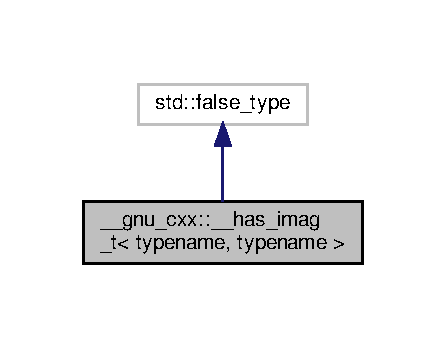
\includegraphics[width=214pt]{struct____gnu__cxx_1_1____has__imag__t__inherit__graph}
\end{center}
\end{figure}


Collaboration diagram for \+\_\+\+\_\+gnu\+\_\+cxx\+:\+:\+\_\+\+\_\+has\+\_\+imag\+\_\+t$<$ typename, typename $>$\+:
\nopagebreak
\begin{figure}[H]
\begin{center}
\leavevmode
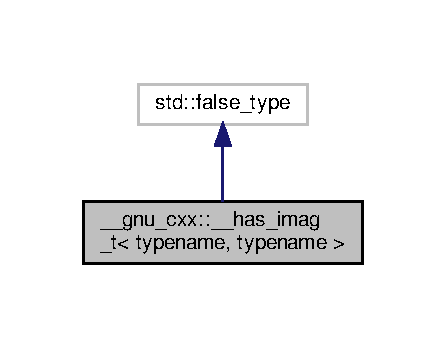
\includegraphics[width=214pt]{struct____gnu__cxx_1_1____has__imag__t__coll__graph}
\end{center}
\end{figure}


\subsection{Detailed Description}
\subsubsection*{template$<$typename, typename = std\+::void\+\_\+t$<$$>$$>$\newline
struct \+\_\+\+\_\+gnu\+\_\+cxx\+::\+\_\+\+\_\+has\+\_\+imag\+\_\+t$<$ typename, typename $>$}



Definition at line 94 of file polynomial.\+h.



The documentation for this struct was generated from the following file\+:\begin{DoxyCompactItemize}
\item 
include/ext/\hyperlink{polynomial_8h}{polynomial.\+h}\end{DoxyCompactItemize}

\hypertarget{struct____gnu__cxx_1_1____has__imag__t_3_01T_00_01std_1_1void__t_3_01decltype_07std_1_1declval_389ee8aaba7dec2e199e7ad81d6cda763}{}\section{\+\_\+\+\_\+gnu\+\_\+cxx\+:\+:\+\_\+\+\_\+has\+\_\+imag\+\_\+t$<$ T, std\+:\+:void\+\_\+t$<$ decltype(std\+:\+:declval$<$ T \& $>$().imag())$>$ $>$ Struct Template Reference}
\label{struct____gnu__cxx_1_1____has__imag__t_3_01T_00_01std_1_1void__t_3_01decltype_07std_1_1declval_389ee8aaba7dec2e199e7ad81d6cda763}\index{\+\_\+\+\_\+gnu\+\_\+cxx\+::\+\_\+\+\_\+has\+\_\+imag\+\_\+t$<$ T, std\+::void\+\_\+t$<$ decltype(std\+::declval$<$ T \& $>$().\+imag())$>$ $>$@{\+\_\+\+\_\+gnu\+\_\+cxx\+::\+\_\+\+\_\+has\+\_\+imag\+\_\+t$<$ T, std\+::void\+\_\+t$<$ decltype(std\+::declval$<$ T \& $>$().\+imag())$>$ $>$}}


{\ttfamily \#include $<$polynomial.\+h$>$}



Inheritance diagram for \+\_\+\+\_\+gnu\+\_\+cxx\+:\+:\+\_\+\+\_\+has\+\_\+imag\+\_\+t$<$ T, std\+:\+:void\+\_\+t$<$ decltype(std\+:\+:declval$<$ T \& $>$().imag())$>$ $>$\+:
\nopagebreak
\begin{figure}[H]
\begin{center}
\leavevmode
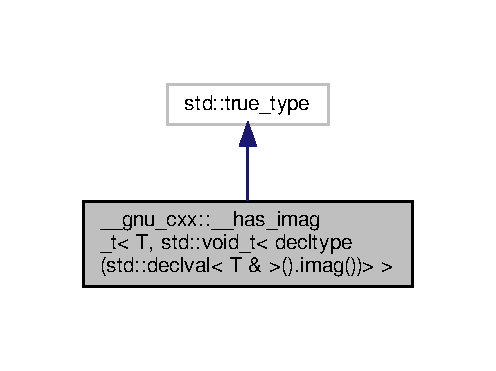
\includegraphics[width=238pt]{struct____gnu__cxx_1_1____has__imag__t_3_01T_00_01std_1_1void__t_3_01decltype_07std_1_1declval_3f9e8e0da80d34a132b8da0cdc144eae1}
\end{center}
\end{figure}


Collaboration diagram for \+\_\+\+\_\+gnu\+\_\+cxx\+:\+:\+\_\+\+\_\+has\+\_\+imag\+\_\+t$<$ T, std\+:\+:void\+\_\+t$<$ decltype(std\+:\+:declval$<$ T \& $>$().imag())$>$ $>$\+:
\nopagebreak
\begin{figure}[H]
\begin{center}
\leavevmode
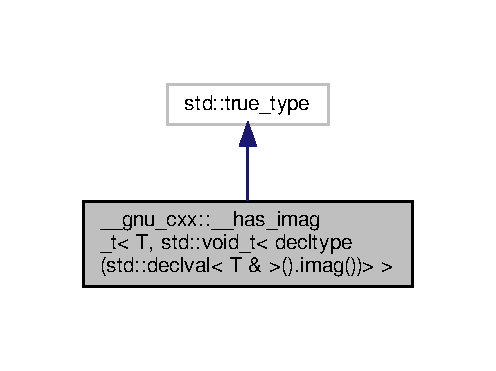
\includegraphics[width=238pt]{struct____gnu__cxx_1_1____has__imag__t_3_01T_00_01std_1_1void__t_3_01decltype_07std_1_1declval_3cb6c63a7804d363515b69cb8f2b24389}
\end{center}
\end{figure}


\subsection{Detailed Description}
\subsubsection*{template$<$typename T$>$\newline
struct \+\_\+\+\_\+gnu\+\_\+cxx\+::\+\_\+\+\_\+has\+\_\+imag\+\_\+t$<$ T, std\+::void\+\_\+t$<$ decltype(std\+::declval$<$ T \& $>$().\+imag())$>$ $>$}



Definition at line 99 of file polynomial.\+h.



The documentation for this struct was generated from the following file\+:\begin{DoxyCompactItemize}
\item 
include/ext/\hyperlink{polynomial_8h}{polynomial.\+h}\end{DoxyCompactItemize}

\hypertarget{class____gnu__cxx_1_1__Polynomial}{}\section{\+\_\+\+\_\+gnu\+\_\+cxx\+:\+:\+\_\+\+Polynomial$<$ \+\_\+\+Tp $>$ Class Template Reference}
\label{class____gnu__cxx_1_1__Polynomial}\index{\+\_\+\+\_\+gnu\+\_\+cxx\+::\+\_\+\+Polynomial$<$ \+\_\+\+Tp $>$@{\+\_\+\+\_\+gnu\+\_\+cxx\+::\+\_\+\+Polynomial$<$ \+\_\+\+Tp $>$}}


A dense polynomial class with a contiguous array of coefficients. The coefficients are lowest-\/order first\+: \[ P(x) = a_0 + a_1 x + ... + a_n x^n \].  




{\ttfamily \#include $<$polynomial.\+h$>$}

\subsection*{Public Types}
\begin{DoxyCompactItemize}
\item 
using \hyperlink{class____gnu__cxx_1_1__Polynomial_a96e4523cc2a834724fe4224f0800486b}{const\+\_\+iterator} = typename std\+::vector$<$ \hyperlink{class____gnu__cxx_1_1__Polynomial_a725563351f50e76084a7a016c06f8a53}{value\+\_\+type} $>$\+::\hyperlink{class____gnu__cxx_1_1__Polynomial_a96e4523cc2a834724fe4224f0800486b}{const\+\_\+iterator}
\item 
using \hyperlink{class____gnu__cxx_1_1__Polynomial_aaf4c4bbd516b837df5fe70b3bda4e9af}{const\+\_\+pointer} = typename std\+::vector$<$ \hyperlink{class____gnu__cxx_1_1__Polynomial_a725563351f50e76084a7a016c06f8a53}{value\+\_\+type} $>$\+::\hyperlink{class____gnu__cxx_1_1__Polynomial_aaf4c4bbd516b837df5fe70b3bda4e9af}{const\+\_\+pointer}
\item 
using \hyperlink{class____gnu__cxx_1_1__Polynomial_a55e17774f3387e74adb57376d099cf16}{const\+\_\+reference} = typename std\+::vector$<$ \hyperlink{class____gnu__cxx_1_1__Polynomial_a725563351f50e76084a7a016c06f8a53}{value\+\_\+type} $>$\+::\hyperlink{class____gnu__cxx_1_1__Polynomial_a55e17774f3387e74adb57376d099cf16}{const\+\_\+reference}
\item 
using \hyperlink{class____gnu__cxx_1_1__Polynomial_a2a042a80127ab9a7b0349a54791e59af}{const\+\_\+reverse\+\_\+iterator} = typename std\+::vector$<$ \hyperlink{class____gnu__cxx_1_1__Polynomial_a725563351f50e76084a7a016c06f8a53}{value\+\_\+type} $>$\+::\hyperlink{class____gnu__cxx_1_1__Polynomial_a2a042a80127ab9a7b0349a54791e59af}{const\+\_\+reverse\+\_\+iterator}
\item 
using \hyperlink{class____gnu__cxx_1_1__Polynomial_aefb6d7ae1935b99a332d5b96b1e82d32}{difference\+\_\+type} = typename std\+::vector$<$ \+\_\+\+Tp $>$\+::\hyperlink{class____gnu__cxx_1_1__Polynomial_aefb6d7ae1935b99a332d5b96b1e82d32}{difference\+\_\+type}
\item 
using \hyperlink{class____gnu__cxx_1_1__Polynomial_a64bd557b6af46992e352dbe9e30fa201}{iterator} = typename std\+::vector$<$ \hyperlink{class____gnu__cxx_1_1__Polynomial_a725563351f50e76084a7a016c06f8a53}{value\+\_\+type} $>$\+::\hyperlink{class____gnu__cxx_1_1__Polynomial_a64bd557b6af46992e352dbe9e30fa201}{iterator}
\item 
using \hyperlink{class____gnu__cxx_1_1__Polynomial_a876dcb9c1b92c4896a3f3b9f26e7e3df}{pointer} = typename std\+::vector$<$ \hyperlink{class____gnu__cxx_1_1__Polynomial_a725563351f50e76084a7a016c06f8a53}{value\+\_\+type} $>$\+::\hyperlink{class____gnu__cxx_1_1__Polynomial_a876dcb9c1b92c4896a3f3b9f26e7e3df}{pointer}
\item 
using \hyperlink{class____gnu__cxx_1_1__Polynomial_accb3b4df60e4ad82d466173d54ea731a}{reference} = typename std\+::vector$<$ \hyperlink{class____gnu__cxx_1_1__Polynomial_a725563351f50e76084a7a016c06f8a53}{value\+\_\+type} $>$\+::\hyperlink{class____gnu__cxx_1_1__Polynomial_accb3b4df60e4ad82d466173d54ea731a}{reference}
\item 
using \hyperlink{class____gnu__cxx_1_1__Polynomial_aed8f7d97c575d5c34c54170631953415}{reverse\+\_\+iterator} = typename std\+::vector$<$ \hyperlink{class____gnu__cxx_1_1__Polynomial_a725563351f50e76084a7a016c06f8a53}{value\+\_\+type} $>$\+::\hyperlink{class____gnu__cxx_1_1__Polynomial_aed8f7d97c575d5c34c54170631953415}{reverse\+\_\+iterator}
\item 
using \hyperlink{class____gnu__cxx_1_1__Polynomial_a6afe219c123c7a2fdc5abac8a6639053}{size\+\_\+type} = typename std\+::vector$<$ \+\_\+\+Tp $>$\+::\hyperlink{class____gnu__cxx_1_1__Polynomial_a6afe219c123c7a2fdc5abac8a6639053}{size\+\_\+type}
\item 
using \hyperlink{class____gnu__cxx_1_1__Polynomial_a725563351f50e76084a7a016c06f8a53}{value\+\_\+type} = typename std\+::vector$<$ \+\_\+\+Tp $>$\+::\hyperlink{class____gnu__cxx_1_1__Polynomial_a725563351f50e76084a7a016c06f8a53}{value\+\_\+type}
\end{DoxyCompactItemize}
\subsection*{Public Member Functions}
\begin{DoxyCompactItemize}
\item 
\hyperlink{class____gnu__cxx_1_1__Polynomial_ad2baf4c12b7e3ab131a592afa3f391ae}{\+\_\+\+Polynomial} ()
\item 
\hyperlink{class____gnu__cxx_1_1__Polynomial_ac0a657bc804f3db8a03acfd1b98abb39}{\+\_\+\+Polynomial} (const \hyperlink{class____gnu__cxx_1_1__Polynomial}{\+\_\+\+Polynomial} \&)=default
\item 
\hyperlink{class____gnu__cxx_1_1__Polynomial_a87bad90934c9752b51cdece15a5b369f}{\+\_\+\+Polynomial} (\hyperlink{class____gnu__cxx_1_1__Polynomial}{\+\_\+\+Polynomial} \&\&) noexcept=default
\item 
{\footnotesize template$<$typename \+\_\+\+Up $>$ }\\\hyperlink{class____gnu__cxx_1_1__Polynomial_ae744374b972b91a9609ba6cc1330bbfd}{\+\_\+\+Polynomial} (const \hyperlink{class____gnu__cxx_1_1__Polynomial}{\+\_\+\+Polynomial}$<$ \hyperlink{class____gnu__cxx_1_1__Polynomial_a242114d4b86648a5dff67a8221f80d40}{\+\_\+\+Up} $>$ \&\+\_\+\+\_\+poly)
\item 
\hyperlink{class____gnu__cxx_1_1__Polynomial_ad89b416fedd4e3a23b484d5269767a93}{\+\_\+\+Polynomial} (\hyperlink{class____gnu__cxx_1_1__Polynomial_a725563351f50e76084a7a016c06f8a53}{value\+\_\+type} \+\_\+\+\_\+a, \hyperlink{class____gnu__cxx_1_1__Polynomial_a6afe219c123c7a2fdc5abac8a6639053}{size\+\_\+type} \+\_\+\+\_\+degree=0)
\item 
\hyperlink{class____gnu__cxx_1_1__Polynomial_acc6b7b2a52600f62bf8dee99f2fb787c}{\+\_\+\+Polynomial} (std\+::initializer\+\_\+list$<$ \hyperlink{class____gnu__cxx_1_1__Polynomial_a725563351f50e76084a7a016c06f8a53}{value\+\_\+type} $>$ \+\_\+\+\_\+ila)
\item 
{\footnotesize template$<$typename In\+Iter , typename  = std\+::\+\_\+\+Require\+Input\+Iter$<$\+In\+Iter$>$$>$ }\\\hyperlink{class____gnu__cxx_1_1__Polynomial_a45589d1d036861179488c44f3029f335}{\+\_\+\+Polynomial} (const In\+Iter \&\+\_\+\+\_\+abegin, const In\+Iter \&\+\_\+\+\_\+aend)
\item 
{\footnotesize template$<$typename In\+Iter , typename  = std\+::\+\_\+\+Require\+Input\+Iter$<$\+In\+Iter$>$$>$ }\\\hyperlink{class____gnu__cxx_1_1__Polynomial_a86249f53e97e72eff11242a8ba85ba4c}{\+\_\+\+Polynomial} (const In\+Iter \&\+\_\+\+\_\+xbegin, const In\+Iter \&\+\_\+\+\_\+xend, const In\+Iter \&\+\_\+\+\_\+ybegin)
\item 
{\footnotesize template$<$typename Gen $>$ }\\\hyperlink{class____gnu__cxx_1_1__Polynomial_ad6e0daed9aa3a89cd98441a0fc4fa9f1}{\+\_\+\+Polynomial} (Gen \+\_\+\+\_\+gen, \hyperlink{class____gnu__cxx_1_1__Polynomial_a6afe219c123c7a2fdc5abac8a6639053}{size\+\_\+type} \+\_\+\+\_\+degree)
\item 
\hyperlink{class____gnu__cxx_1_1__Polynomial_a64bd557b6af46992e352dbe9e30fa201}{iterator} \hyperlink{class____gnu__cxx_1_1__Polynomial_a2f9cf484724c2aef472975fc3d8bd99d}{begin} () noexcept
\item 
\hyperlink{class____gnu__cxx_1_1__Polynomial_a96e4523cc2a834724fe4224f0800486b}{const\+\_\+iterator} \hyperlink{class____gnu__cxx_1_1__Polynomial_a57902287656245f5ae1ee7406b419c9b}{begin} () const noexcept
\item 
\hyperlink{class____gnu__cxx_1_1__Polynomial_a96e4523cc2a834724fe4224f0800486b}{const\+\_\+iterator} \hyperlink{class____gnu__cxx_1_1__Polynomial_a3309265141727a7581036a2b7632c689}{cbegin} () const noexcept
\item 
\hyperlink{class____gnu__cxx_1_1__Polynomial_a96e4523cc2a834724fe4224f0800486b}{const\+\_\+iterator} \hyperlink{class____gnu__cxx_1_1__Polynomial_ae3d5b393866c55f9585a1e0e10c41cc4}{cend} () const noexcept
\item 
\hyperlink{class____gnu__cxx_1_1__Polynomial_a725563351f50e76084a7a016c06f8a53}{value\+\_\+type} \hyperlink{class____gnu__cxx_1_1__Polynomial_a7cee31b3acbe8c024af6d696bc610f49}{coefficient} (\hyperlink{class____gnu__cxx_1_1__Polynomial_a6afe219c123c7a2fdc5abac8a6639053}{size\+\_\+type} \+\_\+\+\_\+i) const
\item 
void \hyperlink{class____gnu__cxx_1_1__Polynomial_a191611909a0461c449984a0898bce38f}{coefficient} (\hyperlink{class____gnu__cxx_1_1__Polynomial_a6afe219c123c7a2fdc5abac8a6639053}{size\+\_\+type} \+\_\+\+\_\+i, \hyperlink{class____gnu__cxx_1_1__Polynomial_a725563351f50e76084a7a016c06f8a53}{value\+\_\+type} \+\_\+\+\_\+val)
\item 
const \hyperlink{class____gnu__cxx_1_1__Polynomial_a725563351f50e76084a7a016c06f8a53}{value\+\_\+type} $\ast$ \hyperlink{class____gnu__cxx_1_1__Polynomial_a19a59153698d550a7473860bb8cadb6f}{coefficients} () const noexcept
\item 
\hyperlink{class____gnu__cxx_1_1__Polynomial_a725563351f50e76084a7a016c06f8a53}{value\+\_\+type} $\ast$ \hyperlink{class____gnu__cxx_1_1__Polynomial_ace23c82d514bb2b7b4e79494bcc47ea7}{coefficients} () noexcept
\item 
\hyperlink{class____gnu__cxx_1_1__Polynomial_a2a042a80127ab9a7b0349a54791e59af}{const\+\_\+reverse\+\_\+iterator} \hyperlink{class____gnu__cxx_1_1__Polynomial_a263b74157472085ae2fb01957a5bda5e}{crbegin} () const noexcept
\item 
\hyperlink{class____gnu__cxx_1_1__Polynomial_a2a042a80127ab9a7b0349a54791e59af}{const\+\_\+reverse\+\_\+iterator} \hyperlink{class____gnu__cxx_1_1__Polynomial_a0b314ced62a607798572646a76f2ac35}{crend} () const noexcept
\item 
\hyperlink{class____gnu__cxx_1_1__Polynomial_a6afe219c123c7a2fdc5abac8a6639053}{size\+\_\+type} \hyperlink{class____gnu__cxx_1_1__Polynomial_a07d9933aeeb9afbd823218ed921336cb}{degree} () const noexcept
\item 
void \hyperlink{class____gnu__cxx_1_1__Polynomial_af6ae7990b6185dc3597a8a5d6abdd13a}{degree} (\hyperlink{class____gnu__cxx_1_1__Polynomial_a6afe219c123c7a2fdc5abac8a6639053}{size\+\_\+type} \+\_\+\+\_\+degree)
\item 
\hyperlink{class____gnu__cxx_1_1__Polynomial}{\+\_\+\+Polynomial} \hyperlink{class____gnu__cxx_1_1__Polynomial_a69e973ccaf5857251a8b7971e19a5ec7}{derivative} () const
\item 
\hyperlink{class____gnu__cxx_1_1__Polynomial_a64bd557b6af46992e352dbe9e30fa201}{iterator} \hyperlink{class____gnu__cxx_1_1__Polynomial_a7997059cf934fc454497be9074ebc958}{end} () noexcept
\item 
\hyperlink{class____gnu__cxx_1_1__Polynomial_a96e4523cc2a834724fe4224f0800486b}{const\+\_\+iterator} \hyperlink{class____gnu__cxx_1_1__Polynomial_a3f971eb02150e9ca66e8222ba4a5aa3d}{end} () const noexcept
\item 
{\footnotesize template$<$typename \+\_\+\+Polynomial$<$ \+\_\+\+Tp $>$\+::size\+\_\+type N$>$ }\\void \hyperlink{class____gnu__cxx_1_1__Polynomial_a5558b16a9a4b594e506d30e5d10289b4}{eval} (typename \hyperlink{class____gnu__cxx_1_1__Polynomial}{\+\_\+\+Polynomial}$<$ \+\_\+\+Tp $>$\+::\hyperlink{class____gnu__cxx_1_1__Polynomial_a725563351f50e76084a7a016c06f8a53}{value\+\_\+type} \+\_\+\+\_\+x, std\+::array$<$ \hyperlink{class____gnu__cxx_1_1__Polynomial}{\+\_\+\+Polynomial}$<$ \+\_\+\+Tp $>$\+::\hyperlink{class____gnu__cxx_1_1__Polynomial_a725563351f50e76084a7a016c06f8a53}{value\+\_\+type}, N $>$ \&\+\_\+\+\_\+arr)
\item 
{\footnotesize template$<$typename Out\+Iter$>$ }\\void \hyperlink{class____gnu__cxx_1_1__Polynomial_a2251cb8f6518118c78494f4eb015ed8f}{eval} (typename \hyperlink{class____gnu__cxx_1_1__Polynomial}{\+\_\+\+Polynomial}$<$ \+\_\+\+Tp $>$\+::\hyperlink{class____gnu__cxx_1_1__Polynomial_a725563351f50e76084a7a016c06f8a53}{value\+\_\+type} \+\_\+\+\_\+x, Out\+Iter \+\_\+\+\_\+b, Out\+Iter \+\_\+\+\_\+e)
\item 
{\footnotesize template$<$size\+\_\+type N$>$ }\\void \hyperlink{class____gnu__cxx_1_1__Polynomial_a3c3b539828301eef5385bc5b230a844a}{eval} (\hyperlink{class____gnu__cxx_1_1__Polynomial_a725563351f50e76084a7a016c06f8a53}{value\+\_\+type} \+\_\+\+\_\+x, std\+::array$<$ \hyperlink{class____gnu__cxx_1_1__Polynomial_a725563351f50e76084a7a016c06f8a53}{value\+\_\+type}, N $>$ \&\+\_\+\+\_\+arr)
\item 
{\footnotesize template$<$typename Out\+Iter $>$ }\\void \hyperlink{class____gnu__cxx_1_1__Polynomial_a409ca632845c145fcf08f8c3e8eeae63}{eval} (\hyperlink{class____gnu__cxx_1_1__Polynomial_a725563351f50e76084a7a016c06f8a53}{value\+\_\+type} \+\_\+\+\_\+x, Out\+Iter \+\_\+\+\_\+b, Out\+Iter \+\_\+\+\_\+e)
\item 
{\footnotesize template$<$typename \+\_\+\+Tp $>$ }\\\hyperlink{class____gnu__cxx_1_1__Polynomial}{\+\_\+\+Polynomial}$<$ \+\_\+\+Tp $>$\+::\hyperlink{class____gnu__cxx_1_1__Polynomial_a725563351f50e76084a7a016c06f8a53}{value\+\_\+type} \hyperlink{class____gnu__cxx_1_1__Polynomial_a5e3d2496522f241c6fae41d222819a59}{eval\+\_\+even} (typename \hyperlink{class____gnu__cxx_1_1__Polynomial}{\+\_\+\+Polynomial}$<$ \+\_\+\+Tp $>$\+::\hyperlink{class____gnu__cxx_1_1__Polynomial_a725563351f50e76084a7a016c06f8a53}{value\+\_\+type} \+\_\+\+\_\+x) const
\item 
\hyperlink{class____gnu__cxx_1_1__Polynomial_a725563351f50e76084a7a016c06f8a53}{value\+\_\+type} \hyperlink{class____gnu__cxx_1_1__Polynomial_ac70ecc3968e15077ef2d68390d150f5a}{eval\+\_\+even} (\hyperlink{class____gnu__cxx_1_1__Polynomial_a725563351f50e76084a7a016c06f8a53}{value\+\_\+type} \+\_\+\+\_\+x) const
\item 
{\footnotesize template$<$typename \+\_\+\+Up $>$ }\\auto \hyperlink{class____gnu__cxx_1_1__Polynomial_a7314653c50b311781a26ac74789d84a1}{eval\+\_\+even} (const \hyperlink{classstd_1_1complex}{std\+::complex}$<$ \hyperlink{class____gnu__cxx_1_1__Polynomial_a242114d4b86648a5dff67a8221f80d40}{\+\_\+\+Up} $>$ \&\+\_\+\+\_\+z) const -\/$>$ std\+::enable\+\_\+if\+\_\+t$<$!\hyperlink{namespace____gnu__cxx_afa2404a914b06f950f3a46e75aca51a9}{\+\_\+\+\_\+has\+\_\+imag\+\_\+v}$<$ \+\_\+\+Tp $>$, \hyperlink{classstd_1_1complex}{std\+::complex}$<$ std\+::decay\+\_\+t$<$ decltype(typename \hyperlink{class____gnu__cxx_1_1__Polynomial}{\+\_\+\+Polynomial}$<$ \+\_\+\+Tp $>$\+::\hyperlink{class____gnu__cxx_1_1__Polynomial_a725563351f50e76084a7a016c06f8a53}{value\+\_\+type}
\item 
{\footnotesize template$<$typename \+\_\+\+Tp $>$ }\\\hyperlink{class____gnu__cxx_1_1__Polynomial}{\+\_\+\+Polynomial}$<$ \+\_\+\+Tp $>$\+::\hyperlink{class____gnu__cxx_1_1__Polynomial_a725563351f50e76084a7a016c06f8a53}{value\+\_\+type} \hyperlink{class____gnu__cxx_1_1__Polynomial_acd4fd2288b7dd7a5933e84ae372d4769}{eval\+\_\+odd} (typename \hyperlink{class____gnu__cxx_1_1__Polynomial}{\+\_\+\+Polynomial}$<$ \+\_\+\+Tp $>$\+::\hyperlink{class____gnu__cxx_1_1__Polynomial_a725563351f50e76084a7a016c06f8a53}{value\+\_\+type} \+\_\+\+\_\+x) const
\item 
\hyperlink{class____gnu__cxx_1_1__Polynomial_a725563351f50e76084a7a016c06f8a53}{value\+\_\+type} \hyperlink{class____gnu__cxx_1_1__Polynomial_aff02472cad1aa3b6c8d067fdd4b11bc0}{eval\+\_\+odd} (\hyperlink{class____gnu__cxx_1_1__Polynomial_a725563351f50e76084a7a016c06f8a53}{value\+\_\+type} \+\_\+\+\_\+x) const
\item 
{\footnotesize template$<$typename \+\_\+\+Up $>$ }\\auto \hyperlink{class____gnu__cxx_1_1__Polynomial_a5348bf4c4db826660a133ab731f775c1}{eval\+\_\+odd} (const \hyperlink{classstd_1_1complex}{std\+::complex}$<$ \hyperlink{class____gnu__cxx_1_1__Polynomial_a242114d4b86648a5dff67a8221f80d40}{\+\_\+\+Up} $>$ \&\+\_\+\+\_\+z) const -\/$>$ std\+::enable\+\_\+if\+\_\+t$<$!\hyperlink{namespace____gnu__cxx_afa2404a914b06f950f3a46e75aca51a9}{\+\_\+\+\_\+has\+\_\+imag\+\_\+v}$<$ \+\_\+\+Tp $>$, \hyperlink{classstd_1_1complex}{std\+::complex}$<$ std\+::decay\+\_\+t$<$ decltype(typename \hyperlink{class____gnu__cxx_1_1__Polynomial}{\+\_\+\+Polynomial}$<$ \+\_\+\+Tp $>$\+::\hyperlink{class____gnu__cxx_1_1__Polynomial_a725563351f50e76084a7a016c06f8a53}{value\+\_\+type}
\item 
\hyperlink{class____gnu__cxx_1_1__Polynomial}{\+\_\+\+Polynomial} \hyperlink{class____gnu__cxx_1_1__Polynomial_a4f9871fb66fc6075767f1db61a323fd0}{integral} (\hyperlink{class____gnu__cxx_1_1__Polynomial_a725563351f50e76084a7a016c06f8a53}{value\+\_\+type} \+\_\+\+\_\+c=\hyperlink{class____gnu__cxx_1_1__Polynomial_a725563351f50e76084a7a016c06f8a53}{value\+\_\+type}\{\}) const
\item 
{\footnotesize template$<$typename \+\_\+\+Up $>$ }\\\hyperlink{class____gnu__cxx_1_1__Polynomial}{\+\_\+\+Polynomial} \& \hyperlink{class____gnu__cxx_1_1__Polynomial_ade8196c94c8e169f00730730d0c6b99e}{operator\%=} (const \hyperlink{class____gnu__cxx_1_1__Polynomial_a242114d4b86648a5dff67a8221f80d40}{\+\_\+\+Up} \&)
\item 
{\footnotesize template$<$typename \+\_\+\+Up $>$ }\\\hyperlink{class____gnu__cxx_1_1__Polynomial}{\+\_\+\+Polynomial} \& \hyperlink{class____gnu__cxx_1_1__Polynomial_a66661e25c272a310f7bf1abbcc8fa2a9}{operator\%=} (const \hyperlink{class____gnu__cxx_1_1__Polynomial}{\+\_\+\+Polynomial}$<$ \hyperlink{class____gnu__cxx_1_1__Polynomial_a242114d4b86648a5dff67a8221f80d40}{\+\_\+\+Up} $>$ \&\+\_\+\+\_\+poly)
\item 
{\footnotesize template$<$typename \+\_\+\+Up $>$ }\\auto \hyperlink{class____gnu__cxx_1_1__Polynomial_a14a9a08043909e50269eef0d66995794}{operator()} (const \hyperlink{classstd_1_1complex}{std\+::complex}$<$ \hyperlink{class____gnu__cxx_1_1__Polynomial_a242114d4b86648a5dff67a8221f80d40}{\+\_\+\+Up} $>$ \&\+\_\+\+\_\+z) const -\/$>$ decltype(\hyperlink{class____gnu__cxx_1_1__Polynomial}{\+\_\+\+Polynomial}$<$ \+\_\+\+Tp $>$\+::\hyperlink{class____gnu__cxx_1_1__Polynomial_a725563351f50e76084a7a016c06f8a53}{value\+\_\+type}
\item 
\hyperlink{class____gnu__cxx_1_1__Polynomial_a725563351f50e76084a7a016c06f8a53}{value\+\_\+type} \hyperlink{class____gnu__cxx_1_1__Polynomial_a9aa91f3424896c07d51fa09950825549}{operator()} (\hyperlink{class____gnu__cxx_1_1__Polynomial_a725563351f50e76084a7a016c06f8a53}{value\+\_\+type} \+\_\+\+\_\+x) const
\item 
{\footnotesize template$<$typename \+\_\+\+Up $>$ }\\auto \hyperlink{class____gnu__cxx_1_1__Polynomial_a064c220c67f2d72104b3d4767ca5cc42}{operator()} (\hyperlink{class____gnu__cxx_1_1__Polynomial_a242114d4b86648a5dff67a8221f80d40}{\+\_\+\+Up} \+\_\+\+\_\+x) const -\/$>$ decltype(\hyperlink{class____gnu__cxx_1_1__Polynomial_a725563351f50e76084a7a016c06f8a53}{value\+\_\+type}
\item 
{\footnotesize template$<$typename In\+Iter , typename Out\+Iter , typename  = std\+::\+\_\+\+Require\+Input\+Iter$<$\+In\+Iter$>$$>$ }\\Out\+Iter \hyperlink{class____gnu__cxx_1_1__Polynomial_a06d7b0b57d6764da29049b3c2b6f890c}{operator()} (const In\+Iter \&\+\_\+\+\_\+xbegin, const In\+Iter \&\+\_\+\+\_\+xend, Out\+Iter \&\+\_\+\+\_\+pbegin) const
\item 
{\footnotesize template$<$typename \+\_\+\+Up $>$ }\\\hyperlink{class____gnu__cxx_1_1__Polynomial}{\+\_\+\+Polynomial}$<$ \+\_\+\+Tp $>$ \& \hyperlink{class____gnu__cxx_1_1__Polynomial_a5e5dae4944bc0352b6b360f8decd2d07}{operator$\ast$=} (const \hyperlink{class____gnu__cxx_1_1__Polynomial}{\+\_\+\+Polynomial}$<$ \hyperlink{class____gnu__cxx_1_1__Polynomial_a242114d4b86648a5dff67a8221f80d40}{\+\_\+\+Up} $>$ \&\+\_\+\+\_\+poly)
\item 
{\footnotesize template$<$typename \+\_\+\+Up $>$ }\\\hyperlink{class____gnu__cxx_1_1__Polynomial}{\+\_\+\+Polynomial} \& \hyperlink{class____gnu__cxx_1_1__Polynomial_ad5b3128a53c12abe9147832a1a581f6a}{operator$\ast$=} (const \hyperlink{class____gnu__cxx_1_1__Polynomial_a242114d4b86648a5dff67a8221f80d40}{\+\_\+\+Up} \&\+\_\+\+\_\+x)
\item 
{\footnotesize template$<$typename \+\_\+\+Up $>$ }\\\hyperlink{class____gnu__cxx_1_1__Polynomial}{\+\_\+\+Polynomial} \& \hyperlink{class____gnu__cxx_1_1__Polynomial_ab7daa447472ac775ee38ef0db323bb19}{operator$\ast$=} (const \hyperlink{class____gnu__cxx_1_1__Polynomial}{\+\_\+\+Polynomial}$<$ \hyperlink{class____gnu__cxx_1_1__Polynomial_a242114d4b86648a5dff67a8221f80d40}{\+\_\+\+Up} $>$ \&\+\_\+\+\_\+poly)
\item 
\hyperlink{class____gnu__cxx_1_1__Polynomial}{\+\_\+\+Polynomial} \hyperlink{class____gnu__cxx_1_1__Polynomial_acbaf9cbeb167e41490d976a083f131d8}{operator+} () const noexcept
\item 
{\footnotesize template$<$typename \+\_\+\+Up $>$ }\\\hyperlink{class____gnu__cxx_1_1__Polynomial}{\+\_\+\+Polynomial} \& \hyperlink{class____gnu__cxx_1_1__Polynomial_a68658f4f4692cd8a840919123d03995a}{operator+=} (const \hyperlink{class____gnu__cxx_1_1__Polynomial_a242114d4b86648a5dff67a8221f80d40}{\+\_\+\+Up} \&\+\_\+\+\_\+x)
\item 
{\footnotesize template$<$typename \+\_\+\+Up $>$ }\\\hyperlink{class____gnu__cxx_1_1__Polynomial}{\+\_\+\+Polynomial} \& \hyperlink{class____gnu__cxx_1_1__Polynomial_ac7b0aafe9829a3eae65f79a99881fac2}{operator+=} (const \hyperlink{class____gnu__cxx_1_1__Polynomial}{\+\_\+\+Polynomial}$<$ \hyperlink{class____gnu__cxx_1_1__Polynomial_a242114d4b86648a5dff67a8221f80d40}{\+\_\+\+Up} $>$ \&\+\_\+\+\_\+poly)
\item 
\hyperlink{class____gnu__cxx_1_1__Polynomial}{\+\_\+\+Polynomial} \hyperlink{class____gnu__cxx_1_1__Polynomial_a814ac6ceea7d2b6d42c371b4d631b47f}{operator-\/} () const
\item 
{\footnotesize template$<$typename \+\_\+\+Up $>$ }\\\hyperlink{class____gnu__cxx_1_1__Polynomial}{\+\_\+\+Polynomial} \& \hyperlink{class____gnu__cxx_1_1__Polynomial_a4fa6ae9adb4c4f946839d29b033ededb}{operator-\/=} (const \hyperlink{class____gnu__cxx_1_1__Polynomial_a242114d4b86648a5dff67a8221f80d40}{\+\_\+\+Up} \&\+\_\+\+\_\+x)
\item 
{\footnotesize template$<$typename \+\_\+\+Up $>$ }\\\hyperlink{class____gnu__cxx_1_1__Polynomial}{\+\_\+\+Polynomial} \& \hyperlink{class____gnu__cxx_1_1__Polynomial_af092dce5f209610ec20ea84ccfe0a5f1}{operator-\/=} (const \hyperlink{class____gnu__cxx_1_1__Polynomial}{\+\_\+\+Polynomial}$<$ \hyperlink{class____gnu__cxx_1_1__Polynomial_a242114d4b86648a5dff67a8221f80d40}{\+\_\+\+Up} $>$ \&\+\_\+\+\_\+poly)
\item 
{\footnotesize template$<$typename \+\_\+\+Up $>$ }\\\hyperlink{class____gnu__cxx_1_1__Polynomial}{\+\_\+\+Polynomial} \& \hyperlink{class____gnu__cxx_1_1__Polynomial_a3fbb600980f4945af2733c9e10228079}{operator/=} (const \hyperlink{class____gnu__cxx_1_1__Polynomial_a242114d4b86648a5dff67a8221f80d40}{\+\_\+\+Up} \&\+\_\+\+\_\+x)
\item 
{\footnotesize template$<$typename \+\_\+\+Up $>$ }\\\hyperlink{class____gnu__cxx_1_1__Polynomial}{\+\_\+\+Polynomial} \& \hyperlink{class____gnu__cxx_1_1__Polynomial_a3374e3ab44ed1478de27f688aae6c3f1}{operator/=} (const \hyperlink{class____gnu__cxx_1_1__Polynomial}{\+\_\+\+Polynomial}$<$ \hyperlink{class____gnu__cxx_1_1__Polynomial_a242114d4b86648a5dff67a8221f80d40}{\+\_\+\+Up} $>$ \&\+\_\+\+\_\+poly)
\item 
\hyperlink{class____gnu__cxx_1_1__Polynomial}{\+\_\+\+Polynomial} \& \hyperlink{class____gnu__cxx_1_1__Polynomial_a207a09b3f170adcfbf21c26821c864dd}{operator=} (const \hyperlink{class____gnu__cxx_1_1__Polynomial_a725563351f50e76084a7a016c06f8a53}{value\+\_\+type} \&\+\_\+\+\_\+x)
\item 
\hyperlink{class____gnu__cxx_1_1__Polynomial}{\+\_\+\+Polynomial} \& \hyperlink{class____gnu__cxx_1_1__Polynomial_a96aa1f47da636376d63cf099558113b8}{operator=} (const \hyperlink{class____gnu__cxx_1_1__Polynomial}{\+\_\+\+Polynomial} \&)=default
\item 
{\footnotesize template$<$typename \+\_\+\+Up $>$ }\\\hyperlink{class____gnu__cxx_1_1__Polynomial}{\+\_\+\+Polynomial} \& \hyperlink{class____gnu__cxx_1_1__Polynomial_ab3287f4f0300adc76216e7fabeb62d7d}{operator=} (const \hyperlink{class____gnu__cxx_1_1__Polynomial}{\+\_\+\+Polynomial}$<$ \hyperlink{class____gnu__cxx_1_1__Polynomial_a242114d4b86648a5dff67a8221f80d40}{\+\_\+\+Up} $>$ \&\+\_\+\+\_\+poly)
\item 
\hyperlink{class____gnu__cxx_1_1__Polynomial}{\+\_\+\+Polynomial} \& \hyperlink{class____gnu__cxx_1_1__Polynomial_a44394532a2b1e67f1613b35402da9d47}{operator=} (std\+::initializer\+\_\+list$<$ \hyperlink{class____gnu__cxx_1_1__Polynomial_a725563351f50e76084a7a016c06f8a53}{value\+\_\+type} $>$ \+\_\+\+\_\+ila)
\item 
\hyperlink{class____gnu__cxx_1_1__Polynomial_a725563351f50e76084a7a016c06f8a53}{value\+\_\+type} \hyperlink{class____gnu__cxx_1_1__Polynomial_adda717f35cc87205daf0ea7a16d5d1a7}{operator\mbox{[}$\,$\mbox{]}} (\hyperlink{class____gnu__cxx_1_1__Polynomial_a6afe219c123c7a2fdc5abac8a6639053}{size\+\_\+type} \+\_\+\+\_\+i) const noexcept
\item 
\hyperlink{class____gnu__cxx_1_1__Polynomial_accb3b4df60e4ad82d466173d54ea731a}{reference} \hyperlink{class____gnu__cxx_1_1__Polynomial_a999ee3c5a82fe4b2fa39b7a237ff2cbf}{operator\mbox{[}$\,$\mbox{]}} (\hyperlink{class____gnu__cxx_1_1__Polynomial_a6afe219c123c7a2fdc5abac8a6639053}{size\+\_\+type} \+\_\+\+\_\+i) noexcept
\item 
\hyperlink{class____gnu__cxx_1_1__Polynomial_aed8f7d97c575d5c34c54170631953415}{reverse\+\_\+iterator} \hyperlink{class____gnu__cxx_1_1__Polynomial_a10924e0d5e228684c721a4bba73a7af3}{rbegin} () noexcept
\item 
\hyperlink{class____gnu__cxx_1_1__Polynomial_a2a042a80127ab9a7b0349a54791e59af}{const\+\_\+reverse\+\_\+iterator} \hyperlink{class____gnu__cxx_1_1__Polynomial_ab5cd3c6e861ebf3adac38e3df4e099aa}{rbegin} () const noexcept
\item 
\hyperlink{class____gnu__cxx_1_1__Polynomial_aed8f7d97c575d5c34c54170631953415}{reverse\+\_\+iterator} \hyperlink{class____gnu__cxx_1_1__Polynomial_a8373c6b9a787a52798e4319906858d33}{rend} () noexcept
\item 
\hyperlink{class____gnu__cxx_1_1__Polynomial_a2a042a80127ab9a7b0349a54791e59af}{const\+\_\+reverse\+\_\+iterator} \hyperlink{class____gnu__cxx_1_1__Polynomial_abeca4b1cffc4a52db34375b99b6d3d11}{rend} () const noexcept
\item 
\hyperlink{class____gnu__cxx_1_1__Polynomial_a6afe219c123c7a2fdc5abac8a6639053}{size\+\_\+type} \hyperlink{class____gnu__cxx_1_1__Polynomial_aa0ae73f79d58962dc4f1e4df2d2cc0d2}{size} () const noexcept
\item 
void \hyperlink{class____gnu__cxx_1_1__Polynomial_aec8b248101f7340d46fbac13b07b45bc}{swap} (\hyperlink{class____gnu__cxx_1_1__Polynomial}{\+\_\+\+Polynomial} \&\+\_\+\+\_\+poly) noexcept
\end{DoxyCompactItemize}
\subsection*{Public Attributes}
\begin{DoxyCompactItemize}
\item 
$\ast$ \hyperlink{class____gnu__cxx_1_1__Polynomial_a242114d4b86648a5dff67a8221f80d40}{\+\_\+\+Up}
\end{DoxyCompactItemize}
\subsection*{Friends}
\begin{DoxyCompactItemize}
\item 
{\footnotesize template$<$typename \+\_\+\+Tp1 $>$ }\\bool \hyperlink{class____gnu__cxx_1_1__Polynomial_abb21e2bfe0dc97a44ae9eeffb6f930aa}{operator==} (const \hyperlink{class____gnu__cxx_1_1__Polynomial}{\+\_\+\+Polynomial}$<$ \+\_\+\+Tp1 $>$ \&\+\_\+\+\_\+pa, const \hyperlink{class____gnu__cxx_1_1__Polynomial}{\+\_\+\+Polynomial}$<$ \+\_\+\+Tp1 $>$ \&\+\_\+\+\_\+pb)
\item 
{\footnotesize template$<$typename CharT , typename Traits , typename \+\_\+\+Tp1 $>$ }\\std\+::basic\+\_\+istream$<$ CharT, Traits $>$ \& \hyperlink{class____gnu__cxx_1_1__Polynomial_a929d1753cc00510f102f61a2bbeb0d2d}{operator$>$$>$} (std\+::basic\+\_\+istream$<$ CharT, Traits $>$ \&, \hyperlink{class____gnu__cxx_1_1__Polynomial}{\+\_\+\+Polynomial}$<$ \+\_\+\+Tp1 $>$ \&)
\end{DoxyCompactItemize}


\subsection{Detailed Description}
\subsubsection*{template$<$typename \+\_\+\+Tp$>$\newline
class \+\_\+\+\_\+gnu\+\_\+cxx\+::\+\_\+\+Polynomial$<$ \+\_\+\+Tp $>$}

A dense polynomial class with a contiguous array of coefficients. The coefficients are lowest-\/order first\+: \[ P(x) = a_0 + a_1 x + ... + a_n x^n \]. 

Definition at line 114 of file polynomial.\+h.



\subsection{Member Typedef Documentation}
\mbox{\Hypertarget{class____gnu__cxx_1_1__Polynomial_a96e4523cc2a834724fe4224f0800486b}\label{class____gnu__cxx_1_1__Polynomial_a96e4523cc2a834724fe4224f0800486b}} 
\index{\+\_\+\+\_\+gnu\+\_\+cxx\+::\+\_\+\+Polynomial@{\+\_\+\+\_\+gnu\+\_\+cxx\+::\+\_\+\+Polynomial}!const\+\_\+iterator@{const\+\_\+iterator}}
\index{const\+\_\+iterator@{const\+\_\+iterator}!\+\_\+\+\_\+gnu\+\_\+cxx\+::\+\_\+\+Polynomial@{\+\_\+\+\_\+gnu\+\_\+cxx\+::\+\_\+\+Polynomial}}
\subsubsection{\texorpdfstring{const\+\_\+iterator}{const\_iterator}}
{\footnotesize\ttfamily template$<$typename \+\_\+\+Tp$>$ \\
using \hyperlink{class____gnu__cxx_1_1__Polynomial}{\+\_\+\+\_\+gnu\+\_\+cxx\+::\+\_\+\+Polynomial}$<$ \+\_\+\+Tp $>$\+::\hyperlink{class____gnu__cxx_1_1__Polynomial_a96e4523cc2a834724fe4224f0800486b}{const\+\_\+iterator} =  typename std\+::vector$<$\hyperlink{class____gnu__cxx_1_1__Polynomial_a725563351f50e76084a7a016c06f8a53}{value\+\_\+type}$>$\+::\hyperlink{class____gnu__cxx_1_1__Polynomial_a96e4523cc2a834724fe4224f0800486b}{const\+\_\+iterator}}



Definition at line 126 of file polynomial.\+h.

\mbox{\Hypertarget{class____gnu__cxx_1_1__Polynomial_aaf4c4bbd516b837df5fe70b3bda4e9af}\label{class____gnu__cxx_1_1__Polynomial_aaf4c4bbd516b837df5fe70b3bda4e9af}} 
\index{\+\_\+\+\_\+gnu\+\_\+cxx\+::\+\_\+\+Polynomial@{\+\_\+\+\_\+gnu\+\_\+cxx\+::\+\_\+\+Polynomial}!const\+\_\+pointer@{const\+\_\+pointer}}
\index{const\+\_\+pointer@{const\+\_\+pointer}!\+\_\+\+\_\+gnu\+\_\+cxx\+::\+\_\+\+Polynomial@{\+\_\+\+\_\+gnu\+\_\+cxx\+::\+\_\+\+Polynomial}}
\subsubsection{\texorpdfstring{const\+\_\+pointer}{const\_pointer}}
{\footnotesize\ttfamily template$<$typename \+\_\+\+Tp$>$ \\
using \hyperlink{class____gnu__cxx_1_1__Polynomial}{\+\_\+\+\_\+gnu\+\_\+cxx\+::\+\_\+\+Polynomial}$<$ \+\_\+\+Tp $>$\+::\hyperlink{class____gnu__cxx_1_1__Polynomial_aaf4c4bbd516b837df5fe70b3bda4e9af}{const\+\_\+pointer} =  typename std\+::vector$<$\hyperlink{class____gnu__cxx_1_1__Polynomial_a725563351f50e76084a7a016c06f8a53}{value\+\_\+type}$>$\+::\hyperlink{class____gnu__cxx_1_1__Polynomial_aaf4c4bbd516b837df5fe70b3bda4e9af}{const\+\_\+pointer}}



Definition at line 124 of file polynomial.\+h.

\mbox{\Hypertarget{class____gnu__cxx_1_1__Polynomial_a55e17774f3387e74adb57376d099cf16}\label{class____gnu__cxx_1_1__Polynomial_a55e17774f3387e74adb57376d099cf16}} 
\index{\+\_\+\+\_\+gnu\+\_\+cxx\+::\+\_\+\+Polynomial@{\+\_\+\+\_\+gnu\+\_\+cxx\+::\+\_\+\+Polynomial}!const\+\_\+reference@{const\+\_\+reference}}
\index{const\+\_\+reference@{const\+\_\+reference}!\+\_\+\+\_\+gnu\+\_\+cxx\+::\+\_\+\+Polynomial@{\+\_\+\+\_\+gnu\+\_\+cxx\+::\+\_\+\+Polynomial}}
\subsubsection{\texorpdfstring{const\+\_\+reference}{const\_reference}}
{\footnotesize\ttfamily template$<$typename \+\_\+\+Tp$>$ \\
using \hyperlink{class____gnu__cxx_1_1__Polynomial}{\+\_\+\+\_\+gnu\+\_\+cxx\+::\+\_\+\+Polynomial}$<$ \+\_\+\+Tp $>$\+::\hyperlink{class____gnu__cxx_1_1__Polynomial_a55e17774f3387e74adb57376d099cf16}{const\+\_\+reference} =  typename std\+::vector$<$\hyperlink{class____gnu__cxx_1_1__Polynomial_a725563351f50e76084a7a016c06f8a53}{value\+\_\+type}$>$\+::\hyperlink{class____gnu__cxx_1_1__Polynomial_a55e17774f3387e74adb57376d099cf16}{const\+\_\+reference}}



Definition at line 122 of file polynomial.\+h.

\mbox{\Hypertarget{class____gnu__cxx_1_1__Polynomial_a2a042a80127ab9a7b0349a54791e59af}\label{class____gnu__cxx_1_1__Polynomial_a2a042a80127ab9a7b0349a54791e59af}} 
\index{\+\_\+\+\_\+gnu\+\_\+cxx\+::\+\_\+\+Polynomial@{\+\_\+\+\_\+gnu\+\_\+cxx\+::\+\_\+\+Polynomial}!const\+\_\+reverse\+\_\+iterator@{const\+\_\+reverse\+\_\+iterator}}
\index{const\+\_\+reverse\+\_\+iterator@{const\+\_\+reverse\+\_\+iterator}!\+\_\+\+\_\+gnu\+\_\+cxx\+::\+\_\+\+Polynomial@{\+\_\+\+\_\+gnu\+\_\+cxx\+::\+\_\+\+Polynomial}}
\subsubsection{\texorpdfstring{const\+\_\+reverse\+\_\+iterator}{const\_reverse\_iterator}}
{\footnotesize\ttfamily template$<$typename \+\_\+\+Tp$>$ \\
using \hyperlink{class____gnu__cxx_1_1__Polynomial}{\+\_\+\+\_\+gnu\+\_\+cxx\+::\+\_\+\+Polynomial}$<$ \+\_\+\+Tp $>$\+::\hyperlink{class____gnu__cxx_1_1__Polynomial_a2a042a80127ab9a7b0349a54791e59af}{const\+\_\+reverse\+\_\+iterator} =  typename std\+::vector$<$\hyperlink{class____gnu__cxx_1_1__Polynomial_a725563351f50e76084a7a016c06f8a53}{value\+\_\+type}$>$\+::\hyperlink{class____gnu__cxx_1_1__Polynomial_a2a042a80127ab9a7b0349a54791e59af}{const\+\_\+reverse\+\_\+iterator}}



Definition at line 128 of file polynomial.\+h.

\mbox{\Hypertarget{class____gnu__cxx_1_1__Polynomial_aefb6d7ae1935b99a332d5b96b1e82d32}\label{class____gnu__cxx_1_1__Polynomial_aefb6d7ae1935b99a332d5b96b1e82d32}} 
\index{\+\_\+\+\_\+gnu\+\_\+cxx\+::\+\_\+\+Polynomial@{\+\_\+\+\_\+gnu\+\_\+cxx\+::\+\_\+\+Polynomial}!difference\+\_\+type@{difference\+\_\+type}}
\index{difference\+\_\+type@{difference\+\_\+type}!\+\_\+\+\_\+gnu\+\_\+cxx\+::\+\_\+\+Polynomial@{\+\_\+\+\_\+gnu\+\_\+cxx\+::\+\_\+\+Polynomial}}
\subsubsection{\texorpdfstring{difference\+\_\+type}{difference\_type}}
{\footnotesize\ttfamily template$<$typename \+\_\+\+Tp$>$ \\
using \hyperlink{class____gnu__cxx_1_1__Polynomial}{\+\_\+\+\_\+gnu\+\_\+cxx\+::\+\_\+\+Polynomial}$<$ \+\_\+\+Tp $>$\+::\hyperlink{class____gnu__cxx_1_1__Polynomial_aefb6d7ae1935b99a332d5b96b1e82d32}{difference\+\_\+type} =  typename std\+::vector$<$\+\_\+\+Tp$>$\+::\hyperlink{class____gnu__cxx_1_1__Polynomial_aefb6d7ae1935b99a332d5b96b1e82d32}{difference\+\_\+type}}



Definition at line 130 of file polynomial.\+h.

\mbox{\Hypertarget{class____gnu__cxx_1_1__Polynomial_a64bd557b6af46992e352dbe9e30fa201}\label{class____gnu__cxx_1_1__Polynomial_a64bd557b6af46992e352dbe9e30fa201}} 
\index{\+\_\+\+\_\+gnu\+\_\+cxx\+::\+\_\+\+Polynomial@{\+\_\+\+\_\+gnu\+\_\+cxx\+::\+\_\+\+Polynomial}!iterator@{iterator}}
\index{iterator@{iterator}!\+\_\+\+\_\+gnu\+\_\+cxx\+::\+\_\+\+Polynomial@{\+\_\+\+\_\+gnu\+\_\+cxx\+::\+\_\+\+Polynomial}}
\subsubsection{\texorpdfstring{iterator}{iterator}}
{\footnotesize\ttfamily template$<$typename \+\_\+\+Tp$>$ \\
using \hyperlink{class____gnu__cxx_1_1__Polynomial}{\+\_\+\+\_\+gnu\+\_\+cxx\+::\+\_\+\+Polynomial}$<$ \+\_\+\+Tp $>$\+::\hyperlink{class____gnu__cxx_1_1__Polynomial_a64bd557b6af46992e352dbe9e30fa201}{iterator} =  typename std\+::vector$<$\hyperlink{class____gnu__cxx_1_1__Polynomial_a725563351f50e76084a7a016c06f8a53}{value\+\_\+type}$>$\+::\hyperlink{class____gnu__cxx_1_1__Polynomial_a64bd557b6af46992e352dbe9e30fa201}{iterator}}



Definition at line 125 of file polynomial.\+h.

\mbox{\Hypertarget{class____gnu__cxx_1_1__Polynomial_a876dcb9c1b92c4896a3f3b9f26e7e3df}\label{class____gnu__cxx_1_1__Polynomial_a876dcb9c1b92c4896a3f3b9f26e7e3df}} 
\index{\+\_\+\+\_\+gnu\+\_\+cxx\+::\+\_\+\+Polynomial@{\+\_\+\+\_\+gnu\+\_\+cxx\+::\+\_\+\+Polynomial}!pointer@{pointer}}
\index{pointer@{pointer}!\+\_\+\+\_\+gnu\+\_\+cxx\+::\+\_\+\+Polynomial@{\+\_\+\+\_\+gnu\+\_\+cxx\+::\+\_\+\+Polynomial}}
\subsubsection{\texorpdfstring{pointer}{pointer}}
{\footnotesize\ttfamily template$<$typename \+\_\+\+Tp$>$ \\
using \hyperlink{class____gnu__cxx_1_1__Polynomial}{\+\_\+\+\_\+gnu\+\_\+cxx\+::\+\_\+\+Polynomial}$<$ \+\_\+\+Tp $>$\+::\hyperlink{class____gnu__cxx_1_1__Polynomial_a876dcb9c1b92c4896a3f3b9f26e7e3df}{pointer} =  typename std\+::vector$<$\hyperlink{class____gnu__cxx_1_1__Polynomial_a725563351f50e76084a7a016c06f8a53}{value\+\_\+type}$>$\+::\hyperlink{class____gnu__cxx_1_1__Polynomial_a876dcb9c1b92c4896a3f3b9f26e7e3df}{pointer}}



Definition at line 123 of file polynomial.\+h.

\mbox{\Hypertarget{class____gnu__cxx_1_1__Polynomial_accb3b4df60e4ad82d466173d54ea731a}\label{class____gnu__cxx_1_1__Polynomial_accb3b4df60e4ad82d466173d54ea731a}} 
\index{\+\_\+\+\_\+gnu\+\_\+cxx\+::\+\_\+\+Polynomial@{\+\_\+\+\_\+gnu\+\_\+cxx\+::\+\_\+\+Polynomial}!reference@{reference}}
\index{reference@{reference}!\+\_\+\+\_\+gnu\+\_\+cxx\+::\+\_\+\+Polynomial@{\+\_\+\+\_\+gnu\+\_\+cxx\+::\+\_\+\+Polynomial}}
\subsubsection{\texorpdfstring{reference}{reference}}
{\footnotesize\ttfamily template$<$typename \+\_\+\+Tp$>$ \\
using \hyperlink{class____gnu__cxx_1_1__Polynomial}{\+\_\+\+\_\+gnu\+\_\+cxx\+::\+\_\+\+Polynomial}$<$ \+\_\+\+Tp $>$\+::\hyperlink{class____gnu__cxx_1_1__Polynomial_accb3b4df60e4ad82d466173d54ea731a}{reference} =  typename std\+::vector$<$\hyperlink{class____gnu__cxx_1_1__Polynomial_a725563351f50e76084a7a016c06f8a53}{value\+\_\+type}$>$\+::\hyperlink{class____gnu__cxx_1_1__Polynomial_accb3b4df60e4ad82d466173d54ea731a}{reference}}



Definition at line 121 of file polynomial.\+h.

\mbox{\Hypertarget{class____gnu__cxx_1_1__Polynomial_aed8f7d97c575d5c34c54170631953415}\label{class____gnu__cxx_1_1__Polynomial_aed8f7d97c575d5c34c54170631953415}} 
\index{\+\_\+\+\_\+gnu\+\_\+cxx\+::\+\_\+\+Polynomial@{\+\_\+\+\_\+gnu\+\_\+cxx\+::\+\_\+\+Polynomial}!reverse\+\_\+iterator@{reverse\+\_\+iterator}}
\index{reverse\+\_\+iterator@{reverse\+\_\+iterator}!\+\_\+\+\_\+gnu\+\_\+cxx\+::\+\_\+\+Polynomial@{\+\_\+\+\_\+gnu\+\_\+cxx\+::\+\_\+\+Polynomial}}
\subsubsection{\texorpdfstring{reverse\+\_\+iterator}{reverse\_iterator}}
{\footnotesize\ttfamily template$<$typename \+\_\+\+Tp$>$ \\
using \hyperlink{class____gnu__cxx_1_1__Polynomial}{\+\_\+\+\_\+gnu\+\_\+cxx\+::\+\_\+\+Polynomial}$<$ \+\_\+\+Tp $>$\+::\hyperlink{class____gnu__cxx_1_1__Polynomial_aed8f7d97c575d5c34c54170631953415}{reverse\+\_\+iterator} =  typename std\+::vector$<$\hyperlink{class____gnu__cxx_1_1__Polynomial_a725563351f50e76084a7a016c06f8a53}{value\+\_\+type}$>$\+::\hyperlink{class____gnu__cxx_1_1__Polynomial_aed8f7d97c575d5c34c54170631953415}{reverse\+\_\+iterator}}



Definition at line 127 of file polynomial.\+h.

\mbox{\Hypertarget{class____gnu__cxx_1_1__Polynomial_a6afe219c123c7a2fdc5abac8a6639053}\label{class____gnu__cxx_1_1__Polynomial_a6afe219c123c7a2fdc5abac8a6639053}} 
\index{\+\_\+\+\_\+gnu\+\_\+cxx\+::\+\_\+\+Polynomial@{\+\_\+\+\_\+gnu\+\_\+cxx\+::\+\_\+\+Polynomial}!size\+\_\+type@{size\+\_\+type}}
\index{size\+\_\+type@{size\+\_\+type}!\+\_\+\+\_\+gnu\+\_\+cxx\+::\+\_\+\+Polynomial@{\+\_\+\+\_\+gnu\+\_\+cxx\+::\+\_\+\+Polynomial}}
\subsubsection{\texorpdfstring{size\+\_\+type}{size\_type}}
{\footnotesize\ttfamily template$<$typename \+\_\+\+Tp$>$ \\
using \hyperlink{class____gnu__cxx_1_1__Polynomial}{\+\_\+\+\_\+gnu\+\_\+cxx\+::\+\_\+\+Polynomial}$<$ \+\_\+\+Tp $>$\+::\hyperlink{class____gnu__cxx_1_1__Polynomial_a6afe219c123c7a2fdc5abac8a6639053}{size\+\_\+type} =  typename std\+::vector$<$\+\_\+\+Tp$>$\+::\hyperlink{class____gnu__cxx_1_1__Polynomial_a6afe219c123c7a2fdc5abac8a6639053}{size\+\_\+type}}



Definition at line 129 of file polynomial.\+h.

\mbox{\Hypertarget{class____gnu__cxx_1_1__Polynomial_a725563351f50e76084a7a016c06f8a53}\label{class____gnu__cxx_1_1__Polynomial_a725563351f50e76084a7a016c06f8a53}} 
\index{\+\_\+\+\_\+gnu\+\_\+cxx\+::\+\_\+\+Polynomial@{\+\_\+\+\_\+gnu\+\_\+cxx\+::\+\_\+\+Polynomial}!value\+\_\+type@{value\+\_\+type}}
\index{value\+\_\+type@{value\+\_\+type}!\+\_\+\+\_\+gnu\+\_\+cxx\+::\+\_\+\+Polynomial@{\+\_\+\+\_\+gnu\+\_\+cxx\+::\+\_\+\+Polynomial}}
\subsubsection{\texorpdfstring{value\+\_\+type}{value\_type}}
{\footnotesize\ttfamily template$<$typename \+\_\+\+Tp$>$ \\
using \hyperlink{class____gnu__cxx_1_1__Polynomial}{\+\_\+\+\_\+gnu\+\_\+cxx\+::\+\_\+\+Polynomial}$<$ \+\_\+\+Tp $>$\+::\hyperlink{class____gnu__cxx_1_1__Polynomial_a725563351f50e76084a7a016c06f8a53}{value\+\_\+type} =  typename std\+::vector$<$\+\_\+\+Tp$>$\+::\hyperlink{class____gnu__cxx_1_1__Polynomial_a725563351f50e76084a7a016c06f8a53}{value\+\_\+type}}

Typedefs. 

Definition at line 120 of file polynomial.\+h.



\subsection{Constructor \& Destructor Documentation}
\mbox{\Hypertarget{class____gnu__cxx_1_1__Polynomial_ad2baf4c12b7e3ab131a592afa3f391ae}\label{class____gnu__cxx_1_1__Polynomial_ad2baf4c12b7e3ab131a592afa3f391ae}} 
\index{\+\_\+\+\_\+gnu\+\_\+cxx\+::\+\_\+\+Polynomial@{\+\_\+\+\_\+gnu\+\_\+cxx\+::\+\_\+\+Polynomial}!\+\_\+\+Polynomial@{\+\_\+\+Polynomial}}
\index{\+\_\+\+Polynomial@{\+\_\+\+Polynomial}!\+\_\+\+\_\+gnu\+\_\+cxx\+::\+\_\+\+Polynomial@{\+\_\+\+\_\+gnu\+\_\+cxx\+::\+\_\+\+Polynomial}}
\subsubsection{\texorpdfstring{\+\_\+\+Polynomial()}{\_Polynomial()}\hspace{0.1cm}{\footnotesize\ttfamily [1/9]}}
{\footnotesize\ttfamily template$<$typename \+\_\+\+Tp$>$ \\
\hyperlink{class____gnu__cxx_1_1__Polynomial}{\+\_\+\+\_\+gnu\+\_\+cxx\+::\+\_\+\+Polynomial}$<$ \+\_\+\+Tp $>$\+::\hyperlink{class____gnu__cxx_1_1__Polynomial}{\+\_\+\+Polynomial} (\begin{DoxyParamCaption}{ }\end{DoxyParamCaption})\hspace{0.3cm}{\ttfamily [inline]}}

Create a zero degree polynomial with value zero. 

Definition at line 135 of file polynomial.\+h.


\begin{DoxyCode}
136       : \_M\_coeff(1)
137       \{ \}
\end{DoxyCode}
\mbox{\Hypertarget{class____gnu__cxx_1_1__Polynomial_ac0a657bc804f3db8a03acfd1b98abb39}\label{class____gnu__cxx_1_1__Polynomial_ac0a657bc804f3db8a03acfd1b98abb39}} 
\index{\+\_\+\+\_\+gnu\+\_\+cxx\+::\+\_\+\+Polynomial@{\+\_\+\+\_\+gnu\+\_\+cxx\+::\+\_\+\+Polynomial}!\+\_\+\+Polynomial@{\+\_\+\+Polynomial}}
\index{\+\_\+\+Polynomial@{\+\_\+\+Polynomial}!\+\_\+\+\_\+gnu\+\_\+cxx\+::\+\_\+\+Polynomial@{\+\_\+\+\_\+gnu\+\_\+cxx\+::\+\_\+\+Polynomial}}
\subsubsection{\texorpdfstring{\+\_\+\+Polynomial()}{\_Polynomial()}\hspace{0.1cm}{\footnotesize\ttfamily [2/9]}}
{\footnotesize\ttfamily template$<$typename \+\_\+\+Tp$>$ \\
\hyperlink{class____gnu__cxx_1_1__Polynomial}{\+\_\+\+\_\+gnu\+\_\+cxx\+::\+\_\+\+Polynomial}$<$ \+\_\+\+Tp $>$\+::\hyperlink{class____gnu__cxx_1_1__Polynomial}{\+\_\+\+Polynomial} (\begin{DoxyParamCaption}\item[{const \hyperlink{class____gnu__cxx_1_1__Polynomial}{\+\_\+\+Polynomial}$<$ \+\_\+\+Tp $>$ \&}]{ }\end{DoxyParamCaption})\hspace{0.3cm}{\ttfamily [default]}}

Copy ctor. \mbox{\Hypertarget{class____gnu__cxx_1_1__Polynomial_a87bad90934c9752b51cdece15a5b369f}\label{class____gnu__cxx_1_1__Polynomial_a87bad90934c9752b51cdece15a5b369f}} 
\index{\+\_\+\+\_\+gnu\+\_\+cxx\+::\+\_\+\+Polynomial@{\+\_\+\+\_\+gnu\+\_\+cxx\+::\+\_\+\+Polynomial}!\+\_\+\+Polynomial@{\+\_\+\+Polynomial}}
\index{\+\_\+\+Polynomial@{\+\_\+\+Polynomial}!\+\_\+\+\_\+gnu\+\_\+cxx\+::\+\_\+\+Polynomial@{\+\_\+\+\_\+gnu\+\_\+cxx\+::\+\_\+\+Polynomial}}
\subsubsection{\texorpdfstring{\+\_\+\+Polynomial()}{\_Polynomial()}\hspace{0.1cm}{\footnotesize\ttfamily [3/9]}}
{\footnotesize\ttfamily template$<$typename \+\_\+\+Tp$>$ \\
\hyperlink{class____gnu__cxx_1_1__Polynomial}{\+\_\+\+\_\+gnu\+\_\+cxx\+::\+\_\+\+Polynomial}$<$ \+\_\+\+Tp $>$\+::\hyperlink{class____gnu__cxx_1_1__Polynomial}{\+\_\+\+Polynomial} (\begin{DoxyParamCaption}\item[{\hyperlink{class____gnu__cxx_1_1__Polynomial}{\+\_\+\+Polynomial}$<$ \+\_\+\+Tp $>$ \&\&}]{ }\end{DoxyParamCaption})\hspace{0.3cm}{\ttfamily [default]}, {\ttfamily [noexcept]}}

Move ctor. \mbox{\Hypertarget{class____gnu__cxx_1_1__Polynomial_ae744374b972b91a9609ba6cc1330bbfd}\label{class____gnu__cxx_1_1__Polynomial_ae744374b972b91a9609ba6cc1330bbfd}} 
\index{\+\_\+\+\_\+gnu\+\_\+cxx\+::\+\_\+\+Polynomial@{\+\_\+\+\_\+gnu\+\_\+cxx\+::\+\_\+\+Polynomial}!\+\_\+\+Polynomial@{\+\_\+\+Polynomial}}
\index{\+\_\+\+Polynomial@{\+\_\+\+Polynomial}!\+\_\+\+\_\+gnu\+\_\+cxx\+::\+\_\+\+Polynomial@{\+\_\+\+\_\+gnu\+\_\+cxx\+::\+\_\+\+Polynomial}}
\subsubsection{\texorpdfstring{\+\_\+\+Polynomial()}{\_Polynomial()}\hspace{0.1cm}{\footnotesize\ttfamily [4/9]}}
{\footnotesize\ttfamily template$<$typename \+\_\+\+Tp$>$ \\
template$<$typename \+\_\+\+Up $>$ \\
\hyperlink{class____gnu__cxx_1_1__Polynomial}{\+\_\+\+\_\+gnu\+\_\+cxx\+::\+\_\+\+Polynomial}$<$ \+\_\+\+Tp $>$\+::\hyperlink{class____gnu__cxx_1_1__Polynomial}{\+\_\+\+Polynomial} (\begin{DoxyParamCaption}\item[{const \hyperlink{class____gnu__cxx_1_1__Polynomial}{\+\_\+\+Polynomial}$<$ \hyperlink{class____gnu__cxx_1_1__Polynomial_a242114d4b86648a5dff67a8221f80d40}{\+\_\+\+Up} $>$ \&}]{\+\_\+\+\_\+poly }\end{DoxyParamCaption})\hspace{0.3cm}{\ttfamily [inline]}}



Definition at line 150 of file polynomial.\+h.


\begin{DoxyCode}
151         : \_M\_coeff\{\}
152         \{
153           \textcolor{keywordflow}{for} (\textcolor{keyword}{const} \textcolor{keyword}{auto} \_\_c : \_\_poly)
154             this->\_M\_coeff.push\_back(static\_cast<value\_type>(\_\_c));
155           this->\_M\_set\_scale();
156         \}
\end{DoxyCode}
\mbox{\Hypertarget{class____gnu__cxx_1_1__Polynomial_ad89b416fedd4e3a23b484d5269767a93}\label{class____gnu__cxx_1_1__Polynomial_ad89b416fedd4e3a23b484d5269767a93}} 
\index{\+\_\+\+\_\+gnu\+\_\+cxx\+::\+\_\+\+Polynomial@{\+\_\+\+\_\+gnu\+\_\+cxx\+::\+\_\+\+Polynomial}!\+\_\+\+Polynomial@{\+\_\+\+Polynomial}}
\index{\+\_\+\+Polynomial@{\+\_\+\+Polynomial}!\+\_\+\+\_\+gnu\+\_\+cxx\+::\+\_\+\+Polynomial@{\+\_\+\+\_\+gnu\+\_\+cxx\+::\+\_\+\+Polynomial}}
\subsubsection{\texorpdfstring{\+\_\+\+Polynomial()}{\_Polynomial()}\hspace{0.1cm}{\footnotesize\ttfamily [5/9]}}
{\footnotesize\ttfamily template$<$typename \+\_\+\+Tp$>$ \\
\hyperlink{class____gnu__cxx_1_1__Polynomial}{\+\_\+\+\_\+gnu\+\_\+cxx\+::\+\_\+\+Polynomial}$<$ \+\_\+\+Tp $>$\+::\hyperlink{class____gnu__cxx_1_1__Polynomial}{\+\_\+\+Polynomial} (\begin{DoxyParamCaption}\item[{\hyperlink{class____gnu__cxx_1_1__Polynomial_a725563351f50e76084a7a016c06f8a53}{value\+\_\+type}}]{\+\_\+\+\_\+a,  }\item[{\hyperlink{class____gnu__cxx_1_1__Polynomial_a6afe219c123c7a2fdc5abac8a6639053}{size\+\_\+type}}]{\+\_\+\+\_\+degree = {\ttfamily 0} }\end{DoxyParamCaption})\hspace{0.3cm}{\ttfamily [inline]}, {\ttfamily [explicit]}}

Create a monomial. 

Definition at line 162 of file polynomial.\+h.


\begin{DoxyCode}
163       : \_M\_coeff(\_\_degree + 1)
164       \{ this->\_M\_coeff[\_\_degree] = \_\_a; \}
\end{DoxyCode}
\mbox{\Hypertarget{class____gnu__cxx_1_1__Polynomial_acc6b7b2a52600f62bf8dee99f2fb787c}\label{class____gnu__cxx_1_1__Polynomial_acc6b7b2a52600f62bf8dee99f2fb787c}} 
\index{\+\_\+\+\_\+gnu\+\_\+cxx\+::\+\_\+\+Polynomial@{\+\_\+\+\_\+gnu\+\_\+cxx\+::\+\_\+\+Polynomial}!\+\_\+\+Polynomial@{\+\_\+\+Polynomial}}
\index{\+\_\+\+Polynomial@{\+\_\+\+Polynomial}!\+\_\+\+\_\+gnu\+\_\+cxx\+::\+\_\+\+Polynomial@{\+\_\+\+\_\+gnu\+\_\+cxx\+::\+\_\+\+Polynomial}}
\subsubsection{\texorpdfstring{\+\_\+\+Polynomial()}{\_Polynomial()}\hspace{0.1cm}{\footnotesize\ttfamily [6/9]}}
{\footnotesize\ttfamily template$<$typename \+\_\+\+Tp$>$ \\
\hyperlink{class____gnu__cxx_1_1__Polynomial}{\+\_\+\+\_\+gnu\+\_\+cxx\+::\+\_\+\+Polynomial}$<$ \+\_\+\+Tp $>$\+::\hyperlink{class____gnu__cxx_1_1__Polynomial}{\+\_\+\+Polynomial} (\begin{DoxyParamCaption}\item[{std\+::initializer\+\_\+list$<$ \hyperlink{class____gnu__cxx_1_1__Polynomial_a725563351f50e76084a7a016c06f8a53}{value\+\_\+type} $>$}]{\+\_\+\+\_\+ila }\end{DoxyParamCaption})\hspace{0.3cm}{\ttfamily [inline]}}

Create a polynomial from an initializer list of coefficients. 

Definition at line 169 of file polynomial.\+h.


\begin{DoxyCode}
170       : \_M\_coeff(\_\_ila)
171       \{ this->\_M\_set\_scale(); \}
\end{DoxyCode}
\mbox{\Hypertarget{class____gnu__cxx_1_1__Polynomial_a45589d1d036861179488c44f3029f335}\label{class____gnu__cxx_1_1__Polynomial_a45589d1d036861179488c44f3029f335}} 
\index{\+\_\+\+\_\+gnu\+\_\+cxx\+::\+\_\+\+Polynomial@{\+\_\+\+\_\+gnu\+\_\+cxx\+::\+\_\+\+Polynomial}!\+\_\+\+Polynomial@{\+\_\+\+Polynomial}}
\index{\+\_\+\+Polynomial@{\+\_\+\+Polynomial}!\+\_\+\+\_\+gnu\+\_\+cxx\+::\+\_\+\+Polynomial@{\+\_\+\+\_\+gnu\+\_\+cxx\+::\+\_\+\+Polynomial}}
\subsubsection{\texorpdfstring{\+\_\+\+Polynomial()}{\_Polynomial()}\hspace{0.1cm}{\footnotesize\ttfamily [7/9]}}
{\footnotesize\ttfamily template$<$typename \+\_\+\+Tp$>$ \\
template$<$typename In\+Iter , typename  = std\+::\+\_\+\+Require\+Input\+Iter$<$\+In\+Iter$>$$>$ \\
\hyperlink{class____gnu__cxx_1_1__Polynomial}{\+\_\+\+\_\+gnu\+\_\+cxx\+::\+\_\+\+Polynomial}$<$ \+\_\+\+Tp $>$\+::\hyperlink{class____gnu__cxx_1_1__Polynomial}{\+\_\+\+Polynomial} (\begin{DoxyParamCaption}\item[{const In\+Iter \&}]{\+\_\+\+\_\+abegin,  }\item[{const In\+Iter \&}]{\+\_\+\+\_\+aend }\end{DoxyParamCaption})\hspace{0.3cm}{\ttfamily [inline]}}

Create a polynomial from an input iterator range of coefficients. 

Definition at line 178 of file polynomial.\+h.


\begin{DoxyCode}
179         : \_M\_coeff(\_\_abegin, \_\_aend)
180         \{ this->\_M\_set\_scale(); \}
\end{DoxyCode}
\mbox{\Hypertarget{class____gnu__cxx_1_1__Polynomial_a86249f53e97e72eff11242a8ba85ba4c}\label{class____gnu__cxx_1_1__Polynomial_a86249f53e97e72eff11242a8ba85ba4c}} 
\index{\+\_\+\+\_\+gnu\+\_\+cxx\+::\+\_\+\+Polynomial@{\+\_\+\+\_\+gnu\+\_\+cxx\+::\+\_\+\+Polynomial}!\+\_\+\+Polynomial@{\+\_\+\+Polynomial}}
\index{\+\_\+\+Polynomial@{\+\_\+\+Polynomial}!\+\_\+\+\_\+gnu\+\_\+cxx\+::\+\_\+\+Polynomial@{\+\_\+\+\_\+gnu\+\_\+cxx\+::\+\_\+\+Polynomial}}
\subsubsection{\texorpdfstring{\+\_\+\+Polynomial()}{\_Polynomial()}\hspace{0.1cm}{\footnotesize\ttfamily [8/9]}}
{\footnotesize\ttfamily template$<$typename \+\_\+\+Tp$>$ \\
template$<$typename In\+Iter , typename  = std\+::\+\_\+\+Require\+Input\+Iter$<$\+In\+Iter$>$$>$ \\
\hyperlink{class____gnu__cxx_1_1__Polynomial}{\+\_\+\+\_\+gnu\+\_\+cxx\+::\+\_\+\+Polynomial}$<$ \+\_\+\+Tp $>$\+::\hyperlink{class____gnu__cxx_1_1__Polynomial}{\+\_\+\+Polynomial} (\begin{DoxyParamCaption}\item[{const In\+Iter \&}]{\+\_\+\+\_\+xbegin,  }\item[{const In\+Iter \&}]{\+\_\+\+\_\+xend,  }\item[{const In\+Iter \&}]{\+\_\+\+\_\+ybegin }\end{DoxyParamCaption})\hspace{0.3cm}{\ttfamily [inline]}}

Use Lagrange interpolation to construct a polynomial passing through the data points. The degree will be one less than the number of points. 

Definition at line 188 of file polynomial.\+h.


\begin{DoxyCode}
190         : \_M\_coeff()
191         \{
192           std::vector<\_Polynomial<value\_type>> \_\_numer;
193           std::vector<\_Polynomial<value\_type>> \_\_denom;
194           \textcolor{keywordflow}{for} (\textcolor{keyword}{auto} \_\_xi = \_\_xbegin; \_\_xi != \_\_xend; ++\_\_xi)
195             \{
196               \textcolor{keywordflow}{for} (\textcolor{keyword}{auto} \_\_xj = \_\_xi + 1; \_\_xj != \_\_xend; ++\_\_xj)
197                 \_\_denom.push\_back(\hyperlink{class____gnu__cxx_1_1__Polynomial_a725563351f50e76084a7a016c06f8a53}{value\_type}(*\_\_xj) - \hyperlink{class____gnu__cxx_1_1__Polynomial_a725563351f50e76084a7a016c06f8a53}{value\_type}(*\_\_xi));
198               \_\_numer.push\_back(\{-\hyperlink{class____gnu__cxx_1_1__Polynomial_a725563351f50e76084a7a016c06f8a53}{value\_type}(*\_\_xi), \hyperlink{class____gnu__cxx_1_1__Polynomial_a725563351f50e76084a7a016c06f8a53}{value\_type}\{1\}\});
199             \}
200           this->\_M\_set\_scale();
201         \}
\end{DoxyCode}
\mbox{\Hypertarget{class____gnu__cxx_1_1__Polynomial_ad6e0daed9aa3a89cd98441a0fc4fa9f1}\label{class____gnu__cxx_1_1__Polynomial_ad6e0daed9aa3a89cd98441a0fc4fa9f1}} 
\index{\+\_\+\+\_\+gnu\+\_\+cxx\+::\+\_\+\+Polynomial@{\+\_\+\+\_\+gnu\+\_\+cxx\+::\+\_\+\+Polynomial}!\+\_\+\+Polynomial@{\+\_\+\+Polynomial}}
\index{\+\_\+\+Polynomial@{\+\_\+\+Polynomial}!\+\_\+\+\_\+gnu\+\_\+cxx\+::\+\_\+\+Polynomial@{\+\_\+\+\_\+gnu\+\_\+cxx\+::\+\_\+\+Polynomial}}
\subsubsection{\texorpdfstring{\+\_\+\+Polynomial()}{\_Polynomial()}\hspace{0.1cm}{\footnotesize\ttfamily [9/9]}}
{\footnotesize\ttfamily template$<$typename \+\_\+\+Tp$>$ \\
template$<$typename Gen $>$ \\
\hyperlink{class____gnu__cxx_1_1__Polynomial}{\+\_\+\+\_\+gnu\+\_\+cxx\+::\+\_\+\+Polynomial}$<$ \+\_\+\+Tp $>$\+::\hyperlink{class____gnu__cxx_1_1__Polynomial}{\+\_\+\+Polynomial} (\begin{DoxyParamCaption}\item[{Gen}]{\+\_\+\+\_\+gen,  }\item[{\hyperlink{class____gnu__cxx_1_1__Polynomial_a6afe219c123c7a2fdc5abac8a6639053}{size\+\_\+type}}]{\+\_\+\+\_\+degree }\end{DoxyParamCaption})\hspace{0.3cm}{\ttfamily [inline]}}

Create a polynomial from a generator and a maximum degree. 

Definition at line 207 of file polynomial.\+h.


\begin{DoxyCode}
208         : \_M\_coeff()
209         \{
210           this->\_M\_coeff.reserve(\_\_degree);
211           \textcolor{keywordflow}{for} (\hyperlink{class____gnu__cxx_1_1__Polynomial_a6afe219c123c7a2fdc5abac8a6639053}{size\_type} \_\_k = 0; \_\_k <= \_\_degree; ++\_\_k)
212             this->\_M\_coeff.push\_back(\_\_gen(\_\_k));
213           this->\_M\_set\_scale();
214         \}
\end{DoxyCode}


\subsection{Member Function Documentation}
\mbox{\Hypertarget{class____gnu__cxx_1_1__Polynomial_a2f9cf484724c2aef472975fc3d8bd99d}\label{class____gnu__cxx_1_1__Polynomial_a2f9cf484724c2aef472975fc3d8bd99d}} 
\index{\+\_\+\+\_\+gnu\+\_\+cxx\+::\+\_\+\+Polynomial@{\+\_\+\+\_\+gnu\+\_\+cxx\+::\+\_\+\+Polynomial}!begin@{begin}}
\index{begin@{begin}!\+\_\+\+\_\+gnu\+\_\+cxx\+::\+\_\+\+Polynomial@{\+\_\+\+\_\+gnu\+\_\+cxx\+::\+\_\+\+Polynomial}}
\subsubsection{\texorpdfstring{begin()}{begin()}\hspace{0.1cm}{\footnotesize\ttfamily [1/2]}}
{\footnotesize\ttfamily template$<$typename \+\_\+\+Tp$>$ \\
\hyperlink{class____gnu__cxx_1_1__Polynomial_a64bd557b6af46992e352dbe9e30fa201}{iterator} \hyperlink{class____gnu__cxx_1_1__Polynomial}{\+\_\+\+\_\+gnu\+\_\+cxx\+::\+\_\+\+Polynomial}$<$ \+\_\+\+Tp $>$\+::begin (\begin{DoxyParamCaption}{ }\end{DoxyParamCaption})\hspace{0.3cm}{\ttfamily [inline]}, {\ttfamily [noexcept]}}

Return an iterator to the beginning of the coefficient sequence. 

Definition at line 625 of file polynomial.\+h.


\begin{DoxyCode}
626       \{ \textcolor{keywordflow}{return} this->\_M\_coeff.begin(); \}
\end{DoxyCode}
\mbox{\Hypertarget{class____gnu__cxx_1_1__Polynomial_a57902287656245f5ae1ee7406b419c9b}\label{class____gnu__cxx_1_1__Polynomial_a57902287656245f5ae1ee7406b419c9b}} 
\index{\+\_\+\+\_\+gnu\+\_\+cxx\+::\+\_\+\+Polynomial@{\+\_\+\+\_\+gnu\+\_\+cxx\+::\+\_\+\+Polynomial}!begin@{begin}}
\index{begin@{begin}!\+\_\+\+\_\+gnu\+\_\+cxx\+::\+\_\+\+Polynomial@{\+\_\+\+\_\+gnu\+\_\+cxx\+::\+\_\+\+Polynomial}}
\subsubsection{\texorpdfstring{begin()}{begin()}\hspace{0.1cm}{\footnotesize\ttfamily [2/2]}}
{\footnotesize\ttfamily template$<$typename \+\_\+\+Tp$>$ \\
\hyperlink{class____gnu__cxx_1_1__Polynomial_a96e4523cc2a834724fe4224f0800486b}{const\+\_\+iterator} \hyperlink{class____gnu__cxx_1_1__Polynomial}{\+\_\+\+\_\+gnu\+\_\+cxx\+::\+\_\+\+Polynomial}$<$ \+\_\+\+Tp $>$\+::begin (\begin{DoxyParamCaption}{ }\end{DoxyParamCaption}) const\hspace{0.3cm}{\ttfamily [inline]}, {\ttfamily [noexcept]}}

Return a {\ttfamily const} iterator the beginning of the coefficient sequence. 

Definition at line 640 of file polynomial.\+h.


\begin{DoxyCode}
641       \{ \textcolor{keywordflow}{return} this->\_M\_coeff.begin(); \}
\end{DoxyCode}
\mbox{\Hypertarget{class____gnu__cxx_1_1__Polynomial_a3309265141727a7581036a2b7632c689}\label{class____gnu__cxx_1_1__Polynomial_a3309265141727a7581036a2b7632c689}} 
\index{\+\_\+\+\_\+gnu\+\_\+cxx\+::\+\_\+\+Polynomial@{\+\_\+\+\_\+gnu\+\_\+cxx\+::\+\_\+\+Polynomial}!cbegin@{cbegin}}
\index{cbegin@{cbegin}!\+\_\+\+\_\+gnu\+\_\+cxx\+::\+\_\+\+Polynomial@{\+\_\+\+\_\+gnu\+\_\+cxx\+::\+\_\+\+Polynomial}}
\subsubsection{\texorpdfstring{cbegin()}{cbegin()}}
{\footnotesize\ttfamily template$<$typename \+\_\+\+Tp$>$ \\
\hyperlink{class____gnu__cxx_1_1__Polynomial_a96e4523cc2a834724fe4224f0800486b}{const\+\_\+iterator} \hyperlink{class____gnu__cxx_1_1__Polynomial}{\+\_\+\+\_\+gnu\+\_\+cxx\+::\+\_\+\+Polynomial}$<$ \+\_\+\+Tp $>$\+::cbegin (\begin{DoxyParamCaption}{ }\end{DoxyParamCaption}) const\hspace{0.3cm}{\ttfamily [inline]}, {\ttfamily [noexcept]}}

Return a {\ttfamily const} iterator the beginning of the coefficient sequence. 

Definition at line 656 of file polynomial.\+h.


\begin{DoxyCode}
657       \{ \textcolor{keywordflow}{return} this->\_M\_coeff.cbegin(); \}
\end{DoxyCode}
\mbox{\Hypertarget{class____gnu__cxx_1_1__Polynomial_ae3d5b393866c55f9585a1e0e10c41cc4}\label{class____gnu__cxx_1_1__Polynomial_ae3d5b393866c55f9585a1e0e10c41cc4}} 
\index{\+\_\+\+\_\+gnu\+\_\+cxx\+::\+\_\+\+Polynomial@{\+\_\+\+\_\+gnu\+\_\+cxx\+::\+\_\+\+Polynomial}!cend@{cend}}
\index{cend@{cend}!\+\_\+\+\_\+gnu\+\_\+cxx\+::\+\_\+\+Polynomial@{\+\_\+\+\_\+gnu\+\_\+cxx\+::\+\_\+\+Polynomial}}
\subsubsection{\texorpdfstring{cend()}{cend()}}
{\footnotesize\ttfamily template$<$typename \+\_\+\+Tp$>$ \\
\hyperlink{class____gnu__cxx_1_1__Polynomial_a96e4523cc2a834724fe4224f0800486b}{const\+\_\+iterator} \hyperlink{class____gnu__cxx_1_1__Polynomial}{\+\_\+\+\_\+gnu\+\_\+cxx\+::\+\_\+\+Polynomial}$<$ \+\_\+\+Tp $>$\+::cend (\begin{DoxyParamCaption}{ }\end{DoxyParamCaption}) const\hspace{0.3cm}{\ttfamily [inline]}, {\ttfamily [noexcept]}}

Return a {\ttfamily const} iterator to one past the end of the coefficient sequence. 

Definition at line 664 of file polynomial.\+h.


\begin{DoxyCode}
665       \{ \textcolor{keywordflow}{return} this->\_M\_coeff.cend(); \}
\end{DoxyCode}
\mbox{\Hypertarget{class____gnu__cxx_1_1__Polynomial_a7cee31b3acbe8c024af6d696bc610f49}\label{class____gnu__cxx_1_1__Polynomial_a7cee31b3acbe8c024af6d696bc610f49}} 
\index{\+\_\+\+\_\+gnu\+\_\+cxx\+::\+\_\+\+Polynomial@{\+\_\+\+\_\+gnu\+\_\+cxx\+::\+\_\+\+Polynomial}!coefficient@{coefficient}}
\index{coefficient@{coefficient}!\+\_\+\+\_\+gnu\+\_\+cxx\+::\+\_\+\+Polynomial@{\+\_\+\+\_\+gnu\+\_\+cxx\+::\+\_\+\+Polynomial}}
\subsubsection{\texorpdfstring{coefficient()}{coefficient()}\hspace{0.1cm}{\footnotesize\ttfamily [1/2]}}
{\footnotesize\ttfamily template$<$typename \+\_\+\+Tp$>$ \\
\hyperlink{class____gnu__cxx_1_1__Polynomial_a725563351f50e76084a7a016c06f8a53}{value\+\_\+type} \hyperlink{class____gnu__cxx_1_1__Polynomial}{\+\_\+\+\_\+gnu\+\_\+cxx\+::\+\_\+\+Polynomial}$<$ \+\_\+\+Tp $>$\+::coefficient (\begin{DoxyParamCaption}\item[{\hyperlink{class____gnu__cxx_1_1__Polynomial_a6afe219c123c7a2fdc5abac8a6639053}{size\+\_\+type}}]{\+\_\+\+\_\+i }\end{DoxyParamCaption}) const\hspace{0.3cm}{\ttfamily [inline]}}

Return the {\ttfamily ith} coefficient with range checking. 

Definition at line 583 of file polynomial.\+h.



Referenced by \+\_\+\+\_\+gnu\+\_\+cxx\+::divmod(), and \+\_\+\+\_\+gnu\+\_\+cxx\+::operator$<$$<$().


\begin{DoxyCode}
584       \{ \textcolor{keywordflow}{return} this->\_M\_coeff.at(\_\_i); \}
\end{DoxyCode}
\mbox{\Hypertarget{class____gnu__cxx_1_1__Polynomial_a191611909a0461c449984a0898bce38f}\label{class____gnu__cxx_1_1__Polynomial_a191611909a0461c449984a0898bce38f}} 
\index{\+\_\+\+\_\+gnu\+\_\+cxx\+::\+\_\+\+Polynomial@{\+\_\+\+\_\+gnu\+\_\+cxx\+::\+\_\+\+Polynomial}!coefficient@{coefficient}}
\index{coefficient@{coefficient}!\+\_\+\+\_\+gnu\+\_\+cxx\+::\+\_\+\+Polynomial@{\+\_\+\+\_\+gnu\+\_\+cxx\+::\+\_\+\+Polynomial}}
\subsubsection{\texorpdfstring{coefficient()}{coefficient()}\hspace{0.1cm}{\footnotesize\ttfamily [2/2]}}
{\footnotesize\ttfamily template$<$typename \+\_\+\+Tp$>$ \\
void \hyperlink{class____gnu__cxx_1_1__Polynomial}{\+\_\+\+\_\+gnu\+\_\+cxx\+::\+\_\+\+Polynomial}$<$ \+\_\+\+Tp $>$\+::coefficient (\begin{DoxyParamCaption}\item[{\hyperlink{class____gnu__cxx_1_1__Polynomial_a6afe219c123c7a2fdc5abac8a6639053}{size\+\_\+type}}]{\+\_\+\+\_\+i,  }\item[{\hyperlink{class____gnu__cxx_1_1__Polynomial_a725563351f50e76084a7a016c06f8a53}{value\+\_\+type}}]{\+\_\+\+\_\+val }\end{DoxyParamCaption})\hspace{0.3cm}{\ttfamily [inline]}}

Set coefficient {\ttfamily i} to {\ttfamily val} with range checking. 

Definition at line 590 of file polynomial.\+h.


\begin{DoxyCode}
591       \{ this->\_M\_coeff.at(\_\_i) = \_\_val; \}
\end{DoxyCode}
\mbox{\Hypertarget{class____gnu__cxx_1_1__Polynomial_a19a59153698d550a7473860bb8cadb6f}\label{class____gnu__cxx_1_1__Polynomial_a19a59153698d550a7473860bb8cadb6f}} 
\index{\+\_\+\+\_\+gnu\+\_\+cxx\+::\+\_\+\+Polynomial@{\+\_\+\+\_\+gnu\+\_\+cxx\+::\+\_\+\+Polynomial}!coefficients@{coefficients}}
\index{coefficients@{coefficients}!\+\_\+\+\_\+gnu\+\_\+cxx\+::\+\_\+\+Polynomial@{\+\_\+\+\_\+gnu\+\_\+cxx\+::\+\_\+\+Polynomial}}
\subsubsection{\texorpdfstring{coefficients()}{coefficients()}\hspace{0.1cm}{\footnotesize\ttfamily [1/2]}}
{\footnotesize\ttfamily template$<$typename \+\_\+\+Tp$>$ \\
const \hyperlink{class____gnu__cxx_1_1__Polynomial_a725563351f50e76084a7a016c06f8a53}{value\+\_\+type}$\ast$ \hyperlink{class____gnu__cxx_1_1__Polynomial}{\+\_\+\+\_\+gnu\+\_\+cxx\+::\+\_\+\+Polynomial}$<$ \+\_\+\+Tp $>$\+::coefficients (\begin{DoxyParamCaption}{ }\end{DoxyParamCaption}) const\hspace{0.3cm}{\ttfamily [inline]}, {\ttfamily [noexcept]}}

Return a {\ttfamily const} pointer to the coefficient sequence. 

Definition at line 597 of file polynomial.\+h.


\begin{DoxyCode}
598       \{ this->\_M\_coeff.data(); \}
\end{DoxyCode}
\mbox{\Hypertarget{class____gnu__cxx_1_1__Polynomial_ace23c82d514bb2b7b4e79494bcc47ea7}\label{class____gnu__cxx_1_1__Polynomial_ace23c82d514bb2b7b4e79494bcc47ea7}} 
\index{\+\_\+\+\_\+gnu\+\_\+cxx\+::\+\_\+\+Polynomial@{\+\_\+\+\_\+gnu\+\_\+cxx\+::\+\_\+\+Polynomial}!coefficients@{coefficients}}
\index{coefficients@{coefficients}!\+\_\+\+\_\+gnu\+\_\+cxx\+::\+\_\+\+Polynomial@{\+\_\+\+\_\+gnu\+\_\+cxx\+::\+\_\+\+Polynomial}}
\subsubsection{\texorpdfstring{coefficients()}{coefficients()}\hspace{0.1cm}{\footnotesize\ttfamily [2/2]}}
{\footnotesize\ttfamily template$<$typename \+\_\+\+Tp$>$ \\
\hyperlink{class____gnu__cxx_1_1__Polynomial_a725563351f50e76084a7a016c06f8a53}{value\+\_\+type}$\ast$ \hyperlink{class____gnu__cxx_1_1__Polynomial}{\+\_\+\+\_\+gnu\+\_\+cxx\+::\+\_\+\+Polynomial}$<$ \+\_\+\+Tp $>$\+::coefficients (\begin{DoxyParamCaption}{ }\end{DoxyParamCaption})\hspace{0.3cm}{\ttfamily [inline]}, {\ttfamily [noexcept]}}

Return a {\ttfamily pointer} to the coefficient sequence. 

Definition at line 604 of file polynomial.\+h.


\begin{DoxyCode}
605       \{ this->\_M\_coeff.data(); \}
\end{DoxyCode}
\mbox{\Hypertarget{class____gnu__cxx_1_1__Polynomial_a263b74157472085ae2fb01957a5bda5e}\label{class____gnu__cxx_1_1__Polynomial_a263b74157472085ae2fb01957a5bda5e}} 
\index{\+\_\+\+\_\+gnu\+\_\+cxx\+::\+\_\+\+Polynomial@{\+\_\+\+\_\+gnu\+\_\+cxx\+::\+\_\+\+Polynomial}!crbegin@{crbegin}}
\index{crbegin@{crbegin}!\+\_\+\+\_\+gnu\+\_\+cxx\+::\+\_\+\+Polynomial@{\+\_\+\+\_\+gnu\+\_\+cxx\+::\+\_\+\+Polynomial}}
\subsubsection{\texorpdfstring{crbegin()}{crbegin()}}
{\footnotesize\ttfamily template$<$typename \+\_\+\+Tp$>$ \\
\hyperlink{class____gnu__cxx_1_1__Polynomial_a2a042a80127ab9a7b0349a54791e59af}{const\+\_\+reverse\+\_\+iterator} \hyperlink{class____gnu__cxx_1_1__Polynomial}{\+\_\+\+\_\+gnu\+\_\+cxx\+::\+\_\+\+Polynomial}$<$ \+\_\+\+Tp $>$\+::crbegin (\begin{DoxyParamCaption}{ }\end{DoxyParamCaption}) const\hspace{0.3cm}{\ttfamily [inline]}, {\ttfamily [noexcept]}}



Definition at line 684 of file polynomial.\+h.


\begin{DoxyCode}
685       \{ \textcolor{keywordflow}{return} this->\_M\_coeff.crbegin(); \}
\end{DoxyCode}
\mbox{\Hypertarget{class____gnu__cxx_1_1__Polynomial_a0b314ced62a607798572646a76f2ac35}\label{class____gnu__cxx_1_1__Polynomial_a0b314ced62a607798572646a76f2ac35}} 
\index{\+\_\+\+\_\+gnu\+\_\+cxx\+::\+\_\+\+Polynomial@{\+\_\+\+\_\+gnu\+\_\+cxx\+::\+\_\+\+Polynomial}!crend@{crend}}
\index{crend@{crend}!\+\_\+\+\_\+gnu\+\_\+cxx\+::\+\_\+\+Polynomial@{\+\_\+\+\_\+gnu\+\_\+cxx\+::\+\_\+\+Polynomial}}
\subsubsection{\texorpdfstring{crend()}{crend()}}
{\footnotesize\ttfamily template$<$typename \+\_\+\+Tp$>$ \\
\hyperlink{class____gnu__cxx_1_1__Polynomial_a2a042a80127ab9a7b0349a54791e59af}{const\+\_\+reverse\+\_\+iterator} \hyperlink{class____gnu__cxx_1_1__Polynomial}{\+\_\+\+\_\+gnu\+\_\+cxx\+::\+\_\+\+Polynomial}$<$ \+\_\+\+Tp $>$\+::crend (\begin{DoxyParamCaption}{ }\end{DoxyParamCaption}) const\hspace{0.3cm}{\ttfamily [inline]}, {\ttfamily [noexcept]}}



Definition at line 688 of file polynomial.\+h.


\begin{DoxyCode}
689       \{ \textcolor{keywordflow}{return} this->\_M\_coeff.crend(); \}
\end{DoxyCode}
\mbox{\Hypertarget{class____gnu__cxx_1_1__Polynomial_a07d9933aeeb9afbd823218ed921336cb}\label{class____gnu__cxx_1_1__Polynomial_a07d9933aeeb9afbd823218ed921336cb}} 
\index{\+\_\+\+\_\+gnu\+\_\+cxx\+::\+\_\+\+Polynomial@{\+\_\+\+\_\+gnu\+\_\+cxx\+::\+\_\+\+Polynomial}!degree@{degree}}
\index{degree@{degree}!\+\_\+\+\_\+gnu\+\_\+cxx\+::\+\_\+\+Polynomial@{\+\_\+\+\_\+gnu\+\_\+cxx\+::\+\_\+\+Polynomial}}
\subsubsection{\texorpdfstring{degree()}{degree()}\hspace{0.1cm}{\footnotesize\ttfamily [1/2]}}
{\footnotesize\ttfamily template$<$typename \+\_\+\+Tp$>$ \\
\hyperlink{class____gnu__cxx_1_1__Polynomial_a6afe219c123c7a2fdc5abac8a6639053}{size\+\_\+type} \hyperlink{class____gnu__cxx_1_1__Polynomial}{\+\_\+\+\_\+gnu\+\_\+cxx\+::\+\_\+\+Polynomial}$<$ \+\_\+\+Tp $>$\+::degree (\begin{DoxyParamCaption}{ }\end{DoxyParamCaption}) const\hspace{0.3cm}{\ttfamily [inline]}, {\ttfamily [noexcept]}}

Return the degree or the power of the largest coefficient. 

Definition at line 562 of file polynomial.\+h.



Referenced by \+\_\+\+\_\+gnu\+\_\+cxx\+::divmod(), \+\_\+\+\_\+gnu\+\_\+cxx\+::\+\_\+\+Polynomial$<$ value\+\_\+type $>$\+::operator$\ast$=(), \+\_\+\+\_\+gnu\+\_\+cxx\+::\+\_\+\+Polynomial$<$ value\+\_\+type $>$\+::operator+=(), and \+\_\+\+\_\+gnu\+\_\+cxx\+::\+\_\+\+Polynomial$<$ value\+\_\+type $>$\+::operator-\/=().


\begin{DoxyCode}
563       \{ \textcolor{keywordflow}{return} (this->\_M\_coeff.size() > 0 ? this->\_M\_coeff.size() - 1 : 0); \}
\end{DoxyCode}
\mbox{\Hypertarget{class____gnu__cxx_1_1__Polynomial_af6ae7990b6185dc3597a8a5d6abdd13a}\label{class____gnu__cxx_1_1__Polynomial_af6ae7990b6185dc3597a8a5d6abdd13a}} 
\index{\+\_\+\+\_\+gnu\+\_\+cxx\+::\+\_\+\+Polynomial@{\+\_\+\+\_\+gnu\+\_\+cxx\+::\+\_\+\+Polynomial}!degree@{degree}}
\index{degree@{degree}!\+\_\+\+\_\+gnu\+\_\+cxx\+::\+\_\+\+Polynomial@{\+\_\+\+\_\+gnu\+\_\+cxx\+::\+\_\+\+Polynomial}}
\subsubsection{\texorpdfstring{degree()}{degree()}\hspace{0.1cm}{\footnotesize\ttfamily [2/2]}}
{\footnotesize\ttfamily template$<$typename \+\_\+\+Tp$>$ \\
void \hyperlink{class____gnu__cxx_1_1__Polynomial}{\+\_\+\+\_\+gnu\+\_\+cxx\+::\+\_\+\+Polynomial}$<$ \+\_\+\+Tp $>$\+::degree (\begin{DoxyParamCaption}\item[{\hyperlink{class____gnu__cxx_1_1__Polynomial_a6afe219c123c7a2fdc5abac8a6639053}{size\+\_\+type}}]{\+\_\+\+\_\+degree }\end{DoxyParamCaption})\hspace{0.3cm}{\ttfamily [inline]}}

Set the degree or the power of the largest coefficient. 

Definition at line 569 of file polynomial.\+h.


\begin{DoxyCode}
570       \{ this->\_M\_coeff.resize(\_\_degree + 1UL); \}
\end{DoxyCode}
\mbox{\Hypertarget{class____gnu__cxx_1_1__Polynomial_a69e973ccaf5857251a8b7971e19a5ec7}\label{class____gnu__cxx_1_1__Polynomial_a69e973ccaf5857251a8b7971e19a5ec7}} 
\index{\+\_\+\+\_\+gnu\+\_\+cxx\+::\+\_\+\+Polynomial@{\+\_\+\+\_\+gnu\+\_\+cxx\+::\+\_\+\+Polynomial}!derivative@{derivative}}
\index{derivative@{derivative}!\+\_\+\+\_\+gnu\+\_\+cxx\+::\+\_\+\+Polynomial@{\+\_\+\+\_\+gnu\+\_\+cxx\+::\+\_\+\+Polynomial}}
\subsubsection{\texorpdfstring{derivative()}{derivative()}}
{\footnotesize\ttfamily template$<$typename \+\_\+\+Tp$>$ \\
\hyperlink{class____gnu__cxx_1_1__Polynomial}{\+\_\+\+Polynomial} \hyperlink{class____gnu__cxx_1_1__Polynomial}{\+\_\+\+\_\+gnu\+\_\+cxx\+::\+\_\+\+Polynomial}$<$ \+\_\+\+Tp $>$\+::derivative (\begin{DoxyParamCaption}{ }\end{DoxyParamCaption}) const\hspace{0.3cm}{\ttfamily [inline]}}

Return the derivative of the polynomial. 

Definition at line 360 of file polynomial.\+h.


\begin{DoxyCode}
361       \{
362         \hyperlink{class____gnu__cxx_1_1__Polynomial_ad2baf4c12b7e3ab131a592afa3f391ae}{\_Polynomial} \_\_res(\hyperlink{class____gnu__cxx_1_1__Polynomial_a725563351f50e76084a7a016c06f8a53}{value\_type}\{\},
363                           this->\hyperlink{class____gnu__cxx_1_1__Polynomial_a07d9933aeeb9afbd823218ed921336cb}{degree}() > 0UL ? this->\hyperlink{class____gnu__cxx_1_1__Polynomial_a07d9933aeeb9afbd823218ed921336cb}{degree}() - 1 : 0UL);
364         \textcolor{keywordflow}{for} (\hyperlink{class____gnu__cxx_1_1__Polynomial_a6afe219c123c7a2fdc5abac8a6639053}{size\_type} \_\_n = this->\hyperlink{class____gnu__cxx_1_1__Polynomial_a07d9933aeeb9afbd823218ed921336cb}{degree}(), \_\_i = 1; \_\_i <= \_\_n; ++\_\_i)
365           \_\_res.\_M\_coeff[\_\_i - 1] = \_\_i * this->\_M\_coeff[\_\_i];
366         \textcolor{keywordflow}{return} \_\_res;
367       \}
\end{DoxyCode}
\mbox{\Hypertarget{class____gnu__cxx_1_1__Polynomial_a7997059cf934fc454497be9074ebc958}\label{class____gnu__cxx_1_1__Polynomial_a7997059cf934fc454497be9074ebc958}} 
\index{\+\_\+\+\_\+gnu\+\_\+cxx\+::\+\_\+\+Polynomial@{\+\_\+\+\_\+gnu\+\_\+cxx\+::\+\_\+\+Polynomial}!end@{end}}
\index{end@{end}!\+\_\+\+\_\+gnu\+\_\+cxx\+::\+\_\+\+Polynomial@{\+\_\+\+\_\+gnu\+\_\+cxx\+::\+\_\+\+Polynomial}}
\subsubsection{\texorpdfstring{end()}{end()}\hspace{0.1cm}{\footnotesize\ttfamily [1/2]}}
{\footnotesize\ttfamily template$<$typename \+\_\+\+Tp$>$ \\
\hyperlink{class____gnu__cxx_1_1__Polynomial_a64bd557b6af46992e352dbe9e30fa201}{iterator} \hyperlink{class____gnu__cxx_1_1__Polynomial}{\+\_\+\+\_\+gnu\+\_\+cxx\+::\+\_\+\+Polynomial}$<$ \+\_\+\+Tp $>$\+::end (\begin{DoxyParamCaption}{ }\end{DoxyParamCaption})\hspace{0.3cm}{\ttfamily [inline]}, {\ttfamily [noexcept]}}

Return an iterator to one past the end of the coefficient sequence. 

Definition at line 632 of file polynomial.\+h.


\begin{DoxyCode}
633       \{ \textcolor{keywordflow}{return} this->\_M\_coeff.end(); \}
\end{DoxyCode}
\mbox{\Hypertarget{class____gnu__cxx_1_1__Polynomial_a3f971eb02150e9ca66e8222ba4a5aa3d}\label{class____gnu__cxx_1_1__Polynomial_a3f971eb02150e9ca66e8222ba4a5aa3d}} 
\index{\+\_\+\+\_\+gnu\+\_\+cxx\+::\+\_\+\+Polynomial@{\+\_\+\+\_\+gnu\+\_\+cxx\+::\+\_\+\+Polynomial}!end@{end}}
\index{end@{end}!\+\_\+\+\_\+gnu\+\_\+cxx\+::\+\_\+\+Polynomial@{\+\_\+\+\_\+gnu\+\_\+cxx\+::\+\_\+\+Polynomial}}
\subsubsection{\texorpdfstring{end()}{end()}\hspace{0.1cm}{\footnotesize\ttfamily [2/2]}}
{\footnotesize\ttfamily template$<$typename \+\_\+\+Tp$>$ \\
\hyperlink{class____gnu__cxx_1_1__Polynomial_a96e4523cc2a834724fe4224f0800486b}{const\+\_\+iterator} \hyperlink{class____gnu__cxx_1_1__Polynomial}{\+\_\+\+\_\+gnu\+\_\+cxx\+::\+\_\+\+Polynomial}$<$ \+\_\+\+Tp $>$\+::end (\begin{DoxyParamCaption}{ }\end{DoxyParamCaption}) const\hspace{0.3cm}{\ttfamily [inline]}, {\ttfamily [noexcept]}}

Return a {\ttfamily const} iterator to one past the end of the coefficient sequence. 

Definition at line 648 of file polynomial.\+h.


\begin{DoxyCode}
649       \{ \textcolor{keywordflow}{return} this->\_M\_coeff.end(); \}
\end{DoxyCode}
\mbox{\Hypertarget{class____gnu__cxx_1_1__Polynomial_a5558b16a9a4b594e506d30e5d10289b4}\label{class____gnu__cxx_1_1__Polynomial_a5558b16a9a4b594e506d30e5d10289b4}} 
\index{\+\_\+\+\_\+gnu\+\_\+cxx\+::\+\_\+\+Polynomial@{\+\_\+\+\_\+gnu\+\_\+cxx\+::\+\_\+\+Polynomial}!eval@{eval}}
\index{eval@{eval}!\+\_\+\+\_\+gnu\+\_\+cxx\+::\+\_\+\+Polynomial@{\+\_\+\+\_\+gnu\+\_\+cxx\+::\+\_\+\+Polynomial}}
\subsubsection{\texorpdfstring{eval()}{eval()}\hspace{0.1cm}{\footnotesize\ttfamily [1/4]}}
{\footnotesize\ttfamily template$<$typename \+\_\+\+Tp$>$ \\
template$<$typename \+\_\+\+Polynomial$<$ \+\_\+\+Tp $>$\+::size\+\_\+type N$>$ \\
void \hyperlink{class____gnu__cxx_1_1__Polynomial}{\+\_\+\+\_\+gnu\+\_\+cxx\+::\+\_\+\+Polynomial}$<$ \+\_\+\+Tp $>$\+::eval (\begin{DoxyParamCaption}\item[{typename \hyperlink{class____gnu__cxx_1_1__Polynomial}{\+\_\+\+Polynomial}$<$ \+\_\+\+Tp $>$\+::\hyperlink{class____gnu__cxx_1_1__Polynomial_a725563351f50e76084a7a016c06f8a53}{value\+\_\+type}}]{\+\_\+\+\_\+x,  }\item[{std\+::array$<$ \hyperlink{class____gnu__cxx_1_1__Polynomial}{\+\_\+\+Polynomial}$<$ \+\_\+\+Tp $>$\+::\hyperlink{class____gnu__cxx_1_1__Polynomial_a725563351f50e76084a7a016c06f8a53}{value\+\_\+type}, N $>$ \&}]{\+\_\+\+\_\+arr }\end{DoxyParamCaption})}



Definition at line 145 of file polynomial.\+tcc.


\begin{DoxyCode}
147       \{
148         \textcolor{keywordflow}{if} (\_\_arr.size() > 0)
149           \{
150             \_\_arr.fill(\hyperlink{class____gnu__cxx_1_1__Polynomial_a725563351f50e76084a7a016c06f8a53}{value\_type}\{\});
151             \textcolor{keyword}{const} \hyperlink{class____gnu__cxx_1_1__Polynomial_a6afe219c123c7a2fdc5abac8a6639053}{size\_type} \_\_sz = \_M\_coeff.size();
152             \_\_arr[0] = this->\hyperlink{class____gnu__cxx_1_1__Polynomial_a7cee31b3acbe8c024af6d696bc610f49}{coefficient}(\_\_sz - 1);
153             \textcolor{keywordflow}{for} (\textcolor{keywordtype}{int} \_\_i = \_\_sz - 2; \_\_i >= 0; --\_\_i)
154               \{
155                 \textcolor{keywordtype}{int} \_\_nn = std::min(\_\_arr.size() - 1, \_\_sz - 1 - \_\_i);
156                 \textcolor{keywordflow}{for} (\textcolor{keywordtype}{int} \_\_j = \_\_nn; \_\_j >= 1; --\_\_j)
157                   \_\_arr[\_\_j] = std::fma(\_\_arr[\_\_j], \_\_x, \_\_arr[\_\_j - 1]);
158                 \_\_arr[0] = std::fma(\_\_arr[0], \_\_x, this->\hyperlink{class____gnu__cxx_1_1__Polynomial_a7cee31b3acbe8c024af6d696bc610f49}{coefficient}(\_\_i));
159               \}
160             \textcolor{comment}{//  Now put in the factorials.}
161             \hyperlink{class____gnu__cxx_1_1__Polynomial_a725563351f50e76084a7a016c06f8a53}{value\_type} \_\_fact = \hyperlink{class____gnu__cxx_1_1__Polynomial_a725563351f50e76084a7a016c06f8a53}{value\_type}(1);
162             \textcolor{keywordflow}{for} (\hyperlink{class____gnu__cxx_1_1__Polynomial_a6afe219c123c7a2fdc5abac8a6639053}{size\_type} \_\_n = \_\_arr.size(), \_\_i = 2; \_\_i < \_\_n; ++\_\_i)
163               \{
164                 \_\_fact *= \hyperlink{class____gnu__cxx_1_1__Polynomial_a725563351f50e76084a7a016c06f8a53}{value\_type}(\_\_i);
165                 \_\_arr[\_\_i] *= \_\_fact;
166               \}
167           \}
168       \}
\end{DoxyCode}
\mbox{\Hypertarget{class____gnu__cxx_1_1__Polynomial_a2251cb8f6518118c78494f4eb015ed8f}\label{class____gnu__cxx_1_1__Polynomial_a2251cb8f6518118c78494f4eb015ed8f}} 
\index{\+\_\+\+\_\+gnu\+\_\+cxx\+::\+\_\+\+Polynomial@{\+\_\+\+\_\+gnu\+\_\+cxx\+::\+\_\+\+Polynomial}!eval@{eval}}
\index{eval@{eval}!\+\_\+\+\_\+gnu\+\_\+cxx\+::\+\_\+\+Polynomial@{\+\_\+\+\_\+gnu\+\_\+cxx\+::\+\_\+\+Polynomial}}
\subsubsection{\texorpdfstring{eval()}{eval()}\hspace{0.1cm}{\footnotesize\ttfamily [2/4]}}
{\footnotesize\ttfamily template$<$typename \+\_\+\+Tp$>$ \\
template$<$typename Out\+Iter$>$ \\
void \hyperlink{class____gnu__cxx_1_1__Polynomial}{\+\_\+\+\_\+gnu\+\_\+cxx\+::\+\_\+\+Polynomial}$<$ \+\_\+\+Tp $>$\+::eval (\begin{DoxyParamCaption}\item[{typename \hyperlink{class____gnu__cxx_1_1__Polynomial}{\+\_\+\+Polynomial}$<$ \+\_\+\+Tp $>$\+::\hyperlink{class____gnu__cxx_1_1__Polynomial_a725563351f50e76084a7a016c06f8a53}{value\+\_\+type}}]{\+\_\+\+\_\+x,  }\item[{Out\+Iter}]{\+\_\+\+\_\+b,  }\item[{Out\+Iter}]{\+\_\+\+\_\+e }\end{DoxyParamCaption})}

Evaluate the polynomial and its derivatives at the point x. The values are placed in the output range starting with the polynomial value and continuing through higher derivatives. 

Definition at line 178 of file polynomial.\+tcc.


\begin{DoxyCode}
180       \{
181         \textcolor{keywordflow}{if}(\_\_b != \_\_e)
182           \{
183             std::fill(\_\_b, \_\_e, \hyperlink{class____gnu__cxx_1_1__Polynomial_a725563351f50e76084a7a016c06f8a53}{value\_type}\{\});
184             \textcolor{keyword}{const} \hyperlink{class____gnu__cxx_1_1__Polynomial_a6afe219c123c7a2fdc5abac8a6639053}{size\_type} \_\_sz = \_M\_coeff.size();
185             *\_\_b = \_M\_coeff[\_\_sz - 1];
186             \textcolor{keywordflow}{for} (\textcolor{keywordtype}{int} \_\_i = \_\_sz - 2; \_\_i >= 0; --\_\_i)
187               \{
188                 \textcolor{keywordflow}{for} (\textcolor{keyword}{auto} \_\_it = std::reverse\_iterator<OutIter>(\_\_e);
189                      \_\_it != std::reverse\_iterator<OutIter>(\_\_b) - 1; ++\_\_it)
190                   *\_\_it = std::fma(*\_\_it, \_\_x, *(\_\_it + 1));
191                 *\_\_b = std::fma(*\_\_b, \_\_x, \_M\_coeff[\_\_i]);
192               \}
193             \textcolor{comment}{//  Now put in the factorials.}
194             \textcolor{keywordtype}{int} \_\_i = 0;
195             \hyperlink{class____gnu__cxx_1_1__Polynomial_a725563351f50e76084a7a016c06f8a53}{value\_type} \_\_fact = \hyperlink{class____gnu__cxx_1_1__Polynomial_a725563351f50e76084a7a016c06f8a53}{value\_type}(++\_\_i);
196             \textcolor{keywordflow}{for} (\textcolor{keyword}{auto} \_\_it = \_\_b + 1; \_\_it != \_\_e; ++\_\_it)
197               \{
198                 \_\_fact *= \hyperlink{class____gnu__cxx_1_1__Polynomial_a725563351f50e76084a7a016c06f8a53}{value\_type}(\_\_i);
199                 *\_\_it *= \_\_fact;
200                 ++\_\_i;
201               \}
202           \}
203       \}
\end{DoxyCode}
\mbox{\Hypertarget{class____gnu__cxx_1_1__Polynomial_a3c3b539828301eef5385bc5b230a844a}\label{class____gnu__cxx_1_1__Polynomial_a3c3b539828301eef5385bc5b230a844a}} 
\index{\+\_\+\+\_\+gnu\+\_\+cxx\+::\+\_\+\+Polynomial@{\+\_\+\+\_\+gnu\+\_\+cxx\+::\+\_\+\+Polynomial}!eval@{eval}}
\index{eval@{eval}!\+\_\+\+\_\+gnu\+\_\+cxx\+::\+\_\+\+Polynomial@{\+\_\+\+\_\+gnu\+\_\+cxx\+::\+\_\+\+Polynomial}}
\subsubsection{\texorpdfstring{eval()}{eval()}\hspace{0.1cm}{\footnotesize\ttfamily [3/4]}}
{\footnotesize\ttfamily template$<$typename \+\_\+\+Tp$>$ \\
template$<$size\+\_\+type N$>$ \\
void \hyperlink{class____gnu__cxx_1_1__Polynomial}{\+\_\+\+\_\+gnu\+\_\+cxx\+::\+\_\+\+Polynomial}$<$ \+\_\+\+Tp $>$\+::eval (\begin{DoxyParamCaption}\item[{\hyperlink{class____gnu__cxx_1_1__Polynomial_a725563351f50e76084a7a016c06f8a53}{value\+\_\+type}}]{\+\_\+\+\_\+x,  }\item[{std\+::array$<$ \hyperlink{class____gnu__cxx_1_1__Polynomial_a725563351f50e76084a7a016c06f8a53}{value\+\_\+type}, N $>$ \&}]{\+\_\+\+\_\+arr }\end{DoxyParamCaption})}

\mbox{\Hypertarget{class____gnu__cxx_1_1__Polynomial_a409ca632845c145fcf08f8c3e8eeae63}\label{class____gnu__cxx_1_1__Polynomial_a409ca632845c145fcf08f8c3e8eeae63}} 
\index{\+\_\+\+\_\+gnu\+\_\+cxx\+::\+\_\+\+Polynomial@{\+\_\+\+\_\+gnu\+\_\+cxx\+::\+\_\+\+Polynomial}!eval@{eval}}
\index{eval@{eval}!\+\_\+\+\_\+gnu\+\_\+cxx\+::\+\_\+\+Polynomial@{\+\_\+\+\_\+gnu\+\_\+cxx\+::\+\_\+\+Polynomial}}
\subsubsection{\texorpdfstring{eval()}{eval()}\hspace{0.1cm}{\footnotesize\ttfamily [4/4]}}
{\footnotesize\ttfamily template$<$typename \+\_\+\+Tp$>$ \\
template$<$typename Out\+Iter $>$ \\
void \hyperlink{class____gnu__cxx_1_1__Polynomial}{\+\_\+\+\_\+gnu\+\_\+cxx\+::\+\_\+\+Polynomial}$<$ \+\_\+\+Tp $>$\+::eval (\begin{DoxyParamCaption}\item[{\hyperlink{class____gnu__cxx_1_1__Polynomial_a725563351f50e76084a7a016c06f8a53}{value\+\_\+type}}]{\+\_\+\+\_\+x,  }\item[{Out\+Iter}]{\+\_\+\+\_\+b,  }\item[{Out\+Iter}]{\+\_\+\+\_\+e }\end{DoxyParamCaption})}

Evaluate the polynomial and its derivatives at the point x. The values are placed in the output range starting with the polynomial value and continuing through higher derivatives. \mbox{\Hypertarget{class____gnu__cxx_1_1__Polynomial_a5e3d2496522f241c6fae41d222819a59}\label{class____gnu__cxx_1_1__Polynomial_a5e3d2496522f241c6fae41d222819a59}} 
\index{\+\_\+\+\_\+gnu\+\_\+cxx\+::\+\_\+\+Polynomial@{\+\_\+\+\_\+gnu\+\_\+cxx\+::\+\_\+\+Polynomial}!eval\+\_\+even@{eval\+\_\+even}}
\index{eval\+\_\+even@{eval\+\_\+even}!\+\_\+\+\_\+gnu\+\_\+cxx\+::\+\_\+\+Polynomial@{\+\_\+\+\_\+gnu\+\_\+cxx\+::\+\_\+\+Polynomial}}
\subsubsection{\texorpdfstring{eval\+\_\+even()}{eval\_even()}\hspace{0.1cm}{\footnotesize\ttfamily [1/3]}}
{\footnotesize\ttfamily template$<$typename \+\_\+\+Tp$>$ \\
template$<$typename \+\_\+\+Tp $>$ \\
\hyperlink{class____gnu__cxx_1_1__Polynomial}{\+\_\+\+Polynomial}$<$\+\_\+\+Tp$>$\+::\hyperlink{class____gnu__cxx_1_1__Polynomial_a725563351f50e76084a7a016c06f8a53}{value\+\_\+type} \hyperlink{class____gnu__cxx_1_1__Polynomial}{\+\_\+\+\_\+gnu\+\_\+cxx\+::\+\_\+\+Polynomial}$<$ \+\_\+\+Tp $>$\+::eval\+\_\+even (\begin{DoxyParamCaption}\item[{typename \hyperlink{class____gnu__cxx_1_1__Polynomial}{\+\_\+\+Polynomial}$<$ \+\_\+\+Tp $>$\+::\hyperlink{class____gnu__cxx_1_1__Polynomial_a725563351f50e76084a7a016c06f8a53}{value\+\_\+type}}]{\+\_\+\+\_\+x }\end{DoxyParamCaption}) const}

Evaluate the even part of the polynomial at the input point. 

Definition at line 210 of file polynomial.\+tcc.


\begin{DoxyCode}
211     \{
212       \textcolor{keywordflow}{if} (this->\hyperlink{class____gnu__cxx_1_1__Polynomial_a07d9933aeeb9afbd823218ed921336cb}{degree}() > 0)
213         \{
214           \textcolor{keyword}{const} \textcolor{keyword}{auto} \_\_odd = this->\hyperlink{class____gnu__cxx_1_1__Polynomial_a07d9933aeeb9afbd823218ed921336cb}{degree}() % 2;
215           \textcolor{keyword}{const} \textcolor{keyword}{auto} \_\_xx = \_\_x * \_\_x;
216           \textcolor{keyword}{auto} \_\_poly(this->\hyperlink{class____gnu__cxx_1_1__Polynomial_a7cee31b3acbe8c024af6d696bc610f49}{coefficient}(this->\hyperlink{class____gnu__cxx_1_1__Polynomial_a07d9933aeeb9afbd823218ed921336cb}{degree}() - \_\_odd));
217           \textcolor{keywordflow}{for} (\textcolor{keywordtype}{int} \_\_i = this->\hyperlink{class____gnu__cxx_1_1__Polynomial_a07d9933aeeb9afbd823218ed921336cb}{degree}() - \_\_odd - 2; \_\_i >= 0; \_\_i -= 2)
218             \_\_poly = std::fma(\_\_xx, \_\_poly, this->\hyperlink{class____gnu__cxx_1_1__Polynomial_a7cee31b3acbe8c024af6d696bc610f49}{coefficient}(\_\_i));
219           \textcolor{keywordflow}{return} \_\_poly;
220         \}
221       \textcolor{keywordflow}{else}
222         \textcolor{keywordflow}{return} \hyperlink{class____gnu__cxx_1_1__Polynomial_a725563351f50e76084a7a016c06f8a53}{value\_type}\{\};
223     \}
\end{DoxyCode}
\mbox{\Hypertarget{class____gnu__cxx_1_1__Polynomial_ac70ecc3968e15077ef2d68390d150f5a}\label{class____gnu__cxx_1_1__Polynomial_ac70ecc3968e15077ef2d68390d150f5a}} 
\index{\+\_\+\+\_\+gnu\+\_\+cxx\+::\+\_\+\+Polynomial@{\+\_\+\+\_\+gnu\+\_\+cxx\+::\+\_\+\+Polynomial}!eval\+\_\+even@{eval\+\_\+even}}
\index{eval\+\_\+even@{eval\+\_\+even}!\+\_\+\+\_\+gnu\+\_\+cxx\+::\+\_\+\+Polynomial@{\+\_\+\+\_\+gnu\+\_\+cxx\+::\+\_\+\+Polynomial}}
\subsubsection{\texorpdfstring{eval\+\_\+even()}{eval\_even()}\hspace{0.1cm}{\footnotesize\ttfamily [2/3]}}
{\footnotesize\ttfamily template$<$typename \+\_\+\+Tp$>$ \\
\hyperlink{class____gnu__cxx_1_1__Polynomial_a725563351f50e76084a7a016c06f8a53}{value\+\_\+type} \hyperlink{class____gnu__cxx_1_1__Polynomial}{\+\_\+\+\_\+gnu\+\_\+cxx\+::\+\_\+\+Polynomial}$<$ \+\_\+\+Tp $>$\+::eval\+\_\+even (\begin{DoxyParamCaption}\item[{\hyperlink{class____gnu__cxx_1_1__Polynomial_a725563351f50e76084a7a016c06f8a53}{value\+\_\+type}}]{\+\_\+\+\_\+x }\end{DoxyParamCaption}) const}

Evaluate the even part of the polynomial at the input point. 

Referenced by \+\_\+\+\_\+gnu\+\_\+cxx\+::\+\_\+\+Polynomial$<$ value\+\_\+type $>$\+::eval\+\_\+odd().

\mbox{\Hypertarget{class____gnu__cxx_1_1__Polynomial_a7314653c50b311781a26ac74789d84a1}\label{class____gnu__cxx_1_1__Polynomial_a7314653c50b311781a26ac74789d84a1}} 
\index{\+\_\+\+\_\+gnu\+\_\+cxx\+::\+\_\+\+Polynomial@{\+\_\+\+\_\+gnu\+\_\+cxx\+::\+\_\+\+Polynomial}!eval\+\_\+even@{eval\+\_\+even}}
\index{eval\+\_\+even@{eval\+\_\+even}!\+\_\+\+\_\+gnu\+\_\+cxx\+::\+\_\+\+Polynomial@{\+\_\+\+\_\+gnu\+\_\+cxx\+::\+\_\+\+Polynomial}}
\subsubsection{\texorpdfstring{eval\+\_\+even()}{eval\_even()}\hspace{0.1cm}{\footnotesize\ttfamily [3/3]}}
{\footnotesize\ttfamily template$<$typename \+\_\+\+Tp$>$ \\
template$<$typename \+\_\+\+Up $>$ \\
auto \hyperlink{class____gnu__cxx_1_1__Polynomial}{\+\_\+\+\_\+gnu\+\_\+cxx\+::\+\_\+\+Polynomial}$<$ \+\_\+\+Tp $>$\+::eval\+\_\+even (\begin{DoxyParamCaption}\item[{const \hyperlink{classstd_1_1complex}{std\+::complex}$<$ \hyperlink{class____gnu__cxx_1_1__Polynomial_a242114d4b86648a5dff67a8221f80d40}{\+\_\+\+Up} $>$ \&}]{\+\_\+\+\_\+z }\end{DoxyParamCaption}) const -\/$>$ std\+::enable\+\_\+if\+\_\+t$<$!\hyperlink{namespace____gnu__cxx_afa2404a914b06f950f3a46e75aca51a9}{\+\_\+\+\_\+has\+\_\+imag\+\_\+v}$<$\+\_\+\+Tp$>$,
			\hyperlink{classstd_1_1complex}{std\+::complex}$<$std\+::decay\+\_\+t$<$
		decltype(typename \hyperlink{class____gnu__cxx_1_1__Polynomial}{\+\_\+\+Polynomial}$<$\+\_\+\+Tp$>$\+::\hyperlink{class____gnu__cxx_1_1__Polynomial_a725563351f50e76084a7a016c06f8a53}{value\+\_\+type}\hspace{0.3cm}{\ttfamily [inline]}}

Evaluate the even part of the polynomial using a modification of Horner\textquotesingle{}s rule which exploits the fact that the polynomial coefficients are all real.

The algorithm is discussed in detail in\+: Knuth, D. E., The Art of Computer Programming\+: Seminumerical Algorithms (Vol. 2) Third Ed., Addison-\/\+Wesley, pp 486-\/488, 1998.

If n is the degree of the polynomial, n -\/ 3 multiplies and 4 $\ast$ n -\/ 6 additions are saved. 

Definition at line 332 of file polynomial.\+h.


\begin{DoxyCode}
335                                                             \{\} * \hyperlink{class____gnu__cxx_1_1__Polynomial_a242114d4b86648a5dff67a8221f80d40}{\_Up}\{\})>>>;
\end{DoxyCode}
\mbox{\Hypertarget{class____gnu__cxx_1_1__Polynomial_acd4fd2288b7dd7a5933e84ae372d4769}\label{class____gnu__cxx_1_1__Polynomial_acd4fd2288b7dd7a5933e84ae372d4769}} 
\index{\+\_\+\+\_\+gnu\+\_\+cxx\+::\+\_\+\+Polynomial@{\+\_\+\+\_\+gnu\+\_\+cxx\+::\+\_\+\+Polynomial}!eval\+\_\+odd@{eval\+\_\+odd}}
\index{eval\+\_\+odd@{eval\+\_\+odd}!\+\_\+\+\_\+gnu\+\_\+cxx\+::\+\_\+\+Polynomial@{\+\_\+\+\_\+gnu\+\_\+cxx\+::\+\_\+\+Polynomial}}
\subsubsection{\texorpdfstring{eval\+\_\+odd()}{eval\_odd()}\hspace{0.1cm}{\footnotesize\ttfamily [1/3]}}
{\footnotesize\ttfamily template$<$typename \+\_\+\+Tp$>$ \\
template$<$typename \+\_\+\+Tp $>$ \\
\hyperlink{class____gnu__cxx_1_1__Polynomial}{\+\_\+\+Polynomial}$<$\+\_\+\+Tp$>$\+::\hyperlink{class____gnu__cxx_1_1__Polynomial_a725563351f50e76084a7a016c06f8a53}{value\+\_\+type} \hyperlink{class____gnu__cxx_1_1__Polynomial}{\+\_\+\+\_\+gnu\+\_\+cxx\+::\+\_\+\+Polynomial}$<$ \+\_\+\+Tp $>$\+::eval\+\_\+odd (\begin{DoxyParamCaption}\item[{typename \hyperlink{class____gnu__cxx_1_1__Polynomial}{\+\_\+\+Polynomial}$<$ \+\_\+\+Tp $>$\+::\hyperlink{class____gnu__cxx_1_1__Polynomial_a725563351f50e76084a7a016c06f8a53}{value\+\_\+type}}]{\+\_\+\+\_\+x }\end{DoxyParamCaption}) const}

Evaluate the odd part of the polynomial at the input point. 

Definition at line 230 of file polynomial.\+tcc.


\begin{DoxyCode}
231     \{
232       \textcolor{keywordflow}{if} (this->\hyperlink{class____gnu__cxx_1_1__Polynomial_a07d9933aeeb9afbd823218ed921336cb}{degree}() > 0)
233         \{
234           \textcolor{keyword}{const} \textcolor{keyword}{auto} \_\_even = (this->\hyperlink{class____gnu__cxx_1_1__Polynomial_a07d9933aeeb9afbd823218ed921336cb}{degree}() % 2 == 0 ? 1 : 0);
235           \textcolor{keyword}{const} \textcolor{keyword}{auto} \_\_xx = \_\_x * \_\_x;
236           \textcolor{keyword}{auto} \_\_poly(this->\hyperlink{class____gnu__cxx_1_1__Polynomial_a7cee31b3acbe8c024af6d696bc610f49}{coefficient}(this->\hyperlink{class____gnu__cxx_1_1__Polynomial_a07d9933aeeb9afbd823218ed921336cb}{degree}() - \_\_even));
237           \textcolor{keywordflow}{for} (\textcolor{keywordtype}{int} \_\_i = this->\hyperlink{class____gnu__cxx_1_1__Polynomial_a07d9933aeeb9afbd823218ed921336cb}{degree}() - \_\_even - 2; \_\_i >= 0; \_\_i -= 2)
238             \_\_poly = std::fma(\_\_xx, \_\_poly, this->\hyperlink{class____gnu__cxx_1_1__Polynomial_a7cee31b3acbe8c024af6d696bc610f49}{coefficient}(\_\_i));
239           \textcolor{keywordflow}{return} \_\_x * \_\_poly;
240         \}
241       \textcolor{keywordflow}{else}
242         \textcolor{keywordflow}{return} \hyperlink{class____gnu__cxx_1_1__Polynomial_a725563351f50e76084a7a016c06f8a53}{value\_type}\{\};
243     \}
\end{DoxyCode}
\mbox{\Hypertarget{class____gnu__cxx_1_1__Polynomial_aff02472cad1aa3b6c8d067fdd4b11bc0}\label{class____gnu__cxx_1_1__Polynomial_aff02472cad1aa3b6c8d067fdd4b11bc0}} 
\index{\+\_\+\+\_\+gnu\+\_\+cxx\+::\+\_\+\+Polynomial@{\+\_\+\+\_\+gnu\+\_\+cxx\+::\+\_\+\+Polynomial}!eval\+\_\+odd@{eval\+\_\+odd}}
\index{eval\+\_\+odd@{eval\+\_\+odd}!\+\_\+\+\_\+gnu\+\_\+cxx\+::\+\_\+\+Polynomial@{\+\_\+\+\_\+gnu\+\_\+cxx\+::\+\_\+\+Polynomial}}
\subsubsection{\texorpdfstring{eval\+\_\+odd()}{eval\_odd()}\hspace{0.1cm}{\footnotesize\ttfamily [2/3]}}
{\footnotesize\ttfamily template$<$typename \+\_\+\+Tp$>$ \\
\hyperlink{class____gnu__cxx_1_1__Polynomial_a725563351f50e76084a7a016c06f8a53}{value\+\_\+type} \hyperlink{class____gnu__cxx_1_1__Polynomial}{\+\_\+\+\_\+gnu\+\_\+cxx\+::\+\_\+\+Polynomial}$<$ \+\_\+\+Tp $>$\+::eval\+\_\+odd (\begin{DoxyParamCaption}\item[{\hyperlink{class____gnu__cxx_1_1__Polynomial_a725563351f50e76084a7a016c06f8a53}{value\+\_\+type}}]{\+\_\+\+\_\+x }\end{DoxyParamCaption}) const}

Evaluate the odd part of the polynomial at the input point. \mbox{\Hypertarget{class____gnu__cxx_1_1__Polynomial_a5348bf4c4db826660a133ab731f775c1}\label{class____gnu__cxx_1_1__Polynomial_a5348bf4c4db826660a133ab731f775c1}} 
\index{\+\_\+\+\_\+gnu\+\_\+cxx\+::\+\_\+\+Polynomial@{\+\_\+\+\_\+gnu\+\_\+cxx\+::\+\_\+\+Polynomial}!eval\+\_\+odd@{eval\+\_\+odd}}
\index{eval\+\_\+odd@{eval\+\_\+odd}!\+\_\+\+\_\+gnu\+\_\+cxx\+::\+\_\+\+Polynomial@{\+\_\+\+\_\+gnu\+\_\+cxx\+::\+\_\+\+Polynomial}}
\subsubsection{\texorpdfstring{eval\+\_\+odd()}{eval\_odd()}\hspace{0.1cm}{\footnotesize\ttfamily [3/3]}}
{\footnotesize\ttfamily template$<$typename \+\_\+\+Tp$>$ \\
template$<$typename \+\_\+\+Up $>$ \\
auto \hyperlink{class____gnu__cxx_1_1__Polynomial}{\+\_\+\+\_\+gnu\+\_\+cxx\+::\+\_\+\+Polynomial}$<$ \+\_\+\+Tp $>$\+::eval\+\_\+odd (\begin{DoxyParamCaption}\item[{const \hyperlink{classstd_1_1complex}{std\+::complex}$<$ \hyperlink{class____gnu__cxx_1_1__Polynomial_a242114d4b86648a5dff67a8221f80d40}{\+\_\+\+Up} $>$ \&}]{\+\_\+\+\_\+z }\end{DoxyParamCaption}) const -\/$>$ std\+::enable\+\_\+if\+\_\+t$<$!\hyperlink{namespace____gnu__cxx_afa2404a914b06f950f3a46e75aca51a9}{\+\_\+\+\_\+has\+\_\+imag\+\_\+v}$<$\+\_\+\+Tp$>$,
			\hyperlink{classstd_1_1complex}{std\+::complex}$<$std\+::decay\+\_\+t$<$
		decltype(typename \hyperlink{class____gnu__cxx_1_1__Polynomial}{\+\_\+\+Polynomial}$<$\+\_\+\+Tp$>$\+::\hyperlink{class____gnu__cxx_1_1__Polynomial_a725563351f50e76084a7a016c06f8a53}{value\+\_\+type}\hspace{0.3cm}{\ttfamily [inline]}}

Evaluate the odd part of the polynomial using a modification of Horner\textquotesingle{}s rule which exploits the fact that the polynomial coefficients are all real.

The algorithm is discussed in detail in\+: Knuth, D. E., The Art of Computer Programming\+: Seminumerical Algorithms (Vol. 2) Third Ed., Addison-\/\+Wesley, pp 486-\/488, 1998.

If n is the degree of the polynomial, n -\/ 3 multiplies and 4 $\ast$ n -\/ 6 additions are saved. 

Definition at line 351 of file polynomial.\+h.


\begin{DoxyCode}
354                                                             \{\} * \hyperlink{class____gnu__cxx_1_1__Polynomial_a242114d4b86648a5dff67a8221f80d40}{\_Up}\{\})>>>;
\end{DoxyCode}
\mbox{\Hypertarget{class____gnu__cxx_1_1__Polynomial_a4f9871fb66fc6075767f1db61a323fd0}\label{class____gnu__cxx_1_1__Polynomial_a4f9871fb66fc6075767f1db61a323fd0}} 
\index{\+\_\+\+\_\+gnu\+\_\+cxx\+::\+\_\+\+Polynomial@{\+\_\+\+\_\+gnu\+\_\+cxx\+::\+\_\+\+Polynomial}!integral@{integral}}
\index{integral@{integral}!\+\_\+\+\_\+gnu\+\_\+cxx\+::\+\_\+\+Polynomial@{\+\_\+\+\_\+gnu\+\_\+cxx\+::\+\_\+\+Polynomial}}
\subsubsection{\texorpdfstring{integral()}{integral()}}
{\footnotesize\ttfamily template$<$typename \+\_\+\+Tp$>$ \\
\hyperlink{class____gnu__cxx_1_1__Polynomial}{\+\_\+\+Polynomial} \hyperlink{class____gnu__cxx_1_1__Polynomial}{\+\_\+\+\_\+gnu\+\_\+cxx\+::\+\_\+\+Polynomial}$<$ \+\_\+\+Tp $>$\+::integral (\begin{DoxyParamCaption}\item[{\hyperlink{class____gnu__cxx_1_1__Polynomial_a725563351f50e76084a7a016c06f8a53}{value\+\_\+type}}]{\+\_\+\+\_\+c = {\ttfamily \hyperlink{class____gnu__cxx_1_1__Polynomial_a725563351f50e76084a7a016c06f8a53}{value\+\_\+type}\{\}} }\end{DoxyParamCaption}) const\hspace{0.3cm}{\ttfamily [inline]}}

Return the integral of the polynomial with given integration constant. 

Definition at line 373 of file polynomial.\+h.


\begin{DoxyCode}
373                                           \{\}) \textcolor{keyword}{const}
374       \{
375         \hyperlink{class____gnu__cxx_1_1__Polynomial_ad2baf4c12b7e3ab131a592afa3f391ae}{\_Polynomial} \_\_res(\hyperlink{class____gnu__cxx_1_1__Polynomial_a725563351f50e76084a7a016c06f8a53}{value\_type}\{\}, this->\hyperlink{class____gnu__cxx_1_1__Polynomial_a07d9933aeeb9afbd823218ed921336cb}{degree}() + 1);
376         \_\_res.\_M\_coeff[0] = \_\_c;
377         \textcolor{keywordflow}{for} (\hyperlink{class____gnu__cxx_1_1__Polynomial_a6afe219c123c7a2fdc5abac8a6639053}{size\_type} \_\_n = this->\hyperlink{class____gnu__cxx_1_1__Polynomial_a07d9933aeeb9afbd823218ed921336cb}{degree}(), \_\_i = 0; \_\_i <= \_\_n; ++\_\_i)
378           \_\_res.\_M\_coeff[\_\_i + 1] = this->\_M\_coeff[\_\_i] / \hyperlink{class____gnu__cxx_1_1__Polynomial_a725563351f50e76084a7a016c06f8a53}{value\_type}(\_\_i + 1);
379         \textcolor{keywordflow}{return} \_\_res;
380       \}
\end{DoxyCode}
\mbox{\Hypertarget{class____gnu__cxx_1_1__Polynomial_ade8196c94c8e169f00730730d0c6b99e}\label{class____gnu__cxx_1_1__Polynomial_ade8196c94c8e169f00730730d0c6b99e}} 
\index{\+\_\+\+\_\+gnu\+\_\+cxx\+::\+\_\+\+Polynomial@{\+\_\+\+\_\+gnu\+\_\+cxx\+::\+\_\+\+Polynomial}!operator\%=@{operator\%=}}
\index{operator\%=@{operator\%=}!\+\_\+\+\_\+gnu\+\_\+cxx\+::\+\_\+\+Polynomial@{\+\_\+\+\_\+gnu\+\_\+cxx\+::\+\_\+\+Polynomial}}
\subsubsection{\texorpdfstring{operator\%=()}{operator\%=()}\hspace{0.1cm}{\footnotesize\ttfamily [1/2]}}
{\footnotesize\ttfamily template$<$typename \+\_\+\+Tp$>$ \\
template$<$typename \+\_\+\+Up $>$ \\
\hyperlink{class____gnu__cxx_1_1__Polynomial}{\+\_\+\+Polynomial}\& \hyperlink{class____gnu__cxx_1_1__Polynomial}{\+\_\+\+\_\+gnu\+\_\+cxx\+::\+\_\+\+Polynomial}$<$ \+\_\+\+Tp $>$\+::operator\%= (\begin{DoxyParamCaption}\item[{const \hyperlink{class____gnu__cxx_1_1__Polynomial_a242114d4b86648a5dff67a8221f80d40}{\+\_\+\+Up} \&}]{ }\end{DoxyParamCaption})\hspace{0.3cm}{\ttfamily [inline]}}

Take the modulus of the polynomial relative to a scalar. The result is always null. 

Definition at line 491 of file polynomial.\+h.


\begin{DoxyCode}
492         \{
493           this->\hyperlink{class____gnu__cxx_1_1__Polynomial_a07d9933aeeb9afbd823218ed921336cb}{degree}(0UL); \textcolor{comment}{// Resize.}
494           this->\_M\_coeff[0] = \hyperlink{class____gnu__cxx_1_1__Polynomial_a725563351f50e76084a7a016c06f8a53}{value\_type}\{\};
495           \textcolor{keywordflow}{return} *\textcolor{keyword}{this};
496         \}
\end{DoxyCode}
\mbox{\Hypertarget{class____gnu__cxx_1_1__Polynomial_a66661e25c272a310f7bf1abbcc8fa2a9}\label{class____gnu__cxx_1_1__Polynomial_a66661e25c272a310f7bf1abbcc8fa2a9}} 
\index{\+\_\+\+\_\+gnu\+\_\+cxx\+::\+\_\+\+Polynomial@{\+\_\+\+\_\+gnu\+\_\+cxx\+::\+\_\+\+Polynomial}!operator\%=@{operator\%=}}
\index{operator\%=@{operator\%=}!\+\_\+\+\_\+gnu\+\_\+cxx\+::\+\_\+\+Polynomial@{\+\_\+\+\_\+gnu\+\_\+cxx\+::\+\_\+\+Polynomial}}
\subsubsection{\texorpdfstring{operator\%=()}{operator\%=()}\hspace{0.1cm}{\footnotesize\ttfamily [2/2]}}
{\footnotesize\ttfamily template$<$typename \+\_\+\+Tp$>$ \\
template$<$typename \+\_\+\+Up $>$ \\
\hyperlink{class____gnu__cxx_1_1__Polynomial}{\+\_\+\+Polynomial}\& \hyperlink{class____gnu__cxx_1_1__Polynomial}{\+\_\+\+\_\+gnu\+\_\+cxx\+::\+\_\+\+Polynomial}$<$ \+\_\+\+Tp $>$\+::operator\%= (\begin{DoxyParamCaption}\item[{const \hyperlink{class____gnu__cxx_1_1__Polynomial}{\+\_\+\+Polynomial}$<$ \hyperlink{class____gnu__cxx_1_1__Polynomial_a242114d4b86648a5dff67a8221f80d40}{\+\_\+\+Up} $>$ \&}]{\+\_\+\+\_\+poly }\end{DoxyParamCaption})\hspace{0.3cm}{\ttfamily [inline]}}

Take the modulus of (modulate?) the polynomial relative to another polynomial. 

Definition at line 550 of file polynomial.\+h.


\begin{DoxyCode}
551         \{
552           \_Polynomial<value\_type >\_\_quo, \_\_rem;
553           \hyperlink{namespace____gnu__cxx_abe506cf34c921c378a681f0de31d49a5}{divmod}(*\textcolor{keyword}{this}, \_\_poly, \_\_quo, \_\_rem);
554           *\textcolor{keyword}{this} = \_\_rem;
555           \textcolor{keywordflow}{return} *\textcolor{keyword}{this};
556         \}
\end{DoxyCode}
\mbox{\Hypertarget{class____gnu__cxx_1_1__Polynomial_a14a9a08043909e50269eef0d66995794}\label{class____gnu__cxx_1_1__Polynomial_a14a9a08043909e50269eef0d66995794}} 
\index{\+\_\+\+\_\+gnu\+\_\+cxx\+::\+\_\+\+Polynomial@{\+\_\+\+\_\+gnu\+\_\+cxx\+::\+\_\+\+Polynomial}!operator()@{operator()}}
\index{operator()@{operator()}!\+\_\+\+\_\+gnu\+\_\+cxx\+::\+\_\+\+Polynomial@{\+\_\+\+\_\+gnu\+\_\+cxx\+::\+\_\+\+Polynomial}}
\subsubsection{\texorpdfstring{operator()()}{operator()()}\hspace{0.1cm}{\footnotesize\ttfamily [1/4]}}
{\footnotesize\ttfamily template$<$typename \+\_\+\+Tp$>$ \\
template$<$typename \+\_\+\+Up $>$ \\
auto \hyperlink{class____gnu__cxx_1_1__Polynomial}{\+\_\+\+\_\+gnu\+\_\+cxx\+::\+\_\+\+Polynomial}$<$ \+\_\+\+Tp $>$\+::operator() (\begin{DoxyParamCaption}\item[{const \hyperlink{classstd_1_1complex}{std\+::complex}$<$ \hyperlink{class____gnu__cxx_1_1__Polynomial_a242114d4b86648a5dff67a8221f80d40}{\+\_\+\+Up} $>$ \&}]{\+\_\+\+\_\+z }\end{DoxyParamCaption}) const -\/$>$ decltype(\hyperlink{class____gnu__cxx_1_1__Polynomial}{\+\_\+\+Polynomial}$<$\+\_\+\+Tp$>$\+::\hyperlink{class____gnu__cxx_1_1__Polynomial_a725563351f50e76084a7a016c06f8a53}{value\+\_\+type}}

Evaluate the polynomial using a modification of Horner\textquotesingle{}s rule which exploits the fact that the polynomial coefficients are all real.

The algorithm is discussed in detail in\+: Knuth, D. E., The Art of Computer Programming\+: Seminumerical Algorithms (Vol. 2) Third Ed., Addison-\/\+Wesley, pp 486-\/488, 1998.

If n is the degree of the polynomial, n -\/ 3 multiplies and 4 $\ast$ n -\/ 6 additions are saved. 

Definition at line 122 of file polynomial.\+tcc.


\begin{DoxyCode}
123                                             \{\} * \hyperlink{classstd_1_1complex}{std::complex<\_Up>}\{\})
\end{DoxyCode}
\mbox{\Hypertarget{class____gnu__cxx_1_1__Polynomial_a9aa91f3424896c07d51fa09950825549}\label{class____gnu__cxx_1_1__Polynomial_a9aa91f3424896c07d51fa09950825549}} 
\index{\+\_\+\+\_\+gnu\+\_\+cxx\+::\+\_\+\+Polynomial@{\+\_\+\+\_\+gnu\+\_\+cxx\+::\+\_\+\+Polynomial}!operator()@{operator()}}
\index{operator()@{operator()}!\+\_\+\+\_\+gnu\+\_\+cxx\+::\+\_\+\+Polynomial@{\+\_\+\+\_\+gnu\+\_\+cxx\+::\+\_\+\+Polynomial}}
\subsubsection{\texorpdfstring{operator()()}{operator()()}\hspace{0.1cm}{\footnotesize\ttfamily [2/4]}}
{\footnotesize\ttfamily template$<$typename \+\_\+\+Tp$>$ \\
\hyperlink{class____gnu__cxx_1_1__Polynomial_a725563351f50e76084a7a016c06f8a53}{value\+\_\+type} \hyperlink{class____gnu__cxx_1_1__Polynomial}{\+\_\+\+\_\+gnu\+\_\+cxx\+::\+\_\+\+Polynomial}$<$ \+\_\+\+Tp $>$\+::operator() (\begin{DoxyParamCaption}\item[{\hyperlink{class____gnu__cxx_1_1__Polynomial_a725563351f50e76084a7a016c06f8a53}{value\+\_\+type}}]{\+\_\+\+\_\+x }\end{DoxyParamCaption}) const\hspace{0.3cm}{\ttfamily [inline]}}

Evaluate the polynomial at the input point. 

Definition at line 227 of file polynomial.\+h.


\begin{DoxyCode}
228       \{
229         \textcolor{keywordflow}{if} (this->\hyperlink{class____gnu__cxx_1_1__Polynomial_a07d9933aeeb9afbd823218ed921336cb}{degree}() > 0)
230           \{
231             \hyperlink{class____gnu__cxx_1_1__Polynomial_a725563351f50e76084a7a016c06f8a53}{value\_type} \_\_poly(this->\hyperlink{class____gnu__cxx_1_1__Polynomial_a7cee31b3acbe8c024af6d696bc610f49}{coefficient}(this->
      \hyperlink{class____gnu__cxx_1_1__Polynomial_a07d9933aeeb9afbd823218ed921336cb}{degree}()));
232             \textcolor{keywordflow}{for} (\textcolor{keywordtype}{int} \_\_i = this->\hyperlink{class____gnu__cxx_1_1__Polynomial_a07d9933aeeb9afbd823218ed921336cb}{degree}() - 1; \_\_i >= 0; --\_\_i)
233               \_\_poly = \_\_poly * \_\_x + this->\hyperlink{class____gnu__cxx_1_1__Polynomial_a7cee31b3acbe8c024af6d696bc610f49}{coefficient}(\_\_i);
234             \textcolor{keywordflow}{return} \_\_poly;
235           \}
236         \textcolor{keywordflow}{else}
237           \textcolor{keywordflow}{return} \hyperlink{class____gnu__cxx_1_1__Polynomial_a725563351f50e76084a7a016c06f8a53}{value\_type}\{\};
238       \}
\end{DoxyCode}
\mbox{\Hypertarget{class____gnu__cxx_1_1__Polynomial_a064c220c67f2d72104b3d4767ca5cc42}\label{class____gnu__cxx_1_1__Polynomial_a064c220c67f2d72104b3d4767ca5cc42}} 
\index{\+\_\+\+\_\+gnu\+\_\+cxx\+::\+\_\+\+Polynomial@{\+\_\+\+\_\+gnu\+\_\+cxx\+::\+\_\+\+Polynomial}!operator()@{operator()}}
\index{operator()@{operator()}!\+\_\+\+\_\+gnu\+\_\+cxx\+::\+\_\+\+Polynomial@{\+\_\+\+\_\+gnu\+\_\+cxx\+::\+\_\+\+Polynomial}}
\subsubsection{\texorpdfstring{operator()()}{operator()()}\hspace{0.1cm}{\footnotesize\ttfamily [3/4]}}
{\footnotesize\ttfamily template$<$typename \+\_\+\+Tp$>$ \\
template$<$typename \+\_\+\+Up $>$ \\
auto \hyperlink{class____gnu__cxx_1_1__Polynomial}{\+\_\+\+\_\+gnu\+\_\+cxx\+::\+\_\+\+Polynomial}$<$ \+\_\+\+Tp $>$\+::operator() (\begin{DoxyParamCaption}\item[{\hyperlink{class____gnu__cxx_1_1__Polynomial_a242114d4b86648a5dff67a8221f80d40}{\+\_\+\+Up}}]{\+\_\+\+\_\+x }\end{DoxyParamCaption}) const -\/$>$ decltype(\hyperlink{class____gnu__cxx_1_1__Polynomial_a725563351f50e76084a7a016c06f8a53}{value\+\_\+type}\hspace{0.3cm}{\ttfamily [inline]}}

Evaluate the polynomial at the input point. 

Definition at line 245 of file polynomial.\+h.


\begin{DoxyCode}
246                               \{\} * \hyperlink{class____gnu__cxx_1_1__Polynomial_a242114d4b86648a5dff67a8221f80d40}{\_Up}\{\})
\end{DoxyCode}
\mbox{\Hypertarget{class____gnu__cxx_1_1__Polynomial_a06d7b0b57d6764da29049b3c2b6f890c}\label{class____gnu__cxx_1_1__Polynomial_a06d7b0b57d6764da29049b3c2b6f890c}} 
\index{\+\_\+\+\_\+gnu\+\_\+cxx\+::\+\_\+\+Polynomial@{\+\_\+\+\_\+gnu\+\_\+cxx\+::\+\_\+\+Polynomial}!operator()@{operator()}}
\index{operator()@{operator()}!\+\_\+\+\_\+gnu\+\_\+cxx\+::\+\_\+\+Polynomial@{\+\_\+\+\_\+gnu\+\_\+cxx\+::\+\_\+\+Polynomial}}
\subsubsection{\texorpdfstring{operator()()}{operator()()}\hspace{0.1cm}{\footnotesize\ttfamily [4/4]}}
{\footnotesize\ttfamily template$<$typename \+\_\+\+Tp$>$ \\
template$<$typename In\+Iter , typename Out\+Iter , typename  = std\+::\+\_\+\+Require\+Input\+Iter$<$\+In\+Iter$>$$>$ \\
Out\+Iter \hyperlink{class____gnu__cxx_1_1__Polynomial}{\+\_\+\+\_\+gnu\+\_\+cxx\+::\+\_\+\+Polynomial}$<$ \+\_\+\+Tp $>$\+::operator() (\begin{DoxyParamCaption}\item[{const In\+Iter \&}]{\+\_\+\+\_\+xbegin,  }\item[{const In\+Iter \&}]{\+\_\+\+\_\+xend,  }\item[{Out\+Iter \&}]{\+\_\+\+\_\+pbegin }\end{DoxyParamCaption}) const\hspace{0.3cm}{\ttfamily [inline]}}

Evaluate the polynomial at a range of input points. The output is written to the output iterator which must be large enough to contain the results. The next available output iterator is returned. 

Definition at line 284 of file polynomial.\+h.


\begin{DoxyCode}
286         \{
287           \textcolor{keywordflow}{for} (; \_\_xbegin != \_\_xend; ++\_\_xbegin)
288             \_\_pbegin++ = (*\textcolor{keyword}{this})(\_\_xbegin++);
289           \textcolor{keywordflow}{return} \_\_pbegin;
290         \}
\end{DoxyCode}
\mbox{\Hypertarget{class____gnu__cxx_1_1__Polynomial_a5e5dae4944bc0352b6b360f8decd2d07}\label{class____gnu__cxx_1_1__Polynomial_a5e5dae4944bc0352b6b360f8decd2d07}} 
\index{\+\_\+\+\_\+gnu\+\_\+cxx\+::\+\_\+\+Polynomial@{\+\_\+\+\_\+gnu\+\_\+cxx\+::\+\_\+\+Polynomial}!operator$\ast$=@{operator$\ast$=}}
\index{operator$\ast$=@{operator$\ast$=}!\+\_\+\+\_\+gnu\+\_\+cxx\+::\+\_\+\+Polynomial@{\+\_\+\+\_\+gnu\+\_\+cxx\+::\+\_\+\+Polynomial}}
\subsubsection{\texorpdfstring{operator$\ast$=()}{operator*=()}\hspace{0.1cm}{\footnotesize\ttfamily [1/3]}}
{\footnotesize\ttfamily template$<$typename \+\_\+\+Tp$>$ \\
template$<$typename \+\_\+\+Up $>$ \\
\hyperlink{class____gnu__cxx_1_1__Polynomial}{\+\_\+\+Polynomial}$<$\+\_\+\+Tp$>$\& \hyperlink{class____gnu__cxx_1_1__Polynomial}{\+\_\+\+\_\+gnu\+\_\+cxx\+::\+\_\+\+Polynomial}$<$ \+\_\+\+Tp $>$\+::operator$\ast$= (\begin{DoxyParamCaption}\item[{const \hyperlink{class____gnu__cxx_1_1__Polynomial}{\+\_\+\+Polynomial}$<$ \hyperlink{class____gnu__cxx_1_1__Polynomial_a242114d4b86648a5dff67a8221f80d40}{\+\_\+\+Up} $>$ \&}]{\+\_\+\+\_\+poly }\end{DoxyParamCaption})}

Multiply the polynomial by another polynomial. 

Definition at line 332 of file polynomial.\+tcc.


\begin{DoxyCode}
333       \{
334         \textcolor{comment}{//  Test for zero size polys and do special processing?}
335         \textcolor{keyword}{const} \hyperlink{class____gnu__cxx_1_1__Polynomial_a6afe219c123c7a2fdc5abac8a6639053}{size\_type} \_\_m = this->\hyperlink{class____gnu__cxx_1_1__Polynomial_a07d9933aeeb9afbd823218ed921336cb}{degree}();
336         \textcolor{keyword}{const} \hyperlink{class____gnu__cxx_1_1__Polynomial_a6afe219c123c7a2fdc5abac8a6639053}{size\_type} \_\_n = \_\_poly.degree();
337         std::vector<value\_type> \_\_new\_coeff(\_\_m + \_\_n + 1);
338         \textcolor{keywordflow}{for} (\hyperlink{class____gnu__cxx_1_1__Polynomial_a6afe219c123c7a2fdc5abac8a6639053}{size\_type} \_\_i = 0; \_\_i <= \_\_m; ++\_\_i)
339           \textcolor{keywordflow}{for} (\hyperlink{class____gnu__cxx_1_1__Polynomial_a6afe219c123c7a2fdc5abac8a6639053}{size\_type} \_\_j = 0; \_\_j <= \_\_n; ++\_\_j)
340             \_\_new\_coeff[\_\_i + \_\_j] += this->\_M\_coeff[\_\_i]
341                                 * static\_cast<value\_type>(\_\_poly.\_M\_coeff[\_\_j]);
342         this->\_M\_coeff = \_\_new\_coeff;
343         \textcolor{keywordflow}{return} *\textcolor{keyword}{this};
344       \}
\end{DoxyCode}
\mbox{\Hypertarget{class____gnu__cxx_1_1__Polynomial_ad5b3128a53c12abe9147832a1a581f6a}\label{class____gnu__cxx_1_1__Polynomial_ad5b3128a53c12abe9147832a1a581f6a}} 
\index{\+\_\+\+\_\+gnu\+\_\+cxx\+::\+\_\+\+Polynomial@{\+\_\+\+\_\+gnu\+\_\+cxx\+::\+\_\+\+Polynomial}!operator$\ast$=@{operator$\ast$=}}
\index{operator$\ast$=@{operator$\ast$=}!\+\_\+\+\_\+gnu\+\_\+cxx\+::\+\_\+\+Polynomial@{\+\_\+\+\_\+gnu\+\_\+cxx\+::\+\_\+\+Polynomial}}
\subsubsection{\texorpdfstring{operator$\ast$=()}{operator*=()}\hspace{0.1cm}{\footnotesize\ttfamily [2/3]}}
{\footnotesize\ttfamily template$<$typename \+\_\+\+Tp$>$ \\
template$<$typename \+\_\+\+Up $>$ \\
\hyperlink{class____gnu__cxx_1_1__Polynomial}{\+\_\+\+Polynomial}\& \hyperlink{class____gnu__cxx_1_1__Polynomial}{\+\_\+\+\_\+gnu\+\_\+cxx\+::\+\_\+\+Polynomial}$<$ \+\_\+\+Tp $>$\+::operator$\ast$= (\begin{DoxyParamCaption}\item[{const \hyperlink{class____gnu__cxx_1_1__Polynomial_a242114d4b86648a5dff67a8221f80d40}{\+\_\+\+Up} \&}]{\+\_\+\+\_\+x }\end{DoxyParamCaption})\hspace{0.3cm}{\ttfamily [inline]}}

Multiply the polynomial by a scalar. 

Definition at line 465 of file polynomial.\+h.


\begin{DoxyCode}
466         \{
467           this->\hyperlink{class____gnu__cxx_1_1__Polynomial_a07d9933aeeb9afbd823218ed921336cb}{degree}(this->\hyperlink{class____gnu__cxx_1_1__Polynomial_a07d9933aeeb9afbd823218ed921336cb}{degree}()); \textcolor{comment}{// Resize if necessary.}
468           \textcolor{keywordflow}{for} (\hyperlink{class____gnu__cxx_1_1__Polynomial_a6afe219c123c7a2fdc5abac8a6639053}{size\_type} \_\_i = 0; \_\_i < this->\_M\_coeff.size(); ++\_\_i)
469             this->\_M\_coeff[\_\_i] *= static\_cast<value\_type>(\_\_x);
470           \textcolor{keywordflow}{return} *\textcolor{keyword}{this};
471         \}
\end{DoxyCode}
\mbox{\Hypertarget{class____gnu__cxx_1_1__Polynomial_ab7daa447472ac775ee38ef0db323bb19}\label{class____gnu__cxx_1_1__Polynomial_ab7daa447472ac775ee38ef0db323bb19}} 
\index{\+\_\+\+\_\+gnu\+\_\+cxx\+::\+\_\+\+Polynomial@{\+\_\+\+\_\+gnu\+\_\+cxx\+::\+\_\+\+Polynomial}!operator$\ast$=@{operator$\ast$=}}
\index{operator$\ast$=@{operator$\ast$=}!\+\_\+\+\_\+gnu\+\_\+cxx\+::\+\_\+\+Polynomial@{\+\_\+\+\_\+gnu\+\_\+cxx\+::\+\_\+\+Polynomial}}
\subsubsection{\texorpdfstring{operator$\ast$=()}{operator*=()}\hspace{0.1cm}{\footnotesize\ttfamily [3/3]}}
{\footnotesize\ttfamily template$<$typename \+\_\+\+Tp$>$ \\
template$<$typename \+\_\+\+Up $>$ \\
\hyperlink{class____gnu__cxx_1_1__Polynomial}{\+\_\+\+Polynomial}\& \hyperlink{class____gnu__cxx_1_1__Polynomial}{\+\_\+\+\_\+gnu\+\_\+cxx\+::\+\_\+\+Polynomial}$<$ \+\_\+\+Tp $>$\+::operator$\ast$= (\begin{DoxyParamCaption}\item[{const \hyperlink{class____gnu__cxx_1_1__Polynomial}{\+\_\+\+Polynomial}$<$ \hyperlink{class____gnu__cxx_1_1__Polynomial_a242114d4b86648a5dff67a8221f80d40}{\+\_\+\+Up} $>$ \&}]{\+\_\+\+\_\+poly }\end{DoxyParamCaption})}

Multiply the polynomial by another polynomial. \mbox{\Hypertarget{class____gnu__cxx_1_1__Polynomial_acbaf9cbeb167e41490d976a083f131d8}\label{class____gnu__cxx_1_1__Polynomial_acbaf9cbeb167e41490d976a083f131d8}} 
\index{\+\_\+\+\_\+gnu\+\_\+cxx\+::\+\_\+\+Polynomial@{\+\_\+\+\_\+gnu\+\_\+cxx\+::\+\_\+\+Polynomial}!operator+@{operator+}}
\index{operator+@{operator+}!\+\_\+\+\_\+gnu\+\_\+cxx\+::\+\_\+\+Polynomial@{\+\_\+\+\_\+gnu\+\_\+cxx\+::\+\_\+\+Polynomial}}
\subsubsection{\texorpdfstring{operator+()}{operator+()}}
{\footnotesize\ttfamily template$<$typename \+\_\+\+Tp$>$ \\
\hyperlink{class____gnu__cxx_1_1__Polynomial}{\+\_\+\+Polynomial} \hyperlink{class____gnu__cxx_1_1__Polynomial}{\+\_\+\+\_\+gnu\+\_\+cxx\+::\+\_\+\+Polynomial}$<$ \+\_\+\+Tp $>$\+::operator+ (\begin{DoxyParamCaption}{ }\end{DoxyParamCaption}) const\hspace{0.3cm}{\ttfamily [inline]}, {\ttfamily [noexcept]}}

Unary plus. 

Definition at line 386 of file polynomial.\+h.


\begin{DoxyCode}
387       \{ \textcolor{keywordflow}{return} *\textcolor{keyword}{this}; \}
\end{DoxyCode}
\mbox{\Hypertarget{class____gnu__cxx_1_1__Polynomial_a68658f4f4692cd8a840919123d03995a}\label{class____gnu__cxx_1_1__Polynomial_a68658f4f4692cd8a840919123d03995a}} 
\index{\+\_\+\+\_\+gnu\+\_\+cxx\+::\+\_\+\+Polynomial@{\+\_\+\+\_\+gnu\+\_\+cxx\+::\+\_\+\+Polynomial}!operator+=@{operator+=}}
\index{operator+=@{operator+=}!\+\_\+\+\_\+gnu\+\_\+cxx\+::\+\_\+\+Polynomial@{\+\_\+\+\_\+gnu\+\_\+cxx\+::\+\_\+\+Polynomial}}
\subsubsection{\texorpdfstring{operator+=()}{operator+=()}\hspace{0.1cm}{\footnotesize\ttfamily [1/2]}}
{\footnotesize\ttfamily template$<$typename \+\_\+\+Tp$>$ \\
template$<$typename \+\_\+\+Up $>$ \\
\hyperlink{class____gnu__cxx_1_1__Polynomial}{\+\_\+\+Polynomial}\& \hyperlink{class____gnu__cxx_1_1__Polynomial}{\+\_\+\+\_\+gnu\+\_\+cxx\+::\+\_\+\+Polynomial}$<$ \+\_\+\+Tp $>$\+::operator+= (\begin{DoxyParamCaption}\item[{const \hyperlink{class____gnu__cxx_1_1__Polynomial_a242114d4b86648a5dff67a8221f80d40}{\+\_\+\+Up} \&}]{\+\_\+\+\_\+x }\end{DoxyParamCaption})\hspace{0.3cm}{\ttfamily [inline]}}

Add a scalar to the polynomial. 

Definition at line 441 of file polynomial.\+h.


\begin{DoxyCode}
442         \{
443           this->\hyperlink{class____gnu__cxx_1_1__Polynomial_a07d9933aeeb9afbd823218ed921336cb}{degree}(this->\hyperlink{class____gnu__cxx_1_1__Polynomial_a07d9933aeeb9afbd823218ed921336cb}{degree}()); \textcolor{comment}{// Resize if necessary.}
444           this->\_M\_coeff[0] += \textcolor{keyword}{static\_cast<}\hyperlink{class____gnu__cxx_1_1__Polynomial_a725563351f50e76084a7a016c06f8a53}{value\_type}\textcolor{keyword}{>}(\_\_x);
445           \textcolor{keywordflow}{return} *\textcolor{keyword}{this};
446         \}
\end{DoxyCode}
\mbox{\Hypertarget{class____gnu__cxx_1_1__Polynomial_ac7b0aafe9829a3eae65f79a99881fac2}\label{class____gnu__cxx_1_1__Polynomial_ac7b0aafe9829a3eae65f79a99881fac2}} 
\index{\+\_\+\+\_\+gnu\+\_\+cxx\+::\+\_\+\+Polynomial@{\+\_\+\+\_\+gnu\+\_\+cxx\+::\+\_\+\+Polynomial}!operator+=@{operator+=}}
\index{operator+=@{operator+=}!\+\_\+\+\_\+gnu\+\_\+cxx\+::\+\_\+\+Polynomial@{\+\_\+\+\_\+gnu\+\_\+cxx\+::\+\_\+\+Polynomial}}
\subsubsection{\texorpdfstring{operator+=()}{operator+=()}\hspace{0.1cm}{\footnotesize\ttfamily [2/2]}}
{\footnotesize\ttfamily template$<$typename \+\_\+\+Tp$>$ \\
template$<$typename \+\_\+\+Up $>$ \\
\hyperlink{class____gnu__cxx_1_1__Polynomial}{\+\_\+\+Polynomial}\& \hyperlink{class____gnu__cxx_1_1__Polynomial}{\+\_\+\+\_\+gnu\+\_\+cxx\+::\+\_\+\+Polynomial}$<$ \+\_\+\+Tp $>$\+::operator+= (\begin{DoxyParamCaption}\item[{const \hyperlink{class____gnu__cxx_1_1__Polynomial}{\+\_\+\+Polynomial}$<$ \hyperlink{class____gnu__cxx_1_1__Polynomial_a242114d4b86648a5dff67a8221f80d40}{\+\_\+\+Up} $>$ \&}]{\+\_\+\+\_\+poly }\end{DoxyParamCaption})\hspace{0.3cm}{\ttfamily [inline]}}

Add another polynomial to the polynomial. 

Definition at line 503 of file polynomial.\+h.


\begin{DoxyCode}
504         \{
505           this->\hyperlink{class____gnu__cxx_1_1__Polynomial_a07d9933aeeb9afbd823218ed921336cb}{degree}(std::max(this->\hyperlink{class____gnu__cxx_1_1__Polynomial_a07d9933aeeb9afbd823218ed921336cb}{degree}(), \_\_poly.degree()));
506           \textcolor{keywordflow}{for} (\hyperlink{class____gnu__cxx_1_1__Polynomial_a6afe219c123c7a2fdc5abac8a6639053}{size\_type} \_\_n = \_\_poly.degree(), \_\_i = 0; \_\_i <= \_\_n; ++\_\_i)
507             this->\_M\_coeff[\_\_i] += static\_cast<value\_type>(\_\_poly.\_M\_coeff[\_\_i]);
508           \textcolor{keywordflow}{return} *\textcolor{keyword}{this};
509         \}
\end{DoxyCode}
\mbox{\Hypertarget{class____gnu__cxx_1_1__Polynomial_a814ac6ceea7d2b6d42c371b4d631b47f}\label{class____gnu__cxx_1_1__Polynomial_a814ac6ceea7d2b6d42c371b4d631b47f}} 
\index{\+\_\+\+\_\+gnu\+\_\+cxx\+::\+\_\+\+Polynomial@{\+\_\+\+\_\+gnu\+\_\+cxx\+::\+\_\+\+Polynomial}!operator-\/@{operator-\/}}
\index{operator-\/@{operator-\/}!\+\_\+\+\_\+gnu\+\_\+cxx\+::\+\_\+\+Polynomial@{\+\_\+\+\_\+gnu\+\_\+cxx\+::\+\_\+\+Polynomial}}
\subsubsection{\texorpdfstring{operator-\/()}{operator-()}}
{\footnotesize\ttfamily template$<$typename \+\_\+\+Tp$>$ \\
\hyperlink{class____gnu__cxx_1_1__Polynomial}{\+\_\+\+Polynomial} \hyperlink{class____gnu__cxx_1_1__Polynomial}{\+\_\+\+\_\+gnu\+\_\+cxx\+::\+\_\+\+Polynomial}$<$ \+\_\+\+Tp $>$\+::operator-\/ (\begin{DoxyParamCaption}{ }\end{DoxyParamCaption}) const\hspace{0.3cm}{\ttfamily [inline]}}

Unary minus. 

Definition at line 393 of file polynomial.\+h.


\begin{DoxyCode}
394       \{ \textcolor{keywordflow}{return} \hyperlink{class____gnu__cxx_1_1__Polynomial_ad2baf4c12b7e3ab131a592afa3f391ae}{\_Polynomial}(*\textcolor{keyword}{this}) *= \hyperlink{class____gnu__cxx_1_1__Polynomial_a725563351f50e76084a7a016c06f8a53}{value\_type}(-1); \}
\end{DoxyCode}
\mbox{\Hypertarget{class____gnu__cxx_1_1__Polynomial_a4fa6ae9adb4c4f946839d29b033ededb}\label{class____gnu__cxx_1_1__Polynomial_a4fa6ae9adb4c4f946839d29b033ededb}} 
\index{\+\_\+\+\_\+gnu\+\_\+cxx\+::\+\_\+\+Polynomial@{\+\_\+\+\_\+gnu\+\_\+cxx\+::\+\_\+\+Polynomial}!operator-\/=@{operator-\/=}}
\index{operator-\/=@{operator-\/=}!\+\_\+\+\_\+gnu\+\_\+cxx\+::\+\_\+\+Polynomial@{\+\_\+\+\_\+gnu\+\_\+cxx\+::\+\_\+\+Polynomial}}
\subsubsection{\texorpdfstring{operator-\/=()}{operator-=()}\hspace{0.1cm}{\footnotesize\ttfamily [1/2]}}
{\footnotesize\ttfamily template$<$typename \+\_\+\+Tp$>$ \\
template$<$typename \+\_\+\+Up $>$ \\
\hyperlink{class____gnu__cxx_1_1__Polynomial}{\+\_\+\+Polynomial}\& \hyperlink{class____gnu__cxx_1_1__Polynomial}{\+\_\+\+\_\+gnu\+\_\+cxx\+::\+\_\+\+Polynomial}$<$ \+\_\+\+Tp $>$\+::operator-\/= (\begin{DoxyParamCaption}\item[{const \hyperlink{class____gnu__cxx_1_1__Polynomial_a242114d4b86648a5dff67a8221f80d40}{\+\_\+\+Up} \&}]{\+\_\+\+\_\+x }\end{DoxyParamCaption})\hspace{0.3cm}{\ttfamily [inline]}}

Subtract a scalar from the polynomial. 

Definition at line 453 of file polynomial.\+h.


\begin{DoxyCode}
454         \{
455           this->\hyperlink{class____gnu__cxx_1_1__Polynomial_a07d9933aeeb9afbd823218ed921336cb}{degree}(this->\hyperlink{class____gnu__cxx_1_1__Polynomial_a07d9933aeeb9afbd823218ed921336cb}{degree}()); \textcolor{comment}{// Resize if necessary.}
456           this->\_M\_coeff[0] -= \textcolor{keyword}{static\_cast<}\hyperlink{class____gnu__cxx_1_1__Polynomial_a725563351f50e76084a7a016c06f8a53}{value\_type}\textcolor{keyword}{>}(\_\_x);
457           \textcolor{keywordflow}{return} *\textcolor{keyword}{this};
458         \}
\end{DoxyCode}
\mbox{\Hypertarget{class____gnu__cxx_1_1__Polynomial_af092dce5f209610ec20ea84ccfe0a5f1}\label{class____gnu__cxx_1_1__Polynomial_af092dce5f209610ec20ea84ccfe0a5f1}} 
\index{\+\_\+\+\_\+gnu\+\_\+cxx\+::\+\_\+\+Polynomial@{\+\_\+\+\_\+gnu\+\_\+cxx\+::\+\_\+\+Polynomial}!operator-\/=@{operator-\/=}}
\index{operator-\/=@{operator-\/=}!\+\_\+\+\_\+gnu\+\_\+cxx\+::\+\_\+\+Polynomial@{\+\_\+\+\_\+gnu\+\_\+cxx\+::\+\_\+\+Polynomial}}
\subsubsection{\texorpdfstring{operator-\/=()}{operator-=()}\hspace{0.1cm}{\footnotesize\ttfamily [2/2]}}
{\footnotesize\ttfamily template$<$typename \+\_\+\+Tp$>$ \\
template$<$typename \+\_\+\+Up $>$ \\
\hyperlink{class____gnu__cxx_1_1__Polynomial}{\+\_\+\+Polynomial}\& \hyperlink{class____gnu__cxx_1_1__Polynomial}{\+\_\+\+\_\+gnu\+\_\+cxx\+::\+\_\+\+Polynomial}$<$ \+\_\+\+Tp $>$\+::operator-\/= (\begin{DoxyParamCaption}\item[{const \hyperlink{class____gnu__cxx_1_1__Polynomial}{\+\_\+\+Polynomial}$<$ \hyperlink{class____gnu__cxx_1_1__Polynomial_a242114d4b86648a5dff67a8221f80d40}{\+\_\+\+Up} $>$ \&}]{\+\_\+\+\_\+poly }\end{DoxyParamCaption})\hspace{0.3cm}{\ttfamily [inline]}}

Subtract another polynomial from the polynomial. 

Definition at line 516 of file polynomial.\+h.


\begin{DoxyCode}
517         \{
518           \textcolor{comment}{// Resize if necessary.}
519           this->\hyperlink{class____gnu__cxx_1_1__Polynomial_a07d9933aeeb9afbd823218ed921336cb}{degree}(std::max(this->\hyperlink{class____gnu__cxx_1_1__Polynomial_a07d9933aeeb9afbd823218ed921336cb}{degree}(), \_\_poly.degree()));
520           \textcolor{keywordflow}{for} (\hyperlink{class____gnu__cxx_1_1__Polynomial_a6afe219c123c7a2fdc5abac8a6639053}{size\_type} \_\_n = \_\_poly.degree(), \_\_i = 0; \_\_i <= \_\_n; ++\_\_i)
521             this->\_M\_coeff[\_\_i] -= static\_cast<value\_type>(\_\_poly.\_M\_coeff[\_\_i]);
522           \textcolor{keywordflow}{return} *\textcolor{keyword}{this};
523         \}
\end{DoxyCode}
\mbox{\Hypertarget{class____gnu__cxx_1_1__Polynomial_a3fbb600980f4945af2733c9e10228079}\label{class____gnu__cxx_1_1__Polynomial_a3fbb600980f4945af2733c9e10228079}} 
\index{\+\_\+\+\_\+gnu\+\_\+cxx\+::\+\_\+\+Polynomial@{\+\_\+\+\_\+gnu\+\_\+cxx\+::\+\_\+\+Polynomial}!operator/=@{operator/=}}
\index{operator/=@{operator/=}!\+\_\+\+\_\+gnu\+\_\+cxx\+::\+\_\+\+Polynomial@{\+\_\+\+\_\+gnu\+\_\+cxx\+::\+\_\+\+Polynomial}}
\subsubsection{\texorpdfstring{operator/=()}{operator/=()}\hspace{0.1cm}{\footnotesize\ttfamily [1/2]}}
{\footnotesize\ttfamily template$<$typename \+\_\+\+Tp$>$ \\
template$<$typename \+\_\+\+Up $>$ \\
\hyperlink{class____gnu__cxx_1_1__Polynomial}{\+\_\+\+Polynomial}\& \hyperlink{class____gnu__cxx_1_1__Polynomial}{\+\_\+\+\_\+gnu\+\_\+cxx\+::\+\_\+\+Polynomial}$<$ \+\_\+\+Tp $>$\+::operator/= (\begin{DoxyParamCaption}\item[{const \hyperlink{class____gnu__cxx_1_1__Polynomial_a242114d4b86648a5dff67a8221f80d40}{\+\_\+\+Up} \&}]{\+\_\+\+\_\+x }\end{DoxyParamCaption})\hspace{0.3cm}{\ttfamily [inline]}}

Divide the polynomial by a scalar. 

Definition at line 478 of file polynomial.\+h.


\begin{DoxyCode}
479         \{
480           \textcolor{keywordflow}{for} (\hyperlink{class____gnu__cxx_1_1__Polynomial_a6afe219c123c7a2fdc5abac8a6639053}{size\_type} \_\_i = 0; \_\_i < this->\_M\_coeff.size(); ++\_\_i)
481             this->\_M\_coeff[\_\_i] /= static\_cast<value\_type>(\_\_x);
482           \textcolor{keywordflow}{return} *\textcolor{keyword}{this};
483         \}
\end{DoxyCode}
\mbox{\Hypertarget{class____gnu__cxx_1_1__Polynomial_a3374e3ab44ed1478de27f688aae6c3f1}\label{class____gnu__cxx_1_1__Polynomial_a3374e3ab44ed1478de27f688aae6c3f1}} 
\index{\+\_\+\+\_\+gnu\+\_\+cxx\+::\+\_\+\+Polynomial@{\+\_\+\+\_\+gnu\+\_\+cxx\+::\+\_\+\+Polynomial}!operator/=@{operator/=}}
\index{operator/=@{operator/=}!\+\_\+\+\_\+gnu\+\_\+cxx\+::\+\_\+\+Polynomial@{\+\_\+\+\_\+gnu\+\_\+cxx\+::\+\_\+\+Polynomial}}
\subsubsection{\texorpdfstring{operator/=()}{operator/=()}\hspace{0.1cm}{\footnotesize\ttfamily [2/2]}}
{\footnotesize\ttfamily template$<$typename \+\_\+\+Tp$>$ \\
template$<$typename \+\_\+\+Up $>$ \\
\hyperlink{class____gnu__cxx_1_1__Polynomial}{\+\_\+\+Polynomial}\& \hyperlink{class____gnu__cxx_1_1__Polynomial}{\+\_\+\+\_\+gnu\+\_\+cxx\+::\+\_\+\+Polynomial}$<$ \+\_\+\+Tp $>$\+::operator/= (\begin{DoxyParamCaption}\item[{const \hyperlink{class____gnu__cxx_1_1__Polynomial}{\+\_\+\+Polynomial}$<$ \hyperlink{class____gnu__cxx_1_1__Polynomial_a242114d4b86648a5dff67a8221f80d40}{\+\_\+\+Up} $>$ \&}]{\+\_\+\+\_\+poly }\end{DoxyParamCaption})\hspace{0.3cm}{\ttfamily [inline]}}

Divide the polynomial by another polynomial. 

Definition at line 537 of file polynomial.\+h.


\begin{DoxyCode}
538         \{
539           \_Polynomial<value\_type >\_\_quo, \_\_rem;
540           \hyperlink{namespace____gnu__cxx_abe506cf34c921c378a681f0de31d49a5}{divmod}(*\textcolor{keyword}{this}, \_\_poly, \_\_quo, \_\_rem);
541           *\textcolor{keyword}{this} = \_\_quo;
542           \textcolor{keywordflow}{return} *\textcolor{keyword}{this};
543         \}
\end{DoxyCode}
\mbox{\Hypertarget{class____gnu__cxx_1_1__Polynomial_a207a09b3f170adcfbf21c26821c864dd}\label{class____gnu__cxx_1_1__Polynomial_a207a09b3f170adcfbf21c26821c864dd}} 
\index{\+\_\+\+\_\+gnu\+\_\+cxx\+::\+\_\+\+Polynomial@{\+\_\+\+\_\+gnu\+\_\+cxx\+::\+\_\+\+Polynomial}!operator=@{operator=}}
\index{operator=@{operator=}!\+\_\+\+\_\+gnu\+\_\+cxx\+::\+\_\+\+Polynomial@{\+\_\+\+\_\+gnu\+\_\+cxx\+::\+\_\+\+Polynomial}}
\subsubsection{\texorpdfstring{operator=()}{operator=()}\hspace{0.1cm}{\footnotesize\ttfamily [1/4]}}
{\footnotesize\ttfamily template$<$typename \+\_\+\+Tp$>$ \\
\hyperlink{class____gnu__cxx_1_1__Polynomial}{\+\_\+\+Polynomial}\& \hyperlink{class____gnu__cxx_1_1__Polynomial}{\+\_\+\+\_\+gnu\+\_\+cxx\+::\+\_\+\+Polynomial}$<$ \+\_\+\+Tp $>$\+::operator= (\begin{DoxyParamCaption}\item[{const \hyperlink{class____gnu__cxx_1_1__Polynomial_a725563351f50e76084a7a016c06f8a53}{value\+\_\+type} \&}]{\+\_\+\+\_\+x }\end{DoxyParamCaption})\hspace{0.3cm}{\ttfamily [inline]}}

Assign from a scalar. The result is a zero degree polynomial equal to the scalar. 

Definition at line 401 of file polynomial.\+h.


\begin{DoxyCode}
402       \{
403         this->\_M\_coeff = \{\_\_x\};
404         \textcolor{keywordflow}{return} *\textcolor{keyword}{this};
405       \}
\end{DoxyCode}
\mbox{\Hypertarget{class____gnu__cxx_1_1__Polynomial_a96aa1f47da636376d63cf099558113b8}\label{class____gnu__cxx_1_1__Polynomial_a96aa1f47da636376d63cf099558113b8}} 
\index{\+\_\+\+\_\+gnu\+\_\+cxx\+::\+\_\+\+Polynomial@{\+\_\+\+\_\+gnu\+\_\+cxx\+::\+\_\+\+Polynomial}!operator=@{operator=}}
\index{operator=@{operator=}!\+\_\+\+\_\+gnu\+\_\+cxx\+::\+\_\+\+Polynomial@{\+\_\+\+\_\+gnu\+\_\+cxx\+::\+\_\+\+Polynomial}}
\subsubsection{\texorpdfstring{operator=()}{operator=()}\hspace{0.1cm}{\footnotesize\ttfamily [2/4]}}
{\footnotesize\ttfamily template$<$typename \+\_\+\+Tp$>$ \\
\hyperlink{class____gnu__cxx_1_1__Polynomial}{\+\_\+\+Polynomial}\& \hyperlink{class____gnu__cxx_1_1__Polynomial}{\+\_\+\+\_\+gnu\+\_\+cxx\+::\+\_\+\+Polynomial}$<$ \+\_\+\+Tp $>$\+::operator= (\begin{DoxyParamCaption}\item[{const \hyperlink{class____gnu__cxx_1_1__Polynomial}{\+\_\+\+Polynomial}$<$ \+\_\+\+Tp $>$ \&}]{ }\end{DoxyParamCaption})\hspace{0.3cm}{\ttfamily [default]}}

Copy assignment. \mbox{\Hypertarget{class____gnu__cxx_1_1__Polynomial_ab3287f4f0300adc76216e7fabeb62d7d}\label{class____gnu__cxx_1_1__Polynomial_ab3287f4f0300adc76216e7fabeb62d7d}} 
\index{\+\_\+\+\_\+gnu\+\_\+cxx\+::\+\_\+\+Polynomial@{\+\_\+\+\_\+gnu\+\_\+cxx\+::\+\_\+\+Polynomial}!operator=@{operator=}}
\index{operator=@{operator=}!\+\_\+\+\_\+gnu\+\_\+cxx\+::\+\_\+\+Polynomial@{\+\_\+\+\_\+gnu\+\_\+cxx\+::\+\_\+\+Polynomial}}
\subsubsection{\texorpdfstring{operator=()}{operator=()}\hspace{0.1cm}{\footnotesize\ttfamily [3/4]}}
{\footnotesize\ttfamily template$<$typename \+\_\+\+Tp$>$ \\
template$<$typename \+\_\+\+Up $>$ \\
\hyperlink{class____gnu__cxx_1_1__Polynomial}{\+\_\+\+Polynomial}\& \hyperlink{class____gnu__cxx_1_1__Polynomial}{\+\_\+\+\_\+gnu\+\_\+cxx\+::\+\_\+\+Polynomial}$<$ \+\_\+\+Tp $>$\+::operator= (\begin{DoxyParamCaption}\item[{const \hyperlink{class____gnu__cxx_1_1__Polynomial}{\+\_\+\+Polynomial}$<$ \hyperlink{class____gnu__cxx_1_1__Polynomial_a242114d4b86648a5dff67a8221f80d40}{\+\_\+\+Up} $>$ \&}]{\+\_\+\+\_\+poly }\end{DoxyParamCaption})\hspace{0.3cm}{\ttfamily [inline]}}



Definition at line 415 of file polynomial.\+h.


\begin{DoxyCode}
416         \{
417           \textcolor{keywordflow}{if} (&\_\_poly != \textcolor{keyword}{this})
418             \{
419               this->\_M\_coeff.clear();
420               \textcolor{keywordflow}{for} (\textcolor{keyword}{const} \textcolor{keyword}{auto} \_\_c : \_\_poly)
421                 this->\_M\_coeff = \textcolor{keyword}{static\_cast<}\hyperlink{class____gnu__cxx_1_1__Polynomial_a725563351f50e76084a7a016c06f8a53}{value\_type}\textcolor{keyword}{>}(\_\_c);
422               \textcolor{keywordflow}{return} *\textcolor{keyword}{this};
423             \}
424         \}
\end{DoxyCode}
\mbox{\Hypertarget{class____gnu__cxx_1_1__Polynomial_a44394532a2b1e67f1613b35402da9d47}\label{class____gnu__cxx_1_1__Polynomial_a44394532a2b1e67f1613b35402da9d47}} 
\index{\+\_\+\+\_\+gnu\+\_\+cxx\+::\+\_\+\+Polynomial@{\+\_\+\+\_\+gnu\+\_\+cxx\+::\+\_\+\+Polynomial}!operator=@{operator=}}
\index{operator=@{operator=}!\+\_\+\+\_\+gnu\+\_\+cxx\+::\+\_\+\+Polynomial@{\+\_\+\+\_\+gnu\+\_\+cxx\+::\+\_\+\+Polynomial}}
\subsubsection{\texorpdfstring{operator=()}{operator=()}\hspace{0.1cm}{\footnotesize\ttfamily [4/4]}}
{\footnotesize\ttfamily template$<$typename \+\_\+\+Tp$>$ \\
\hyperlink{class____gnu__cxx_1_1__Polynomial}{\+\_\+\+Polynomial}\& \hyperlink{class____gnu__cxx_1_1__Polynomial}{\+\_\+\+\_\+gnu\+\_\+cxx\+::\+\_\+\+Polynomial}$<$ \+\_\+\+Tp $>$\+::operator= (\begin{DoxyParamCaption}\item[{std\+::initializer\+\_\+list$<$ \hyperlink{class____gnu__cxx_1_1__Polynomial_a725563351f50e76084a7a016c06f8a53}{value\+\_\+type} $>$}]{\+\_\+\+\_\+ila }\end{DoxyParamCaption})\hspace{0.3cm}{\ttfamily [inline]}}

Assign from an initialiser list. 

Definition at line 430 of file polynomial.\+h.


\begin{DoxyCode}
431       \{
432         this->\_M\_coeff = \_\_ila;
433         \textcolor{keywordflow}{return} *\textcolor{keyword}{this};
434       \}
\end{DoxyCode}
\mbox{\Hypertarget{class____gnu__cxx_1_1__Polynomial_adda717f35cc87205daf0ea7a16d5d1a7}\label{class____gnu__cxx_1_1__Polynomial_adda717f35cc87205daf0ea7a16d5d1a7}} 
\index{\+\_\+\+\_\+gnu\+\_\+cxx\+::\+\_\+\+Polynomial@{\+\_\+\+\_\+gnu\+\_\+cxx\+::\+\_\+\+Polynomial}!operator\mbox{[}\mbox{]}@{operator[]}}
\index{operator\mbox{[}\mbox{]}@{operator[]}!\+\_\+\+\_\+gnu\+\_\+cxx\+::\+\_\+\+Polynomial@{\+\_\+\+\_\+gnu\+\_\+cxx\+::\+\_\+\+Polynomial}}
\subsubsection{\texorpdfstring{operator[]()}{operator[]()}\hspace{0.1cm}{\footnotesize\ttfamily [1/2]}}
{\footnotesize\ttfamily template$<$typename \+\_\+\+Tp$>$ \\
\hyperlink{class____gnu__cxx_1_1__Polynomial_a725563351f50e76084a7a016c06f8a53}{value\+\_\+type} \hyperlink{class____gnu__cxx_1_1__Polynomial}{\+\_\+\+\_\+gnu\+\_\+cxx\+::\+\_\+\+Polynomial}$<$ \+\_\+\+Tp $>$\+::operator\mbox{[}$\,$\mbox{]} (\begin{DoxyParamCaption}\item[{\hyperlink{class____gnu__cxx_1_1__Polynomial_a6afe219c123c7a2fdc5abac8a6639053}{size\+\_\+type}}]{\+\_\+\+\_\+i }\end{DoxyParamCaption}) const\hspace{0.3cm}{\ttfamily [inline]}, {\ttfamily [noexcept]}}

Return coefficient {\ttfamily i}. 

Definition at line 611 of file polynomial.\+h.


\begin{DoxyCode}
612       \{ \textcolor{keywordflow}{return} this->\_M\_coeff[\_\_i]; \}
\end{DoxyCode}
\mbox{\Hypertarget{class____gnu__cxx_1_1__Polynomial_a999ee3c5a82fe4b2fa39b7a237ff2cbf}\label{class____gnu__cxx_1_1__Polynomial_a999ee3c5a82fe4b2fa39b7a237ff2cbf}} 
\index{\+\_\+\+\_\+gnu\+\_\+cxx\+::\+\_\+\+Polynomial@{\+\_\+\+\_\+gnu\+\_\+cxx\+::\+\_\+\+Polynomial}!operator\mbox{[}\mbox{]}@{operator[]}}
\index{operator\mbox{[}\mbox{]}@{operator[]}!\+\_\+\+\_\+gnu\+\_\+cxx\+::\+\_\+\+Polynomial@{\+\_\+\+\_\+gnu\+\_\+cxx\+::\+\_\+\+Polynomial}}
\subsubsection{\texorpdfstring{operator[]()}{operator[]()}\hspace{0.1cm}{\footnotesize\ttfamily [2/2]}}
{\footnotesize\ttfamily template$<$typename \+\_\+\+Tp$>$ \\
\hyperlink{class____gnu__cxx_1_1__Polynomial_accb3b4df60e4ad82d466173d54ea731a}{reference} \hyperlink{class____gnu__cxx_1_1__Polynomial}{\+\_\+\+\_\+gnu\+\_\+cxx\+::\+\_\+\+Polynomial}$<$ \+\_\+\+Tp $>$\+::operator\mbox{[}$\,$\mbox{]} (\begin{DoxyParamCaption}\item[{\hyperlink{class____gnu__cxx_1_1__Polynomial_a6afe219c123c7a2fdc5abac8a6639053}{size\+\_\+type}}]{\+\_\+\+\_\+i }\end{DoxyParamCaption})\hspace{0.3cm}{\ttfamily [inline]}, {\ttfamily [noexcept]}}

Return coefficient {\ttfamily i} as an lvalue. 

Definition at line 618 of file polynomial.\+h.


\begin{DoxyCode}
619       \{ \textcolor{keywordflow}{return} this->\_M\_coeff[\_\_i]; \}
\end{DoxyCode}
\mbox{\Hypertarget{class____gnu__cxx_1_1__Polynomial_a10924e0d5e228684c721a4bba73a7af3}\label{class____gnu__cxx_1_1__Polynomial_a10924e0d5e228684c721a4bba73a7af3}} 
\index{\+\_\+\+\_\+gnu\+\_\+cxx\+::\+\_\+\+Polynomial@{\+\_\+\+\_\+gnu\+\_\+cxx\+::\+\_\+\+Polynomial}!rbegin@{rbegin}}
\index{rbegin@{rbegin}!\+\_\+\+\_\+gnu\+\_\+cxx\+::\+\_\+\+Polynomial@{\+\_\+\+\_\+gnu\+\_\+cxx\+::\+\_\+\+Polynomial}}
\subsubsection{\texorpdfstring{rbegin()}{rbegin()}\hspace{0.1cm}{\footnotesize\ttfamily [1/2]}}
{\footnotesize\ttfamily template$<$typename \+\_\+\+Tp$>$ \\
\hyperlink{class____gnu__cxx_1_1__Polynomial_aed8f7d97c575d5c34c54170631953415}{reverse\+\_\+iterator} \hyperlink{class____gnu__cxx_1_1__Polynomial}{\+\_\+\+\_\+gnu\+\_\+cxx\+::\+\_\+\+Polynomial}$<$ \+\_\+\+Tp $>$\+::rbegin (\begin{DoxyParamCaption}{ }\end{DoxyParamCaption})\hspace{0.3cm}{\ttfamily [inline]}, {\ttfamily [noexcept]}}



Definition at line 668 of file polynomial.\+h.


\begin{DoxyCode}
669       \{ \textcolor{keywordflow}{return} this->\_M\_coeff.rbegin(); \}
\end{DoxyCode}
\mbox{\Hypertarget{class____gnu__cxx_1_1__Polynomial_ab5cd3c6e861ebf3adac38e3df4e099aa}\label{class____gnu__cxx_1_1__Polynomial_ab5cd3c6e861ebf3adac38e3df4e099aa}} 
\index{\+\_\+\+\_\+gnu\+\_\+cxx\+::\+\_\+\+Polynomial@{\+\_\+\+\_\+gnu\+\_\+cxx\+::\+\_\+\+Polynomial}!rbegin@{rbegin}}
\index{rbegin@{rbegin}!\+\_\+\+\_\+gnu\+\_\+cxx\+::\+\_\+\+Polynomial@{\+\_\+\+\_\+gnu\+\_\+cxx\+::\+\_\+\+Polynomial}}
\subsubsection{\texorpdfstring{rbegin()}{rbegin()}\hspace{0.1cm}{\footnotesize\ttfamily [2/2]}}
{\footnotesize\ttfamily template$<$typename \+\_\+\+Tp$>$ \\
\hyperlink{class____gnu__cxx_1_1__Polynomial_a2a042a80127ab9a7b0349a54791e59af}{const\+\_\+reverse\+\_\+iterator} \hyperlink{class____gnu__cxx_1_1__Polynomial}{\+\_\+\+\_\+gnu\+\_\+cxx\+::\+\_\+\+Polynomial}$<$ \+\_\+\+Tp $>$\+::rbegin (\begin{DoxyParamCaption}{ }\end{DoxyParamCaption}) const\hspace{0.3cm}{\ttfamily [inline]}, {\ttfamily [noexcept]}}



Definition at line 676 of file polynomial.\+h.


\begin{DoxyCode}
677       \{ \textcolor{keywordflow}{return} this->\_M\_coeff.rbegin(); \}
\end{DoxyCode}
\mbox{\Hypertarget{class____gnu__cxx_1_1__Polynomial_a8373c6b9a787a52798e4319906858d33}\label{class____gnu__cxx_1_1__Polynomial_a8373c6b9a787a52798e4319906858d33}} 
\index{\+\_\+\+\_\+gnu\+\_\+cxx\+::\+\_\+\+Polynomial@{\+\_\+\+\_\+gnu\+\_\+cxx\+::\+\_\+\+Polynomial}!rend@{rend}}
\index{rend@{rend}!\+\_\+\+\_\+gnu\+\_\+cxx\+::\+\_\+\+Polynomial@{\+\_\+\+\_\+gnu\+\_\+cxx\+::\+\_\+\+Polynomial}}
\subsubsection{\texorpdfstring{rend()}{rend()}\hspace{0.1cm}{\footnotesize\ttfamily [1/2]}}
{\footnotesize\ttfamily template$<$typename \+\_\+\+Tp$>$ \\
\hyperlink{class____gnu__cxx_1_1__Polynomial_aed8f7d97c575d5c34c54170631953415}{reverse\+\_\+iterator} \hyperlink{class____gnu__cxx_1_1__Polynomial}{\+\_\+\+\_\+gnu\+\_\+cxx\+::\+\_\+\+Polynomial}$<$ \+\_\+\+Tp $>$\+::rend (\begin{DoxyParamCaption}{ }\end{DoxyParamCaption})\hspace{0.3cm}{\ttfamily [inline]}, {\ttfamily [noexcept]}}



Definition at line 672 of file polynomial.\+h.


\begin{DoxyCode}
673       \{ \textcolor{keywordflow}{return} this->\_M\_coeff.rend(); \}
\end{DoxyCode}
\mbox{\Hypertarget{class____gnu__cxx_1_1__Polynomial_abeca4b1cffc4a52db34375b99b6d3d11}\label{class____gnu__cxx_1_1__Polynomial_abeca4b1cffc4a52db34375b99b6d3d11}} 
\index{\+\_\+\+\_\+gnu\+\_\+cxx\+::\+\_\+\+Polynomial@{\+\_\+\+\_\+gnu\+\_\+cxx\+::\+\_\+\+Polynomial}!rend@{rend}}
\index{rend@{rend}!\+\_\+\+\_\+gnu\+\_\+cxx\+::\+\_\+\+Polynomial@{\+\_\+\+\_\+gnu\+\_\+cxx\+::\+\_\+\+Polynomial}}
\subsubsection{\texorpdfstring{rend()}{rend()}\hspace{0.1cm}{\footnotesize\ttfamily [2/2]}}
{\footnotesize\ttfamily template$<$typename \+\_\+\+Tp$>$ \\
\hyperlink{class____gnu__cxx_1_1__Polynomial_a2a042a80127ab9a7b0349a54791e59af}{const\+\_\+reverse\+\_\+iterator} \hyperlink{class____gnu__cxx_1_1__Polynomial}{\+\_\+\+\_\+gnu\+\_\+cxx\+::\+\_\+\+Polynomial}$<$ \+\_\+\+Tp $>$\+::rend (\begin{DoxyParamCaption}{ }\end{DoxyParamCaption}) const\hspace{0.3cm}{\ttfamily [inline]}, {\ttfamily [noexcept]}}



Definition at line 680 of file polynomial.\+h.


\begin{DoxyCode}
681       \{ \textcolor{keywordflow}{return} this->\_M\_coeff.rend(); \}
\end{DoxyCode}
\mbox{\Hypertarget{class____gnu__cxx_1_1__Polynomial_aa0ae73f79d58962dc4f1e4df2d2cc0d2}\label{class____gnu__cxx_1_1__Polynomial_aa0ae73f79d58962dc4f1e4df2d2cc0d2}} 
\index{\+\_\+\+\_\+gnu\+\_\+cxx\+::\+\_\+\+Polynomial@{\+\_\+\+\_\+gnu\+\_\+cxx\+::\+\_\+\+Polynomial}!size@{size}}
\index{size@{size}!\+\_\+\+\_\+gnu\+\_\+cxx\+::\+\_\+\+Polynomial@{\+\_\+\+\_\+gnu\+\_\+cxx\+::\+\_\+\+Polynomial}}
\subsubsection{\texorpdfstring{size()}{size()}}
{\footnotesize\ttfamily template$<$typename \+\_\+\+Tp$>$ \\
\hyperlink{class____gnu__cxx_1_1__Polynomial_a6afe219c123c7a2fdc5abac8a6639053}{size\+\_\+type} \hyperlink{class____gnu__cxx_1_1__Polynomial}{\+\_\+\+\_\+gnu\+\_\+cxx\+::\+\_\+\+Polynomial}$<$ \+\_\+\+Tp $>$\+::size (\begin{DoxyParamCaption}{ }\end{DoxyParamCaption}) const\hspace{0.3cm}{\ttfamily [inline]}, {\ttfamily [noexcept]}}

Return the size of the coefficient sequence. 

Definition at line 576 of file polynomial.\+h.


\begin{DoxyCode}
577       \{ \textcolor{keywordflow}{return} this->\_M\_coeff.size(); \}
\end{DoxyCode}
\mbox{\Hypertarget{class____gnu__cxx_1_1__Polynomial_aec8b248101f7340d46fbac13b07b45bc}\label{class____gnu__cxx_1_1__Polynomial_aec8b248101f7340d46fbac13b07b45bc}} 
\index{\+\_\+\+\_\+gnu\+\_\+cxx\+::\+\_\+\+Polynomial@{\+\_\+\+\_\+gnu\+\_\+cxx\+::\+\_\+\+Polynomial}!swap@{swap}}
\index{swap@{swap}!\+\_\+\+\_\+gnu\+\_\+cxx\+::\+\_\+\+Polynomial@{\+\_\+\+\_\+gnu\+\_\+cxx\+::\+\_\+\+Polynomial}}
\subsubsection{\texorpdfstring{swap()}{swap()}}
{\footnotesize\ttfamily template$<$typename \+\_\+\+Tp$>$ \\
void \hyperlink{class____gnu__cxx_1_1__Polynomial}{\+\_\+\+\_\+gnu\+\_\+cxx\+::\+\_\+\+Polynomial}$<$ \+\_\+\+Tp $>$\+::swap (\begin{DoxyParamCaption}\item[{\hyperlink{class____gnu__cxx_1_1__Polynomial}{\+\_\+\+Polynomial}$<$ \+\_\+\+Tp $>$ \&}]{\+\_\+\+\_\+poly }\end{DoxyParamCaption})\hspace{0.3cm}{\ttfamily [inline]}, {\ttfamily [noexcept]}}

Swap the polynomial with another polynomial. 

Definition at line 220 of file polynomial.\+h.



Referenced by \+\_\+\+\_\+gnu\+\_\+cxx\+::swap().


\begin{DoxyCode}
221       \{ this->\_M\_coeff.swap(\_\_poly.\_M\_coeff); \}
\end{DoxyCode}


\subsection{Friends And Related Function Documentation}
\mbox{\Hypertarget{class____gnu__cxx_1_1__Polynomial_abb21e2bfe0dc97a44ae9eeffb6f930aa}\label{class____gnu__cxx_1_1__Polynomial_abb21e2bfe0dc97a44ae9eeffb6f930aa}} 
\index{\+\_\+\+\_\+gnu\+\_\+cxx\+::\+\_\+\+Polynomial@{\+\_\+\+\_\+gnu\+\_\+cxx\+::\+\_\+\+Polynomial}!operator==@{operator==}}
\index{operator==@{operator==}!\+\_\+\+\_\+gnu\+\_\+cxx\+::\+\_\+\+Polynomial@{\+\_\+\+\_\+gnu\+\_\+cxx\+::\+\_\+\+Polynomial}}
\subsubsection{\texorpdfstring{operator==}{operator==}}
{\footnotesize\ttfamily template$<$typename \+\_\+\+Tp$>$ \\
template$<$typename \+\_\+\+Tp1 $>$ \\
bool operator== (\begin{DoxyParamCaption}\item[{const \hyperlink{class____gnu__cxx_1_1__Polynomial}{\+\_\+\+Polynomial}$<$ \+\_\+\+Tp1 $>$ \&}]{\+\_\+\+\_\+pa,  }\item[{const \hyperlink{class____gnu__cxx_1_1__Polynomial}{\+\_\+\+Polynomial}$<$ \+\_\+\+Tp1 $>$ \&}]{\+\_\+\+\_\+pb }\end{DoxyParamCaption})\hspace{0.3cm}{\ttfamily [friend]}}

\mbox{\Hypertarget{class____gnu__cxx_1_1__Polynomial_a929d1753cc00510f102f61a2bbeb0d2d}\label{class____gnu__cxx_1_1__Polynomial_a929d1753cc00510f102f61a2bbeb0d2d}} 
\index{\+\_\+\+\_\+gnu\+\_\+cxx\+::\+\_\+\+Polynomial@{\+\_\+\+\_\+gnu\+\_\+cxx\+::\+\_\+\+Polynomial}!operator$>$$>$@{operator$>$$>$}}
\index{operator$>$$>$@{operator$>$$>$}!\+\_\+\+\_\+gnu\+\_\+cxx\+::\+\_\+\+Polynomial@{\+\_\+\+\_\+gnu\+\_\+cxx\+::\+\_\+\+Polynomial}}
\subsubsection{\texorpdfstring{operator$>$$>$}{operator>>}}
{\footnotesize\ttfamily template$<$typename \+\_\+\+Tp$>$ \\
template$<$typename CharT , typename Traits , typename \+\_\+\+Tp1 $>$ \\
std\+::basic\+\_\+istream$<$CharT, Traits$>$\& operator$>$$>$ (\begin{DoxyParamCaption}\item[{std\+::basic\+\_\+istream$<$ CharT, Traits $>$ \&}]{,  }\item[{\hyperlink{class____gnu__cxx_1_1__Polynomial}{\+\_\+\+Polynomial}$<$ \+\_\+\+Tp1 $>$ \&}]{ }\end{DoxyParamCaption})\hspace{0.3cm}{\ttfamily [friend]}}



\subsection{Member Data Documentation}
\mbox{\Hypertarget{class____gnu__cxx_1_1__Polynomial_a242114d4b86648a5dff67a8221f80d40}\label{class____gnu__cxx_1_1__Polynomial_a242114d4b86648a5dff67a8221f80d40}} 
\index{\+\_\+\+\_\+gnu\+\_\+cxx\+::\+\_\+\+Polynomial@{\+\_\+\+\_\+gnu\+\_\+cxx\+::\+\_\+\+Polynomial}!\+\_\+\+Up@{\+\_\+\+Up}}
\index{\+\_\+\+Up@{\+\_\+\+Up}!\+\_\+\+\_\+gnu\+\_\+cxx\+::\+\_\+\+Polynomial@{\+\_\+\+\_\+gnu\+\_\+cxx\+::\+\_\+\+Polynomial}}
\subsubsection{\texorpdfstring{\+\_\+\+Up}{\_Up}}
{\footnotesize\ttfamily template$<$typename \+\_\+\+Tp$>$ \\
$\ast$ \hyperlink{class____gnu__cxx_1_1__Polynomial}{\+\_\+\+\_\+gnu\+\_\+cxx\+::\+\_\+\+Polynomial}$<$ \+\_\+\+Tp $>$\+::\+\_\+\+Up}

{\bfseries Initial value\+:}
\begin{DoxyCode}
\{\})
        \{
          \textcolor{keywordflow}{if} (this->\hyperlink{class____gnu__cxx_1_1__Polynomial_a07d9933aeeb9afbd823218ed921336cb}{degree}() > 0)
            \{
              \textcolor{keyword}{auto} \_\_poly(\hyperlink{class____gnu__cxx_1_1__Polynomial_a242114d4b86648a5dff67a8221f80d40}{\_Up}\{1\} * this->\hyperlink{class____gnu__cxx_1_1__Polynomial_a7cee31b3acbe8c024af6d696bc610f49}{coefficient}(this->\hyperlink{class____gnu__cxx_1_1__Polynomial_a07d9933aeeb9afbd823218ed921336cb}{degree}()));
              \textcolor{keywordflow}{for} (\textcolor{keywordtype}{int} \_\_i = this->\hyperlink{class____gnu__cxx_1_1__Polynomial_a07d9933aeeb9afbd823218ed921336cb}{degree}() - 1; \_\_i >= 0; --\_\_i)
                \_\_poly = \_\_poly * \_\_x + this->\hyperlink{class____gnu__cxx_1_1__Polynomial_a7cee31b3acbe8c024af6d696bc610f49}{coefficient}(\_\_i);
              \textcolor{keywordflow}{return} \_\_poly;
            \}
          \textcolor{keywordflow}{else}
            \textcolor{keywordflow}{return} \hyperlink{class____gnu__cxx_1_1__Polynomial_a725563351f50e76084a7a016c06f8a53}{value\_type}\{\} * \hyperlink{class____gnu__cxx_1_1__Polynomial_a242114d4b86648a5dff67a8221f80d40}{\_Up}\{\};
        \}

      
      \textcolor{keyword}{template}<\textcolor{keyword}{typename} \_Up>
        \textcolor{keyword}{auto}
        \hyperlink{class____gnu__cxx_1_1__Polynomial_a9aa91f3424896c07d51fa09950825549}{operator()}(\textcolor{keyword}{const} \hyperlink{classstd_1_1complex}{std::complex<\_Up>}& \_\_z) \textcolor{keyword}{const}
        -> decltype(\hyperlink{class____gnu__cxx_1_1__Polynomial_a725563351f50e76084a7a016c06f8a53}{value\_type}\{\} * \hyperlink{classstd_1_1complex}{std::complex<\_Up>}\{\})
\end{DoxyCode}


Definition at line 246 of file polynomial.\+h.



The documentation for this class was generated from the following files\+:\begin{DoxyCompactItemize}
\item 
include/ext/\hyperlink{polynomial_8h}{polynomial.\+h}\item 
include/ext/\hyperlink{polynomial_8tcc}{polynomial.\+tcc}\end{DoxyCompactItemize}

\hypertarget{class____gnu__cxx_1_1__RationalPolynomial}{}\section{\+\_\+\+\_\+gnu\+\_\+cxx\+:\+:\+\_\+\+Rational\+Polynomial$<$ \+\_\+\+Tp $>$ Class Template Reference}
\label{class____gnu__cxx_1_1__RationalPolynomial}\index{\+\_\+\+\_\+gnu\+\_\+cxx\+::\+\_\+\+Rational\+Polynomial$<$ \+\_\+\+Tp $>$@{\+\_\+\+\_\+gnu\+\_\+cxx\+::\+\_\+\+Rational\+Polynomial$<$ \+\_\+\+Tp $>$}}


{\ttfamily \#include $<$rational\+\_\+polynomial.\+h$>$}

\subsection*{Public Types}
\begin{DoxyCompactItemize}
\item 
using \hyperlink{class____gnu__cxx_1_1__RationalPolynomial_aa123f807ebadbf8b3948a77384ce8cb9}{difference\+\_\+type} = typename \hyperlink{class____gnu__cxx_1_1__Polynomial_aefb6d7ae1935b99a332d5b96b1e82d32}{polynomial\+\_\+type\+::difference\+\_\+type}
\item 
using \hyperlink{class____gnu__cxx_1_1__RationalPolynomial_a96949c9007664fae9fef1e26cf6c2078}{polynomial\+\_\+type} = \hyperlink{class____gnu__cxx_1_1__Polynomial}{\+\_\+\+Polynomial}$<$ \+\_\+\+Tp $>$
\item 
using \hyperlink{class____gnu__cxx_1_1__RationalPolynomial_aaba2b07e6b5f33be46c30b5d0eac6da4}{size\+\_\+type} = typename \hyperlink{class____gnu__cxx_1_1__Polynomial_a6afe219c123c7a2fdc5abac8a6639053}{polynomial\+\_\+type\+::size\+\_\+type}
\item 
using \hyperlink{class____gnu__cxx_1_1__RationalPolynomial_adeec7f1bec03111031599f337848ee8b}{value\+\_\+type} = typename \hyperlink{class____gnu__cxx_1_1__Polynomial_a725563351f50e76084a7a016c06f8a53}{polynomial\+\_\+type\+::value\+\_\+type}
\end{DoxyCompactItemize}
\subsection*{Public Member Functions}
\begin{DoxyCompactItemize}
\item 
\hyperlink{class____gnu__cxx_1_1__RationalPolynomial_a35b2504272a73aa54b48310004c46fd1}{\+\_\+\+Rational\+Polynomial} ()
\item 
\hyperlink{class____gnu__cxx_1_1__RationalPolynomial_a7a775d294625fb0f5493051579510816}{\+\_\+\+Rational\+Polynomial} (const \hyperlink{class____gnu__cxx_1_1__RationalPolynomial}{\+\_\+\+Rational\+Polynomial} \&)=default
\item 
\hyperlink{class____gnu__cxx_1_1__RationalPolynomial_aef1f631e89bdeb2976b0629591e4e61e}{\+\_\+\+Rational\+Polynomial} (const \hyperlink{class____gnu__cxx_1_1__Polynomial}{\+\_\+\+Polynomial}$<$ \+\_\+\+Tp $>$ \&\+\_\+\+\_\+num, const \hyperlink{class____gnu__cxx_1_1__Polynomial}{\+\_\+\+Polynomial}$<$ \+\_\+\+Tp $>$ \&\+\_\+\+\_\+den)
\item 
const \hyperlink{class____gnu__cxx_1_1__Polynomial}{\+\_\+\+Polynomial}$<$ \hyperlink{class____gnu__cxx_1_1__RationalPolynomial_adeec7f1bec03111031599f337848ee8b}{value\+\_\+type} $>$ \& \hyperlink{class____gnu__cxx_1_1__RationalPolynomial_a05e84913ccfddcf6fcbfe623cb56c937}{denom} () const
\item 
\hyperlink{class____gnu__cxx_1_1__Polynomial}{\+\_\+\+Polynomial}$<$ \hyperlink{class____gnu__cxx_1_1__RationalPolynomial_adeec7f1bec03111031599f337848ee8b}{value\+\_\+type} $>$ \& \hyperlink{class____gnu__cxx_1_1__RationalPolynomial_a81fdcf1099981053c3d08ebcf8e2d278}{denom} ()
\item 
const \hyperlink{class____gnu__cxx_1_1__Polynomial}{\+\_\+\+Polynomial}$<$ \hyperlink{class____gnu__cxx_1_1__RationalPolynomial_adeec7f1bec03111031599f337848ee8b}{value\+\_\+type} $>$ \& \hyperlink{class____gnu__cxx_1_1__RationalPolynomial_aa42ac2f6c2368cae05ba3a3cebf0fa24}{numer} () const
\item 
\hyperlink{class____gnu__cxx_1_1__Polynomial}{\+\_\+\+Polynomial}$<$ \hyperlink{class____gnu__cxx_1_1__RationalPolynomial_adeec7f1bec03111031599f337848ee8b}{value\+\_\+type} $>$ \& \hyperlink{class____gnu__cxx_1_1__RationalPolynomial_ab672b7b5adc77e5937611ea20c9e68b0}{numer} ()
\item 
\hyperlink{class____gnu__cxx_1_1__RationalPolynomial_adeec7f1bec03111031599f337848ee8b}{value\+\_\+type} \hyperlink{class____gnu__cxx_1_1__RationalPolynomial_a964bc37a8932003c8ecd45da84512b2d}{operator()} (\hyperlink{class____gnu__cxx_1_1__RationalPolynomial_adeec7f1bec03111031599f337848ee8b}{value\+\_\+type} \+\_\+\+\_\+x) const
\item 
\hyperlink{class____gnu__cxx_1_1__RationalPolynomial}{\+\_\+\+Rational\+Polynomial} \& \hyperlink{class____gnu__cxx_1_1__RationalPolynomial_a3905ba0616e848fb7daa18dd01481b78}{operator$\ast$=} (const \hyperlink{class____gnu__cxx_1_1__RationalPolynomial}{\+\_\+\+Rational\+Polynomial} \&\+\_\+\+\_\+x)
\item 
\hyperlink{class____gnu__cxx_1_1__RationalPolynomial}{\+\_\+\+Rational\+Polynomial} \hyperlink{class____gnu__cxx_1_1__RationalPolynomial_af027ee02f3bcd373e420eacec639a596}{operator+} () const
\item 
\hyperlink{class____gnu__cxx_1_1__RationalPolynomial}{\+\_\+\+Rational\+Polynomial} \& \hyperlink{class____gnu__cxx_1_1__RationalPolynomial_a04b822ad014e4c38bcaf609b48176c13}{operator+=} (const \hyperlink{class____gnu__cxx_1_1__RationalPolynomial}{\+\_\+\+Rational\+Polynomial} \&\+\_\+\+\_\+x)
\item 
\hyperlink{class____gnu__cxx_1_1__RationalPolynomial}{\+\_\+\+Rational\+Polynomial} \hyperlink{class____gnu__cxx_1_1__RationalPolynomial_a21c445f37dbceb2832ab1eebf5d2d965}{operator-\/} () const
\item 
\hyperlink{class____gnu__cxx_1_1__RationalPolynomial}{\+\_\+\+Rational\+Polynomial} \& \hyperlink{class____gnu__cxx_1_1__RationalPolynomial_ad233308f7f97d2658486b5eae84f90a5}{operator-\/=} (const \hyperlink{class____gnu__cxx_1_1__RationalPolynomial}{\+\_\+\+Rational\+Polynomial} \&\+\_\+\+\_\+x)
\item 
\hyperlink{class____gnu__cxx_1_1__RationalPolynomial}{\+\_\+\+Rational\+Polynomial} \& \hyperlink{class____gnu__cxx_1_1__RationalPolynomial_aa730392e9487843aad01fb28328ce032}{operator/=} (const \hyperlink{class____gnu__cxx_1_1__RationalPolynomial}{\+\_\+\+Rational\+Polynomial} \&\+\_\+\+\_\+x)
\item 
\hyperlink{class____gnu__cxx_1_1__RationalPolynomial}{\+\_\+\+Rational\+Polynomial} \& \hyperlink{class____gnu__cxx_1_1__RationalPolynomial_afa1efd00dfffcf6851bac3da7ba399dc}{operator=} (const \hyperlink{class____gnu__cxx_1_1__RationalPolynomial}{\+\_\+\+Rational\+Polynomial} \&)=default
\end{DoxyCompactItemize}


\subsection{Detailed Description}
\subsubsection*{template$<$typename \+\_\+\+Tp$>$\newline
class \+\_\+\+\_\+gnu\+\_\+cxx\+::\+\_\+\+Rational\+Polynomial$<$ \+\_\+\+Tp $>$}



Definition at line 60 of file rational\+\_\+polynomial.\+h.



\subsection{Member Typedef Documentation}
\mbox{\Hypertarget{class____gnu__cxx_1_1__RationalPolynomial_aa123f807ebadbf8b3948a77384ce8cb9}\label{class____gnu__cxx_1_1__RationalPolynomial_aa123f807ebadbf8b3948a77384ce8cb9}} 
\index{\+\_\+\+\_\+gnu\+\_\+cxx\+::\+\_\+\+Rational\+Polynomial@{\+\_\+\+\_\+gnu\+\_\+cxx\+::\+\_\+\+Rational\+Polynomial}!difference\+\_\+type@{difference\+\_\+type}}
\index{difference\+\_\+type@{difference\+\_\+type}!\+\_\+\+\_\+gnu\+\_\+cxx\+::\+\_\+\+Rational\+Polynomial@{\+\_\+\+\_\+gnu\+\_\+cxx\+::\+\_\+\+Rational\+Polynomial}}
\subsubsection{\texorpdfstring{difference\+\_\+type}{difference\_type}}
{\footnotesize\ttfamily template$<$typename \+\_\+\+Tp$>$ \\
using \hyperlink{class____gnu__cxx_1_1__RationalPolynomial}{\+\_\+\+\_\+gnu\+\_\+cxx\+::\+\_\+\+Rational\+Polynomial}$<$ \+\_\+\+Tp $>$\+::\hyperlink{class____gnu__cxx_1_1__RationalPolynomial_aa123f807ebadbf8b3948a77384ce8cb9}{difference\+\_\+type} =  typename \hyperlink{class____gnu__cxx_1_1__Polynomial_aefb6d7ae1935b99a332d5b96b1e82d32}{polynomial\+\_\+type\+::difference\+\_\+type}}



Definition at line 80 of file rational\+\_\+polynomial.\+h.

\mbox{\Hypertarget{class____gnu__cxx_1_1__RationalPolynomial_a96949c9007664fae9fef1e26cf6c2078}\label{class____gnu__cxx_1_1__RationalPolynomial_a96949c9007664fae9fef1e26cf6c2078}} 
\index{\+\_\+\+\_\+gnu\+\_\+cxx\+::\+\_\+\+Rational\+Polynomial@{\+\_\+\+\_\+gnu\+\_\+cxx\+::\+\_\+\+Rational\+Polynomial}!polynomial\+\_\+type@{polynomial\+\_\+type}}
\index{polynomial\+\_\+type@{polynomial\+\_\+type}!\+\_\+\+\_\+gnu\+\_\+cxx\+::\+\_\+\+Rational\+Polynomial@{\+\_\+\+\_\+gnu\+\_\+cxx\+::\+\_\+\+Rational\+Polynomial}}
\subsubsection{\texorpdfstring{polynomial\+\_\+type}{polynomial\_type}}
{\footnotesize\ttfamily template$<$typename \+\_\+\+Tp$>$ \\
using \hyperlink{class____gnu__cxx_1_1__RationalPolynomial}{\+\_\+\+\_\+gnu\+\_\+cxx\+::\+\_\+\+Rational\+Polynomial}$<$ \+\_\+\+Tp $>$\+::\hyperlink{class____gnu__cxx_1_1__RationalPolynomial_a96949c9007664fae9fef1e26cf6c2078}{polynomial\+\_\+type} =  \hyperlink{class____gnu__cxx_1_1__Polynomial}{\+\_\+\+Polynomial}$<$\+\_\+\+Tp$>$}

Typedefs. 

Definition at line 66 of file rational\+\_\+polynomial.\+h.

\mbox{\Hypertarget{class____gnu__cxx_1_1__RationalPolynomial_aaba2b07e6b5f33be46c30b5d0eac6da4}\label{class____gnu__cxx_1_1__RationalPolynomial_aaba2b07e6b5f33be46c30b5d0eac6da4}} 
\index{\+\_\+\+\_\+gnu\+\_\+cxx\+::\+\_\+\+Rational\+Polynomial@{\+\_\+\+\_\+gnu\+\_\+cxx\+::\+\_\+\+Rational\+Polynomial}!size\+\_\+type@{size\+\_\+type}}
\index{size\+\_\+type@{size\+\_\+type}!\+\_\+\+\_\+gnu\+\_\+cxx\+::\+\_\+\+Rational\+Polynomial@{\+\_\+\+\_\+gnu\+\_\+cxx\+::\+\_\+\+Rational\+Polynomial}}
\subsubsection{\texorpdfstring{size\+\_\+type}{size\_type}}
{\footnotesize\ttfamily template$<$typename \+\_\+\+Tp$>$ \\
using \hyperlink{class____gnu__cxx_1_1__RationalPolynomial}{\+\_\+\+\_\+gnu\+\_\+cxx\+::\+\_\+\+Rational\+Polynomial}$<$ \+\_\+\+Tp $>$\+::\hyperlink{class____gnu__cxx_1_1__RationalPolynomial_aaba2b07e6b5f33be46c30b5d0eac6da4}{size\+\_\+type} =  typename \hyperlink{class____gnu__cxx_1_1__Polynomial_a6afe219c123c7a2fdc5abac8a6639053}{polynomial\+\_\+type\+::size\+\_\+type}}



Definition at line 79 of file rational\+\_\+polynomial.\+h.

\mbox{\Hypertarget{class____gnu__cxx_1_1__RationalPolynomial_adeec7f1bec03111031599f337848ee8b}\label{class____gnu__cxx_1_1__RationalPolynomial_adeec7f1bec03111031599f337848ee8b}} 
\index{\+\_\+\+\_\+gnu\+\_\+cxx\+::\+\_\+\+Rational\+Polynomial@{\+\_\+\+\_\+gnu\+\_\+cxx\+::\+\_\+\+Rational\+Polynomial}!value\+\_\+type@{value\+\_\+type}}
\index{value\+\_\+type@{value\+\_\+type}!\+\_\+\+\_\+gnu\+\_\+cxx\+::\+\_\+\+Rational\+Polynomial@{\+\_\+\+\_\+gnu\+\_\+cxx\+::\+\_\+\+Rational\+Polynomial}}
\subsubsection{\texorpdfstring{value\+\_\+type}{value\_type}}
{\footnotesize\ttfamily template$<$typename \+\_\+\+Tp$>$ \\
using \hyperlink{class____gnu__cxx_1_1__RationalPolynomial}{\+\_\+\+\_\+gnu\+\_\+cxx\+::\+\_\+\+Rational\+Polynomial}$<$ \+\_\+\+Tp $>$\+::\hyperlink{class____gnu__cxx_1_1__RationalPolynomial_adeec7f1bec03111031599f337848ee8b}{value\+\_\+type} =  typename \hyperlink{class____gnu__cxx_1_1__Polynomial_a725563351f50e76084a7a016c06f8a53}{polynomial\+\_\+type\+::value\+\_\+type}}



Definition at line 67 of file rational\+\_\+polynomial.\+h.



\subsection{Constructor \& Destructor Documentation}
\mbox{\Hypertarget{class____gnu__cxx_1_1__RationalPolynomial_a35b2504272a73aa54b48310004c46fd1}\label{class____gnu__cxx_1_1__RationalPolynomial_a35b2504272a73aa54b48310004c46fd1}} 
\index{\+\_\+\+\_\+gnu\+\_\+cxx\+::\+\_\+\+Rational\+Polynomial@{\+\_\+\+\_\+gnu\+\_\+cxx\+::\+\_\+\+Rational\+Polynomial}!\+\_\+\+Rational\+Polynomial@{\+\_\+\+Rational\+Polynomial}}
\index{\+\_\+\+Rational\+Polynomial@{\+\_\+\+Rational\+Polynomial}!\+\_\+\+\_\+gnu\+\_\+cxx\+::\+\_\+\+Rational\+Polynomial@{\+\_\+\+\_\+gnu\+\_\+cxx\+::\+\_\+\+Rational\+Polynomial}}
\subsubsection{\texorpdfstring{\+\_\+\+Rational\+Polynomial()}{\_RationalPolynomial()}\hspace{0.1cm}{\footnotesize\ttfamily [1/3]}}
{\footnotesize\ttfamily template$<$typename \+\_\+\+Tp$>$ \\
\hyperlink{class____gnu__cxx_1_1__RationalPolynomial}{\+\_\+\+\_\+gnu\+\_\+cxx\+::\+\_\+\+Rational\+Polynomial}$<$ \+\_\+\+Tp $>$\+::\hyperlink{class____gnu__cxx_1_1__RationalPolynomial}{\+\_\+\+Rational\+Polynomial} (\begin{DoxyParamCaption}{ }\end{DoxyParamCaption})\hspace{0.3cm}{\ttfamily [inline]}}

Create a zero degree polynomial with value zero. 

Definition at line 85 of file rational\+\_\+polynomial.\+h.



Referenced by \+\_\+\+\_\+gnu\+\_\+cxx\+::\+\_\+\+Rational\+Polynomial$<$ \+\_\+\+Tp $>$\+::operator-\/().


\begin{DoxyCode}
86       : \_M\_num(), \_M\_den()
87       \{ \}
\end{DoxyCode}
\mbox{\Hypertarget{class____gnu__cxx_1_1__RationalPolynomial_a7a775d294625fb0f5493051579510816}\label{class____gnu__cxx_1_1__RationalPolynomial_a7a775d294625fb0f5493051579510816}} 
\index{\+\_\+\+\_\+gnu\+\_\+cxx\+::\+\_\+\+Rational\+Polynomial@{\+\_\+\+\_\+gnu\+\_\+cxx\+::\+\_\+\+Rational\+Polynomial}!\+\_\+\+Rational\+Polynomial@{\+\_\+\+Rational\+Polynomial}}
\index{\+\_\+\+Rational\+Polynomial@{\+\_\+\+Rational\+Polynomial}!\+\_\+\+\_\+gnu\+\_\+cxx\+::\+\_\+\+Rational\+Polynomial@{\+\_\+\+\_\+gnu\+\_\+cxx\+::\+\_\+\+Rational\+Polynomial}}
\subsubsection{\texorpdfstring{\+\_\+\+Rational\+Polynomial()}{\_RationalPolynomial()}\hspace{0.1cm}{\footnotesize\ttfamily [2/3]}}
{\footnotesize\ttfamily template$<$typename \+\_\+\+Tp$>$ \\
\hyperlink{class____gnu__cxx_1_1__RationalPolynomial}{\+\_\+\+\_\+gnu\+\_\+cxx\+::\+\_\+\+Rational\+Polynomial}$<$ \+\_\+\+Tp $>$\+::\hyperlink{class____gnu__cxx_1_1__RationalPolynomial}{\+\_\+\+Rational\+Polynomial} (\begin{DoxyParamCaption}\item[{const \hyperlink{class____gnu__cxx_1_1__RationalPolynomial}{\+\_\+\+Rational\+Polynomial}$<$ \+\_\+\+Tp $>$ \&}]{ }\end{DoxyParamCaption})\hspace{0.3cm}{\ttfamily [default]}}

Copy ctor. \mbox{\Hypertarget{class____gnu__cxx_1_1__RationalPolynomial_aef1f631e89bdeb2976b0629591e4e61e}\label{class____gnu__cxx_1_1__RationalPolynomial_aef1f631e89bdeb2976b0629591e4e61e}} 
\index{\+\_\+\+\_\+gnu\+\_\+cxx\+::\+\_\+\+Rational\+Polynomial@{\+\_\+\+\_\+gnu\+\_\+cxx\+::\+\_\+\+Rational\+Polynomial}!\+\_\+\+Rational\+Polynomial@{\+\_\+\+Rational\+Polynomial}}
\index{\+\_\+\+Rational\+Polynomial@{\+\_\+\+Rational\+Polynomial}!\+\_\+\+\_\+gnu\+\_\+cxx\+::\+\_\+\+Rational\+Polynomial@{\+\_\+\+\_\+gnu\+\_\+cxx\+::\+\_\+\+Rational\+Polynomial}}
\subsubsection{\texorpdfstring{\+\_\+\+Rational\+Polynomial()}{\_RationalPolynomial()}\hspace{0.1cm}{\footnotesize\ttfamily [3/3]}}
{\footnotesize\ttfamily template$<$typename \+\_\+\+Tp$>$ \\
\hyperlink{class____gnu__cxx_1_1__RationalPolynomial}{\+\_\+\+\_\+gnu\+\_\+cxx\+::\+\_\+\+Rational\+Polynomial}$<$ \+\_\+\+Tp $>$\+::\hyperlink{class____gnu__cxx_1_1__RationalPolynomial}{\+\_\+\+Rational\+Polynomial} (\begin{DoxyParamCaption}\item[{const \hyperlink{class____gnu__cxx_1_1__Polynomial}{\+\_\+\+Polynomial}$<$ \+\_\+\+Tp $>$ \&}]{\+\_\+\+\_\+num,  }\item[{const \hyperlink{class____gnu__cxx_1_1__Polynomial}{\+\_\+\+Polynomial}$<$ \+\_\+\+Tp $>$ \&}]{\+\_\+\+\_\+den }\end{DoxyParamCaption})\hspace{0.3cm}{\ttfamily [inline]}}



Definition at line 94 of file rational\+\_\+polynomial.\+h.


\begin{DoxyCode}
96       : \_M\_num(\_\_num), \_M\_den(\_\_den)
97       \{ \}
\end{DoxyCode}


\subsection{Member Function Documentation}
\mbox{\Hypertarget{class____gnu__cxx_1_1__RationalPolynomial_a05e84913ccfddcf6fcbfe623cb56c937}\label{class____gnu__cxx_1_1__RationalPolynomial_a05e84913ccfddcf6fcbfe623cb56c937}} 
\index{\+\_\+\+\_\+gnu\+\_\+cxx\+::\+\_\+\+Rational\+Polynomial@{\+\_\+\+\_\+gnu\+\_\+cxx\+::\+\_\+\+Rational\+Polynomial}!denom@{denom}}
\index{denom@{denom}!\+\_\+\+\_\+gnu\+\_\+cxx\+::\+\_\+\+Rational\+Polynomial@{\+\_\+\+\_\+gnu\+\_\+cxx\+::\+\_\+\+Rational\+Polynomial}}
\subsubsection{\texorpdfstring{denom()}{denom()}\hspace{0.1cm}{\footnotesize\ttfamily [1/2]}}
{\footnotesize\ttfamily template$<$typename \+\_\+\+Tp$>$ \\
const \hyperlink{class____gnu__cxx_1_1__Polynomial}{\+\_\+\+Polynomial}$<$\hyperlink{class____gnu__cxx_1_1__RationalPolynomial_adeec7f1bec03111031599f337848ee8b}{value\+\_\+type}$>$\& \hyperlink{class____gnu__cxx_1_1__RationalPolynomial}{\+\_\+\+\_\+gnu\+\_\+cxx\+::\+\_\+\+Rational\+Polynomial}$<$ \+\_\+\+Tp $>$\+::denom (\begin{DoxyParamCaption}{ }\end{DoxyParamCaption}) const\hspace{0.3cm}{\ttfamily [inline]}}



Definition at line 179 of file rational\+\_\+polynomial.\+h.



Referenced by \+\_\+\+\_\+gnu\+\_\+cxx\+::\+\_\+\+Rational\+Polynomial$<$ \+\_\+\+Tp $>$\+::operator$\ast$=(), \+\_\+\+\_\+gnu\+\_\+cxx\+::\+\_\+\+Rational\+Polynomial$<$ \+\_\+\+Tp $>$\+::operator+=(), \+\_\+\+\_\+gnu\+\_\+cxx\+::\+\_\+\+Rational\+Polynomial$<$ \+\_\+\+Tp $>$\+::operator-\/=(), \+\_\+\+\_\+gnu\+\_\+cxx\+::\+\_\+\+Rational\+Polynomial$<$ \+\_\+\+Tp $>$\+::operator/=(), and \+\_\+\+\_\+gnu\+\_\+cxx\+::operator$>$$>$().


\begin{DoxyCode}
180       \{ \textcolor{keywordflow}{return} this->\_M\_den; \}
\end{DoxyCode}
\mbox{\Hypertarget{class____gnu__cxx_1_1__RationalPolynomial_a81fdcf1099981053c3d08ebcf8e2d278}\label{class____gnu__cxx_1_1__RationalPolynomial_a81fdcf1099981053c3d08ebcf8e2d278}} 
\index{\+\_\+\+\_\+gnu\+\_\+cxx\+::\+\_\+\+Rational\+Polynomial@{\+\_\+\+\_\+gnu\+\_\+cxx\+::\+\_\+\+Rational\+Polynomial}!denom@{denom}}
\index{denom@{denom}!\+\_\+\+\_\+gnu\+\_\+cxx\+::\+\_\+\+Rational\+Polynomial@{\+\_\+\+\_\+gnu\+\_\+cxx\+::\+\_\+\+Rational\+Polynomial}}
\subsubsection{\texorpdfstring{denom()}{denom()}\hspace{0.1cm}{\footnotesize\ttfamily [2/2]}}
{\footnotesize\ttfamily template$<$typename \+\_\+\+Tp$>$ \\
\hyperlink{class____gnu__cxx_1_1__Polynomial}{\+\_\+\+Polynomial}$<$\hyperlink{class____gnu__cxx_1_1__RationalPolynomial_adeec7f1bec03111031599f337848ee8b}{value\+\_\+type}$>$\& \hyperlink{class____gnu__cxx_1_1__RationalPolynomial}{\+\_\+\+\_\+gnu\+\_\+cxx\+::\+\_\+\+Rational\+Polynomial}$<$ \+\_\+\+Tp $>$\+::denom (\begin{DoxyParamCaption}{ }\end{DoxyParamCaption})\hspace{0.3cm}{\ttfamily [inline]}}



Definition at line 183 of file rational\+\_\+polynomial.\+h.


\begin{DoxyCode}
184       \{ \textcolor{keywordflow}{return} this->\_M\_den; \}
\end{DoxyCode}
\mbox{\Hypertarget{class____gnu__cxx_1_1__RationalPolynomial_aa42ac2f6c2368cae05ba3a3cebf0fa24}\label{class____gnu__cxx_1_1__RationalPolynomial_aa42ac2f6c2368cae05ba3a3cebf0fa24}} 
\index{\+\_\+\+\_\+gnu\+\_\+cxx\+::\+\_\+\+Rational\+Polynomial@{\+\_\+\+\_\+gnu\+\_\+cxx\+::\+\_\+\+Rational\+Polynomial}!numer@{numer}}
\index{numer@{numer}!\+\_\+\+\_\+gnu\+\_\+cxx\+::\+\_\+\+Rational\+Polynomial@{\+\_\+\+\_\+gnu\+\_\+cxx\+::\+\_\+\+Rational\+Polynomial}}
\subsubsection{\texorpdfstring{numer()}{numer()}\hspace{0.1cm}{\footnotesize\ttfamily [1/2]}}
{\footnotesize\ttfamily template$<$typename \+\_\+\+Tp$>$ \\
const \hyperlink{class____gnu__cxx_1_1__Polynomial}{\+\_\+\+Polynomial}$<$\hyperlink{class____gnu__cxx_1_1__RationalPolynomial_adeec7f1bec03111031599f337848ee8b}{value\+\_\+type}$>$\& \hyperlink{class____gnu__cxx_1_1__RationalPolynomial}{\+\_\+\+\_\+gnu\+\_\+cxx\+::\+\_\+\+Rational\+Polynomial}$<$ \+\_\+\+Tp $>$\+::numer (\begin{DoxyParamCaption}{ }\end{DoxyParamCaption}) const\hspace{0.3cm}{\ttfamily [inline]}}



Definition at line 171 of file rational\+\_\+polynomial.\+h.



Referenced by \+\_\+\+\_\+gnu\+\_\+cxx\+::\+\_\+\+Rational\+Polynomial$<$ \+\_\+\+Tp $>$\+::operator$\ast$=(), \+\_\+\+\_\+gnu\+\_\+cxx\+::\+\_\+\+Rational\+Polynomial$<$ \+\_\+\+Tp $>$\+::operator+=(), \+\_\+\+\_\+gnu\+\_\+cxx\+::\+\_\+\+Rational\+Polynomial$<$ \+\_\+\+Tp $>$\+::operator-\/=(), \+\_\+\+\_\+gnu\+\_\+cxx\+::\+\_\+\+Rational\+Polynomial$<$ \+\_\+\+Tp $>$\+::operator/=(), \+\_\+\+\_\+gnu\+\_\+cxx\+::operator$<$$<$(), and \+\_\+\+\_\+gnu\+\_\+cxx\+::operator$>$$>$().


\begin{DoxyCode}
172       \{ \textcolor{keywordflow}{return} this->\_M\_num; \}
\end{DoxyCode}
\mbox{\Hypertarget{class____gnu__cxx_1_1__RationalPolynomial_ab672b7b5adc77e5937611ea20c9e68b0}\label{class____gnu__cxx_1_1__RationalPolynomial_ab672b7b5adc77e5937611ea20c9e68b0}} 
\index{\+\_\+\+\_\+gnu\+\_\+cxx\+::\+\_\+\+Rational\+Polynomial@{\+\_\+\+\_\+gnu\+\_\+cxx\+::\+\_\+\+Rational\+Polynomial}!numer@{numer}}
\index{numer@{numer}!\+\_\+\+\_\+gnu\+\_\+cxx\+::\+\_\+\+Rational\+Polynomial@{\+\_\+\+\_\+gnu\+\_\+cxx\+::\+\_\+\+Rational\+Polynomial}}
\subsubsection{\texorpdfstring{numer()}{numer()}\hspace{0.1cm}{\footnotesize\ttfamily [2/2]}}
{\footnotesize\ttfamily template$<$typename \+\_\+\+Tp$>$ \\
\hyperlink{class____gnu__cxx_1_1__Polynomial}{\+\_\+\+Polynomial}$<$\hyperlink{class____gnu__cxx_1_1__RationalPolynomial_adeec7f1bec03111031599f337848ee8b}{value\+\_\+type}$>$\& \hyperlink{class____gnu__cxx_1_1__RationalPolynomial}{\+\_\+\+\_\+gnu\+\_\+cxx\+::\+\_\+\+Rational\+Polynomial}$<$ \+\_\+\+Tp $>$\+::numer (\begin{DoxyParamCaption}{ }\end{DoxyParamCaption})\hspace{0.3cm}{\ttfamily [inline]}}



Definition at line 175 of file rational\+\_\+polynomial.\+h.


\begin{DoxyCode}
176       \{ \textcolor{keywordflow}{return} this->\_M\_num; \}
\end{DoxyCode}
\mbox{\Hypertarget{class____gnu__cxx_1_1__RationalPolynomial_a964bc37a8932003c8ecd45da84512b2d}\label{class____gnu__cxx_1_1__RationalPolynomial_a964bc37a8932003c8ecd45da84512b2d}} 
\index{\+\_\+\+\_\+gnu\+\_\+cxx\+::\+\_\+\+Rational\+Polynomial@{\+\_\+\+\_\+gnu\+\_\+cxx\+::\+\_\+\+Rational\+Polynomial}!operator()@{operator()}}
\index{operator()@{operator()}!\+\_\+\+\_\+gnu\+\_\+cxx\+::\+\_\+\+Rational\+Polynomial@{\+\_\+\+\_\+gnu\+\_\+cxx\+::\+\_\+\+Rational\+Polynomial}}
\subsubsection{\texorpdfstring{operator()()}{operator()()}}
{\footnotesize\ttfamily template$<$typename \+\_\+\+Tp$>$ \\
\hyperlink{class____gnu__cxx_1_1__RationalPolynomial_adeec7f1bec03111031599f337848ee8b}{value\+\_\+type} \hyperlink{class____gnu__cxx_1_1__RationalPolynomial}{\+\_\+\+\_\+gnu\+\_\+cxx\+::\+\_\+\+Rational\+Polynomial}$<$ \+\_\+\+Tp $>$\+::operator() (\begin{DoxyParamCaption}\item[{\hyperlink{class____gnu__cxx_1_1__RationalPolynomial_adeec7f1bec03111031599f337848ee8b}{value\+\_\+type}}]{\+\_\+\+\_\+x }\end{DoxyParamCaption}) const\hspace{0.3cm}{\ttfamily [inline]}}

Evaluate the polynomial at the input point. 

Definition at line 103 of file rational\+\_\+polynomial.\+h.


\begin{DoxyCode}
104       \{ \textcolor{keywordflow}{return} this->\_M\_num(\_\_x) / this->\_M\_den(\_\_x); \}
\end{DoxyCode}
\mbox{\Hypertarget{class____gnu__cxx_1_1__RationalPolynomial_a3905ba0616e848fb7daa18dd01481b78}\label{class____gnu__cxx_1_1__RationalPolynomial_a3905ba0616e848fb7daa18dd01481b78}} 
\index{\+\_\+\+\_\+gnu\+\_\+cxx\+::\+\_\+\+Rational\+Polynomial@{\+\_\+\+\_\+gnu\+\_\+cxx\+::\+\_\+\+Rational\+Polynomial}!operator$\ast$=@{operator$\ast$=}}
\index{operator$\ast$=@{operator$\ast$=}!\+\_\+\+\_\+gnu\+\_\+cxx\+::\+\_\+\+Rational\+Polynomial@{\+\_\+\+\_\+gnu\+\_\+cxx\+::\+\_\+\+Rational\+Polynomial}}
\subsubsection{\texorpdfstring{operator$\ast$=()}{operator*=()}}
{\footnotesize\ttfamily template$<$typename \+\_\+\+Tp$>$ \\
\hyperlink{class____gnu__cxx_1_1__RationalPolynomial}{\+\_\+\+Rational\+Polynomial}\& \hyperlink{class____gnu__cxx_1_1__RationalPolynomial}{\+\_\+\+\_\+gnu\+\_\+cxx\+::\+\_\+\+Rational\+Polynomial}$<$ \+\_\+\+Tp $>$\+::operator$\ast$= (\begin{DoxyParamCaption}\item[{const \hyperlink{class____gnu__cxx_1_1__RationalPolynomial}{\+\_\+\+Rational\+Polynomial}$<$ \+\_\+\+Tp $>$ \&}]{\+\_\+\+\_\+x }\end{DoxyParamCaption})\hspace{0.3cm}{\ttfamily [inline]}}

Multiply this rational polynomial by a rational polynomial. 

Definition at line 152 of file rational\+\_\+polynomial.\+h.



References \+\_\+\+\_\+gnu\+\_\+cxx\+::\+\_\+\+Rational\+Polynomial$<$ \+\_\+\+Tp $>$\+::denom(), and \+\_\+\+\_\+gnu\+\_\+cxx\+::\+\_\+\+Rational\+Polynomial$<$ \+\_\+\+Tp $>$\+::numer().


\begin{DoxyCode}
153       \{
154         this->\hyperlink{class____gnu__cxx_1_1__RationalPolynomial_aa42ac2f6c2368cae05ba3a3cebf0fa24}{numer}() *= \_\_x.numer();
155         this->\hyperlink{class____gnu__cxx_1_1__RationalPolynomial_a05e84913ccfddcf6fcbfe623cb56c937}{denom}() *= \_\_x.denom();
156         \textcolor{keywordflow}{return} *\textcolor{keyword}{this};
157       \}
\end{DoxyCode}
\mbox{\Hypertarget{class____gnu__cxx_1_1__RationalPolynomial_af027ee02f3bcd373e420eacec639a596}\label{class____gnu__cxx_1_1__RationalPolynomial_af027ee02f3bcd373e420eacec639a596}} 
\index{\+\_\+\+\_\+gnu\+\_\+cxx\+::\+\_\+\+Rational\+Polynomial@{\+\_\+\+\_\+gnu\+\_\+cxx\+::\+\_\+\+Rational\+Polynomial}!operator+@{operator+}}
\index{operator+@{operator+}!\+\_\+\+\_\+gnu\+\_\+cxx\+::\+\_\+\+Rational\+Polynomial@{\+\_\+\+\_\+gnu\+\_\+cxx\+::\+\_\+\+Rational\+Polynomial}}
\subsubsection{\texorpdfstring{operator+()}{operator+()}}
{\footnotesize\ttfamily template$<$typename \+\_\+\+Tp$>$ \\
\hyperlink{class____gnu__cxx_1_1__RationalPolynomial}{\+\_\+\+Rational\+Polynomial} \hyperlink{class____gnu__cxx_1_1__RationalPolynomial}{\+\_\+\+\_\+gnu\+\_\+cxx\+::\+\_\+\+Rational\+Polynomial}$<$ \+\_\+\+Tp $>$\+::operator+ (\begin{DoxyParamCaption}{ }\end{DoxyParamCaption}) const\hspace{0.3cm}{\ttfamily [inline]}}

Unary plus. 

Definition at line 110 of file rational\+\_\+polynomial.\+h.


\begin{DoxyCode}
111       \{ \textcolor{keywordflow}{return} *\textcolor{keyword}{this}; \}
\end{DoxyCode}
\mbox{\Hypertarget{class____gnu__cxx_1_1__RationalPolynomial_a04b822ad014e4c38bcaf609b48176c13}\label{class____gnu__cxx_1_1__RationalPolynomial_a04b822ad014e4c38bcaf609b48176c13}} 
\index{\+\_\+\+\_\+gnu\+\_\+cxx\+::\+\_\+\+Rational\+Polynomial@{\+\_\+\+\_\+gnu\+\_\+cxx\+::\+\_\+\+Rational\+Polynomial}!operator+=@{operator+=}}
\index{operator+=@{operator+=}!\+\_\+\+\_\+gnu\+\_\+cxx\+::\+\_\+\+Rational\+Polynomial@{\+\_\+\+\_\+gnu\+\_\+cxx\+::\+\_\+\+Rational\+Polynomial}}
\subsubsection{\texorpdfstring{operator+=()}{operator+=()}}
{\footnotesize\ttfamily template$<$typename \+\_\+\+Tp$>$ \\
\hyperlink{class____gnu__cxx_1_1__RationalPolynomial}{\+\_\+\+Rational\+Polynomial}\& \hyperlink{class____gnu__cxx_1_1__RationalPolynomial}{\+\_\+\+\_\+gnu\+\_\+cxx\+::\+\_\+\+Rational\+Polynomial}$<$ \+\_\+\+Tp $>$\+::operator+= (\begin{DoxyParamCaption}\item[{const \hyperlink{class____gnu__cxx_1_1__RationalPolynomial}{\+\_\+\+Rational\+Polynomial}$<$ \+\_\+\+Tp $>$ \&}]{\+\_\+\+\_\+x }\end{DoxyParamCaption})\hspace{0.3cm}{\ttfamily [inline]}}

Add a rational polynomial to this rational polynomial. 

Definition at line 130 of file rational\+\_\+polynomial.\+h.



References \+\_\+\+\_\+gnu\+\_\+cxx\+::\+\_\+\+Rational\+Polynomial$<$ \+\_\+\+Tp $>$\+::denom(), and \+\_\+\+\_\+gnu\+\_\+cxx\+::\+\_\+\+Rational\+Polynomial$<$ \+\_\+\+Tp $>$\+::numer().


\begin{DoxyCode}
131       \{
132         this->\hyperlink{class____gnu__cxx_1_1__RationalPolynomial_aa42ac2f6c2368cae05ba3a3cebf0fa24}{numer}() = this->\hyperlink{class____gnu__cxx_1_1__RationalPolynomial_aa42ac2f6c2368cae05ba3a3cebf0fa24}{numer}() * \_\_x.denom() + this->\hyperlink{class____gnu__cxx_1_1__RationalPolynomial_a05e84913ccfddcf6fcbfe623cb56c937}{denom}() * \_\_x.numer();
133         this->\hyperlink{class____gnu__cxx_1_1__RationalPolynomial_a05e84913ccfddcf6fcbfe623cb56c937}{denom}() *= \_\_x.denom();
134         \textcolor{keywordflow}{return} *\textcolor{keyword}{this};
135       \}
\end{DoxyCode}
\mbox{\Hypertarget{class____gnu__cxx_1_1__RationalPolynomial_a21c445f37dbceb2832ab1eebf5d2d965}\label{class____gnu__cxx_1_1__RationalPolynomial_a21c445f37dbceb2832ab1eebf5d2d965}} 
\index{\+\_\+\+\_\+gnu\+\_\+cxx\+::\+\_\+\+Rational\+Polynomial@{\+\_\+\+\_\+gnu\+\_\+cxx\+::\+\_\+\+Rational\+Polynomial}!operator-\/@{operator-\/}}
\index{operator-\/@{operator-\/}!\+\_\+\+\_\+gnu\+\_\+cxx\+::\+\_\+\+Rational\+Polynomial@{\+\_\+\+\_\+gnu\+\_\+cxx\+::\+\_\+\+Rational\+Polynomial}}
\subsubsection{\texorpdfstring{operator-\/()}{operator-()}}
{\footnotesize\ttfamily template$<$typename \+\_\+\+Tp$>$ \\
\hyperlink{class____gnu__cxx_1_1__RationalPolynomial}{\+\_\+\+Rational\+Polynomial} \hyperlink{class____gnu__cxx_1_1__RationalPolynomial}{\+\_\+\+\_\+gnu\+\_\+cxx\+::\+\_\+\+Rational\+Polynomial}$<$ \+\_\+\+Tp $>$\+::operator-\/ (\begin{DoxyParamCaption}{ }\end{DoxyParamCaption}) const\hspace{0.3cm}{\ttfamily [inline]}}

Unary minus. 

Definition at line 117 of file rational\+\_\+polynomial.\+h.



References \+\_\+\+\_\+gnu\+\_\+cxx\+::\+\_\+\+Rational\+Polynomial$<$ \+\_\+\+Tp $>$\+::\+\_\+\+Rational\+Polynomial(), and \+\_\+\+\_\+gnu\+\_\+cxx\+::\+\_\+\+Rational\+Polynomial$<$ \+\_\+\+Tp $>$\+::operator=().


\begin{DoxyCode}
118       \{ \textcolor{keywordflow}{return} \hyperlink{class____gnu__cxx_1_1__RationalPolynomial_a35b2504272a73aa54b48310004c46fd1}{\_RationalPolynomial}(*\textcolor{keyword}{this}) *= \hyperlink{class____gnu__cxx_1_1__RationalPolynomial_adeec7f1bec03111031599f337848ee8b}{value\_type}(-1); \}
\end{DoxyCode}
\mbox{\Hypertarget{class____gnu__cxx_1_1__RationalPolynomial_ad233308f7f97d2658486b5eae84f90a5}\label{class____gnu__cxx_1_1__RationalPolynomial_ad233308f7f97d2658486b5eae84f90a5}} 
\index{\+\_\+\+\_\+gnu\+\_\+cxx\+::\+\_\+\+Rational\+Polynomial@{\+\_\+\+\_\+gnu\+\_\+cxx\+::\+\_\+\+Rational\+Polynomial}!operator-\/=@{operator-\/=}}
\index{operator-\/=@{operator-\/=}!\+\_\+\+\_\+gnu\+\_\+cxx\+::\+\_\+\+Rational\+Polynomial@{\+\_\+\+\_\+gnu\+\_\+cxx\+::\+\_\+\+Rational\+Polynomial}}
\subsubsection{\texorpdfstring{operator-\/=()}{operator-=()}}
{\footnotesize\ttfamily template$<$typename \+\_\+\+Tp$>$ \\
\hyperlink{class____gnu__cxx_1_1__RationalPolynomial}{\+\_\+\+Rational\+Polynomial}\& \hyperlink{class____gnu__cxx_1_1__RationalPolynomial}{\+\_\+\+\_\+gnu\+\_\+cxx\+::\+\_\+\+Rational\+Polynomial}$<$ \+\_\+\+Tp $>$\+::operator-\/= (\begin{DoxyParamCaption}\item[{const \hyperlink{class____gnu__cxx_1_1__RationalPolynomial}{\+\_\+\+Rational\+Polynomial}$<$ \+\_\+\+Tp $>$ \&}]{\+\_\+\+\_\+x }\end{DoxyParamCaption})\hspace{0.3cm}{\ttfamily [inline]}}

Subtract a rational polynomial from this rational polynomial. 

Definition at line 141 of file rational\+\_\+polynomial.\+h.



References \+\_\+\+\_\+gnu\+\_\+cxx\+::\+\_\+\+Rational\+Polynomial$<$ \+\_\+\+Tp $>$\+::denom(), and \+\_\+\+\_\+gnu\+\_\+cxx\+::\+\_\+\+Rational\+Polynomial$<$ \+\_\+\+Tp $>$\+::numer().


\begin{DoxyCode}
142       \{
143         this->\hyperlink{class____gnu__cxx_1_1__RationalPolynomial_aa42ac2f6c2368cae05ba3a3cebf0fa24}{numer}() = this->\hyperlink{class____gnu__cxx_1_1__RationalPolynomial_aa42ac2f6c2368cae05ba3a3cebf0fa24}{numer}() * \_\_x.denom() - this->\hyperlink{class____gnu__cxx_1_1__RationalPolynomial_a05e84913ccfddcf6fcbfe623cb56c937}{denom}() * \_\_x.numer();
144         this->\hyperlink{class____gnu__cxx_1_1__RationalPolynomial_a05e84913ccfddcf6fcbfe623cb56c937}{denom}() *= \_\_x.denom();
145         \textcolor{keywordflow}{return} *\textcolor{keyword}{this};
146       \}
\end{DoxyCode}
\mbox{\Hypertarget{class____gnu__cxx_1_1__RationalPolynomial_aa730392e9487843aad01fb28328ce032}\label{class____gnu__cxx_1_1__RationalPolynomial_aa730392e9487843aad01fb28328ce032}} 
\index{\+\_\+\+\_\+gnu\+\_\+cxx\+::\+\_\+\+Rational\+Polynomial@{\+\_\+\+\_\+gnu\+\_\+cxx\+::\+\_\+\+Rational\+Polynomial}!operator/=@{operator/=}}
\index{operator/=@{operator/=}!\+\_\+\+\_\+gnu\+\_\+cxx\+::\+\_\+\+Rational\+Polynomial@{\+\_\+\+\_\+gnu\+\_\+cxx\+::\+\_\+\+Rational\+Polynomial}}
\subsubsection{\texorpdfstring{operator/=()}{operator/=()}}
{\footnotesize\ttfamily template$<$typename \+\_\+\+Tp$>$ \\
\hyperlink{class____gnu__cxx_1_1__RationalPolynomial}{\+\_\+\+Rational\+Polynomial}\& \hyperlink{class____gnu__cxx_1_1__RationalPolynomial}{\+\_\+\+\_\+gnu\+\_\+cxx\+::\+\_\+\+Rational\+Polynomial}$<$ \+\_\+\+Tp $>$\+::operator/= (\begin{DoxyParamCaption}\item[{const \hyperlink{class____gnu__cxx_1_1__RationalPolynomial}{\+\_\+\+Rational\+Polynomial}$<$ \+\_\+\+Tp $>$ \&}]{\+\_\+\+\_\+x }\end{DoxyParamCaption})\hspace{0.3cm}{\ttfamily [inline]}}

Divide this rational polynomial by a rational polynomial. 

Definition at line 163 of file rational\+\_\+polynomial.\+h.



References \+\_\+\+\_\+gnu\+\_\+cxx\+::\+\_\+\+Rational\+Polynomial$<$ \+\_\+\+Tp $>$\+::denom(), and \+\_\+\+\_\+gnu\+\_\+cxx\+::\+\_\+\+Rational\+Polynomial$<$ \+\_\+\+Tp $>$\+::numer().


\begin{DoxyCode}
164       \{
165         this->\hyperlink{class____gnu__cxx_1_1__RationalPolynomial_aa42ac2f6c2368cae05ba3a3cebf0fa24}{numer}() *= \_\_x.denom();
166         this->\hyperlink{class____gnu__cxx_1_1__RationalPolynomial_a05e84913ccfddcf6fcbfe623cb56c937}{denom}() *= \_\_x.numer();
167         \textcolor{keywordflow}{return} *\textcolor{keyword}{this};
168       \}
\end{DoxyCode}
\mbox{\Hypertarget{class____gnu__cxx_1_1__RationalPolynomial_afa1efd00dfffcf6851bac3da7ba399dc}\label{class____gnu__cxx_1_1__RationalPolynomial_afa1efd00dfffcf6851bac3da7ba399dc}} 
\index{\+\_\+\+\_\+gnu\+\_\+cxx\+::\+\_\+\+Rational\+Polynomial@{\+\_\+\+\_\+gnu\+\_\+cxx\+::\+\_\+\+Rational\+Polynomial}!operator=@{operator=}}
\index{operator=@{operator=}!\+\_\+\+\_\+gnu\+\_\+cxx\+::\+\_\+\+Rational\+Polynomial@{\+\_\+\+\_\+gnu\+\_\+cxx\+::\+\_\+\+Rational\+Polynomial}}
\subsubsection{\texorpdfstring{operator=()}{operator=()}}
{\footnotesize\ttfamily template$<$typename \+\_\+\+Tp$>$ \\
\hyperlink{class____gnu__cxx_1_1__RationalPolynomial}{\+\_\+\+Rational\+Polynomial}\& \hyperlink{class____gnu__cxx_1_1__RationalPolynomial}{\+\_\+\+\_\+gnu\+\_\+cxx\+::\+\_\+\+Rational\+Polynomial}$<$ \+\_\+\+Tp $>$\+::operator= (\begin{DoxyParamCaption}\item[{const \hyperlink{class____gnu__cxx_1_1__RationalPolynomial}{\+\_\+\+Rational\+Polynomial}$<$ \+\_\+\+Tp $>$ \&}]{ }\end{DoxyParamCaption})\hspace{0.3cm}{\ttfamily [default]}}

Copy assignment. 

Referenced by \+\_\+\+\_\+gnu\+\_\+cxx\+::\+\_\+\+Rational\+Polynomial$<$ \+\_\+\+Tp $>$\+::operator-\/().



The documentation for this class was generated from the following file\+:\begin{DoxyCompactItemize}
\item 
include/ext/\hyperlink{rational__polynomial_8h}{rational\+\_\+polynomial.\+h}\end{DoxyCompactItemize}

\hypertarget{class____gnu__cxx_1_1__StaticPolynomial}{}\section{\+\_\+\+\_\+gnu\+\_\+cxx\+:\+:\+\_\+\+Static\+Polynomial$<$ \+\_\+\+Tp, \+\_\+\+Num $>$ Class Template Reference}
\label{class____gnu__cxx_1_1__StaticPolynomial}\index{\+\_\+\+\_\+gnu\+\_\+cxx\+::\+\_\+\+Static\+Polynomial$<$ \+\_\+\+Tp, \+\_\+\+Num $>$@{\+\_\+\+\_\+gnu\+\_\+cxx\+::\+\_\+\+Static\+Polynomial$<$ \+\_\+\+Tp, \+\_\+\+Num $>$}}


{\ttfamily \#include $<$static\+\_\+polynomial.\+h$>$}

\subsection*{Public Types}
\begin{DoxyCompactItemize}
\item 
using \hyperlink{class____gnu__cxx_1_1__StaticPolynomial_a6fac29559236e7576f7e35b03d35ee08}{const\+\_\+iterator} = typename std\+::array$<$ \hyperlink{class____gnu__cxx_1_1__StaticPolynomial_af23110f5a002cd6caa3542df7cf35284}{value\+\_\+type}, \+\_\+\+Num $>$\+::\hyperlink{class____gnu__cxx_1_1__StaticPolynomial_a6fac29559236e7576f7e35b03d35ee08}{const\+\_\+iterator}
\item 
using \hyperlink{class____gnu__cxx_1_1__StaticPolynomial_a906c0452a31199908a09949f1f90af9e}{const\+\_\+pointer} = typename std\+::array$<$ \+\_\+\+Tp, \+\_\+\+Num $>$\+::\hyperlink{class____gnu__cxx_1_1__StaticPolynomial_a906c0452a31199908a09949f1f90af9e}{const\+\_\+pointer}
\item 
using \hyperlink{class____gnu__cxx_1_1__StaticPolynomial_a4cefddf230fb5882fa34d8c5f63c60bc}{const\+\_\+reference} = typename std\+::array$<$ \+\_\+\+Tp, \+\_\+\+Num $>$\+::\hyperlink{class____gnu__cxx_1_1__StaticPolynomial_a4cefddf230fb5882fa34d8c5f63c60bc}{const\+\_\+reference}
\item 
using \hyperlink{class____gnu__cxx_1_1__StaticPolynomial_a03b96649dc974fc6829342659325b7cb}{const\+\_\+reverse\+\_\+iterator} = typename std\+::array$<$ \hyperlink{class____gnu__cxx_1_1__StaticPolynomial_af23110f5a002cd6caa3542df7cf35284}{value\+\_\+type}, \+\_\+\+Num $>$\+::\hyperlink{class____gnu__cxx_1_1__StaticPolynomial_a03b96649dc974fc6829342659325b7cb}{const\+\_\+reverse\+\_\+iterator}
\item 
using \hyperlink{class____gnu__cxx_1_1__StaticPolynomial_a4bce7e45f80b4b78465834f02236c5cc}{difference\+\_\+type} = typename std\+::array$<$ \+\_\+\+Tp, \+\_\+\+Num $>$\+::\hyperlink{class____gnu__cxx_1_1__StaticPolynomial_a4bce7e45f80b4b78465834f02236c5cc}{difference\+\_\+type}
\item 
using \hyperlink{class____gnu__cxx_1_1__StaticPolynomial_ac52661d1503c79a7c5c90426cd0ac41e}{iterator} = typename std\+::array$<$ \hyperlink{class____gnu__cxx_1_1__StaticPolynomial_af23110f5a002cd6caa3542df7cf35284}{value\+\_\+type}, \+\_\+\+Num $>$\+::\hyperlink{class____gnu__cxx_1_1__StaticPolynomial_ac52661d1503c79a7c5c90426cd0ac41e}{iterator}
\item 
using \hyperlink{class____gnu__cxx_1_1__StaticPolynomial_ae3f08c03fb0b4172765f8e406c16029d}{pointer} = typename std\+::array$<$ \+\_\+\+Tp, \+\_\+\+Num $>$\+::\hyperlink{class____gnu__cxx_1_1__StaticPolynomial_ae3f08c03fb0b4172765f8e406c16029d}{pointer}
\item 
using \hyperlink{class____gnu__cxx_1_1__StaticPolynomial_a280562caf2d2f392b5b73cac1e64e8ed}{reference} = typename std\+::array$<$ \+\_\+\+Tp, \+\_\+\+Num $>$\+::\hyperlink{class____gnu__cxx_1_1__StaticPolynomial_a280562caf2d2f392b5b73cac1e64e8ed}{reference}
\item 
using \hyperlink{class____gnu__cxx_1_1__StaticPolynomial_ab6a9fab0cd102db2a5bfd00fe9f35e4d}{reverse\+\_\+iterator} = typename std\+::array$<$ \hyperlink{class____gnu__cxx_1_1__StaticPolynomial_af23110f5a002cd6caa3542df7cf35284}{value\+\_\+type}, \+\_\+\+Num $>$\+::\hyperlink{class____gnu__cxx_1_1__StaticPolynomial_ab6a9fab0cd102db2a5bfd00fe9f35e4d}{reverse\+\_\+iterator}
\item 
using \hyperlink{class____gnu__cxx_1_1__StaticPolynomial_a3384ce6a956ad398fc995e6ee53b2b18}{size\+\_\+type} = typename std\+::array$<$ \+\_\+\+Tp, \+\_\+\+Num $>$\+::\hyperlink{class____gnu__cxx_1_1__StaticPolynomial_a3384ce6a956ad398fc995e6ee53b2b18}{size\+\_\+type}
\item 
using \hyperlink{class____gnu__cxx_1_1__StaticPolynomial_af23110f5a002cd6caa3542df7cf35284}{value\+\_\+type} = typename std\+::array$<$ \+\_\+\+Tp, \+\_\+\+Num $>$\+::\hyperlink{class____gnu__cxx_1_1__StaticPolynomial_af23110f5a002cd6caa3542df7cf35284}{value\+\_\+type}
\end{DoxyCompactItemize}
\subsection*{Public Member Functions}
\begin{DoxyCompactItemize}
\item 
constexpr \hyperlink{class____gnu__cxx_1_1__StaticPolynomial_abbea33a8746fecebbf176da4e8e6c92d}{\+\_\+\+Static\+Polynomial} ()
\item 
constexpr \hyperlink{class____gnu__cxx_1_1__StaticPolynomial_ac78f6e97c292f3b391eac620afdbbab5}{\+\_\+\+Static\+Polynomial} (const \hyperlink{class____gnu__cxx_1_1__StaticPolynomial}{\+\_\+\+Static\+Polynomial} \&)=default
\item 
{\footnotesize template$<$typename \+\_\+\+Up $>$ }\\constexpr \hyperlink{class____gnu__cxx_1_1__StaticPolynomial_a1a605cf13d0f2c5c544ef44f785ef544}{\+\_\+\+Static\+Polynomial} (const \hyperlink{class____gnu__cxx_1_1__StaticPolynomial}{\+\_\+\+Static\+Polynomial}$<$ \hyperlink{namespace____gnu__cxx_ab693ea357b6429b331e0bf09f9442385}{\+\_\+\+Up}, \+\_\+\+Num $>$ \&\+\_\+\+\_\+poly)
\item 
{\footnotesize template$<$typename \+\_\+\+Up $>$ }\\constexpr \hyperlink{class____gnu__cxx_1_1__StaticPolynomial_a642809592b993037c2a373986342eaf7}{\+\_\+\+Static\+Polynomial} (const \hyperlink{namespace____gnu__cxx_ab693ea357b6429b331e0bf09f9442385}{\+\_\+\+Up}(\&\+\_\+\+\_\+arr)\mbox{[}\+\_\+\+Num\mbox{]})
\item 
constexpr \hyperlink{class____gnu__cxx_1_1__StaticPolynomial_a0d3bd778583b9df03f335d23881aa051}{\+\_\+\+Static\+Polynomial} (std\+::initializer\+\_\+list$<$ \+\_\+\+Tp $>$ \+\_\+\+\_\+il)
\item 
constexpr \hyperlink{class____gnu__cxx_1_1__StaticPolynomial_a3932d8d84fb3dbcb800bdf12a001b1c6}{\+\_\+\+Static\+Polynomial} (\hyperlink{class____gnu__cxx_1_1__StaticPolynomial_af23110f5a002cd6caa3542df7cf35284}{value\+\_\+type} \+\_\+\+\_\+a, \hyperlink{class____gnu__cxx_1_1__StaticPolynomial_a3384ce6a956ad398fc995e6ee53b2b18}{size\+\_\+type} \+\_\+\+\_\+degree=0)
\item 
{\footnotesize template$<$typename In\+Iter , typename  = std\+::\+\_\+\+Require\+Input\+Iter$<$\+In\+Iter$>$$>$ }\\constexpr \hyperlink{class____gnu__cxx_1_1__StaticPolynomial_aaa1495bb871e3f2dbcfa7c88553f9ee1}{\+\_\+\+Static\+Polynomial} (const In\+Iter \&\+\_\+\+\_\+abegin, const In\+Iter \&\+\_\+\+\_\+aend)
\item 
$\ast$ \hyperlink{class____gnu__cxx_1_1__StaticPolynomial_a111ee5aedd5ae8c0b4d8fa8f29d1f9b9}{\+\_\+\+Tp2} ())
\item 
\hyperlink{class____gnu__cxx_1_1__StaticPolynomial_ac52661d1503c79a7c5c90426cd0ac41e}{iterator} \hyperlink{class____gnu__cxx_1_1__StaticPolynomial_a816ba3452f7919f8640eb429b4b2501d}{begin} ()
\item 
\hyperlink{class____gnu__cxx_1_1__StaticPolynomial_a6fac29559236e7576f7e35b03d35ee08}{const\+\_\+iterator} \hyperlink{class____gnu__cxx_1_1__StaticPolynomial_a1480651a5ed756cac1b14df6db353d7b}{begin} () const
\item 
\hyperlink{class____gnu__cxx_1_1__StaticPolynomial_a6fac29559236e7576f7e35b03d35ee08}{const\+\_\+iterator} \hyperlink{class____gnu__cxx_1_1__StaticPolynomial_a9a5b5392d0403ce5e57c1a41f9296741}{cbegin} () const
\item 
\hyperlink{class____gnu__cxx_1_1__StaticPolynomial_a6fac29559236e7576f7e35b03d35ee08}{const\+\_\+iterator} \hyperlink{class____gnu__cxx_1_1__StaticPolynomial_a512bb54065e7f5fbfd13776681f4055a}{cend} () const
\item 
std\+::enable\+\_\+if\+\_\+t$<$ 0$<$ \+\_\+\+Num, \hyperlink{class____gnu__cxx_1_1__StaticPolynomial}{\+\_\+\+Static\+Polynomial}$<$ \+\_\+\+Tp, \+\_\+\+Num -\/ 1 $>$ $>$ derivative() const \{ \hyperlink{class____gnu__cxx_1_1__StaticPolynomial}{\+\_\+\+Static\+Polynomial}$<$ \+\_\+\+Tp, \+\_\+\+Num -\/ 1 $>$ \+\_\+\+\_\+res;\hyperlink{class____gnu__cxx_1_1__StaticPolynomial_a93fc2113c7886a70c56ef43161e83421}{for}(\hyperlink{class____gnu__cxx_1_1__StaticPolynomial_a3384ce6a956ad398fc995e6ee53b2b18}{size\+\_\+type} \+\_\+\+\_\+i=1;\+\_\+\+\_\+i$<$=\hyperlink{class____gnu__cxx_1_1__StaticPolynomial_a4de3c06513ac6f8677fe098213a89fff}{this}-\/$>$\hyperlink{class____gnu__cxx_1_1__StaticPolynomial_a56b1719601ce049e6dd768e10edfd171}{degree}();++\+\_\+\+\_\+i) \+\_\+\+\_\+res.\+\_\+\+M\+\_\+coeff\mbox{[}\+\_\+\+\_\+i -\/ 1\mbox{]}=\+\_\+\+\_\+i $\ast$\+\_\+\+M\+\_\+coeff\mbox{[}\+\_\+\+\_\+i\mbox{]};return \+\_\+\+\_\+res;\} \hyperlink{class____gnu__cxx_1_1__StaticPolynomial}{\+\_\+\+Static\+Polynomial}$<$ \+\_\+\+Tp, \+\_\+\+Num+1 $>$ integral(\hyperlink{class____gnu__cxx_1_1__StaticPolynomial_af23110f5a002cd6caa3542df7cf35284}{value\+\_\+type} \+\_\+\+\_\+c=\hyperlink{class____gnu__cxx_1_1__StaticPolynomial_af23110f5a002cd6caa3542df7cf35284}{value\+\_\+type}\{\}) const \{ \hyperlink{class____gnu__cxx_1_1__StaticPolynomial}{\+\_\+\+Static\+Polynomial}$<$ \+\_\+\+Tp, \+\_\+\+Num+1 $>$ \+\_\+\+\_\+res;\+\_\+\+\_\+res.\+\_\+\+M\+\_\+coeff\mbox{[}0\mbox{]}=\+\_\+\+\_\+c;\hyperlink{class____gnu__cxx_1_1__StaticPolynomial_a93fc2113c7886a70c56ef43161e83421}{for}(\hyperlink{class____gnu__cxx_1_1__StaticPolynomial_a3384ce6a956ad398fc995e6ee53b2b18}{size\+\_\+type} \+\_\+\+\_\+i=0;\+\_\+\+\_\+i$<$=\hyperlink{class____gnu__cxx_1_1__StaticPolynomial_a4de3c06513ac6f8677fe098213a89fff}{this}-\/$>$\hyperlink{class____gnu__cxx_1_1__StaticPolynomial_a56b1719601ce049e6dd768e10edfd171}{degree}();++\+\_\+\+\_\+i) \+\_\+\+\_\+res.\+\_\+\+M\+\_\+coeff\mbox{[}\+\_\+\+\_\+i+1\mbox{]}=\+\_\+\+M\+\_\+coeff\mbox{[}\+\_\+\+\_\+i\mbox{]}/\hyperlink{class____gnu__cxx_1_1__StaticPolynomial_af23110f5a002cd6caa3542df7cf35284}{value\+\_\+type}(\+\_\+\+\_\+i+1);return \+\_\+\+\_\+res;\} \hyperlink{class____gnu__cxx_1_1__StaticPolynomial}{\+\_\+\+Static\+Polynomial} \&operator=(const \hyperlink{class____gnu__cxx_1_1__StaticPolynomial}{\+\_\+\+Static\+Polynomial} \&)=default;template$<$ typename \hyperlink{namespace____gnu__cxx_ab693ea357b6429b331e0bf09f9442385}{\+\_\+\+Up} $>$ \hyperlink{class____gnu__cxx_1_1__StaticPolynomial}{\+\_\+\+Static\+Polynomial} \&operator=(const \hyperlink{class____gnu__cxx_1_1__StaticPolynomial}{\+\_\+\+Static\+Polynomial}$<$ \hyperlink{namespace____gnu__cxx_ab693ea357b6429b331e0bf09f9442385}{\+\_\+\+Up}, \+\_\+\+Num $>$ \&\+\_\+\+\_\+poly) \{ if(\&\+\_\+\+\_\+poly !=\hyperlink{class____gnu__cxx_1_1__StaticPolynomial_a4de3c06513ac6f8677fe098213a89fff}{this}) \{ \hyperlink{class____gnu__cxx_1_1__StaticPolynomial_a4de3c06513ac6f8677fe098213a89fff}{this}-\/$>$ \+\_\+\+M\+\_\+coeff \hyperlink{class____gnu__cxx_1_1__StaticPolynomial_ac47c4358991607e52e8cddceaa8986d4}{clear} ()
\item 
constexpr \hyperlink{class____gnu__cxx_1_1__StaticPolynomial_af23110f5a002cd6caa3542df7cf35284}{value\+\_\+type} \hyperlink{class____gnu__cxx_1_1__StaticPolynomial_a412fc570171031ff0f45db048dfda225}{coefficient} (\hyperlink{class____gnu__cxx_1_1__StaticPolynomial_a3384ce6a956ad398fc995e6ee53b2b18}{size\+\_\+type} \+\_\+\+\_\+i) const
\item 
void \hyperlink{class____gnu__cxx_1_1__StaticPolynomial_a288f2c23e789bd68071223c091b5dae1}{coefficient} (\hyperlink{class____gnu__cxx_1_1__StaticPolynomial_a3384ce6a956ad398fc995e6ee53b2b18}{size\+\_\+type} \+\_\+\+\_\+i, \hyperlink{class____gnu__cxx_1_1__StaticPolynomial_af23110f5a002cd6caa3542df7cf35284}{value\+\_\+type} \+\_\+\+\_\+val)
\item 
\hyperlink{class____gnu__cxx_1_1__StaticPolynomial_a03b96649dc974fc6829342659325b7cb}{const\+\_\+reverse\+\_\+iterator} \hyperlink{class____gnu__cxx_1_1__StaticPolynomial_a19051b9e3bdb60c9ec90f5c3db7ba958}{crbegin} () const
\item 
\hyperlink{class____gnu__cxx_1_1__StaticPolynomial_a03b96649dc974fc6829342659325b7cb}{const\+\_\+reverse\+\_\+iterator} \hyperlink{class____gnu__cxx_1_1__StaticPolynomial_a45090c24cf0cf08e0a7c311fc0609a52}{crend} () const
\item 
constexpr \hyperlink{class____gnu__cxx_1_1__StaticPolynomial_a3384ce6a956ad398fc995e6ee53b2b18}{size\+\_\+type} \hyperlink{class____gnu__cxx_1_1__StaticPolynomial_a56b1719601ce049e6dd768e10edfd171}{degree} () const
\item 
\hyperlink{class____gnu__cxx_1_1__StaticPolynomial_ac52661d1503c79a7c5c90426cd0ac41e}{iterator} \hyperlink{class____gnu__cxx_1_1__StaticPolynomial_a1a6609525fd6acb2d277d32f6999d925}{end} ()
\item 
\hyperlink{class____gnu__cxx_1_1__StaticPolynomial_a6fac29559236e7576f7e35b03d35ee08}{const\+\_\+iterator} \hyperlink{class____gnu__cxx_1_1__StaticPolynomial_af163a1465847135b8f90125b8cde728d}{end} () const
\item 
{\footnotesize template$<$size\+\_\+type N$>$ }\\constexpr void \hyperlink{class____gnu__cxx_1_1__StaticPolynomial_a724e1d4553a8f93137bb93b9cae2e5f1}{eval} (\hyperlink{class____gnu__cxx_1_1__StaticPolynomial_af23110f5a002cd6caa3542df7cf35284}{value\+\_\+type} \+\_\+\+\_\+x, std\+::array$<$ \hyperlink{class____gnu__cxx_1_1__StaticPolynomial_af23110f5a002cd6caa3542df7cf35284}{value\+\_\+type}, N $>$ \&\+\_\+\+\_\+arr)
\item 
{\footnotesize template$<$typename Out\+Iter $>$ }\\constexpr void \hyperlink{class____gnu__cxx_1_1__StaticPolynomial_a9519bb75237b79319607bbcce2ff92f8}{eval} (\hyperlink{class____gnu__cxx_1_1__StaticPolynomial_af23110f5a002cd6caa3542df7cf35284}{value\+\_\+type} \+\_\+\+\_\+x, Out\+Iter \+\_\+\+\_\+b, Out\+Iter \+\_\+\+\_\+e)
\item 
constexpr \hyperlink{class____gnu__cxx_1_1__StaticPolynomial_af23110f5a002cd6caa3542df7cf35284}{value\+\_\+type} \hyperlink{class____gnu__cxx_1_1__StaticPolynomial_aa52266d4ffacd2427da8c94540109ec1}{eval\+\_\+even} (\hyperlink{class____gnu__cxx_1_1__StaticPolynomial_af23110f5a002cd6caa3542df7cf35284}{value\+\_\+type} \+\_\+\+\_\+x) const
\item 
{\footnotesize template$<$typename \+\_\+\+Tp2 $>$ }\\auto \hyperlink{class____gnu__cxx_1_1__StaticPolynomial_a2d017d79d9e93654de68c3a556c3c730}{eval\+\_\+even} (\hyperlink{classstd_1_1complex}{std\+::complex}$<$ \hyperlink{class____gnu__cxx_1_1__StaticPolynomial_a111ee5aedd5ae8c0b4d8fa8f29d1f9b9}{\+\_\+\+Tp2} $>$ \+\_\+\+\_\+z) const -\/$>$ decltype(\hyperlink{class____gnu__cxx_1_1__StaticPolynomial_af23110f5a002cd6caa3542df7cf35284}{value\+\_\+type}
\item 
constexpr \hyperlink{class____gnu__cxx_1_1__StaticPolynomial_af23110f5a002cd6caa3542df7cf35284}{value\+\_\+type} \hyperlink{class____gnu__cxx_1_1__StaticPolynomial_ab8249741ad67288e9fc8d256df3e3e90}{eval\+\_\+odd} (\hyperlink{class____gnu__cxx_1_1__StaticPolynomial_af23110f5a002cd6caa3542df7cf35284}{value\+\_\+type} \+\_\+\+\_\+x) const
\item 
{\footnotesize template$<$typename \+\_\+\+Tp2 $>$ }\\auto \hyperlink{class____gnu__cxx_1_1__StaticPolynomial_a4412225874bf2af0943abe9340024278}{eval\+\_\+odd} (\hyperlink{classstd_1_1complex}{std\+::complex}$<$ \hyperlink{class____gnu__cxx_1_1__StaticPolynomial_a111ee5aedd5ae8c0b4d8fa8f29d1f9b9}{\+\_\+\+Tp2} $>$ \+\_\+\+\_\+z) const -\/$>$ decltype(\hyperlink{class____gnu__cxx_1_1__StaticPolynomial_af23110f5a002cd6caa3542df7cf35284}{value\+\_\+type}
\item 
\hyperlink{class____gnu__cxx_1_1__StaticPolynomial_a93fc2113c7886a70c56ef43161e83421}{for} (const auto \+\_\+\+\_\+c \+:\+\_\+\+\_\+poly) \hyperlink{class____gnu__cxx_1_1__StaticPolynomial_a4de3c06513ac6f8677fe098213a89fff}{this} -\/$>$ \+\_\+\+M\+\_\+coeff=static\+\_\+cast$<$ \hyperlink{class____gnu__cxx_1_1__StaticPolynomial_af23110f5a002cd6caa3542df7cf35284}{value\+\_\+type} $>$(\+\_\+\+\_\+c)
\item 
constexpr \hyperlink{class____gnu__cxx_1_1__StaticPolynomial_af23110f5a002cd6caa3542df7cf35284}{value\+\_\+type} \hyperlink{class____gnu__cxx_1_1__StaticPolynomial_a2316a417163742951f76e2272fc434f4}{operator()} (\hyperlink{class____gnu__cxx_1_1__StaticPolynomial_af23110f5a002cd6caa3542df7cf35284}{value\+\_\+type} \+\_\+\+\_\+x) const
\item 
{\footnotesize template$<$typename \+\_\+\+Tp2 $>$ }\\constexpr auto \hyperlink{class____gnu__cxx_1_1__StaticPolynomial_acdaa58d8a8e01e24957828795bc34f7f}{operator()} (\hyperlink{class____gnu__cxx_1_1__StaticPolynomial_a111ee5aedd5ae8c0b4d8fa8f29d1f9b9}{\+\_\+\+Tp2} \+\_\+\+\_\+x) const -\/$>$ decltype(\hyperlink{class____gnu__cxx_1_1__StaticPolynomial_af23110f5a002cd6caa3542df7cf35284}{value\+\_\+type}
\item 
{\footnotesize template$<$typename \+\_\+\+Tp2 $>$ }\\constexpr auto \hyperlink{class____gnu__cxx_1_1__StaticPolynomial_aacdd65335ac346c45cc3af7689cade38}{operator()} (\hyperlink{classstd_1_1complex}{std\+::complex}$<$ \hyperlink{class____gnu__cxx_1_1__StaticPolynomial_a111ee5aedd5ae8c0b4d8fa8f29d1f9b9}{\+\_\+\+Tp2} $>$ \+\_\+\+\_\+z) const -\/$>$ decltype(\hyperlink{class____gnu__cxx_1_1__StaticPolynomial_af23110f5a002cd6caa3542df7cf35284}{value\+\_\+type}
\item 
{\footnotesize template$<$typename In\+Iter , typename Out\+Iter , typename  = std\+::\+\_\+\+Require\+Input\+Iter$<$\+In\+Iter$>$$>$ }\\constexpr Out\+Iter \hyperlink{class____gnu__cxx_1_1__StaticPolynomial_a5349b0a6fb07adb587948d060387b871}{operator()} (const In\+Iter \&\+\_\+\+\_\+xbegin, const In\+Iter \&\+\_\+\+\_\+xend, Out\+Iter \&\+\_\+\+\_\+pbegin) const
\item 
constexpr \hyperlink{class____gnu__cxx_1_1__StaticPolynomial}{\+\_\+\+Static\+Polynomial} \& \hyperlink{class____gnu__cxx_1_1__StaticPolynomial_a71b8d7733a5774a997fb22aac63868f1}{operator=} (std\+::initializer\+\_\+list$<$ \hyperlink{class____gnu__cxx_1_1__StaticPolynomial_af23110f5a002cd6caa3542df7cf35284}{value\+\_\+type} $>$ \+\_\+\+\_\+ila)
\item 
constexpr \hyperlink{class____gnu__cxx_1_1__StaticPolynomial_af23110f5a002cd6caa3542df7cf35284}{value\+\_\+type} \hyperlink{class____gnu__cxx_1_1__StaticPolynomial_a31a019f1df24c13ecce59b05b96f409f}{operator\mbox{[}$\,$\mbox{]}} (\hyperlink{class____gnu__cxx_1_1__StaticPolynomial_a3384ce6a956ad398fc995e6ee53b2b18}{size\+\_\+type} \+\_\+\+\_\+i) const
\item 
\hyperlink{class____gnu__cxx_1_1__StaticPolynomial_a280562caf2d2f392b5b73cac1e64e8ed}{reference} \hyperlink{class____gnu__cxx_1_1__StaticPolynomial_a7f109a6648a8b21a596ed3433b57e76c}{operator\mbox{[}$\,$\mbox{]}} (\hyperlink{class____gnu__cxx_1_1__StaticPolynomial_a3384ce6a956ad398fc995e6ee53b2b18}{size\+\_\+type} \+\_\+\+\_\+i)
\item 
\hyperlink{class____gnu__cxx_1_1__StaticPolynomial_ab6a9fab0cd102db2a5bfd00fe9f35e4d}{reverse\+\_\+iterator} \hyperlink{class____gnu__cxx_1_1__StaticPolynomial_ac508b08cbd7c83901e4982516a9e8ce9}{rbegin} ()
\item 
\hyperlink{class____gnu__cxx_1_1__StaticPolynomial_a03b96649dc974fc6829342659325b7cb}{const\+\_\+reverse\+\_\+iterator} \hyperlink{class____gnu__cxx_1_1__StaticPolynomial_ae6737a13b22aa1f7289c9f3882fe0b62}{rbegin} () const
\item 
\hyperlink{class____gnu__cxx_1_1__StaticPolynomial_ab6a9fab0cd102db2a5bfd00fe9f35e4d}{reverse\+\_\+iterator} \hyperlink{class____gnu__cxx_1_1__StaticPolynomial_a588b23e51d1ac50bee019f336193db38}{rend} ()
\item 
\hyperlink{class____gnu__cxx_1_1__StaticPolynomial_a03b96649dc974fc6829342659325b7cb}{const\+\_\+reverse\+\_\+iterator} \hyperlink{class____gnu__cxx_1_1__StaticPolynomial_aab031f4e8c0ac973f13de88564461ada}{rend} () const
\item 
void \hyperlink{class____gnu__cxx_1_1__StaticPolynomial_abdce33b479623cdfd003b9c73b1fd2d7}{swap} (\hyperlink{class____gnu__cxx_1_1__StaticPolynomial}{\+\_\+\+Static\+Polynomial} \&\+\_\+\+\_\+poly)
\end{DoxyCompactItemize}
\subsection*{Public Attributes}
\begin{DoxyCompactItemize}
\item 
return $\ast$ \hyperlink{class____gnu__cxx_1_1__StaticPolynomial_a4de3c06513ac6f8677fe098213a89fff}{this}
\end{DoxyCompactItemize}
\subsection*{Friends}
\begin{DoxyCompactItemize}
\item 
{\footnotesize template$<$typename \+\_\+\+Tp1 $>$ }\\bool \hyperlink{class____gnu__cxx_1_1__StaticPolynomial_ae1001829bb41fadbad006ab00bc35c14}{operator==} (const \hyperlink{class____gnu__cxx_1_1__StaticPolynomial}{\+\_\+\+Static\+Polynomial}$<$ \+\_\+\+Tp1, \+\_\+\+Num $>$ \&\+\_\+\+\_\+pa, const \hyperlink{class____gnu__cxx_1_1__StaticPolynomial}{\+\_\+\+Static\+Polynomial}$<$ \+\_\+\+Tp1, \+\_\+\+Num $>$ \&\+\_\+\+\_\+pb)
\end{DoxyCompactItemize}


\subsection{Detailed Description}
\subsubsection*{template$<$typename \+\_\+\+Tp, std\+::size\+\_\+t \+\_\+\+Num$>$\newline
class \+\_\+\+\_\+gnu\+\_\+cxx\+::\+\_\+\+Static\+Polynomial$<$ \+\_\+\+Tp, \+\_\+\+Num $>$}

This is a constant size polynomial. It is really meant to just evaluate canned polynomial literals. 

Definition at line 55 of file static\+\_\+polynomial.\+h.



\subsection{Member Typedef Documentation}
\mbox{\Hypertarget{class____gnu__cxx_1_1__StaticPolynomial_a6fac29559236e7576f7e35b03d35ee08}\label{class____gnu__cxx_1_1__StaticPolynomial_a6fac29559236e7576f7e35b03d35ee08}} 
\index{\+\_\+\+\_\+gnu\+\_\+cxx\+::\+\_\+\+Static\+Polynomial@{\+\_\+\+\_\+gnu\+\_\+cxx\+::\+\_\+\+Static\+Polynomial}!const\+\_\+iterator@{const\+\_\+iterator}}
\index{const\+\_\+iterator@{const\+\_\+iterator}!\+\_\+\+\_\+gnu\+\_\+cxx\+::\+\_\+\+Static\+Polynomial@{\+\_\+\+\_\+gnu\+\_\+cxx\+::\+\_\+\+Static\+Polynomial}}
\subsubsection{\texorpdfstring{const\+\_\+iterator}{const\_iterator}}
{\footnotesize\ttfamily template$<$typename \+\_\+\+Tp, std\+::size\+\_\+t \+\_\+\+Num$>$ \\
using \hyperlink{class____gnu__cxx_1_1__StaticPolynomial}{\+\_\+\+\_\+gnu\+\_\+cxx\+::\+\_\+\+Static\+Polynomial}$<$ \+\_\+\+Tp, \+\_\+\+Num $>$\+::\hyperlink{class____gnu__cxx_1_1__StaticPolynomial_a6fac29559236e7576f7e35b03d35ee08}{const\+\_\+iterator} =  typename std\+::array$<$\hyperlink{class____gnu__cxx_1_1__StaticPolynomial_af23110f5a002cd6caa3542df7cf35284}{value\+\_\+type}, \+\_\+\+Num$>$\+::\hyperlink{class____gnu__cxx_1_1__StaticPolynomial_a6fac29559236e7576f7e35b03d35ee08}{const\+\_\+iterator}}



Definition at line 68 of file static\+\_\+polynomial.\+h.

\mbox{\Hypertarget{class____gnu__cxx_1_1__StaticPolynomial_a906c0452a31199908a09949f1f90af9e}\label{class____gnu__cxx_1_1__StaticPolynomial_a906c0452a31199908a09949f1f90af9e}} 
\index{\+\_\+\+\_\+gnu\+\_\+cxx\+::\+\_\+\+Static\+Polynomial@{\+\_\+\+\_\+gnu\+\_\+cxx\+::\+\_\+\+Static\+Polynomial}!const\+\_\+pointer@{const\+\_\+pointer}}
\index{const\+\_\+pointer@{const\+\_\+pointer}!\+\_\+\+\_\+gnu\+\_\+cxx\+::\+\_\+\+Static\+Polynomial@{\+\_\+\+\_\+gnu\+\_\+cxx\+::\+\_\+\+Static\+Polynomial}}
\subsubsection{\texorpdfstring{const\+\_\+pointer}{const\_pointer}}
{\footnotesize\ttfamily template$<$typename \+\_\+\+Tp, std\+::size\+\_\+t \+\_\+\+Num$>$ \\
using \hyperlink{class____gnu__cxx_1_1__StaticPolynomial}{\+\_\+\+\_\+gnu\+\_\+cxx\+::\+\_\+\+Static\+Polynomial}$<$ \+\_\+\+Tp, \+\_\+\+Num $>$\+::\hyperlink{class____gnu__cxx_1_1__StaticPolynomial_a906c0452a31199908a09949f1f90af9e}{const\+\_\+pointer} =  typename std\+::array$<$\+\_\+\+Tp, \+\_\+\+Num$>$\+::\hyperlink{class____gnu__cxx_1_1__StaticPolynomial_a906c0452a31199908a09949f1f90af9e}{const\+\_\+pointer}}



Definition at line 66 of file static\+\_\+polynomial.\+h.

\mbox{\Hypertarget{class____gnu__cxx_1_1__StaticPolynomial_a4cefddf230fb5882fa34d8c5f63c60bc}\label{class____gnu__cxx_1_1__StaticPolynomial_a4cefddf230fb5882fa34d8c5f63c60bc}} 
\index{\+\_\+\+\_\+gnu\+\_\+cxx\+::\+\_\+\+Static\+Polynomial@{\+\_\+\+\_\+gnu\+\_\+cxx\+::\+\_\+\+Static\+Polynomial}!const\+\_\+reference@{const\+\_\+reference}}
\index{const\+\_\+reference@{const\+\_\+reference}!\+\_\+\+\_\+gnu\+\_\+cxx\+::\+\_\+\+Static\+Polynomial@{\+\_\+\+\_\+gnu\+\_\+cxx\+::\+\_\+\+Static\+Polynomial}}
\subsubsection{\texorpdfstring{const\+\_\+reference}{const\_reference}}
{\footnotesize\ttfamily template$<$typename \+\_\+\+Tp, std\+::size\+\_\+t \+\_\+\+Num$>$ \\
using \hyperlink{class____gnu__cxx_1_1__StaticPolynomial}{\+\_\+\+\_\+gnu\+\_\+cxx\+::\+\_\+\+Static\+Polynomial}$<$ \+\_\+\+Tp, \+\_\+\+Num $>$\+::\hyperlink{class____gnu__cxx_1_1__StaticPolynomial_a4cefddf230fb5882fa34d8c5f63c60bc}{const\+\_\+reference} =  typename std\+::array$<$\+\_\+\+Tp, \+\_\+\+Num$>$\+::\hyperlink{class____gnu__cxx_1_1__StaticPolynomial_a4cefddf230fb5882fa34d8c5f63c60bc}{const\+\_\+reference}}



Definition at line 64 of file static\+\_\+polynomial.\+h.

\mbox{\Hypertarget{class____gnu__cxx_1_1__StaticPolynomial_a03b96649dc974fc6829342659325b7cb}\label{class____gnu__cxx_1_1__StaticPolynomial_a03b96649dc974fc6829342659325b7cb}} 
\index{\+\_\+\+\_\+gnu\+\_\+cxx\+::\+\_\+\+Static\+Polynomial@{\+\_\+\+\_\+gnu\+\_\+cxx\+::\+\_\+\+Static\+Polynomial}!const\+\_\+reverse\+\_\+iterator@{const\+\_\+reverse\+\_\+iterator}}
\index{const\+\_\+reverse\+\_\+iterator@{const\+\_\+reverse\+\_\+iterator}!\+\_\+\+\_\+gnu\+\_\+cxx\+::\+\_\+\+Static\+Polynomial@{\+\_\+\+\_\+gnu\+\_\+cxx\+::\+\_\+\+Static\+Polynomial}}
\subsubsection{\texorpdfstring{const\+\_\+reverse\+\_\+iterator}{const\_reverse\_iterator}}
{\footnotesize\ttfamily template$<$typename \+\_\+\+Tp, std\+::size\+\_\+t \+\_\+\+Num$>$ \\
using \hyperlink{class____gnu__cxx_1_1__StaticPolynomial}{\+\_\+\+\_\+gnu\+\_\+cxx\+::\+\_\+\+Static\+Polynomial}$<$ \+\_\+\+Tp, \+\_\+\+Num $>$\+::\hyperlink{class____gnu__cxx_1_1__StaticPolynomial_a03b96649dc974fc6829342659325b7cb}{const\+\_\+reverse\+\_\+iterator} =  typename std\+::array$<$\hyperlink{class____gnu__cxx_1_1__StaticPolynomial_af23110f5a002cd6caa3542df7cf35284}{value\+\_\+type}, \+\_\+\+Num$>$\+::\hyperlink{class____gnu__cxx_1_1__StaticPolynomial_a03b96649dc974fc6829342659325b7cb}{const\+\_\+reverse\+\_\+iterator}}



Definition at line 70 of file static\+\_\+polynomial.\+h.

\mbox{\Hypertarget{class____gnu__cxx_1_1__StaticPolynomial_a4bce7e45f80b4b78465834f02236c5cc}\label{class____gnu__cxx_1_1__StaticPolynomial_a4bce7e45f80b4b78465834f02236c5cc}} 
\index{\+\_\+\+\_\+gnu\+\_\+cxx\+::\+\_\+\+Static\+Polynomial@{\+\_\+\+\_\+gnu\+\_\+cxx\+::\+\_\+\+Static\+Polynomial}!difference\+\_\+type@{difference\+\_\+type}}
\index{difference\+\_\+type@{difference\+\_\+type}!\+\_\+\+\_\+gnu\+\_\+cxx\+::\+\_\+\+Static\+Polynomial@{\+\_\+\+\_\+gnu\+\_\+cxx\+::\+\_\+\+Static\+Polynomial}}
\subsubsection{\texorpdfstring{difference\+\_\+type}{difference\_type}}
{\footnotesize\ttfamily template$<$typename \+\_\+\+Tp, std\+::size\+\_\+t \+\_\+\+Num$>$ \\
using \hyperlink{class____gnu__cxx_1_1__StaticPolynomial}{\+\_\+\+\_\+gnu\+\_\+cxx\+::\+\_\+\+Static\+Polynomial}$<$ \+\_\+\+Tp, \+\_\+\+Num $>$\+::\hyperlink{class____gnu__cxx_1_1__StaticPolynomial_a4bce7e45f80b4b78465834f02236c5cc}{difference\+\_\+type} =  typename std\+::array$<$\+\_\+\+Tp, \+\_\+\+Num$>$\+::\hyperlink{class____gnu__cxx_1_1__StaticPolynomial_a4bce7e45f80b4b78465834f02236c5cc}{difference\+\_\+type}}



Definition at line 72 of file static\+\_\+polynomial.\+h.

\mbox{\Hypertarget{class____gnu__cxx_1_1__StaticPolynomial_ac52661d1503c79a7c5c90426cd0ac41e}\label{class____gnu__cxx_1_1__StaticPolynomial_ac52661d1503c79a7c5c90426cd0ac41e}} 
\index{\+\_\+\+\_\+gnu\+\_\+cxx\+::\+\_\+\+Static\+Polynomial@{\+\_\+\+\_\+gnu\+\_\+cxx\+::\+\_\+\+Static\+Polynomial}!iterator@{iterator}}
\index{iterator@{iterator}!\+\_\+\+\_\+gnu\+\_\+cxx\+::\+\_\+\+Static\+Polynomial@{\+\_\+\+\_\+gnu\+\_\+cxx\+::\+\_\+\+Static\+Polynomial}}
\subsubsection{\texorpdfstring{iterator}{iterator}}
{\footnotesize\ttfamily template$<$typename \+\_\+\+Tp, std\+::size\+\_\+t \+\_\+\+Num$>$ \\
using \hyperlink{class____gnu__cxx_1_1__StaticPolynomial}{\+\_\+\+\_\+gnu\+\_\+cxx\+::\+\_\+\+Static\+Polynomial}$<$ \+\_\+\+Tp, \+\_\+\+Num $>$\+::\hyperlink{class____gnu__cxx_1_1__StaticPolynomial_ac52661d1503c79a7c5c90426cd0ac41e}{iterator} =  typename std\+::array$<$\hyperlink{class____gnu__cxx_1_1__StaticPolynomial_af23110f5a002cd6caa3542df7cf35284}{value\+\_\+type}, \+\_\+\+Num$>$\+::\hyperlink{class____gnu__cxx_1_1__StaticPolynomial_ac52661d1503c79a7c5c90426cd0ac41e}{iterator}}



Definition at line 67 of file static\+\_\+polynomial.\+h.

\mbox{\Hypertarget{class____gnu__cxx_1_1__StaticPolynomial_ae3f08c03fb0b4172765f8e406c16029d}\label{class____gnu__cxx_1_1__StaticPolynomial_ae3f08c03fb0b4172765f8e406c16029d}} 
\index{\+\_\+\+\_\+gnu\+\_\+cxx\+::\+\_\+\+Static\+Polynomial@{\+\_\+\+\_\+gnu\+\_\+cxx\+::\+\_\+\+Static\+Polynomial}!pointer@{pointer}}
\index{pointer@{pointer}!\+\_\+\+\_\+gnu\+\_\+cxx\+::\+\_\+\+Static\+Polynomial@{\+\_\+\+\_\+gnu\+\_\+cxx\+::\+\_\+\+Static\+Polynomial}}
\subsubsection{\texorpdfstring{pointer}{pointer}}
{\footnotesize\ttfamily template$<$typename \+\_\+\+Tp, std\+::size\+\_\+t \+\_\+\+Num$>$ \\
using \hyperlink{class____gnu__cxx_1_1__StaticPolynomial}{\+\_\+\+\_\+gnu\+\_\+cxx\+::\+\_\+\+Static\+Polynomial}$<$ \+\_\+\+Tp, \+\_\+\+Num $>$\+::\hyperlink{class____gnu__cxx_1_1__StaticPolynomial_ae3f08c03fb0b4172765f8e406c16029d}{pointer} =  typename std\+::array$<$\+\_\+\+Tp, \+\_\+\+Num$>$\+::\hyperlink{class____gnu__cxx_1_1__StaticPolynomial_ae3f08c03fb0b4172765f8e406c16029d}{pointer}}



Definition at line 65 of file static\+\_\+polynomial.\+h.

\mbox{\Hypertarget{class____gnu__cxx_1_1__StaticPolynomial_a280562caf2d2f392b5b73cac1e64e8ed}\label{class____gnu__cxx_1_1__StaticPolynomial_a280562caf2d2f392b5b73cac1e64e8ed}} 
\index{\+\_\+\+\_\+gnu\+\_\+cxx\+::\+\_\+\+Static\+Polynomial@{\+\_\+\+\_\+gnu\+\_\+cxx\+::\+\_\+\+Static\+Polynomial}!reference@{reference}}
\index{reference@{reference}!\+\_\+\+\_\+gnu\+\_\+cxx\+::\+\_\+\+Static\+Polynomial@{\+\_\+\+\_\+gnu\+\_\+cxx\+::\+\_\+\+Static\+Polynomial}}
\subsubsection{\texorpdfstring{reference}{reference}}
{\footnotesize\ttfamily template$<$typename \+\_\+\+Tp, std\+::size\+\_\+t \+\_\+\+Num$>$ \\
using \hyperlink{class____gnu__cxx_1_1__StaticPolynomial}{\+\_\+\+\_\+gnu\+\_\+cxx\+::\+\_\+\+Static\+Polynomial}$<$ \+\_\+\+Tp, \+\_\+\+Num $>$\+::\hyperlink{class____gnu__cxx_1_1__StaticPolynomial_a280562caf2d2f392b5b73cac1e64e8ed}{reference} =  typename std\+::array$<$\+\_\+\+Tp, \+\_\+\+Num$>$\+::\hyperlink{class____gnu__cxx_1_1__StaticPolynomial_a280562caf2d2f392b5b73cac1e64e8ed}{reference}}



Definition at line 63 of file static\+\_\+polynomial.\+h.

\mbox{\Hypertarget{class____gnu__cxx_1_1__StaticPolynomial_ab6a9fab0cd102db2a5bfd00fe9f35e4d}\label{class____gnu__cxx_1_1__StaticPolynomial_ab6a9fab0cd102db2a5bfd00fe9f35e4d}} 
\index{\+\_\+\+\_\+gnu\+\_\+cxx\+::\+\_\+\+Static\+Polynomial@{\+\_\+\+\_\+gnu\+\_\+cxx\+::\+\_\+\+Static\+Polynomial}!reverse\+\_\+iterator@{reverse\+\_\+iterator}}
\index{reverse\+\_\+iterator@{reverse\+\_\+iterator}!\+\_\+\+\_\+gnu\+\_\+cxx\+::\+\_\+\+Static\+Polynomial@{\+\_\+\+\_\+gnu\+\_\+cxx\+::\+\_\+\+Static\+Polynomial}}
\subsubsection{\texorpdfstring{reverse\+\_\+iterator}{reverse\_iterator}}
{\footnotesize\ttfamily template$<$typename \+\_\+\+Tp, std\+::size\+\_\+t \+\_\+\+Num$>$ \\
using \hyperlink{class____gnu__cxx_1_1__StaticPolynomial}{\+\_\+\+\_\+gnu\+\_\+cxx\+::\+\_\+\+Static\+Polynomial}$<$ \+\_\+\+Tp, \+\_\+\+Num $>$\+::\hyperlink{class____gnu__cxx_1_1__StaticPolynomial_ab6a9fab0cd102db2a5bfd00fe9f35e4d}{reverse\+\_\+iterator} =  typename std\+::array$<$\hyperlink{class____gnu__cxx_1_1__StaticPolynomial_af23110f5a002cd6caa3542df7cf35284}{value\+\_\+type}, \+\_\+\+Num$>$\+::\hyperlink{class____gnu__cxx_1_1__StaticPolynomial_ab6a9fab0cd102db2a5bfd00fe9f35e4d}{reverse\+\_\+iterator}}



Definition at line 69 of file static\+\_\+polynomial.\+h.

\mbox{\Hypertarget{class____gnu__cxx_1_1__StaticPolynomial_a3384ce6a956ad398fc995e6ee53b2b18}\label{class____gnu__cxx_1_1__StaticPolynomial_a3384ce6a956ad398fc995e6ee53b2b18}} 
\index{\+\_\+\+\_\+gnu\+\_\+cxx\+::\+\_\+\+Static\+Polynomial@{\+\_\+\+\_\+gnu\+\_\+cxx\+::\+\_\+\+Static\+Polynomial}!size\+\_\+type@{size\+\_\+type}}
\index{size\+\_\+type@{size\+\_\+type}!\+\_\+\+\_\+gnu\+\_\+cxx\+::\+\_\+\+Static\+Polynomial@{\+\_\+\+\_\+gnu\+\_\+cxx\+::\+\_\+\+Static\+Polynomial}}
\subsubsection{\texorpdfstring{size\+\_\+type}{size\_type}}
{\footnotesize\ttfamily template$<$typename \+\_\+\+Tp, std\+::size\+\_\+t \+\_\+\+Num$>$ \\
using \hyperlink{class____gnu__cxx_1_1__StaticPolynomial}{\+\_\+\+\_\+gnu\+\_\+cxx\+::\+\_\+\+Static\+Polynomial}$<$ \+\_\+\+Tp, \+\_\+\+Num $>$\+::\hyperlink{class____gnu__cxx_1_1__StaticPolynomial_a3384ce6a956ad398fc995e6ee53b2b18}{size\+\_\+type} =  typename std\+::array$<$\+\_\+\+Tp, \+\_\+\+Num$>$\+::\hyperlink{class____gnu__cxx_1_1__StaticPolynomial_a3384ce6a956ad398fc995e6ee53b2b18}{size\+\_\+type}}



Definition at line 71 of file static\+\_\+polynomial.\+h.

\mbox{\Hypertarget{class____gnu__cxx_1_1__StaticPolynomial_af23110f5a002cd6caa3542df7cf35284}\label{class____gnu__cxx_1_1__StaticPolynomial_af23110f5a002cd6caa3542df7cf35284}} 
\index{\+\_\+\+\_\+gnu\+\_\+cxx\+::\+\_\+\+Static\+Polynomial@{\+\_\+\+\_\+gnu\+\_\+cxx\+::\+\_\+\+Static\+Polynomial}!value\+\_\+type@{value\+\_\+type}}
\index{value\+\_\+type@{value\+\_\+type}!\+\_\+\+\_\+gnu\+\_\+cxx\+::\+\_\+\+Static\+Polynomial@{\+\_\+\+\_\+gnu\+\_\+cxx\+::\+\_\+\+Static\+Polynomial}}
\subsubsection{\texorpdfstring{value\+\_\+type}{value\_type}}
{\footnotesize\ttfamily template$<$typename \+\_\+\+Tp, std\+::size\+\_\+t \+\_\+\+Num$>$ \\
using \hyperlink{class____gnu__cxx_1_1__StaticPolynomial}{\+\_\+\+\_\+gnu\+\_\+cxx\+::\+\_\+\+Static\+Polynomial}$<$ \+\_\+\+Tp, \+\_\+\+Num $>$\+::\hyperlink{class____gnu__cxx_1_1__StaticPolynomial_af23110f5a002cd6caa3542df7cf35284}{value\+\_\+type} =  typename std\+::array$<$\+\_\+\+Tp, \+\_\+\+Num$>$\+::\hyperlink{class____gnu__cxx_1_1__StaticPolynomial_af23110f5a002cd6caa3542df7cf35284}{value\+\_\+type}}

Typedefs. \begin{DoxyRefDesc}{Todo}
\item[\hyperlink{todo__todo000001}{Todo}]Should we grab these from \+\_\+\+M\+\_\+coeff (i.\+e. std\+::array$<$\+\_\+\+Tp, \+\_\+\+Num$>$)? \end{DoxyRefDesc}


Definition at line 62 of file static\+\_\+polynomial.\+h.



\subsection{Constructor \& Destructor Documentation}
\mbox{\Hypertarget{class____gnu__cxx_1_1__StaticPolynomial_abbea33a8746fecebbf176da4e8e6c92d}\label{class____gnu__cxx_1_1__StaticPolynomial_abbea33a8746fecebbf176da4e8e6c92d}} 
\index{\+\_\+\+\_\+gnu\+\_\+cxx\+::\+\_\+\+Static\+Polynomial@{\+\_\+\+\_\+gnu\+\_\+cxx\+::\+\_\+\+Static\+Polynomial}!\+\_\+\+Static\+Polynomial@{\+\_\+\+Static\+Polynomial}}
\index{\+\_\+\+Static\+Polynomial@{\+\_\+\+Static\+Polynomial}!\+\_\+\+\_\+gnu\+\_\+cxx\+::\+\_\+\+Static\+Polynomial@{\+\_\+\+\_\+gnu\+\_\+cxx\+::\+\_\+\+Static\+Polynomial}}
\subsubsection{\texorpdfstring{\+\_\+\+Static\+Polynomial()}{\_StaticPolynomial()}\hspace{0.1cm}{\footnotesize\ttfamily [1/7]}}
{\footnotesize\ttfamily template$<$typename \+\_\+\+Tp, std\+::size\+\_\+t \+\_\+\+Num$>$ \\
constexpr \hyperlink{class____gnu__cxx_1_1__StaticPolynomial}{\+\_\+\+\_\+gnu\+\_\+cxx\+::\+\_\+\+Static\+Polynomial}$<$ \+\_\+\+Tp, \+\_\+\+Num $>$\+::\hyperlink{class____gnu__cxx_1_1__StaticPolynomial}{\+\_\+\+Static\+Polynomial} (\begin{DoxyParamCaption}{ }\end{DoxyParamCaption})\hspace{0.3cm}{\ttfamily [inline]}}

Create a zero degree polynomial with value zero. 

Definition at line 78 of file static\+\_\+polynomial.\+h.


\begin{DoxyCode}
79       : \_M\_coeff\{\}
80       \{ \}
\end{DoxyCode}
\mbox{\Hypertarget{class____gnu__cxx_1_1__StaticPolynomial_ac78f6e97c292f3b391eac620afdbbab5}\label{class____gnu__cxx_1_1__StaticPolynomial_ac78f6e97c292f3b391eac620afdbbab5}} 
\index{\+\_\+\+\_\+gnu\+\_\+cxx\+::\+\_\+\+Static\+Polynomial@{\+\_\+\+\_\+gnu\+\_\+cxx\+::\+\_\+\+Static\+Polynomial}!\+\_\+\+Static\+Polynomial@{\+\_\+\+Static\+Polynomial}}
\index{\+\_\+\+Static\+Polynomial@{\+\_\+\+Static\+Polynomial}!\+\_\+\+\_\+gnu\+\_\+cxx\+::\+\_\+\+Static\+Polynomial@{\+\_\+\+\_\+gnu\+\_\+cxx\+::\+\_\+\+Static\+Polynomial}}
\subsubsection{\texorpdfstring{\+\_\+\+Static\+Polynomial()}{\_StaticPolynomial()}\hspace{0.1cm}{\footnotesize\ttfamily [2/7]}}
{\footnotesize\ttfamily template$<$typename \+\_\+\+Tp, std\+::size\+\_\+t \+\_\+\+Num$>$ \\
constexpr \hyperlink{class____gnu__cxx_1_1__StaticPolynomial}{\+\_\+\+\_\+gnu\+\_\+cxx\+::\+\_\+\+Static\+Polynomial}$<$ \+\_\+\+Tp, \+\_\+\+Num $>$\+::\hyperlink{class____gnu__cxx_1_1__StaticPolynomial}{\+\_\+\+Static\+Polynomial} (\begin{DoxyParamCaption}\item[{const \hyperlink{class____gnu__cxx_1_1__StaticPolynomial}{\+\_\+\+Static\+Polynomial}$<$ \+\_\+\+Tp, \+\_\+\+Num $>$ \&}]{ }\end{DoxyParamCaption})\hspace{0.3cm}{\ttfamily [default]}}

Copy ctor. \mbox{\Hypertarget{class____gnu__cxx_1_1__StaticPolynomial_a1a605cf13d0f2c5c544ef44f785ef544}\label{class____gnu__cxx_1_1__StaticPolynomial_a1a605cf13d0f2c5c544ef44f785ef544}} 
\index{\+\_\+\+\_\+gnu\+\_\+cxx\+::\+\_\+\+Static\+Polynomial@{\+\_\+\+\_\+gnu\+\_\+cxx\+::\+\_\+\+Static\+Polynomial}!\+\_\+\+Static\+Polynomial@{\+\_\+\+Static\+Polynomial}}
\index{\+\_\+\+Static\+Polynomial@{\+\_\+\+Static\+Polynomial}!\+\_\+\+\_\+gnu\+\_\+cxx\+::\+\_\+\+Static\+Polynomial@{\+\_\+\+\_\+gnu\+\_\+cxx\+::\+\_\+\+Static\+Polynomial}}
\subsubsection{\texorpdfstring{\+\_\+\+Static\+Polynomial()}{\_StaticPolynomial()}\hspace{0.1cm}{\footnotesize\ttfamily [3/7]}}
{\footnotesize\ttfamily template$<$typename \+\_\+\+Tp, std\+::size\+\_\+t \+\_\+\+Num$>$ \\
template$<$typename \+\_\+\+Up $>$ \\
constexpr \hyperlink{class____gnu__cxx_1_1__StaticPolynomial}{\+\_\+\+\_\+gnu\+\_\+cxx\+::\+\_\+\+Static\+Polynomial}$<$ \+\_\+\+Tp, \+\_\+\+Num $>$\+::\hyperlink{class____gnu__cxx_1_1__StaticPolynomial}{\+\_\+\+Static\+Polynomial} (\begin{DoxyParamCaption}\item[{const \hyperlink{class____gnu__cxx_1_1__StaticPolynomial}{\+\_\+\+Static\+Polynomial}$<$ \hyperlink{namespace____gnu__cxx_ab693ea357b6429b331e0bf09f9442385}{\+\_\+\+Up}, \+\_\+\+Num $>$ \&}]{\+\_\+\+\_\+poly }\end{DoxyParamCaption})\hspace{0.3cm}{\ttfamily [inline]}}



Definition at line 89 of file static\+\_\+polynomial.\+h.


\begin{DoxyCode}
90         : \_M\_coeff\{\}
91         \{
92           \textcolor{keywordflow}{for} (\textcolor{keyword}{auto} \_\_i = 0ULL; \_\_i < \_Num; ++\_\_i)
93             this->\_M\_coeff[\_\_i] = static\_cast<value\_type>(\_\_poly.\_M\_coeff[\_\_i]);
94         \}
\end{DoxyCode}
\mbox{\Hypertarget{class____gnu__cxx_1_1__StaticPolynomial_a642809592b993037c2a373986342eaf7}\label{class____gnu__cxx_1_1__StaticPolynomial_a642809592b993037c2a373986342eaf7}} 
\index{\+\_\+\+\_\+gnu\+\_\+cxx\+::\+\_\+\+Static\+Polynomial@{\+\_\+\+\_\+gnu\+\_\+cxx\+::\+\_\+\+Static\+Polynomial}!\+\_\+\+Static\+Polynomial@{\+\_\+\+Static\+Polynomial}}
\index{\+\_\+\+Static\+Polynomial@{\+\_\+\+Static\+Polynomial}!\+\_\+\+\_\+gnu\+\_\+cxx\+::\+\_\+\+Static\+Polynomial@{\+\_\+\+\_\+gnu\+\_\+cxx\+::\+\_\+\+Static\+Polynomial}}
\subsubsection{\texorpdfstring{\+\_\+\+Static\+Polynomial()}{\_StaticPolynomial()}\hspace{0.1cm}{\footnotesize\ttfamily [4/7]}}
{\footnotesize\ttfamily template$<$typename \+\_\+\+Tp, std\+::size\+\_\+t \+\_\+\+Num$>$ \\
template$<$typename \+\_\+\+Up $>$ \\
constexpr \hyperlink{class____gnu__cxx_1_1__StaticPolynomial}{\+\_\+\+\_\+gnu\+\_\+cxx\+::\+\_\+\+Static\+Polynomial}$<$ \+\_\+\+Tp, \+\_\+\+Num $>$\+::\hyperlink{class____gnu__cxx_1_1__StaticPolynomial}{\+\_\+\+Static\+Polynomial} (\begin{DoxyParamCaption}\item[{const \hyperlink{namespace____gnu__cxx_ab693ea357b6429b331e0bf09f9442385}{\+\_\+\+Up}(\&)}]{\+\_\+\+\_\+arr\mbox{[}\+\_\+\+Num\mbox{]} }\end{DoxyParamCaption})\hspace{0.3cm}{\ttfamily [inline]}}



Definition at line 99 of file static\+\_\+polynomial.\+h.


\begin{DoxyCode}
100         : \_M\_coeff\{\}
101         \{
102           \textcolor{keywordflow}{for} (\textcolor{keyword}{auto} \_\_i = 0ULL; \_\_i < \_Num; ++\_\_i)
103             this->\_M\_coeff[\_\_i] = static\_cast<value\_type>(\_\_arr[\_\_i]);
104         \}
\end{DoxyCode}
\mbox{\Hypertarget{class____gnu__cxx_1_1__StaticPolynomial_a0d3bd778583b9df03f335d23881aa051}\label{class____gnu__cxx_1_1__StaticPolynomial_a0d3bd778583b9df03f335d23881aa051}} 
\index{\+\_\+\+\_\+gnu\+\_\+cxx\+::\+\_\+\+Static\+Polynomial@{\+\_\+\+\_\+gnu\+\_\+cxx\+::\+\_\+\+Static\+Polynomial}!\+\_\+\+Static\+Polynomial@{\+\_\+\+Static\+Polynomial}}
\index{\+\_\+\+Static\+Polynomial@{\+\_\+\+Static\+Polynomial}!\+\_\+\+\_\+gnu\+\_\+cxx\+::\+\_\+\+Static\+Polynomial@{\+\_\+\+\_\+gnu\+\_\+cxx\+::\+\_\+\+Static\+Polynomial}}
\subsubsection{\texorpdfstring{\+\_\+\+Static\+Polynomial()}{\_StaticPolynomial()}\hspace{0.1cm}{\footnotesize\ttfamily [5/7]}}
{\footnotesize\ttfamily template$<$typename \+\_\+\+Tp, std\+::size\+\_\+t \+\_\+\+Num$>$ \\
constexpr \hyperlink{class____gnu__cxx_1_1__StaticPolynomial}{\+\_\+\+\_\+gnu\+\_\+cxx\+::\+\_\+\+Static\+Polynomial}$<$ \+\_\+\+Tp, \+\_\+\+Num $>$\+::\hyperlink{class____gnu__cxx_1_1__StaticPolynomial}{\+\_\+\+Static\+Polynomial} (\begin{DoxyParamCaption}\item[{std\+::initializer\+\_\+list$<$ \+\_\+\+Tp $>$}]{\+\_\+\+\_\+il }\end{DoxyParamCaption})\hspace{0.3cm}{\ttfamily [inline]}}



Definition at line 108 of file static\+\_\+polynomial.\+h.


\begin{DoxyCode}
109       : \_M\_coeff\{\}
110       \{
111         \textcolor{comment}{//static\_assert(\_\_il.size() == \_Num, "");}
112         std::size\_t \_\_i = 0;
113         \textcolor{keywordflow}{for} (\textcolor{keyword}{auto}&& \_\_coeff : \_\_il)
114           this->\_M\_coeff[\_\_i++] = \_\_coeff;
115       \}
\end{DoxyCode}
\mbox{\Hypertarget{class____gnu__cxx_1_1__StaticPolynomial_a3932d8d84fb3dbcb800bdf12a001b1c6}\label{class____gnu__cxx_1_1__StaticPolynomial_a3932d8d84fb3dbcb800bdf12a001b1c6}} 
\index{\+\_\+\+\_\+gnu\+\_\+cxx\+::\+\_\+\+Static\+Polynomial@{\+\_\+\+\_\+gnu\+\_\+cxx\+::\+\_\+\+Static\+Polynomial}!\+\_\+\+Static\+Polynomial@{\+\_\+\+Static\+Polynomial}}
\index{\+\_\+\+Static\+Polynomial@{\+\_\+\+Static\+Polynomial}!\+\_\+\+\_\+gnu\+\_\+cxx\+::\+\_\+\+Static\+Polynomial@{\+\_\+\+\_\+gnu\+\_\+cxx\+::\+\_\+\+Static\+Polynomial}}
\subsubsection{\texorpdfstring{\+\_\+\+Static\+Polynomial()}{\_StaticPolynomial()}\hspace{0.1cm}{\footnotesize\ttfamily [6/7]}}
{\footnotesize\ttfamily template$<$typename \+\_\+\+Tp, std\+::size\+\_\+t \+\_\+\+Num$>$ \\
constexpr \hyperlink{class____gnu__cxx_1_1__StaticPolynomial}{\+\_\+\+\_\+gnu\+\_\+cxx\+::\+\_\+\+Static\+Polynomial}$<$ \+\_\+\+Tp, \+\_\+\+Num $>$\+::\hyperlink{class____gnu__cxx_1_1__StaticPolynomial}{\+\_\+\+Static\+Polynomial} (\begin{DoxyParamCaption}\item[{\hyperlink{class____gnu__cxx_1_1__StaticPolynomial_af23110f5a002cd6caa3542df7cf35284}{value\+\_\+type}}]{\+\_\+\+\_\+a,  }\item[{\hyperlink{class____gnu__cxx_1_1__StaticPolynomial_a3384ce6a956ad398fc995e6ee53b2b18}{size\+\_\+type}}]{\+\_\+\+\_\+degree = {\ttfamily 0} }\end{DoxyParamCaption})\hspace{0.3cm}{\ttfamily [inline]}, {\ttfamily [explicit]}}

Create a polynomial -\/ actually a monomial -\/ of just one term. 

Definition at line 121 of file static\+\_\+polynomial.\+h.


\begin{DoxyCode}
122       : \_M\_coeff(\_\_degree + 1)
123       \{
124         static\_assert(\_\_degree < \_Num, \textcolor{stringliteral}{"\_StaticPolynomial: degree out of range"});
125         this->\_M\_coeff[\_\_degree] = \_\_a;
126       \}
\end{DoxyCode}
\mbox{\Hypertarget{class____gnu__cxx_1_1__StaticPolynomial_aaa1495bb871e3f2dbcfa7c88553f9ee1}\label{class____gnu__cxx_1_1__StaticPolynomial_aaa1495bb871e3f2dbcfa7c88553f9ee1}} 
\index{\+\_\+\+\_\+gnu\+\_\+cxx\+::\+\_\+\+Static\+Polynomial@{\+\_\+\+\_\+gnu\+\_\+cxx\+::\+\_\+\+Static\+Polynomial}!\+\_\+\+Static\+Polynomial@{\+\_\+\+Static\+Polynomial}}
\index{\+\_\+\+Static\+Polynomial@{\+\_\+\+Static\+Polynomial}!\+\_\+\+\_\+gnu\+\_\+cxx\+::\+\_\+\+Static\+Polynomial@{\+\_\+\+\_\+gnu\+\_\+cxx\+::\+\_\+\+Static\+Polynomial}}
\subsubsection{\texorpdfstring{\+\_\+\+Static\+Polynomial()}{\_StaticPolynomial()}\hspace{0.1cm}{\footnotesize\ttfamily [7/7]}}
{\footnotesize\ttfamily template$<$typename \+\_\+\+Tp, std\+::size\+\_\+t \+\_\+\+Num$>$ \\
template$<$typename In\+Iter , typename  = std\+::\+\_\+\+Require\+Input\+Iter$<$\+In\+Iter$>$$>$ \\
constexpr \hyperlink{class____gnu__cxx_1_1__StaticPolynomial}{\+\_\+\+\_\+gnu\+\_\+cxx\+::\+\_\+\+Static\+Polynomial}$<$ \+\_\+\+Tp, \+\_\+\+Num $>$\+::\hyperlink{class____gnu__cxx_1_1__StaticPolynomial}{\+\_\+\+Static\+Polynomial} (\begin{DoxyParamCaption}\item[{const In\+Iter \&}]{\+\_\+\+\_\+abegin,  }\item[{const In\+Iter \&}]{\+\_\+\+\_\+aend }\end{DoxyParamCaption})\hspace{0.3cm}{\ttfamily [inline]}}

Create a polynomial from an argument list of coefficients. constexpr \hyperlink{class____gnu__cxx_1_1__StaticPolynomial}{\+\_\+\+Static\+Polynomial}(value\+\_\+type\&\& \+\_\+\+\_\+aa0, value\+\_\+type\&\&... \+\_\+\+\_\+aa) \+: \+\_\+\+M\+\_\+coeff(std\+::experimental\+::make\+\_\+array(\+\_\+\+\_\+aa0, \+\_\+\+\_\+aa...)) \{ \} Create a polynomial from an input iterator range of coefficients. 

Definition at line 142 of file static\+\_\+polynomial.\+h.


\begin{DoxyCode}
143         : \_M\_coeff(\_\_abegin, \_\_aend)
144         \{ \}
\end{DoxyCode}


\subsection{Member Function Documentation}
\mbox{\Hypertarget{class____gnu__cxx_1_1__StaticPolynomial_a111ee5aedd5ae8c0b4d8fa8f29d1f9b9}\label{class____gnu__cxx_1_1__StaticPolynomial_a111ee5aedd5ae8c0b4d8fa8f29d1f9b9}} 
\index{\+\_\+\+\_\+gnu\+\_\+cxx\+::\+\_\+\+Static\+Polynomial@{\+\_\+\+\_\+gnu\+\_\+cxx\+::\+\_\+\+Static\+Polynomial}!\+\_\+\+Tp2@{\+\_\+\+Tp2}}
\index{\+\_\+\+Tp2@{\+\_\+\+Tp2}!\+\_\+\+\_\+gnu\+\_\+cxx\+::\+\_\+\+Static\+Polynomial@{\+\_\+\+\_\+gnu\+\_\+cxx\+::\+\_\+\+Static\+Polynomial}}
\subsubsection{\texorpdfstring{\+\_\+\+Tp2()}{\_Tp2()}}
{\footnotesize\ttfamily template$<$typename \+\_\+\+Tp, std\+::size\+\_\+t \+\_\+\+Num$>$ \\
$\ast$ \hyperlink{class____gnu__cxx_1_1__StaticPolynomial}{\+\_\+\+\_\+gnu\+\_\+cxx\+::\+\_\+\+Static\+Polynomial}$<$ \+\_\+\+Tp, \+\_\+\+Num $>$\+::\+\_\+\+Tp2 (\begin{DoxyParamCaption}{ }\end{DoxyParamCaption})\hspace{0.3cm}{\ttfamily [inline]}}



Definition at line 176 of file static\+\_\+polynomial.\+h.



References \+\_\+\+\_\+gnu\+\_\+cxx\+::\+\_\+\+Static\+Polynomial$<$ \+\_\+\+Tp, \+\_\+\+Num $>$\+::\+\_\+\+Tp2(), \+\_\+\+\_\+gnu\+\_\+cxx\+::\+\_\+\+Static\+Polynomial$<$ \+\_\+\+Tp, \+\_\+\+Num $>$\+::coefficient(), and \+\_\+\+\_\+gnu\+\_\+cxx\+::\+\_\+\+Static\+Polynomial$<$ \+\_\+\+Tp, \+\_\+\+Num $>$\+::degree().



Referenced by \+\_\+\+\_\+gnu\+\_\+cxx\+::\+\_\+\+Static\+Polynomial$<$ \+\_\+\+Tp, \+\_\+\+Num $>$\+::\+\_\+\+Tp2().


\begin{DoxyCode}
176                               \{\} * \hyperlink{class____gnu__cxx_1_1__StaticPolynomial_a111ee5aedd5ae8c0b4d8fa8f29d1f9b9}{\_Tp2}())
177         \{
178           \textcolor{keywordflow}{if} (this->\hyperlink{class____gnu__cxx_1_1__StaticPolynomial_a56b1719601ce049e6dd768e10edfd171}{degree}() > 0)
179             \{
180               \textcolor{keyword}{auto} \_\_poly(this->\hyperlink{class____gnu__cxx_1_1__StaticPolynomial_a412fc570171031ff0f45db048dfda225}{coefficient}(this->\hyperlink{class____gnu__cxx_1_1__StaticPolynomial_a56b1719601ce049e6dd768e10edfd171}{degree}()) * 
      \hyperlink{class____gnu__cxx_1_1__StaticPolynomial_a111ee5aedd5ae8c0b4d8fa8f29d1f9b9}{\_Tp2}(1));
181               \textcolor{keywordflow}{for} (\textcolor{keywordtype}{int} \_\_i = this->\hyperlink{class____gnu__cxx_1_1__StaticPolynomial_a56b1719601ce049e6dd768e10edfd171}{degree}() - 1; \_\_i >= 0; --\_\_i)
182                 \_\_poly = \_\_poly * \_\_x + this->\hyperlink{class____gnu__cxx_1_1__StaticPolynomial_a412fc570171031ff0f45db048dfda225}{coefficient}(\_\_i);
183               \textcolor{keywordflow}{return} \_\_poly;
184             \}
185           \textcolor{keywordflow}{else}
186             \textcolor{keywordflow}{return} \hyperlink{class____gnu__cxx_1_1__StaticPolynomial_af23110f5a002cd6caa3542df7cf35284}{value\_type}\{\};
187         \}
\end{DoxyCode}
\mbox{\Hypertarget{class____gnu__cxx_1_1__StaticPolynomial_a816ba3452f7919f8640eb429b4b2501d}\label{class____gnu__cxx_1_1__StaticPolynomial_a816ba3452f7919f8640eb429b4b2501d}} 
\index{\+\_\+\+\_\+gnu\+\_\+cxx\+::\+\_\+\+Static\+Polynomial@{\+\_\+\+\_\+gnu\+\_\+cxx\+::\+\_\+\+Static\+Polynomial}!begin@{begin}}
\index{begin@{begin}!\+\_\+\+\_\+gnu\+\_\+cxx\+::\+\_\+\+Static\+Polynomial@{\+\_\+\+\_\+gnu\+\_\+cxx\+::\+\_\+\+Static\+Polynomial}}
\subsubsection{\texorpdfstring{begin()}{begin()}\hspace{0.1cm}{\footnotesize\ttfamily [1/2]}}
{\footnotesize\ttfamily template$<$typename \+\_\+\+Tp, std\+::size\+\_\+t \+\_\+\+Num$>$ \\
\hyperlink{class____gnu__cxx_1_1__StaticPolynomial_ac52661d1503c79a7c5c90426cd0ac41e}{iterator} \hyperlink{class____gnu__cxx_1_1__StaticPolynomial}{\+\_\+\+\_\+gnu\+\_\+cxx\+::\+\_\+\+Static\+Polynomial}$<$ \+\_\+\+Tp, \+\_\+\+Num $>$\+::begin (\begin{DoxyParamCaption}{ }\end{DoxyParamCaption})\hspace{0.3cm}{\ttfamily [inline]}}



Definition at line 481 of file static\+\_\+polynomial.\+h.


\begin{DoxyCode}
482       \{ \textcolor{keywordflow}{return} this->\_M\_coeff.begin(); \}
\end{DoxyCode}
\mbox{\Hypertarget{class____gnu__cxx_1_1__StaticPolynomial_a1480651a5ed756cac1b14df6db353d7b}\label{class____gnu__cxx_1_1__StaticPolynomial_a1480651a5ed756cac1b14df6db353d7b}} 
\index{\+\_\+\+\_\+gnu\+\_\+cxx\+::\+\_\+\+Static\+Polynomial@{\+\_\+\+\_\+gnu\+\_\+cxx\+::\+\_\+\+Static\+Polynomial}!begin@{begin}}
\index{begin@{begin}!\+\_\+\+\_\+gnu\+\_\+cxx\+::\+\_\+\+Static\+Polynomial@{\+\_\+\+\_\+gnu\+\_\+cxx\+::\+\_\+\+Static\+Polynomial}}
\subsubsection{\texorpdfstring{begin()}{begin()}\hspace{0.1cm}{\footnotesize\ttfamily [2/2]}}
{\footnotesize\ttfamily template$<$typename \+\_\+\+Tp, std\+::size\+\_\+t \+\_\+\+Num$>$ \\
\hyperlink{class____gnu__cxx_1_1__StaticPolynomial_a6fac29559236e7576f7e35b03d35ee08}{const\+\_\+iterator} \hyperlink{class____gnu__cxx_1_1__StaticPolynomial}{\+\_\+\+\_\+gnu\+\_\+cxx\+::\+\_\+\+Static\+Polynomial}$<$ \+\_\+\+Tp, \+\_\+\+Num $>$\+::begin (\begin{DoxyParamCaption}{ }\end{DoxyParamCaption}) const\hspace{0.3cm}{\ttfamily [inline]}}



Definition at line 489 of file static\+\_\+polynomial.\+h.


\begin{DoxyCode}
490       \{ \textcolor{keywordflow}{return} this->\_M\_coeff.begin(); \}
\end{DoxyCode}
\mbox{\Hypertarget{class____gnu__cxx_1_1__StaticPolynomial_a9a5b5392d0403ce5e57c1a41f9296741}\label{class____gnu__cxx_1_1__StaticPolynomial_a9a5b5392d0403ce5e57c1a41f9296741}} 
\index{\+\_\+\+\_\+gnu\+\_\+cxx\+::\+\_\+\+Static\+Polynomial@{\+\_\+\+\_\+gnu\+\_\+cxx\+::\+\_\+\+Static\+Polynomial}!cbegin@{cbegin}}
\index{cbegin@{cbegin}!\+\_\+\+\_\+gnu\+\_\+cxx\+::\+\_\+\+Static\+Polynomial@{\+\_\+\+\_\+gnu\+\_\+cxx\+::\+\_\+\+Static\+Polynomial}}
\subsubsection{\texorpdfstring{cbegin()}{cbegin()}}
{\footnotesize\ttfamily template$<$typename \+\_\+\+Tp, std\+::size\+\_\+t \+\_\+\+Num$>$ \\
\hyperlink{class____gnu__cxx_1_1__StaticPolynomial_a6fac29559236e7576f7e35b03d35ee08}{const\+\_\+iterator} \hyperlink{class____gnu__cxx_1_1__StaticPolynomial}{\+\_\+\+\_\+gnu\+\_\+cxx\+::\+\_\+\+Static\+Polynomial}$<$ \+\_\+\+Tp, \+\_\+\+Num $>$\+::cbegin (\begin{DoxyParamCaption}{ }\end{DoxyParamCaption}) const\hspace{0.3cm}{\ttfamily [inline]}}



Definition at line 497 of file static\+\_\+polynomial.\+h.


\begin{DoxyCode}
498       \{ \textcolor{keywordflow}{return} this->\_M\_coeff.cbegin(); \}
\end{DoxyCode}
\mbox{\Hypertarget{class____gnu__cxx_1_1__StaticPolynomial_a512bb54065e7f5fbfd13776681f4055a}\label{class____gnu__cxx_1_1__StaticPolynomial_a512bb54065e7f5fbfd13776681f4055a}} 
\index{\+\_\+\+\_\+gnu\+\_\+cxx\+::\+\_\+\+Static\+Polynomial@{\+\_\+\+\_\+gnu\+\_\+cxx\+::\+\_\+\+Static\+Polynomial}!cend@{cend}}
\index{cend@{cend}!\+\_\+\+\_\+gnu\+\_\+cxx\+::\+\_\+\+Static\+Polynomial@{\+\_\+\+\_\+gnu\+\_\+cxx\+::\+\_\+\+Static\+Polynomial}}
\subsubsection{\texorpdfstring{cend()}{cend()}}
{\footnotesize\ttfamily template$<$typename \+\_\+\+Tp, std\+::size\+\_\+t \+\_\+\+Num$>$ \\
\hyperlink{class____gnu__cxx_1_1__StaticPolynomial_a6fac29559236e7576f7e35b03d35ee08}{const\+\_\+iterator} \hyperlink{class____gnu__cxx_1_1__StaticPolynomial}{\+\_\+\+\_\+gnu\+\_\+cxx\+::\+\_\+\+Static\+Polynomial}$<$ \+\_\+\+Tp, \+\_\+\+Num $>$\+::cend (\begin{DoxyParamCaption}{ }\end{DoxyParamCaption}) const\hspace{0.3cm}{\ttfamily [inline]}}



Definition at line 501 of file static\+\_\+polynomial.\+h.


\begin{DoxyCode}
502       \{ \textcolor{keywordflow}{return} this->\_M\_coeff.cend(); \}
\end{DoxyCode}
\mbox{\Hypertarget{class____gnu__cxx_1_1__StaticPolynomial_ac47c4358991607e52e8cddceaa8986d4}\label{class____gnu__cxx_1_1__StaticPolynomial_ac47c4358991607e52e8cddceaa8986d4}} 
\index{\+\_\+\+\_\+gnu\+\_\+cxx\+::\+\_\+\+Static\+Polynomial@{\+\_\+\+\_\+gnu\+\_\+cxx\+::\+\_\+\+Static\+Polynomial}!clear@{clear}}
\index{clear@{clear}!\+\_\+\+\_\+gnu\+\_\+cxx\+::\+\_\+\+Static\+Polynomial@{\+\_\+\+\_\+gnu\+\_\+cxx\+::\+\_\+\+Static\+Polynomial}}
\subsubsection{\texorpdfstring{clear()}{clear()}}
{\footnotesize\ttfamily template$<$typename \+\_\+\+Tp, std\+::size\+\_\+t \+\_\+\+Num$>$ \\
std\+::enable\+\_\+if\+\_\+t$<$0 $<$ \+\_\+\+Num, \hyperlink{class____gnu__cxx_1_1__StaticPolynomial}{\+\_\+\+Static\+Polynomial}$<$\+\_\+\+Tp, \+\_\+\+Num -\/ 1$>$ $>$ derivative() const \{ \hyperlink{class____gnu__cxx_1_1__StaticPolynomial}{\+\_\+\+Static\+Polynomial}$<$\+\_\+\+Tp, \+\_\+\+Num -\/ 1$>$ \+\_\+\+\_\+res; \hyperlink{class____gnu__cxx_1_1__StaticPolynomial_a93fc2113c7886a70c56ef43161e83421}{for} (\hyperlink{class____gnu__cxx_1_1__StaticPolynomial_a3384ce6a956ad398fc995e6ee53b2b18}{size\+\_\+type} \+\_\+\+\_\+i = 1; \+\_\+\+\_\+i $<$= \hyperlink{class____gnu__cxx_1_1__StaticPolynomial_a4de3c06513ac6f8677fe098213a89fff}{this}-\/$>$\hyperlink{class____gnu__cxx_1_1__StaticPolynomial_a56b1719601ce049e6dd768e10edfd171}{degree}(); ++\+\_\+\+\_\+i) \+\_\+\+\_\+res.\+\_\+\+M\+\_\+coeff\mbox{[}\+\_\+\+\_\+i -\/ 1\mbox{]} = \+\_\+\+\_\+i $\ast$ \+\_\+\+M\+\_\+coeff\mbox{[}\+\_\+\+\_\+i\mbox{]}; return \+\_\+\+\_\+res; \} \hyperlink{class____gnu__cxx_1_1__StaticPolynomial}{\+\_\+\+Static\+Polynomial}$<$\+\_\+\+Tp, \+\_\+\+Num + 1$>$ integral(\hyperlink{class____gnu__cxx_1_1__StaticPolynomial_af23110f5a002cd6caa3542df7cf35284}{value\+\_\+type} \+\_\+\+\_\+c = \hyperlink{class____gnu__cxx_1_1__StaticPolynomial_af23110f5a002cd6caa3542df7cf35284}{value\+\_\+type}\{\}) const \{ \hyperlink{class____gnu__cxx_1_1__StaticPolynomial}{\+\_\+\+Static\+Polynomial}$<$\+\_\+\+Tp, \+\_\+\+Num + 1$>$ \+\_\+\+\_\+res; \+\_\+\+\_\+res.\+\_\+\+M\+\_\+coeff\mbox{[}0\mbox{]} = \+\_\+\+\_\+c; \hyperlink{class____gnu__cxx_1_1__StaticPolynomial_a93fc2113c7886a70c56ef43161e83421}{for} (\hyperlink{class____gnu__cxx_1_1__StaticPolynomial_a3384ce6a956ad398fc995e6ee53b2b18}{size\+\_\+type} \+\_\+\+\_\+i = 0; \+\_\+\+\_\+i $<$= \hyperlink{class____gnu__cxx_1_1__StaticPolynomial_a4de3c06513ac6f8677fe098213a89fff}{this}-\/$>$\hyperlink{class____gnu__cxx_1_1__StaticPolynomial_a56b1719601ce049e6dd768e10edfd171}{degree}(); ++\+\_\+\+\_\+i) \+\_\+\+\_\+res.\+\_\+\+M\+\_\+coeff\mbox{[}\+\_\+\+\_\+i + 1\mbox{]} = \+\_\+\+M\+\_\+coeff\mbox{[}\+\_\+\+\_\+i\mbox{]} / \hyperlink{class____gnu__cxx_1_1__StaticPolynomial_af23110f5a002cd6caa3542df7cf35284}{value\+\_\+type}(\+\_\+\+\_\+i + 1); return \+\_\+\+\_\+res; \} \hyperlink{class____gnu__cxx_1_1__StaticPolynomial}{\+\_\+\+Static\+Polynomial}\& operator=(const \hyperlink{class____gnu__cxx_1_1__StaticPolynomial}{\+\_\+\+Static\+Polynomial}\&) = default; template$<$typename \hyperlink{namespace____gnu__cxx_ab693ea357b6429b331e0bf09f9442385}{\+\_\+\+Up}$>$ \hyperlink{class____gnu__cxx_1_1__StaticPolynomial}{\+\_\+\+Static\+Polynomial}\& operator=(const \hyperlink{class____gnu__cxx_1_1__StaticPolynomial}{\+\_\+\+Static\+Polynomial}$<$\hyperlink{namespace____gnu__cxx_ab693ea357b6429b331e0bf09f9442385}{\+\_\+\+Up}, \+\_\+\+Num$>$\& \+\_\+\+\_\+poly) \{ if (\&\+\_\+\+\_\+poly != \hyperlink{class____gnu__cxx_1_1__StaticPolynomial_a4de3c06513ac6f8677fe098213a89fff}{this}) \{ \hyperlink{class____gnu__cxx_1_1__StaticPolynomial_a4de3c06513ac6f8677fe098213a89fff}{this}-\/$>$ \+\_\+\+M\+\_\+coeff \hyperlink{class____gnu__cxx_1_1__StaticPolynomial}{\+\_\+\+\_\+gnu\+\_\+cxx\+::\+\_\+\+Static\+Polynomial}$<$ \+\_\+\+Tp, \+\_\+\+Num $>$\+::clear (\begin{DoxyParamCaption}{ }\end{DoxyParamCaption})}

Return the derivative of the polynomial. \mbox{\Hypertarget{class____gnu__cxx_1_1__StaticPolynomial_a412fc570171031ff0f45db048dfda225}\label{class____gnu__cxx_1_1__StaticPolynomial_a412fc570171031ff0f45db048dfda225}} 
\index{\+\_\+\+\_\+gnu\+\_\+cxx\+::\+\_\+\+Static\+Polynomial@{\+\_\+\+\_\+gnu\+\_\+cxx\+::\+\_\+\+Static\+Polynomial}!coefficient@{coefficient}}
\index{coefficient@{coefficient}!\+\_\+\+\_\+gnu\+\_\+cxx\+::\+\_\+\+Static\+Polynomial@{\+\_\+\+\_\+gnu\+\_\+cxx\+::\+\_\+\+Static\+Polynomial}}
\subsubsection{\texorpdfstring{coefficient()}{coefficient()}\hspace{0.1cm}{\footnotesize\ttfamily [1/2]}}
{\footnotesize\ttfamily template$<$typename \+\_\+\+Tp, std\+::size\+\_\+t \+\_\+\+Num$>$ \\
constexpr \hyperlink{class____gnu__cxx_1_1__StaticPolynomial_af23110f5a002cd6caa3542df7cf35284}{value\+\_\+type} \hyperlink{class____gnu__cxx_1_1__StaticPolynomial}{\+\_\+\+\_\+gnu\+\_\+cxx\+::\+\_\+\+Static\+Polynomial}$<$ \+\_\+\+Tp, \+\_\+\+Num $>$\+::coefficient (\begin{DoxyParamCaption}\item[{\hyperlink{class____gnu__cxx_1_1__StaticPolynomial_a3384ce6a956ad398fc995e6ee53b2b18}{size\+\_\+type}}]{\+\_\+\+\_\+i }\end{DoxyParamCaption}) const\hspace{0.3cm}{\ttfamily [inline]}}



Definition at line 465 of file static\+\_\+polynomial.\+h.



Referenced by \+\_\+\+\_\+gnu\+\_\+cxx\+::\+\_\+\+Static\+Polynomial$<$ \+\_\+\+Tp, \+\_\+\+Num $>$\+::\+\_\+\+Tp2(), \+\_\+\+\_\+gnu\+\_\+cxx\+::\+\_\+\+Static\+Polynomial$<$ \+\_\+\+Tp, \+\_\+\+Num $>$\+::eval(), \+\_\+\+\_\+gnu\+\_\+cxx\+::\+\_\+\+Static\+Polynomial$<$ \+\_\+\+Tp, \+\_\+\+Num $>$\+::eval\+\_\+even(), \+\_\+\+\_\+gnu\+\_\+cxx\+::\+\_\+\+Static\+Polynomial$<$ \+\_\+\+Tp, \+\_\+\+Num $>$\+::eval\+\_\+odd(), and \+\_\+\+\_\+gnu\+\_\+cxx\+::\+\_\+\+Static\+Polynomial$<$ \+\_\+\+Tp, \+\_\+\+Num $>$\+::operator()().


\begin{DoxyCode}
466       \{ \textcolor{keywordflow}{return} (this->\_M\_coeff.size() > \_\_i ? this->\_M\_coeff[\_\_i] : \hyperlink{class____gnu__cxx_1_1__StaticPolynomial_af23110f5a002cd6caa3542df7cf35284}{value\_type}\{\}); \}
\end{DoxyCode}
\mbox{\Hypertarget{class____gnu__cxx_1_1__StaticPolynomial_a288f2c23e789bd68071223c091b5dae1}\label{class____gnu__cxx_1_1__StaticPolynomial_a288f2c23e789bd68071223c091b5dae1}} 
\index{\+\_\+\+\_\+gnu\+\_\+cxx\+::\+\_\+\+Static\+Polynomial@{\+\_\+\+\_\+gnu\+\_\+cxx\+::\+\_\+\+Static\+Polynomial}!coefficient@{coefficient}}
\index{coefficient@{coefficient}!\+\_\+\+\_\+gnu\+\_\+cxx\+::\+\_\+\+Static\+Polynomial@{\+\_\+\+\_\+gnu\+\_\+cxx\+::\+\_\+\+Static\+Polynomial}}
\subsubsection{\texorpdfstring{coefficient()}{coefficient()}\hspace{0.1cm}{\footnotesize\ttfamily [2/2]}}
{\footnotesize\ttfamily template$<$typename \+\_\+\+Tp, std\+::size\+\_\+t \+\_\+\+Num$>$ \\
void \hyperlink{class____gnu__cxx_1_1__StaticPolynomial}{\+\_\+\+\_\+gnu\+\_\+cxx\+::\+\_\+\+Static\+Polynomial}$<$ \+\_\+\+Tp, \+\_\+\+Num $>$\+::coefficient (\begin{DoxyParamCaption}\item[{\hyperlink{class____gnu__cxx_1_1__StaticPolynomial_a3384ce6a956ad398fc995e6ee53b2b18}{size\+\_\+type}}]{\+\_\+\+\_\+i,  }\item[{\hyperlink{class____gnu__cxx_1_1__StaticPolynomial_af23110f5a002cd6caa3542df7cf35284}{value\+\_\+type}}]{\+\_\+\+\_\+val }\end{DoxyParamCaption})\hspace{0.3cm}{\ttfamily [inline]}}



Definition at line 469 of file static\+\_\+polynomial.\+h.


\begin{DoxyCode}
470       \{ this->\_M\_coeff.at(\_\_i) = \_\_val; \}
\end{DoxyCode}
\mbox{\Hypertarget{class____gnu__cxx_1_1__StaticPolynomial_a19051b9e3bdb60c9ec90f5c3db7ba958}\label{class____gnu__cxx_1_1__StaticPolynomial_a19051b9e3bdb60c9ec90f5c3db7ba958}} 
\index{\+\_\+\+\_\+gnu\+\_\+cxx\+::\+\_\+\+Static\+Polynomial@{\+\_\+\+\_\+gnu\+\_\+cxx\+::\+\_\+\+Static\+Polynomial}!crbegin@{crbegin}}
\index{crbegin@{crbegin}!\+\_\+\+\_\+gnu\+\_\+cxx\+::\+\_\+\+Static\+Polynomial@{\+\_\+\+\_\+gnu\+\_\+cxx\+::\+\_\+\+Static\+Polynomial}}
\subsubsection{\texorpdfstring{crbegin()}{crbegin()}}
{\footnotesize\ttfamily template$<$typename \+\_\+\+Tp, std\+::size\+\_\+t \+\_\+\+Num$>$ \\
\hyperlink{class____gnu__cxx_1_1__StaticPolynomial_a03b96649dc974fc6829342659325b7cb}{const\+\_\+reverse\+\_\+iterator} \hyperlink{class____gnu__cxx_1_1__StaticPolynomial}{\+\_\+\+\_\+gnu\+\_\+cxx\+::\+\_\+\+Static\+Polynomial}$<$ \+\_\+\+Tp, \+\_\+\+Num $>$\+::crbegin (\begin{DoxyParamCaption}{ }\end{DoxyParamCaption}) const\hspace{0.3cm}{\ttfamily [inline]}}



Definition at line 521 of file static\+\_\+polynomial.\+h.


\begin{DoxyCode}
522       \{ \textcolor{keywordflow}{return} this->\_M\_coeff.crbegin(); \}
\end{DoxyCode}
\mbox{\Hypertarget{class____gnu__cxx_1_1__StaticPolynomial_a45090c24cf0cf08e0a7c311fc0609a52}\label{class____gnu__cxx_1_1__StaticPolynomial_a45090c24cf0cf08e0a7c311fc0609a52}} 
\index{\+\_\+\+\_\+gnu\+\_\+cxx\+::\+\_\+\+Static\+Polynomial@{\+\_\+\+\_\+gnu\+\_\+cxx\+::\+\_\+\+Static\+Polynomial}!crend@{crend}}
\index{crend@{crend}!\+\_\+\+\_\+gnu\+\_\+cxx\+::\+\_\+\+Static\+Polynomial@{\+\_\+\+\_\+gnu\+\_\+cxx\+::\+\_\+\+Static\+Polynomial}}
\subsubsection{\texorpdfstring{crend()}{crend()}}
{\footnotesize\ttfamily template$<$typename \+\_\+\+Tp, std\+::size\+\_\+t \+\_\+\+Num$>$ \\
\hyperlink{class____gnu__cxx_1_1__StaticPolynomial_a03b96649dc974fc6829342659325b7cb}{const\+\_\+reverse\+\_\+iterator} \hyperlink{class____gnu__cxx_1_1__StaticPolynomial}{\+\_\+\+\_\+gnu\+\_\+cxx\+::\+\_\+\+Static\+Polynomial}$<$ \+\_\+\+Tp, \+\_\+\+Num $>$\+::crend (\begin{DoxyParamCaption}{ }\end{DoxyParamCaption}) const\hspace{0.3cm}{\ttfamily [inline]}}



Definition at line 525 of file static\+\_\+polynomial.\+h.



References \+\_\+\+\_\+gnu\+\_\+cxx\+::\+\_\+\+Static\+Polynomial$<$ \+\_\+\+Tp, \+\_\+\+Num $>$\+::operator==.


\begin{DoxyCode}
526       \{ \textcolor{keywordflow}{return} this->\_M\_coeff.crend(); \}
\end{DoxyCode}
\mbox{\Hypertarget{class____gnu__cxx_1_1__StaticPolynomial_a56b1719601ce049e6dd768e10edfd171}\label{class____gnu__cxx_1_1__StaticPolynomial_a56b1719601ce049e6dd768e10edfd171}} 
\index{\+\_\+\+\_\+gnu\+\_\+cxx\+::\+\_\+\+Static\+Polynomial@{\+\_\+\+\_\+gnu\+\_\+cxx\+::\+\_\+\+Static\+Polynomial}!degree@{degree}}
\index{degree@{degree}!\+\_\+\+\_\+gnu\+\_\+cxx\+::\+\_\+\+Static\+Polynomial@{\+\_\+\+\_\+gnu\+\_\+cxx\+::\+\_\+\+Static\+Polynomial}}
\subsubsection{\texorpdfstring{degree()}{degree()}}
{\footnotesize\ttfamily template$<$typename \+\_\+\+Tp, std\+::size\+\_\+t \+\_\+\+Num$>$ \\
constexpr \hyperlink{class____gnu__cxx_1_1__StaticPolynomial_a3384ce6a956ad398fc995e6ee53b2b18}{size\+\_\+type} \hyperlink{class____gnu__cxx_1_1__StaticPolynomial}{\+\_\+\+\_\+gnu\+\_\+cxx\+::\+\_\+\+Static\+Polynomial}$<$ \+\_\+\+Tp, \+\_\+\+Num $>$\+::degree (\begin{DoxyParamCaption}{ }\end{DoxyParamCaption}) const\hspace{0.3cm}{\ttfamily [inline]}}

Return the degree or the power of the largest coefficient. 

Definition at line 461 of file static\+\_\+polynomial.\+h.



Referenced by \+\_\+\+\_\+gnu\+\_\+cxx\+::\+\_\+\+Static\+Polynomial$<$ \+\_\+\+Tp, \+\_\+\+Num $>$\+::\+\_\+\+Tp2(), \+\_\+\+\_\+gnu\+\_\+cxx\+::\+\_\+\+Static\+Polynomial$<$ \+\_\+\+Tp, \+\_\+\+Num $>$\+::eval\+\_\+even(), \+\_\+\+\_\+gnu\+\_\+cxx\+::\+\_\+\+Static\+Polynomial$<$ \+\_\+\+Tp, \+\_\+\+Num $>$\+::eval\+\_\+odd(), \+\_\+\+\_\+gnu\+\_\+cxx\+::\+\_\+\+Static\+Polynomial$<$ \+\_\+\+Tp, \+\_\+\+Num $>$\+::operator()(), and \+\_\+\+\_\+gnu\+\_\+cxx\+::\+\_\+\+Static\+Polynomial$<$ \+\_\+\+Tp, \+\_\+\+Num $>$\+::operator=().


\begin{DoxyCode}
462       \{ \textcolor{keywordflow}{return} (this->\_M\_coeff.size() > 0 ? this->\_M\_coeff.size() - 1 : 0); \}
\end{DoxyCode}
\mbox{\Hypertarget{class____gnu__cxx_1_1__StaticPolynomial_a1a6609525fd6acb2d277d32f6999d925}\label{class____gnu__cxx_1_1__StaticPolynomial_a1a6609525fd6acb2d277d32f6999d925}} 
\index{\+\_\+\+\_\+gnu\+\_\+cxx\+::\+\_\+\+Static\+Polynomial@{\+\_\+\+\_\+gnu\+\_\+cxx\+::\+\_\+\+Static\+Polynomial}!end@{end}}
\index{end@{end}!\+\_\+\+\_\+gnu\+\_\+cxx\+::\+\_\+\+Static\+Polynomial@{\+\_\+\+\_\+gnu\+\_\+cxx\+::\+\_\+\+Static\+Polynomial}}
\subsubsection{\texorpdfstring{end()}{end()}\hspace{0.1cm}{\footnotesize\ttfamily [1/2]}}
{\footnotesize\ttfamily template$<$typename \+\_\+\+Tp, std\+::size\+\_\+t \+\_\+\+Num$>$ \\
\hyperlink{class____gnu__cxx_1_1__StaticPolynomial_ac52661d1503c79a7c5c90426cd0ac41e}{iterator} \hyperlink{class____gnu__cxx_1_1__StaticPolynomial}{\+\_\+\+\_\+gnu\+\_\+cxx\+::\+\_\+\+Static\+Polynomial}$<$ \+\_\+\+Tp, \+\_\+\+Num $>$\+::end (\begin{DoxyParamCaption}{ }\end{DoxyParamCaption})\hspace{0.3cm}{\ttfamily [inline]}}



Definition at line 485 of file static\+\_\+polynomial.\+h.


\begin{DoxyCode}
486       \{ \textcolor{keywordflow}{return} this->\_M\_coeff.end(); \}
\end{DoxyCode}
\mbox{\Hypertarget{class____gnu__cxx_1_1__StaticPolynomial_af163a1465847135b8f90125b8cde728d}\label{class____gnu__cxx_1_1__StaticPolynomial_af163a1465847135b8f90125b8cde728d}} 
\index{\+\_\+\+\_\+gnu\+\_\+cxx\+::\+\_\+\+Static\+Polynomial@{\+\_\+\+\_\+gnu\+\_\+cxx\+::\+\_\+\+Static\+Polynomial}!end@{end}}
\index{end@{end}!\+\_\+\+\_\+gnu\+\_\+cxx\+::\+\_\+\+Static\+Polynomial@{\+\_\+\+\_\+gnu\+\_\+cxx\+::\+\_\+\+Static\+Polynomial}}
\subsubsection{\texorpdfstring{end()}{end()}\hspace{0.1cm}{\footnotesize\ttfamily [2/2]}}
{\footnotesize\ttfamily template$<$typename \+\_\+\+Tp, std\+::size\+\_\+t \+\_\+\+Num$>$ \\
\hyperlink{class____gnu__cxx_1_1__StaticPolynomial_a6fac29559236e7576f7e35b03d35ee08}{const\+\_\+iterator} \hyperlink{class____gnu__cxx_1_1__StaticPolynomial}{\+\_\+\+\_\+gnu\+\_\+cxx\+::\+\_\+\+Static\+Polynomial}$<$ \+\_\+\+Tp, \+\_\+\+Num $>$\+::end (\begin{DoxyParamCaption}{ }\end{DoxyParamCaption}) const\hspace{0.3cm}{\ttfamily [inline]}}



Definition at line 493 of file static\+\_\+polynomial.\+h.


\begin{DoxyCode}
494       \{ \textcolor{keywordflow}{return} this->\_M\_coeff.end(); \}
\end{DoxyCode}
\mbox{\Hypertarget{class____gnu__cxx_1_1__StaticPolynomial_a724e1d4553a8f93137bb93b9cae2e5f1}\label{class____gnu__cxx_1_1__StaticPolynomial_a724e1d4553a8f93137bb93b9cae2e5f1}} 
\index{\+\_\+\+\_\+gnu\+\_\+cxx\+::\+\_\+\+Static\+Polynomial@{\+\_\+\+\_\+gnu\+\_\+cxx\+::\+\_\+\+Static\+Polynomial}!eval@{eval}}
\index{eval@{eval}!\+\_\+\+\_\+gnu\+\_\+cxx\+::\+\_\+\+Static\+Polynomial@{\+\_\+\+\_\+gnu\+\_\+cxx\+::\+\_\+\+Static\+Polynomial}}
\subsubsection{\texorpdfstring{eval()}{eval()}\hspace{0.1cm}{\footnotesize\ttfamily [1/2]}}
{\footnotesize\ttfamily template$<$typename \+\_\+\+Tp, std\+::size\+\_\+t \+\_\+\+Num$>$ \\
template$<$size\+\_\+type N$>$ \\
constexpr void \hyperlink{class____gnu__cxx_1_1__StaticPolynomial}{\+\_\+\+\_\+gnu\+\_\+cxx\+::\+\_\+\+Static\+Polynomial}$<$ \+\_\+\+Tp, \+\_\+\+Num $>$\+::eval (\begin{DoxyParamCaption}\item[{\hyperlink{class____gnu__cxx_1_1__StaticPolynomial_af23110f5a002cd6caa3542df7cf35284}{value\+\_\+type}}]{\+\_\+\+\_\+x,  }\item[{std\+::array$<$ \hyperlink{class____gnu__cxx_1_1__StaticPolynomial_af23110f5a002cd6caa3542df7cf35284}{value\+\_\+type}, N $>$ \&}]{\+\_\+\+\_\+arr }\end{DoxyParamCaption})\hspace{0.3cm}{\ttfamily [inline]}}



Definition at line 238 of file static\+\_\+polynomial.\+h.



References \+\_\+\+\_\+gnu\+\_\+cxx\+::\+\_\+\+Static\+Polynomial$<$ \+\_\+\+Tp, \+\_\+\+Num $>$\+::coefficient().


\begin{DoxyCode}
239         \{
240           \textcolor{keywordflow}{if} (\_\_arr.size() > 0)
241             \{
242               \_\_arr.fill(\hyperlink{class____gnu__cxx_1_1__StaticPolynomial_af23110f5a002cd6caa3542df7cf35284}{value\_type}\{\});
243               \textcolor{keyword}{const} \hyperlink{class____gnu__cxx_1_1__StaticPolynomial_a3384ce6a956ad398fc995e6ee53b2b18}{size\_type} \_\_sz = \_M\_coeff.size();
244               \_\_arr[0] = this->\hyperlink{class____gnu__cxx_1_1__StaticPolynomial_a412fc570171031ff0f45db048dfda225}{coefficient}(\_\_sz - 1);
245               \textcolor{keywordflow}{for} (\textcolor{keywordtype}{int} \_\_i = \_\_sz - 2; \_\_i >= 0; --\_\_i)
246                 \{
247                   \textcolor{keywordtype}{int} \_\_nn = std::min(\_\_arr.size() - 1, \_\_sz - 1 - \_\_i);
248                   \textcolor{keywordflow}{for} (\textcolor{keywordtype}{int} \_\_j = \_\_nn; \_\_j >= 1; --\_\_j)
249                     \_\_arr[\_\_j] = \_\_arr[\_\_j] * \_\_x + \_\_arr[\_\_j - 1];
250                   \_\_arr[0] = \_\_arr[0] * \_\_x + this->\hyperlink{class____gnu__cxx_1_1__StaticPolynomial_a412fc570171031ff0f45db048dfda225}{coefficient}(\_\_i);
251                 \}
252               \textcolor{comment}{//  Now put in the factorials.}
253               \hyperlink{class____gnu__cxx_1_1__StaticPolynomial_af23110f5a002cd6caa3542df7cf35284}{value\_type} \_\_fact = \hyperlink{class____gnu__cxx_1_1__StaticPolynomial_af23110f5a002cd6caa3542df7cf35284}{value\_type}(1);
254               \textcolor{keywordflow}{for} (\textcolor{keywordtype}{size\_t} \_\_i = 2; \_\_i < \_\_arr.size(); ++\_\_i)
255                 \{
256                   \_\_fact *= \hyperlink{class____gnu__cxx_1_1__StaticPolynomial_af23110f5a002cd6caa3542df7cf35284}{value\_type}(\_\_i);
257                   \_\_arr[\_\_i] *= \_\_fact;
258                 \}
259             \}
260         \}
\end{DoxyCode}
\mbox{\Hypertarget{class____gnu__cxx_1_1__StaticPolynomial_a9519bb75237b79319607bbcce2ff92f8}\label{class____gnu__cxx_1_1__StaticPolynomial_a9519bb75237b79319607bbcce2ff92f8}} 
\index{\+\_\+\+\_\+gnu\+\_\+cxx\+::\+\_\+\+Static\+Polynomial@{\+\_\+\+\_\+gnu\+\_\+cxx\+::\+\_\+\+Static\+Polynomial}!eval@{eval}}
\index{eval@{eval}!\+\_\+\+\_\+gnu\+\_\+cxx\+::\+\_\+\+Static\+Polynomial@{\+\_\+\+\_\+gnu\+\_\+cxx\+::\+\_\+\+Static\+Polynomial}}
\subsubsection{\texorpdfstring{eval()}{eval()}\hspace{0.1cm}{\footnotesize\ttfamily [2/2]}}
{\footnotesize\ttfamily template$<$typename \+\_\+\+Tp, std\+::size\+\_\+t \+\_\+\+Num$>$ \\
template$<$typename Out\+Iter $>$ \\
constexpr void \hyperlink{class____gnu__cxx_1_1__StaticPolynomial}{\+\_\+\+\_\+gnu\+\_\+cxx\+::\+\_\+\+Static\+Polynomial}$<$ \+\_\+\+Tp, \+\_\+\+Num $>$\+::eval (\begin{DoxyParamCaption}\item[{\hyperlink{class____gnu__cxx_1_1__StaticPolynomial_af23110f5a002cd6caa3542df7cf35284}{value\+\_\+type}}]{\+\_\+\+\_\+x,  }\item[{Out\+Iter}]{\+\_\+\+\_\+b,  }\item[{Out\+Iter}]{\+\_\+\+\_\+e }\end{DoxyParamCaption})\hspace{0.3cm}{\ttfamily [inline]}}

Evaluate the polynomial and its derivatives at the point x. The values are placed in the output range starting with the polynomial value and continuing through higher derivatives. 

Definition at line 269 of file static\+\_\+polynomial.\+h.


\begin{DoxyCode}
270         \{
271           \textcolor{keywordflow}{if}(\_\_b != \_\_e)
272             \{
273               std::fill(\_\_b, \_\_e, \hyperlink{class____gnu__cxx_1_1__StaticPolynomial_af23110f5a002cd6caa3542df7cf35284}{value\_type}\{\});
274               constexpr \hyperlink{class____gnu__cxx_1_1__StaticPolynomial_a3384ce6a956ad398fc995e6ee53b2b18}{size\_type} \_\_sz = \_M\_coeff.size();
275               *\_\_b = \_M\_coeff[\_\_sz - 1];
276               \textcolor{keywordflow}{for} (\textcolor{keywordtype}{int} \_\_i = \_\_sz - 2; \_\_i >= 0; --\_\_i)
277                 \{
278                   \textcolor{keywordflow}{for} (\textcolor{keyword}{auto} \_\_it = std::reverse\_iterator<OutIter>(\_\_e);
279                            \_\_it != std::reverse\_iterator<OutIter>(\_\_b) - 1; ++\_\_it)
280                     *\_\_it = *\_\_it * \_\_x + *(\_\_it + 1);
281                   *\_\_b = *\_\_b * \_\_x + \_M\_coeff[\_\_i];
282                 \}
283               \textcolor{comment}{//  Now put in the factorials.}
284               \textcolor{keywordtype}{int} \_\_i = 0;
285               \hyperlink{class____gnu__cxx_1_1__StaticPolynomial_af23110f5a002cd6caa3542df7cf35284}{value\_type} \_\_fact = \hyperlink{class____gnu__cxx_1_1__StaticPolynomial_af23110f5a002cd6caa3542df7cf35284}{value\_type}(++\_\_i);
286               \textcolor{keywordflow}{for} (\textcolor{keyword}{auto} \_\_it = \_\_b + 1; \_\_it != \_\_e; ++\_\_it)
287                 \{
288                   \_\_fact *= \hyperlink{class____gnu__cxx_1_1__StaticPolynomial_af23110f5a002cd6caa3542df7cf35284}{value\_type}(\_\_i);
289                   *\_\_it *= \_\_fact;
290                   ++\_\_i;
291                 \}
292             \}
293         \}
\end{DoxyCode}
\mbox{\Hypertarget{class____gnu__cxx_1_1__StaticPolynomial_aa52266d4ffacd2427da8c94540109ec1}\label{class____gnu__cxx_1_1__StaticPolynomial_aa52266d4ffacd2427da8c94540109ec1}} 
\index{\+\_\+\+\_\+gnu\+\_\+cxx\+::\+\_\+\+Static\+Polynomial@{\+\_\+\+\_\+gnu\+\_\+cxx\+::\+\_\+\+Static\+Polynomial}!eval\+\_\+even@{eval\+\_\+even}}
\index{eval\+\_\+even@{eval\+\_\+even}!\+\_\+\+\_\+gnu\+\_\+cxx\+::\+\_\+\+Static\+Polynomial@{\+\_\+\+\_\+gnu\+\_\+cxx\+::\+\_\+\+Static\+Polynomial}}
\subsubsection{\texorpdfstring{eval\+\_\+even()}{eval\_even()}\hspace{0.1cm}{\footnotesize\ttfamily [1/2]}}
{\footnotesize\ttfamily template$<$typename \+\_\+\+Tp, std\+::size\+\_\+t \+\_\+\+Num$>$ \\
constexpr \hyperlink{class____gnu__cxx_1_1__StaticPolynomial_af23110f5a002cd6caa3542df7cf35284}{value\+\_\+type} \hyperlink{class____gnu__cxx_1_1__StaticPolynomial}{\+\_\+\+\_\+gnu\+\_\+cxx\+::\+\_\+\+Static\+Polynomial}$<$ \+\_\+\+Tp, \+\_\+\+Num $>$\+::eval\+\_\+even (\begin{DoxyParamCaption}\item[{\hyperlink{class____gnu__cxx_1_1__StaticPolynomial_af23110f5a002cd6caa3542df7cf35284}{value\+\_\+type}}]{\+\_\+\+\_\+x }\end{DoxyParamCaption}) const\hspace{0.3cm}{\ttfamily [inline]}}

Evaluate the even part of the polynomial at the input point. 

Definition at line 299 of file static\+\_\+polynomial.\+h.



References \+\_\+\+\_\+gnu\+\_\+cxx\+::\+\_\+\+Static\+Polynomial$<$ \+\_\+\+Tp, \+\_\+\+Num $>$\+::coefficient(), and \+\_\+\+\_\+gnu\+\_\+cxx\+::\+\_\+\+Static\+Polynomial$<$ \+\_\+\+Tp, \+\_\+\+Num $>$\+::degree().


\begin{DoxyCode}
300       \{
301         \textcolor{keywordflow}{if} (this->\hyperlink{class____gnu__cxx_1_1__StaticPolynomial_a56b1719601ce049e6dd768e10edfd171}{degree}() > 0)
302           \{
303             \textcolor{keyword}{auto} \_\_odd = this->\hyperlink{class____gnu__cxx_1_1__StaticPolynomial_a56b1719601ce049e6dd768e10edfd171}{degree}() % 2;
304             \hyperlink{class____gnu__cxx_1_1__StaticPolynomial_af23110f5a002cd6caa3542df7cf35284}{value\_type} \_\_poly(this->\hyperlink{class____gnu__cxx_1_1__StaticPolynomial_a412fc570171031ff0f45db048dfda225}{coefficient}(this->
      \hyperlink{class____gnu__cxx_1_1__StaticPolynomial_a56b1719601ce049e6dd768e10edfd171}{degree}() - \_\_odd));
305             \textcolor{keywordflow}{for} (\textcolor{keywordtype}{int} \_\_i = this->\hyperlink{class____gnu__cxx_1_1__StaticPolynomial_a56b1719601ce049e6dd768e10edfd171}{degree}() - \_\_odd - 2; \_\_i >= 0; \_\_i -= 2)
306               \_\_poly = \_\_poly * \_\_x * \_\_x + this->\hyperlink{class____gnu__cxx_1_1__StaticPolynomial_a412fc570171031ff0f45db048dfda225}{coefficient}(\_\_i);
307             \textcolor{keywordflow}{return} \_\_poly;
308           \}
309         \textcolor{keywordflow}{else}
310           \textcolor{keywordflow}{return} \hyperlink{class____gnu__cxx_1_1__StaticPolynomial_af23110f5a002cd6caa3542df7cf35284}{value\_type}\{\};
311       \}
\end{DoxyCode}
\mbox{\Hypertarget{class____gnu__cxx_1_1__StaticPolynomial_a2d017d79d9e93654de68c3a556c3c730}\label{class____gnu__cxx_1_1__StaticPolynomial_a2d017d79d9e93654de68c3a556c3c730}} 
\index{\+\_\+\+\_\+gnu\+\_\+cxx\+::\+\_\+\+Static\+Polynomial@{\+\_\+\+\_\+gnu\+\_\+cxx\+::\+\_\+\+Static\+Polynomial}!eval\+\_\+even@{eval\+\_\+even}}
\index{eval\+\_\+even@{eval\+\_\+even}!\+\_\+\+\_\+gnu\+\_\+cxx\+::\+\_\+\+Static\+Polynomial@{\+\_\+\+\_\+gnu\+\_\+cxx\+::\+\_\+\+Static\+Polynomial}}
\subsubsection{\texorpdfstring{eval\+\_\+even()}{eval\_even()}\hspace{0.1cm}{\footnotesize\ttfamily [2/2]}}
{\footnotesize\ttfamily template$<$typename \+\_\+\+Tp, std\+::size\+\_\+t \+\_\+\+Num$>$ \\
template$<$typename \+\_\+\+Tp2 $>$ \\
auto \hyperlink{class____gnu__cxx_1_1__StaticPolynomial}{\+\_\+\+\_\+gnu\+\_\+cxx\+::\+\_\+\+Static\+Polynomial}$<$ \+\_\+\+Tp, \+\_\+\+Num $>$\+::eval\+\_\+even (\begin{DoxyParamCaption}\item[{\hyperlink{classstd_1_1complex}{std\+::complex}$<$ \hyperlink{class____gnu__cxx_1_1__StaticPolynomial_a111ee5aedd5ae8c0b4d8fa8f29d1f9b9}{\+\_\+\+Tp2} $>$}]{\+\_\+\+\_\+z }\end{DoxyParamCaption}) const -\/$>$ decltype(\hyperlink{class____gnu__cxx_1_1__StaticPolynomial_af23110f5a002cd6caa3542df7cf35284}{value\+\_\+type}\hspace{0.3cm}{\ttfamily [inline]}}

Evaluate the even part of the polynomial using a modification of Horner\textquotesingle{}s rule which exploits the fact that the polynomial coefficients are all real.

The algorithm is discussed in detail in\+: Knuth, D. E., The Art of Computer Programming\+: Seminumerical Algorithms (Vol. 2) Third Ed., Addison-\/\+Wesley, pp 486-\/488, 1998.

If n is the degree of the polynomial, n -\/ 3 multiplies and 4 $\ast$ n -\/ 6 additions are saved. 

Definition at line 345 of file static\+\_\+polynomial.\+h.



References \+\_\+\+\_\+gnu\+\_\+cxx\+::\+\_\+\+Static\+Polynomial$<$ \+\_\+\+Tp, \+\_\+\+Num $>$\+::coefficient(), \+\_\+\+\_\+gnu\+\_\+cxx\+::\+\_\+\+Static\+Polynomial$<$ \+\_\+\+Tp, \+\_\+\+Num $>$\+::degree(), and \+\_\+\+\_\+gnu\+\_\+cxx\+::real().


\begin{DoxyCode}
346                               \{\} * \hyperlink{classstd_1_1complex}{std::complex<\_Tp2>}\{\})
\end{DoxyCode}
\mbox{\Hypertarget{class____gnu__cxx_1_1__StaticPolynomial_ab8249741ad67288e9fc8d256df3e3e90}\label{class____gnu__cxx_1_1__StaticPolynomial_ab8249741ad67288e9fc8d256df3e3e90}} 
\index{\+\_\+\+\_\+gnu\+\_\+cxx\+::\+\_\+\+Static\+Polynomial@{\+\_\+\+\_\+gnu\+\_\+cxx\+::\+\_\+\+Static\+Polynomial}!eval\+\_\+odd@{eval\+\_\+odd}}
\index{eval\+\_\+odd@{eval\+\_\+odd}!\+\_\+\+\_\+gnu\+\_\+cxx\+::\+\_\+\+Static\+Polynomial@{\+\_\+\+\_\+gnu\+\_\+cxx\+::\+\_\+\+Static\+Polynomial}}
\subsubsection{\texorpdfstring{eval\+\_\+odd()}{eval\_odd()}\hspace{0.1cm}{\footnotesize\ttfamily [1/2]}}
{\footnotesize\ttfamily template$<$typename \+\_\+\+Tp, std\+::size\+\_\+t \+\_\+\+Num$>$ \\
constexpr \hyperlink{class____gnu__cxx_1_1__StaticPolynomial_af23110f5a002cd6caa3542df7cf35284}{value\+\_\+type} \hyperlink{class____gnu__cxx_1_1__StaticPolynomial}{\+\_\+\+\_\+gnu\+\_\+cxx\+::\+\_\+\+Static\+Polynomial}$<$ \+\_\+\+Tp, \+\_\+\+Num $>$\+::eval\+\_\+odd (\begin{DoxyParamCaption}\item[{\hyperlink{class____gnu__cxx_1_1__StaticPolynomial_af23110f5a002cd6caa3542df7cf35284}{value\+\_\+type}}]{\+\_\+\+\_\+x }\end{DoxyParamCaption}) const\hspace{0.3cm}{\ttfamily [inline]}}

Evaluate the odd part of the polynomial at the input point. 

Definition at line 317 of file static\+\_\+polynomial.\+h.



References \+\_\+\+\_\+gnu\+\_\+cxx\+::\+\_\+\+Static\+Polynomial$<$ \+\_\+\+Tp, \+\_\+\+Num $>$\+::coefficient(), and \+\_\+\+\_\+gnu\+\_\+cxx\+::\+\_\+\+Static\+Polynomial$<$ \+\_\+\+Tp, \+\_\+\+Num $>$\+::degree().


\begin{DoxyCode}
318       \{
319         \textcolor{keywordflow}{if} (this->\hyperlink{class____gnu__cxx_1_1__StaticPolynomial_a56b1719601ce049e6dd768e10edfd171}{degree}() > 0)
320           \{
321             \textcolor{keyword}{auto} \_\_even = (this->\hyperlink{class____gnu__cxx_1_1__StaticPolynomial_a56b1719601ce049e6dd768e10edfd171}{degree}() % 2 == 0 ? 1 : 0);
322             \hyperlink{class____gnu__cxx_1_1__StaticPolynomial_af23110f5a002cd6caa3542df7cf35284}{value\_type} \_\_poly(this->\hyperlink{class____gnu__cxx_1_1__StaticPolynomial_a412fc570171031ff0f45db048dfda225}{coefficient}(this->
      \hyperlink{class____gnu__cxx_1_1__StaticPolynomial_a56b1719601ce049e6dd768e10edfd171}{degree}() - \_\_even));
323             \textcolor{keywordflow}{for} (\textcolor{keywordtype}{int} \_\_i = this->\hyperlink{class____gnu__cxx_1_1__StaticPolynomial_a56b1719601ce049e6dd768e10edfd171}{degree}() - \_\_even - 2; \_\_i >= 0; \_\_i -= 2)
324               \_\_poly = \_\_poly * \_\_x * \_\_x + this->\hyperlink{class____gnu__cxx_1_1__StaticPolynomial_a412fc570171031ff0f45db048dfda225}{coefficient}(\_\_i);
325             \textcolor{keywordflow}{return} \_\_poly * \_\_x;
326           \}
327         \textcolor{keywordflow}{else}
328           \textcolor{keywordflow}{return} \hyperlink{class____gnu__cxx_1_1__StaticPolynomial_af23110f5a002cd6caa3542df7cf35284}{value\_type}\{\};
329       \}
\end{DoxyCode}
\mbox{\Hypertarget{class____gnu__cxx_1_1__StaticPolynomial_a4412225874bf2af0943abe9340024278}\label{class____gnu__cxx_1_1__StaticPolynomial_a4412225874bf2af0943abe9340024278}} 
\index{\+\_\+\+\_\+gnu\+\_\+cxx\+::\+\_\+\+Static\+Polynomial@{\+\_\+\+\_\+gnu\+\_\+cxx\+::\+\_\+\+Static\+Polynomial}!eval\+\_\+odd@{eval\+\_\+odd}}
\index{eval\+\_\+odd@{eval\+\_\+odd}!\+\_\+\+\_\+gnu\+\_\+cxx\+::\+\_\+\+Static\+Polynomial@{\+\_\+\+\_\+gnu\+\_\+cxx\+::\+\_\+\+Static\+Polynomial}}
\subsubsection{\texorpdfstring{eval\+\_\+odd()}{eval\_odd()}\hspace{0.1cm}{\footnotesize\ttfamily [2/2]}}
{\footnotesize\ttfamily template$<$typename \+\_\+\+Tp, std\+::size\+\_\+t \+\_\+\+Num$>$ \\
template$<$typename \+\_\+\+Tp2 $>$ \\
auto \hyperlink{class____gnu__cxx_1_1__StaticPolynomial}{\+\_\+\+\_\+gnu\+\_\+cxx\+::\+\_\+\+Static\+Polynomial}$<$ \+\_\+\+Tp, \+\_\+\+Num $>$\+::eval\+\_\+odd (\begin{DoxyParamCaption}\item[{\hyperlink{classstd_1_1complex}{std\+::complex}$<$ \hyperlink{class____gnu__cxx_1_1__StaticPolynomial_a111ee5aedd5ae8c0b4d8fa8f29d1f9b9}{\+\_\+\+Tp2} $>$}]{\+\_\+\+\_\+z }\end{DoxyParamCaption}) const -\/$>$ decltype(\hyperlink{class____gnu__cxx_1_1__StaticPolynomial_af23110f5a002cd6caa3542df7cf35284}{value\+\_\+type}\hspace{0.3cm}{\ttfamily [inline]}}

Evaluate the odd part of the polynomial using a modification of Horner\textquotesingle{}s rule which exploits the fact that the polynomial coefficients are all real.

The algorithm is discussed in detail in\+: Knuth, D. E., The Art of Computer Programming\+: Seminumerical Algorithms (Vol. 2) Third Ed., Addison-\/\+Wesley, pp 486-\/488, 1998.

If n is the degree of the polynomial, n -\/ 3 multiplies and 4 $\ast$ n -\/ 6 additions are saved. 

Definition at line 380 of file static\+\_\+polynomial.\+h.



References \+\_\+\+\_\+gnu\+\_\+cxx\+::\+\_\+\+Static\+Polynomial$<$ \+\_\+\+Tp, \+\_\+\+Num $>$\+::coefficient(), \+\_\+\+\_\+gnu\+\_\+cxx\+::\+\_\+\+Static\+Polynomial$<$ \+\_\+\+Tp, \+\_\+\+Num $>$\+::degree(), \+\_\+\+\_\+gnu\+\_\+cxx\+::\+\_\+\+Static\+Polynomial$<$ \+\_\+\+Tp, \+\_\+\+Num $>$\+::operator=(), and \+\_\+\+\_\+gnu\+\_\+cxx\+::real().


\begin{DoxyCode}
381                               \{\} * \hyperlink{classstd_1_1complex}{std::complex<\_Tp2>}\{\})
\end{DoxyCode}
\mbox{\Hypertarget{class____gnu__cxx_1_1__StaticPolynomial_a93fc2113c7886a70c56ef43161e83421}\label{class____gnu__cxx_1_1__StaticPolynomial_a93fc2113c7886a70c56ef43161e83421}} 
\index{\+\_\+\+\_\+gnu\+\_\+cxx\+::\+\_\+\+Static\+Polynomial@{\+\_\+\+\_\+gnu\+\_\+cxx\+::\+\_\+\+Static\+Polynomial}!for@{for}}
\index{for@{for}!\+\_\+\+\_\+gnu\+\_\+cxx\+::\+\_\+\+Static\+Polynomial@{\+\_\+\+\_\+gnu\+\_\+cxx\+::\+\_\+\+Static\+Polynomial}}
\subsubsection{\texorpdfstring{for()}{for()}}
{\footnotesize\ttfamily template$<$typename \+\_\+\+Tp, std\+::size\+\_\+t \+\_\+\+Num$>$ \\
\hyperlink{class____gnu__cxx_1_1__StaticPolynomial}{\+\_\+\+\_\+gnu\+\_\+cxx\+::\+\_\+\+Static\+Polynomial}$<$ \+\_\+\+Tp, \+\_\+\+Num $>$\+::for (\begin{DoxyParamCaption}\item[{const auto \+\_\+\+\_\+c \+:\+\_\+\+\_\+poly}]{ }\end{DoxyParamCaption}) -\/$>$  \+\_\+\+M\+\_\+coeff=static\+\_\+cast$<$ \hyperlink{class____gnu__cxx_1_1__StaticPolynomial_af23110f5a002cd6caa3542df7cf35284}{value\+\_\+type} $>$(\+\_\+\+\_\+c)}

\mbox{\Hypertarget{class____gnu__cxx_1_1__StaticPolynomial_a2316a417163742951f76e2272fc434f4}\label{class____gnu__cxx_1_1__StaticPolynomial_a2316a417163742951f76e2272fc434f4}} 
\index{\+\_\+\+\_\+gnu\+\_\+cxx\+::\+\_\+\+Static\+Polynomial@{\+\_\+\+\_\+gnu\+\_\+cxx\+::\+\_\+\+Static\+Polynomial}!operator()@{operator()}}
\index{operator()@{operator()}!\+\_\+\+\_\+gnu\+\_\+cxx\+::\+\_\+\+Static\+Polynomial@{\+\_\+\+\_\+gnu\+\_\+cxx\+::\+\_\+\+Static\+Polynomial}}
\subsubsection{\texorpdfstring{operator()()}{operator()()}\hspace{0.1cm}{\footnotesize\ttfamily [1/4]}}
{\footnotesize\ttfamily template$<$typename \+\_\+\+Tp, std\+::size\+\_\+t \+\_\+\+Num$>$ \\
constexpr \hyperlink{class____gnu__cxx_1_1__StaticPolynomial_af23110f5a002cd6caa3542df7cf35284}{value\+\_\+type} \hyperlink{class____gnu__cxx_1_1__StaticPolynomial}{\+\_\+\+\_\+gnu\+\_\+cxx\+::\+\_\+\+Static\+Polynomial}$<$ \+\_\+\+Tp, \+\_\+\+Num $>$\+::operator() (\begin{DoxyParamCaption}\item[{\hyperlink{class____gnu__cxx_1_1__StaticPolynomial_af23110f5a002cd6caa3542df7cf35284}{value\+\_\+type}}]{\+\_\+\+\_\+x }\end{DoxyParamCaption}) const\hspace{0.3cm}{\ttfamily [inline]}}

Evaluate the polynomial at the input point. 

Definition at line 157 of file static\+\_\+polynomial.\+h.



References \+\_\+\+\_\+gnu\+\_\+cxx\+::\+\_\+\+Static\+Polynomial$<$ \+\_\+\+Tp, \+\_\+\+Num $>$\+::coefficient(), and \+\_\+\+\_\+gnu\+\_\+cxx\+::\+\_\+\+Static\+Polynomial$<$ \+\_\+\+Tp, \+\_\+\+Num $>$\+::degree().


\begin{DoxyCode}
158       \{
159         \textcolor{keywordflow}{if} (this->\hyperlink{class____gnu__cxx_1_1__StaticPolynomial_a56b1719601ce049e6dd768e10edfd171}{degree}() > 0)
160           \{
161             \hyperlink{class____gnu__cxx_1_1__StaticPolynomial_af23110f5a002cd6caa3542df7cf35284}{value\_type} \_\_poly(this->\hyperlink{class____gnu__cxx_1_1__StaticPolynomial_a412fc570171031ff0f45db048dfda225}{coefficient}(this->
      \hyperlink{class____gnu__cxx_1_1__StaticPolynomial_a56b1719601ce049e6dd768e10edfd171}{degree}()));
162             \textcolor{keywordflow}{for} (\textcolor{keywordtype}{int} \_\_i = this->\hyperlink{class____gnu__cxx_1_1__StaticPolynomial_a56b1719601ce049e6dd768e10edfd171}{degree}() - 1; \_\_i >= 0; --\_\_i)
163               \_\_poly = \_\_poly * \_\_x + this->\hyperlink{class____gnu__cxx_1_1__StaticPolynomial_a412fc570171031ff0f45db048dfda225}{coefficient}(\_\_i);
164             \textcolor{keywordflow}{return} \_\_poly;
165           \}
166         \textcolor{keywordflow}{else}
167           \textcolor{keywordflow}{return} \hyperlink{class____gnu__cxx_1_1__StaticPolynomial_af23110f5a002cd6caa3542df7cf35284}{value\_type}\{\};
168       \}
\end{DoxyCode}
\mbox{\Hypertarget{class____gnu__cxx_1_1__StaticPolynomial_acdaa58d8a8e01e24957828795bc34f7f}\label{class____gnu__cxx_1_1__StaticPolynomial_acdaa58d8a8e01e24957828795bc34f7f}} 
\index{\+\_\+\+\_\+gnu\+\_\+cxx\+::\+\_\+\+Static\+Polynomial@{\+\_\+\+\_\+gnu\+\_\+cxx\+::\+\_\+\+Static\+Polynomial}!operator()@{operator()}}
\index{operator()@{operator()}!\+\_\+\+\_\+gnu\+\_\+cxx\+::\+\_\+\+Static\+Polynomial@{\+\_\+\+\_\+gnu\+\_\+cxx\+::\+\_\+\+Static\+Polynomial}}
\subsubsection{\texorpdfstring{operator()()}{operator()()}\hspace{0.1cm}{\footnotesize\ttfamily [2/4]}}
{\footnotesize\ttfamily template$<$typename \+\_\+\+Tp, std\+::size\+\_\+t \+\_\+\+Num$>$ \\
template$<$typename \+\_\+\+Tp2 $>$ \\
constexpr auto \hyperlink{class____gnu__cxx_1_1__StaticPolynomial}{\+\_\+\+\_\+gnu\+\_\+cxx\+::\+\_\+\+Static\+Polynomial}$<$ \+\_\+\+Tp, \+\_\+\+Num $>$\+::operator() (\begin{DoxyParamCaption}\item[{\hyperlink{class____gnu__cxx_1_1__StaticPolynomial_a111ee5aedd5ae8c0b4d8fa8f29d1f9b9}{\+\_\+\+Tp2}}]{\+\_\+\+\_\+x }\end{DoxyParamCaption}) const -\/$>$ decltype(\hyperlink{class____gnu__cxx_1_1__StaticPolynomial_af23110f5a002cd6caa3542df7cf35284}{value\+\_\+type}\hspace{0.3cm}{\ttfamily [inline]}}

Evaluate the polynomial at the input point. 

Definition at line 175 of file static\+\_\+polynomial.\+h.


\begin{DoxyCode}
176                               \{\} * \hyperlink{class____gnu__cxx_1_1__StaticPolynomial_a111ee5aedd5ae8c0b4d8fa8f29d1f9b9}{\_Tp2}())
\end{DoxyCode}
\mbox{\Hypertarget{class____gnu__cxx_1_1__StaticPolynomial_aacdd65335ac346c45cc3af7689cade38}\label{class____gnu__cxx_1_1__StaticPolynomial_aacdd65335ac346c45cc3af7689cade38}} 
\index{\+\_\+\+\_\+gnu\+\_\+cxx\+::\+\_\+\+Static\+Polynomial@{\+\_\+\+\_\+gnu\+\_\+cxx\+::\+\_\+\+Static\+Polynomial}!operator()@{operator()}}
\index{operator()@{operator()}!\+\_\+\+\_\+gnu\+\_\+cxx\+::\+\_\+\+Static\+Polynomial@{\+\_\+\+\_\+gnu\+\_\+cxx\+::\+\_\+\+Static\+Polynomial}}
\subsubsection{\texorpdfstring{operator()()}{operator()()}\hspace{0.1cm}{\footnotesize\ttfamily [3/4]}}
{\footnotesize\ttfamily template$<$typename \+\_\+\+Tp, std\+::size\+\_\+t \+\_\+\+Num$>$ \\
template$<$typename \+\_\+\+Tp2 $>$ \\
constexpr auto \hyperlink{class____gnu__cxx_1_1__StaticPolynomial}{\+\_\+\+\_\+gnu\+\_\+cxx\+::\+\_\+\+Static\+Polynomial}$<$ \+\_\+\+Tp, \+\_\+\+Num $>$\+::operator() (\begin{DoxyParamCaption}\item[{\hyperlink{classstd_1_1complex}{std\+::complex}$<$ \hyperlink{class____gnu__cxx_1_1__StaticPolynomial_a111ee5aedd5ae8c0b4d8fa8f29d1f9b9}{\+\_\+\+Tp2} $>$}]{\+\_\+\+\_\+z }\end{DoxyParamCaption}) const -\/$>$ decltype(\hyperlink{class____gnu__cxx_1_1__StaticPolynomial_af23110f5a002cd6caa3542df7cf35284}{value\+\_\+type}\hspace{0.3cm}{\ttfamily [inline]}}

The following polynomial evaluations are done using a modified of Horner\textquotesingle{}s rule which exploits the fact that the polynomial coefficients are all real. The algorithm is discussed in detail in\+: Knuth, D. E., The Art of Computer Programming\+: Seminumerical Algorithms (Vol. 2) Third Ed., Addison-\/\+Wesley, pp 486-\/488, 1998.

If n is the degree of the polynomial, n -\/ 3 multiplies are saved and 4 $\ast$ n -\/ 6 additions are saved. 

Definition at line 202 of file static\+\_\+polynomial.\+h.



References \+\_\+\+\_\+gnu\+\_\+cxx\+::\+\_\+\+Static\+Polynomial$<$ \+\_\+\+Tp, \+\_\+\+Num $>$\+::coefficient(), \+\_\+\+\_\+gnu\+\_\+cxx\+::\+\_\+\+Static\+Polynomial$<$ \+\_\+\+Tp, \+\_\+\+Num $>$\+::degree(), and \+\_\+\+\_\+gnu\+\_\+cxx\+::real().


\begin{DoxyCode}
203                               \{\} * \hyperlink{classstd_1_1complex}{std::complex<\_Tp2>}\{\})
\end{DoxyCode}
\mbox{\Hypertarget{class____gnu__cxx_1_1__StaticPolynomial_a5349b0a6fb07adb587948d060387b871}\label{class____gnu__cxx_1_1__StaticPolynomial_a5349b0a6fb07adb587948d060387b871}} 
\index{\+\_\+\+\_\+gnu\+\_\+cxx\+::\+\_\+\+Static\+Polynomial@{\+\_\+\+\_\+gnu\+\_\+cxx\+::\+\_\+\+Static\+Polynomial}!operator()@{operator()}}
\index{operator()@{operator()}!\+\_\+\+\_\+gnu\+\_\+cxx\+::\+\_\+\+Static\+Polynomial@{\+\_\+\+\_\+gnu\+\_\+cxx\+::\+\_\+\+Static\+Polynomial}}
\subsubsection{\texorpdfstring{operator()()}{operator()()}\hspace{0.1cm}{\footnotesize\ttfamily [4/4]}}
{\footnotesize\ttfamily template$<$typename \+\_\+\+Tp, std\+::size\+\_\+t \+\_\+\+Num$>$ \\
template$<$typename In\+Iter , typename Out\+Iter , typename  = std\+::\+\_\+\+Require\+Input\+Iter$<$\+In\+Iter$>$$>$ \\
constexpr Out\+Iter \hyperlink{class____gnu__cxx_1_1__StaticPolynomial}{\+\_\+\+\_\+gnu\+\_\+cxx\+::\+\_\+\+Static\+Polynomial}$<$ \+\_\+\+Tp, \+\_\+\+Num $>$\+::operator() (\begin{DoxyParamCaption}\item[{const In\+Iter \&}]{\+\_\+\+\_\+xbegin,  }\item[{const In\+Iter \&}]{\+\_\+\+\_\+xend,  }\item[{Out\+Iter \&}]{\+\_\+\+\_\+pbegin }\end{DoxyParamCaption}) const\hspace{0.3cm}{\ttfamily [inline]}}

Evaluate the polynomial at a range of input points. The output is written to the output iterator which must be large enough to contain the results. The next available output iterator is returned. 

Definition at line 227 of file static\+\_\+polynomial.\+h.


\begin{DoxyCode}
229         \{
230           \textcolor{keywordflow}{for} (; \_\_xbegin != \_\_xend; ++\_\_xbegin)
231             \_\_pbegin++ = (*\textcolor{keyword}{this})(\_\_xbegin++);
232           \textcolor{keywordflow}{return} \_\_pbegin;
233         \}
\end{DoxyCode}
\mbox{\Hypertarget{class____gnu__cxx_1_1__StaticPolynomial_a71b8d7733a5774a997fb22aac63868f1}\label{class____gnu__cxx_1_1__StaticPolynomial_a71b8d7733a5774a997fb22aac63868f1}} 
\index{\+\_\+\+\_\+gnu\+\_\+cxx\+::\+\_\+\+Static\+Polynomial@{\+\_\+\+\_\+gnu\+\_\+cxx\+::\+\_\+\+Static\+Polynomial}!operator=@{operator=}}
\index{operator=@{operator=}!\+\_\+\+\_\+gnu\+\_\+cxx\+::\+\_\+\+Static\+Polynomial@{\+\_\+\+\_\+gnu\+\_\+cxx\+::\+\_\+\+Static\+Polynomial}}
\subsubsection{\texorpdfstring{operator=()}{operator=()}}
{\footnotesize\ttfamily template$<$typename \+\_\+\+Tp, std\+::size\+\_\+t \+\_\+\+Num$>$ \\
constexpr \hyperlink{class____gnu__cxx_1_1__StaticPolynomial}{\+\_\+\+Static\+Polynomial}\& \hyperlink{class____gnu__cxx_1_1__StaticPolynomial}{\+\_\+\+\_\+gnu\+\_\+cxx\+::\+\_\+\+Static\+Polynomial}$<$ \+\_\+\+Tp, \+\_\+\+Num $>$\+::operator= (\begin{DoxyParamCaption}\item[{std\+::initializer\+\_\+list$<$ \hyperlink{class____gnu__cxx_1_1__StaticPolynomial_af23110f5a002cd6caa3542df7cf35284}{value\+\_\+type} $>$}]{\+\_\+\+\_\+ila }\end{DoxyParamCaption})\hspace{0.3cm}{\ttfamily [inline]}}

Assign from an initialiser list. 

Definition at line 449 of file static\+\_\+polynomial.\+h.



References \+\_\+\+\_\+gnu\+\_\+cxx\+::\+\_\+\+Static\+Polynomial$<$ \+\_\+\+Tp, \+\_\+\+Num $>$\+::degree().



Referenced by \+\_\+\+\_\+gnu\+\_\+cxx\+::\+\_\+\+Static\+Polynomial$<$ \+\_\+\+Tp, \+\_\+\+Num $>$\+::eval\+\_\+odd().


\begin{DoxyCode}
450       \{
451         \textcolor{keywordflow}{for} (\hyperlink{class____gnu__cxx_1_1__StaticPolynomial_a3384ce6a956ad398fc995e6ee53b2b18}{size\_type} \_\_i = 0;
452              \_\_i <= std::min(this->\hyperlink{class____gnu__cxx_1_1__StaticPolynomial_a56b1719601ce049e6dd768e10edfd171}{degree}(), \_\_ila.size()); ++\_\_i)
453           this->\_M\_coeff[\_\_i] = \_\_ila[\_\_i];
454         \textcolor{keywordflow}{return} *\textcolor{keyword}{this};
455       \}
\end{DoxyCode}
\mbox{\Hypertarget{class____gnu__cxx_1_1__StaticPolynomial_a31a019f1df24c13ecce59b05b96f409f}\label{class____gnu__cxx_1_1__StaticPolynomial_a31a019f1df24c13ecce59b05b96f409f}} 
\index{\+\_\+\+\_\+gnu\+\_\+cxx\+::\+\_\+\+Static\+Polynomial@{\+\_\+\+\_\+gnu\+\_\+cxx\+::\+\_\+\+Static\+Polynomial}!operator\mbox{[}\mbox{]}@{operator[]}}
\index{operator\mbox{[}\mbox{]}@{operator[]}!\+\_\+\+\_\+gnu\+\_\+cxx\+::\+\_\+\+Static\+Polynomial@{\+\_\+\+\_\+gnu\+\_\+cxx\+::\+\_\+\+Static\+Polynomial}}
\subsubsection{\texorpdfstring{operator[]()}{operator[]()}\hspace{0.1cm}{\footnotesize\ttfamily [1/2]}}
{\footnotesize\ttfamily template$<$typename \+\_\+\+Tp, std\+::size\+\_\+t \+\_\+\+Num$>$ \\
constexpr \hyperlink{class____gnu__cxx_1_1__StaticPolynomial_af23110f5a002cd6caa3542df7cf35284}{value\+\_\+type} \hyperlink{class____gnu__cxx_1_1__StaticPolynomial}{\+\_\+\+\_\+gnu\+\_\+cxx\+::\+\_\+\+Static\+Polynomial}$<$ \+\_\+\+Tp, \+\_\+\+Num $>$\+::operator\mbox{[}$\,$\mbox{]} (\begin{DoxyParamCaption}\item[{\hyperlink{class____gnu__cxx_1_1__StaticPolynomial_a3384ce6a956ad398fc995e6ee53b2b18}{size\+\_\+type}}]{\+\_\+\+\_\+i }\end{DoxyParamCaption}) const\hspace{0.3cm}{\ttfamily [inline]}}



Definition at line 473 of file static\+\_\+polynomial.\+h.


\begin{DoxyCode}
474       \{ \textcolor{keywordflow}{return} this->\_M\_coeff[\_\_i]; \}
\end{DoxyCode}
\mbox{\Hypertarget{class____gnu__cxx_1_1__StaticPolynomial_a7f109a6648a8b21a596ed3433b57e76c}\label{class____gnu__cxx_1_1__StaticPolynomial_a7f109a6648a8b21a596ed3433b57e76c}} 
\index{\+\_\+\+\_\+gnu\+\_\+cxx\+::\+\_\+\+Static\+Polynomial@{\+\_\+\+\_\+gnu\+\_\+cxx\+::\+\_\+\+Static\+Polynomial}!operator\mbox{[}\mbox{]}@{operator[]}}
\index{operator\mbox{[}\mbox{]}@{operator[]}!\+\_\+\+\_\+gnu\+\_\+cxx\+::\+\_\+\+Static\+Polynomial@{\+\_\+\+\_\+gnu\+\_\+cxx\+::\+\_\+\+Static\+Polynomial}}
\subsubsection{\texorpdfstring{operator[]()}{operator[]()}\hspace{0.1cm}{\footnotesize\ttfamily [2/2]}}
{\footnotesize\ttfamily template$<$typename \+\_\+\+Tp, std\+::size\+\_\+t \+\_\+\+Num$>$ \\
\hyperlink{class____gnu__cxx_1_1__StaticPolynomial_a280562caf2d2f392b5b73cac1e64e8ed}{reference} \hyperlink{class____gnu__cxx_1_1__StaticPolynomial}{\+\_\+\+\_\+gnu\+\_\+cxx\+::\+\_\+\+Static\+Polynomial}$<$ \+\_\+\+Tp, \+\_\+\+Num $>$\+::operator\mbox{[}$\,$\mbox{]} (\begin{DoxyParamCaption}\item[{\hyperlink{class____gnu__cxx_1_1__StaticPolynomial_a3384ce6a956ad398fc995e6ee53b2b18}{size\+\_\+type}}]{\+\_\+\+\_\+i }\end{DoxyParamCaption})\hspace{0.3cm}{\ttfamily [inline]}}



Definition at line 477 of file static\+\_\+polynomial.\+h.


\begin{DoxyCode}
478       \{ \textcolor{keywordflow}{return} this->\_M\_coeff[\_\_i]; \}
\end{DoxyCode}
\mbox{\Hypertarget{class____gnu__cxx_1_1__StaticPolynomial_ac508b08cbd7c83901e4982516a9e8ce9}\label{class____gnu__cxx_1_1__StaticPolynomial_ac508b08cbd7c83901e4982516a9e8ce9}} 
\index{\+\_\+\+\_\+gnu\+\_\+cxx\+::\+\_\+\+Static\+Polynomial@{\+\_\+\+\_\+gnu\+\_\+cxx\+::\+\_\+\+Static\+Polynomial}!rbegin@{rbegin}}
\index{rbegin@{rbegin}!\+\_\+\+\_\+gnu\+\_\+cxx\+::\+\_\+\+Static\+Polynomial@{\+\_\+\+\_\+gnu\+\_\+cxx\+::\+\_\+\+Static\+Polynomial}}
\subsubsection{\texorpdfstring{rbegin()}{rbegin()}\hspace{0.1cm}{\footnotesize\ttfamily [1/2]}}
{\footnotesize\ttfamily template$<$typename \+\_\+\+Tp, std\+::size\+\_\+t \+\_\+\+Num$>$ \\
\hyperlink{class____gnu__cxx_1_1__StaticPolynomial_ab6a9fab0cd102db2a5bfd00fe9f35e4d}{reverse\+\_\+iterator} \hyperlink{class____gnu__cxx_1_1__StaticPolynomial}{\+\_\+\+\_\+gnu\+\_\+cxx\+::\+\_\+\+Static\+Polynomial}$<$ \+\_\+\+Tp, \+\_\+\+Num $>$\+::rbegin (\begin{DoxyParamCaption}{ }\end{DoxyParamCaption})\hspace{0.3cm}{\ttfamily [inline]}}



Definition at line 505 of file static\+\_\+polynomial.\+h.


\begin{DoxyCode}
506       \{ \textcolor{keywordflow}{return} this->\_M\_coeff.rbegin(); \}
\end{DoxyCode}
\mbox{\Hypertarget{class____gnu__cxx_1_1__StaticPolynomial_ae6737a13b22aa1f7289c9f3882fe0b62}\label{class____gnu__cxx_1_1__StaticPolynomial_ae6737a13b22aa1f7289c9f3882fe0b62}} 
\index{\+\_\+\+\_\+gnu\+\_\+cxx\+::\+\_\+\+Static\+Polynomial@{\+\_\+\+\_\+gnu\+\_\+cxx\+::\+\_\+\+Static\+Polynomial}!rbegin@{rbegin}}
\index{rbegin@{rbegin}!\+\_\+\+\_\+gnu\+\_\+cxx\+::\+\_\+\+Static\+Polynomial@{\+\_\+\+\_\+gnu\+\_\+cxx\+::\+\_\+\+Static\+Polynomial}}
\subsubsection{\texorpdfstring{rbegin()}{rbegin()}\hspace{0.1cm}{\footnotesize\ttfamily [2/2]}}
{\footnotesize\ttfamily template$<$typename \+\_\+\+Tp, std\+::size\+\_\+t \+\_\+\+Num$>$ \\
\hyperlink{class____gnu__cxx_1_1__StaticPolynomial_a03b96649dc974fc6829342659325b7cb}{const\+\_\+reverse\+\_\+iterator} \hyperlink{class____gnu__cxx_1_1__StaticPolynomial}{\+\_\+\+\_\+gnu\+\_\+cxx\+::\+\_\+\+Static\+Polynomial}$<$ \+\_\+\+Tp, \+\_\+\+Num $>$\+::rbegin (\begin{DoxyParamCaption}{ }\end{DoxyParamCaption}) const\hspace{0.3cm}{\ttfamily [inline]}}



Definition at line 513 of file static\+\_\+polynomial.\+h.


\begin{DoxyCode}
514       \{ \textcolor{keywordflow}{return} this->\_M\_coeff.rbegin(); \}
\end{DoxyCode}
\mbox{\Hypertarget{class____gnu__cxx_1_1__StaticPolynomial_a588b23e51d1ac50bee019f336193db38}\label{class____gnu__cxx_1_1__StaticPolynomial_a588b23e51d1ac50bee019f336193db38}} 
\index{\+\_\+\+\_\+gnu\+\_\+cxx\+::\+\_\+\+Static\+Polynomial@{\+\_\+\+\_\+gnu\+\_\+cxx\+::\+\_\+\+Static\+Polynomial}!rend@{rend}}
\index{rend@{rend}!\+\_\+\+\_\+gnu\+\_\+cxx\+::\+\_\+\+Static\+Polynomial@{\+\_\+\+\_\+gnu\+\_\+cxx\+::\+\_\+\+Static\+Polynomial}}
\subsubsection{\texorpdfstring{rend()}{rend()}\hspace{0.1cm}{\footnotesize\ttfamily [1/2]}}
{\footnotesize\ttfamily template$<$typename \+\_\+\+Tp, std\+::size\+\_\+t \+\_\+\+Num$>$ \\
\hyperlink{class____gnu__cxx_1_1__StaticPolynomial_ab6a9fab0cd102db2a5bfd00fe9f35e4d}{reverse\+\_\+iterator} \hyperlink{class____gnu__cxx_1_1__StaticPolynomial}{\+\_\+\+\_\+gnu\+\_\+cxx\+::\+\_\+\+Static\+Polynomial}$<$ \+\_\+\+Tp, \+\_\+\+Num $>$\+::rend (\begin{DoxyParamCaption}{ }\end{DoxyParamCaption})\hspace{0.3cm}{\ttfamily [inline]}}



Definition at line 509 of file static\+\_\+polynomial.\+h.


\begin{DoxyCode}
510       \{ \textcolor{keywordflow}{return} this->\_M\_coeff.rend(); \}
\end{DoxyCode}
\mbox{\Hypertarget{class____gnu__cxx_1_1__StaticPolynomial_aab031f4e8c0ac973f13de88564461ada}\label{class____gnu__cxx_1_1__StaticPolynomial_aab031f4e8c0ac973f13de88564461ada}} 
\index{\+\_\+\+\_\+gnu\+\_\+cxx\+::\+\_\+\+Static\+Polynomial@{\+\_\+\+\_\+gnu\+\_\+cxx\+::\+\_\+\+Static\+Polynomial}!rend@{rend}}
\index{rend@{rend}!\+\_\+\+\_\+gnu\+\_\+cxx\+::\+\_\+\+Static\+Polynomial@{\+\_\+\+\_\+gnu\+\_\+cxx\+::\+\_\+\+Static\+Polynomial}}
\subsubsection{\texorpdfstring{rend()}{rend()}\hspace{0.1cm}{\footnotesize\ttfamily [2/2]}}
{\footnotesize\ttfamily template$<$typename \+\_\+\+Tp, std\+::size\+\_\+t \+\_\+\+Num$>$ \\
\hyperlink{class____gnu__cxx_1_1__StaticPolynomial_a03b96649dc974fc6829342659325b7cb}{const\+\_\+reverse\+\_\+iterator} \hyperlink{class____gnu__cxx_1_1__StaticPolynomial}{\+\_\+\+\_\+gnu\+\_\+cxx\+::\+\_\+\+Static\+Polynomial}$<$ \+\_\+\+Tp, \+\_\+\+Num $>$\+::rend (\begin{DoxyParamCaption}{ }\end{DoxyParamCaption}) const\hspace{0.3cm}{\ttfamily [inline]}}



Definition at line 517 of file static\+\_\+polynomial.\+h.


\begin{DoxyCode}
518       \{ \textcolor{keywordflow}{return} this->\_M\_coeff.rend(); \}
\end{DoxyCode}
\mbox{\Hypertarget{class____gnu__cxx_1_1__StaticPolynomial_abdce33b479623cdfd003b9c73b1fd2d7}\label{class____gnu__cxx_1_1__StaticPolynomial_abdce33b479623cdfd003b9c73b1fd2d7}} 
\index{\+\_\+\+\_\+gnu\+\_\+cxx\+::\+\_\+\+Static\+Polynomial@{\+\_\+\+\_\+gnu\+\_\+cxx\+::\+\_\+\+Static\+Polynomial}!swap@{swap}}
\index{swap@{swap}!\+\_\+\+\_\+gnu\+\_\+cxx\+::\+\_\+\+Static\+Polynomial@{\+\_\+\+\_\+gnu\+\_\+cxx\+::\+\_\+\+Static\+Polynomial}}
\subsubsection{\texorpdfstring{swap()}{swap()}}
{\footnotesize\ttfamily template$<$typename \+\_\+\+Tp, std\+::size\+\_\+t \+\_\+\+Num$>$ \\
void \hyperlink{class____gnu__cxx_1_1__StaticPolynomial}{\+\_\+\+\_\+gnu\+\_\+cxx\+::\+\_\+\+Static\+Polynomial}$<$ \+\_\+\+Tp, \+\_\+\+Num $>$\+::swap (\begin{DoxyParamCaption}\item[{\hyperlink{class____gnu__cxx_1_1__StaticPolynomial}{\+\_\+\+Static\+Polynomial}$<$ \+\_\+\+Tp, \+\_\+\+Num $>$ \&}]{\+\_\+\+\_\+poly }\end{DoxyParamCaption})\hspace{0.3cm}{\ttfamily [inline]}}

Swap the polynomial with another polynomial. 

Definition at line 150 of file static\+\_\+polynomial.\+h.


\begin{DoxyCode}
151       \{ this->\_M\_coeff.swap(\_\_poly.\_M\_coeff); \}
\end{DoxyCode}


\subsection{Friends And Related Function Documentation}
\mbox{\Hypertarget{class____gnu__cxx_1_1__StaticPolynomial_ae1001829bb41fadbad006ab00bc35c14}\label{class____gnu__cxx_1_1__StaticPolynomial_ae1001829bb41fadbad006ab00bc35c14}} 
\index{\+\_\+\+\_\+gnu\+\_\+cxx\+::\+\_\+\+Static\+Polynomial@{\+\_\+\+\_\+gnu\+\_\+cxx\+::\+\_\+\+Static\+Polynomial}!operator==@{operator==}}
\index{operator==@{operator==}!\+\_\+\+\_\+gnu\+\_\+cxx\+::\+\_\+\+Static\+Polynomial@{\+\_\+\+\_\+gnu\+\_\+cxx\+::\+\_\+\+Static\+Polynomial}}
\subsubsection{\texorpdfstring{operator==}{operator==}}
{\footnotesize\ttfamily template$<$typename \+\_\+\+Tp, std\+::size\+\_\+t \+\_\+\+Num$>$ \\
template$<$typename \+\_\+\+Tp1 $>$ \\
bool operator== (\begin{DoxyParamCaption}\item[{const \hyperlink{class____gnu__cxx_1_1__StaticPolynomial}{\+\_\+\+Static\+Polynomial}$<$ \+\_\+\+Tp1, \+\_\+\+Num $>$ \&}]{\+\_\+\+\_\+pa,  }\item[{const \hyperlink{class____gnu__cxx_1_1__StaticPolynomial}{\+\_\+\+Static\+Polynomial}$<$ \+\_\+\+Tp1, \+\_\+\+Num $>$ \&}]{\+\_\+\+\_\+pb }\end{DoxyParamCaption})\hspace{0.3cm}{\ttfamily [friend]}}



Referenced by \+\_\+\+\_\+gnu\+\_\+cxx\+::\+\_\+\+Static\+Polynomial$<$ \+\_\+\+Tp, \+\_\+\+Num $>$\+::crend().



\subsection{Member Data Documentation}
\mbox{\Hypertarget{class____gnu__cxx_1_1__StaticPolynomial_a4de3c06513ac6f8677fe098213a89fff}\label{class____gnu__cxx_1_1__StaticPolynomial_a4de3c06513ac6f8677fe098213a89fff}} 
\index{\+\_\+\+\_\+gnu\+\_\+cxx\+::\+\_\+\+Static\+Polynomial@{\+\_\+\+\_\+gnu\+\_\+cxx\+::\+\_\+\+Static\+Polynomial}!this@{this}}
\index{this@{this}!\+\_\+\+\_\+gnu\+\_\+cxx\+::\+\_\+\+Static\+Polynomial@{\+\_\+\+\_\+gnu\+\_\+cxx\+::\+\_\+\+Static\+Polynomial}}
\subsubsection{\texorpdfstring{this}{this}}
{\footnotesize\ttfamily template$<$typename \+\_\+\+Tp, std\+::size\+\_\+t \+\_\+\+Num$>$ \\
return$\ast$ \hyperlink{class____gnu__cxx_1_1__StaticPolynomial}{\+\_\+\+\_\+gnu\+\_\+cxx\+::\+\_\+\+Static\+Polynomial}$<$ \+\_\+\+Tp, \+\_\+\+Num $>$\+::this}



Definition at line 441 of file static\+\_\+polynomial.\+h.



The documentation for this class was generated from the following file\+:\begin{DoxyCompactItemize}
\item 
include/ext/\hyperlink{static__polynomial_8h}{static\+\_\+polynomial.\+h}\end{DoxyCompactItemize}

\hypertarget{classstd_1_1complex}{}\section{std\+:\+:complex$<$ \+\_\+\+Tp $>$ Class Template Reference}
\label{classstd_1_1complex}\index{std\+::complex$<$ \+\_\+\+Tp $>$@{std\+::complex$<$ \+\_\+\+Tp $>$}}


{\ttfamily \#include $<$polynomial.\+h$>$}



\subsection{Detailed Description}
\subsubsection*{template$<$typename \+\_\+\+Tp$>$\newline
class std\+::complex$<$ \+\_\+\+Tp $>$}



Definition at line 56 of file polynomial.\+h.



The documentation for this class was generated from the following file\+:\begin{DoxyCompactItemize}
\item 
include/ext/\hyperlink{polynomial_8h}{polynomial.\+h}\end{DoxyCompactItemize}

\chapter{File Documentation}
\hypertarget{horner_8h}{}\section{include/ext/horner.h File Reference}
\label{horner_8h}\index{include/ext/horner.\+h@{include/ext/horner.\+h}}
{\ttfamily \#include $<$type\+\_\+traits$>$}\newline
Include dependency graph for horner.\+h\+:
\nopagebreak
\begin{figure}[H]
\begin{center}
\leavevmode
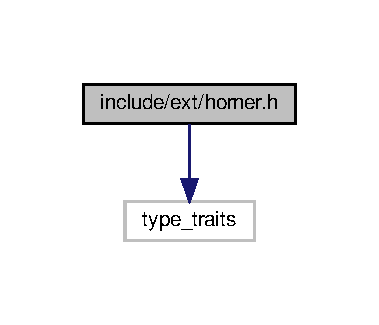
\includegraphics[width=182pt]{horner_8h__incl}
\end{center}
\end{figure}
\subsection*{Namespaces}
\begin{DoxyCompactItemize}
\item 
 \hyperlink{namespace____gnu__cxx}{\+\_\+\+\_\+gnu\+\_\+cxx}
\end{DoxyCompactItemize}
\subsection*{Functions}
\begin{DoxyCompactItemize}
\item 
{\footnotesize template$<$typename \+\_\+\+ArgT , typename \+\_\+\+Coef0 $>$ }\\constexpr std\+::conditional\+\_\+t$<$ std\+::is\+\_\+integral$<$ \+\_\+\+ArgT $>$\+::value, double, \+\_\+\+ArgT $>$ \hyperlink{namespace____gnu__cxx_a2e77239e9d41f55a99755f285ba3d518}{\+\_\+\+\_\+gnu\+\_\+cxx\+::horner} (\+\_\+\+ArgT \+\_\+\+\_\+x, \+\_\+\+Coef0 \+\_\+\+\_\+c0)
\item 
{\footnotesize template$<$typename \+\_\+\+ArgT , typename \+\_\+\+Coef0 , typename... \+\_\+\+Coef$>$ }\\constexpr std\+::conditional\+\_\+t$<$ std\+::is\+\_\+integral$<$ \+\_\+\+ArgT $>$\+::value, double, \+\_\+\+ArgT $>$ \hyperlink{namespace____gnu__cxx_a027e4b11b3b25078522220207c2d7f36}{\+\_\+\+\_\+gnu\+\_\+cxx\+::horner} (\+\_\+\+ArgT \+\_\+\+\_\+x, \+\_\+\+Coef0 \+\_\+\+\_\+c0, \+\_\+\+Coef... \+\_\+\+\_\+c)
\item 
{\footnotesize template$<$typename \+\_\+\+ArgT , typename \+\_\+\+Coef0 $>$ }\\constexpr std\+::conditional\+\_\+t$<$ std\+::is\+\_\+integral$<$ \+\_\+\+ArgT $>$\+::value, double, \+\_\+\+ArgT $>$ \hyperlink{namespace____gnu__cxx_af87123557fba351af5069ed8d1b99ec1}{\+\_\+\+\_\+gnu\+\_\+cxx\+::horner\+\_\+big\+\_\+end} (\+\_\+\+ArgT, \+\_\+\+Coef0 \+\_\+\+\_\+c0)
\item 
{\footnotesize template$<$typename \+\_\+\+ArgT , typename \+\_\+\+Coef1 , typename \+\_\+\+Coef0 $>$ }\\constexpr std\+::conditional\+\_\+t$<$ std\+::is\+\_\+integral$<$ \+\_\+\+ArgT $>$\+::value, double, \+\_\+\+ArgT $>$ \hyperlink{namespace____gnu__cxx_a546a72f007105e3ba32df87d7463edf7}{\+\_\+\+\_\+gnu\+\_\+cxx\+::horner\+\_\+big\+\_\+end} (\+\_\+\+ArgT \+\_\+\+\_\+x, \+\_\+\+Coef1 \+\_\+\+\_\+c1, \+\_\+\+Coef0 \+\_\+\+\_\+c0)
\item 
{\footnotesize template$<$typename \+\_\+\+ArgT , typename \+\_\+\+CoefN , typename \+\_\+\+Coef\+Nm1 , typename... \+\_\+\+Coef$>$ }\\constexpr std\+::conditional\+\_\+t$<$ std\+::is\+\_\+integral$<$ \+\_\+\+ArgT $>$\+::value, double, \+\_\+\+ArgT $>$ \hyperlink{namespace____gnu__cxx_afda9e3a1e351db85a89d4e6434576159}{\+\_\+\+\_\+gnu\+\_\+cxx\+::horner\+\_\+big\+\_\+end} (\+\_\+\+ArgT \+\_\+\+\_\+x, \+\_\+\+CoefN \+\_\+\+\_\+cn, \+\_\+\+Coef\+Nm1 \+\_\+\+\_\+cnm1, \+\_\+\+Coef... \+\_\+\+\_\+c)
\end{DoxyCompactItemize}


\subsection{Detailed Description}
Class declaration for Horner polynomial evaluation.

This file is a G\+NU extension to the Standard C++ Library. 
\hypertarget{polynomial_8h}{}\section{include/ext/polynomial.h File Reference}
\label{polynomial_8h}\index{include/ext/polynomial.\+h@{include/ext/polynomial.\+h}}
{\ttfamily \#include $<$initializer\+\_\+list$>$}\newline
{\ttfamily \#include $<$vector$>$}\newline
{\ttfamily \#include $<$iosfwd$>$}\newline
{\ttfamily \#include $<$limits$>$}\newline
{\ttfamily \#include $<$array$>$}\newline
{\ttfamily \#include $<$utility$>$}\newline
{\ttfamily \#include \char`\"{}polynomial.\+tcc\char`\"{}}\newline
Include dependency graph for polynomial.\+h\+:
\nopagebreak
\begin{figure}[H]
\begin{center}
\leavevmode
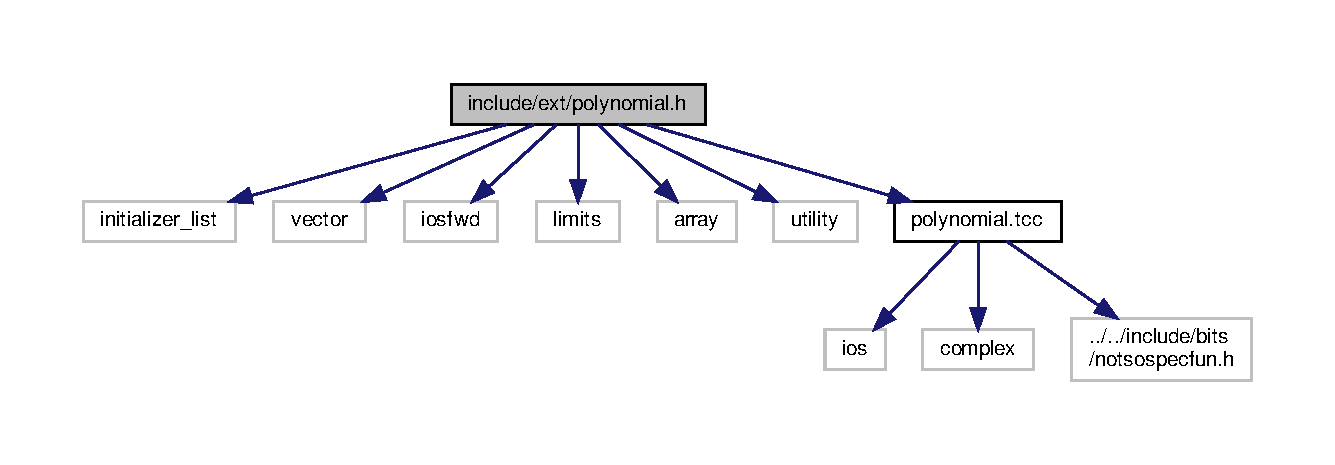
\includegraphics[width=350pt]{polynomial_8h__incl}
\end{center}
\end{figure}
This graph shows which files directly or indirectly include this file\+:
\nopagebreak
\begin{figure}[H]
\begin{center}
\leavevmode
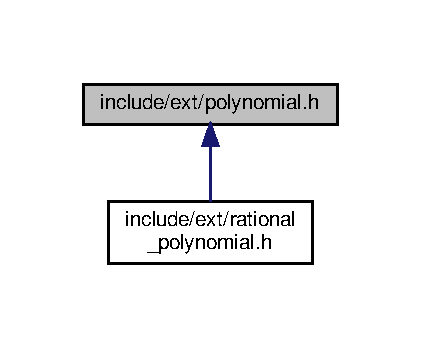
\includegraphics[width=202pt]{polynomial_8h__dep__incl}
\end{center}
\end{figure}
\subsection*{Classes}
\begin{DoxyCompactItemize}
\item 
struct \hyperlink{struct____gnu__cxx_1_1____has__imag__t}{\+\_\+\+\_\+gnu\+\_\+cxx\+::\+\_\+\+\_\+has\+\_\+imag\+\_\+t$<$ typename, typename $>$}
\item 
struct \hyperlink{struct____gnu__cxx_1_1____has__imag__t_3_01T_00_01std_1_1void__t_3_01decltype_07std_1_1declval_389ee8aaba7dec2e199e7ad81d6cda763}{\+\_\+\+\_\+gnu\+\_\+cxx\+::\+\_\+\+\_\+has\+\_\+imag\+\_\+t$<$ T, std\+::void\+\_\+t$<$ decltype(std\+::declval$<$ T \& $>$().\+imag())$>$ $>$}
\item 
class \hyperlink{class____gnu__cxx_1_1__Polynomial}{\+\_\+\+\_\+gnu\+\_\+cxx\+::\+\_\+\+Polynomial$<$ \+\_\+\+Tp $>$}
\begin{DoxyCompactList}\small\item\em A dense polynomial class with a contiguous array of coefficients. The coefficients are lowest-\/order first\+: \[ P(x) = a_0 + a_1 x + ... + a_n x^n \]. \end{DoxyCompactList}\item 
class \hyperlink{classstd_1_1complex}{std\+::complex$<$ \+\_\+\+Tp $>$}
\end{DoxyCompactItemize}
\subsection*{Namespaces}
\begin{DoxyCompactItemize}
\item 
 \hyperlink{namespace____gnu__cxx}{\+\_\+\+\_\+gnu\+\_\+cxx}
\item 
 \hyperlink{namespacestd}{std}
\end{DoxyCompactItemize}
\subsection*{Functions}
\begin{DoxyCompactItemize}
\item 
{\footnotesize template$<$typename \+\_\+\+Tp $>$ }\\void \hyperlink{namespace____gnu__cxx_abe506cf34c921c378a681f0de31d49a5}{\+\_\+\+\_\+gnu\+\_\+cxx\+::divmod} (const \+\_\+\+Polynomial$<$ \+\_\+\+Tp $>$ \&\+\_\+\+\_\+pa, const \+\_\+\+Polynomial$<$ \+\_\+\+Tp $>$ \&\+\_\+\+\_\+pb, \+\_\+\+Polynomial$<$ \+\_\+\+Tp $>$ \&\+\_\+\+\_\+quo, \+\_\+\+Polynomial$<$ \+\_\+\+Tp $>$ \&\+\_\+\+\_\+rem)
\item 
{\footnotesize template$<$typename \+\_\+\+Tp $>$ }\\\hyperlink{namespace____gnu__cxx_a2af747c0e255f3fae4d9f118c2817e1a}{\+\_\+\+\_\+gnu\+\_\+cxx\+::get\+\_\+scale} (const \+\_\+\+Polynomial$<$ \+\_\+\+Tp $>$ \&\+\_\+\+\_\+poly)
\item 
{\footnotesize template$<$typename \+\_\+\+Tp $>$ }\\\hyperlink{namespace____gnu__cxx_a1a8bae104a6509f4e458d155acaf0476}{\+\_\+\+\_\+gnu\+\_\+cxx\+::get\+\_\+scale} (const \+\_\+\+Tp \&\+\_\+\+\_\+x)
\item 
{\footnotesize template$<$typename \+\_\+\+Tp $>$ }\\bool \hyperlink{namespace____gnu__cxx_a1279934a2d6df66704c6eab9113b0f97}{\+\_\+\+\_\+gnu\+\_\+cxx\+::operator!=} (const \+\_\+\+Polynomial$<$ \+\_\+\+Tp $>$ \&\+\_\+\+\_\+pa, const \+\_\+\+Polynomial$<$ \+\_\+\+Tp $>$ \&\+\_\+\+\_\+pb)
\item 
{\footnotesize template$<$typename \+\_\+\+Tp , typename \+\_\+\+Up $>$ }\\\+\_\+\+Polynomial$<$ decltype(\+\_\+\+Tp()/\+\_\+\+Up())$>$ \hyperlink{namespace____gnu__cxx_a3132828069a740986e97f1db8e07325c}{\+\_\+\+\_\+gnu\+\_\+cxx\+::operator\%} (const \+\_\+\+Polynomial$<$ \+\_\+\+Tp $>$ \&\+\_\+\+\_\+poly, const \+\_\+\+Up \&\+\_\+\+\_\+x)
\item 
{\footnotesize template$<$typename \+\_\+\+Tp , typename \+\_\+\+Up $>$ }\\\+\_\+\+Polynomial$<$ decltype(\+\_\+\+Tp()/\+\_\+\+Up())$>$ \hyperlink{namespace____gnu__cxx_a13dae497264694313717a5aa70407de5}{\+\_\+\+\_\+gnu\+\_\+cxx\+::operator\%} (const \+\_\+\+Polynomial$<$ \+\_\+\+Tp $>$ \&\+\_\+\+\_\+pa, const \+\_\+\+Polynomial$<$ \+\_\+\+Up $>$ \&\+\_\+\+\_\+pb)
\item 
{\footnotesize template$<$typename \+\_\+\+Tp , typename \+\_\+\+Up $>$ }\\\+\_\+\+Polynomial$<$ decltype(\+\_\+\+Tp()/\+\_\+\+Up())$>$ \hyperlink{namespace____gnu__cxx_a2d1e6cb96943b2c99f71cf77a7247e77}{\+\_\+\+\_\+gnu\+\_\+cxx\+::operator\%} (const \+\_\+\+Tp \&\+\_\+\+\_\+x, const \+\_\+\+Polynomial$<$ \+\_\+\+Up $>$ \&\+\_\+\+\_\+poly)
\item 
{\footnotesize template$<$typename \+\_\+\+Tp , typename \+\_\+\+Up $>$ }\\\+\_\+\+Polynomial$<$ decltype(\+\_\+\+Tp() $\ast$\+\_\+\+Up())$>$ \hyperlink{namespace____gnu__cxx_a1d0b1e9322fd407848b43cecab1ab9ae}{\+\_\+\+\_\+gnu\+\_\+cxx\+::operator$\ast$} (const \+\_\+\+Polynomial$<$ \+\_\+\+Tp $>$ \&\+\_\+\+\_\+poly, const \+\_\+\+Up \&\+\_\+\+\_\+x)
\item 
{\footnotesize template$<$typename \+\_\+\+Tp , typename \+\_\+\+Up $>$ }\\\+\_\+\+Polynomial$<$ decltype(\+\_\+\+Tp() $\ast$\+\_\+\+Up())$>$ \hyperlink{namespace____gnu__cxx_a2f76fd6f7c2c9e64fba1d5892844f26b}{\+\_\+\+\_\+gnu\+\_\+cxx\+::operator$\ast$} (const \+\_\+\+Polynomial$<$ \+\_\+\+Tp $>$ \&\+\_\+\+\_\+pa, const \+\_\+\+Polynomial$<$ \+\_\+\+Up $>$ \&\+\_\+\+\_\+pb)
\item 
{\footnotesize template$<$typename \+\_\+\+Tp , typename \+\_\+\+Up $>$ }\\\+\_\+\+Polynomial$<$ decltype(\+\_\+\+Tp() $\ast$\+\_\+\+Up())$>$ \hyperlink{namespace____gnu__cxx_ac79cfe2d37e5d8116fcf51911c21c253}{\+\_\+\+\_\+gnu\+\_\+cxx\+::operator$\ast$} (const \+\_\+\+Tp \&\+\_\+\+\_\+x, const \+\_\+\+Polynomial$<$ \+\_\+\+Up $>$ \&\+\_\+\+\_\+poly)
\item 
{\footnotesize template$<$typename \+\_\+\+Tp , typename \+\_\+\+Up $>$ }\\\+\_\+\+Polynomial$<$ decltype(\+\_\+\+Tp()+\+\_\+\+Up())$>$ \hyperlink{namespace____gnu__cxx_a2b408e7a7e5d2ec6879b8e40f7f5de3e}{\+\_\+\+\_\+gnu\+\_\+cxx\+::operator+} (const \+\_\+\+Polynomial$<$ \+\_\+\+Tp $>$ \&\+\_\+\+\_\+poly, const \+\_\+\+Up \&\+\_\+\+\_\+x)
\item 
{\footnotesize template$<$typename \+\_\+\+Tp , typename \+\_\+\+Up $>$ }\\\+\_\+\+Polynomial$<$ decltype(\+\_\+\+Tp()+\+\_\+\+Up())$>$ \hyperlink{namespace____gnu__cxx_ada8a28005b5f71563bec55c71e03029b}{\+\_\+\+\_\+gnu\+\_\+cxx\+::operator+} (const \+\_\+\+Polynomial$<$ \+\_\+\+Tp $>$ \&\+\_\+\+\_\+pa, const \+\_\+\+Polynomial$<$ \+\_\+\+Up $>$ \&\+\_\+\+\_\+pb)
\item 
{\footnotesize template$<$typename \+\_\+\+Tp , typename \+\_\+\+Up $>$ }\\\+\_\+\+Polynomial$<$ decltype(\+\_\+\+Tp()+\+\_\+\+Up())$>$ \hyperlink{namespace____gnu__cxx_ac9f58ced995b65628b5715c885569cb7}{\+\_\+\+\_\+gnu\+\_\+cxx\+::operator+} (const \+\_\+\+Tp \&\+\_\+\+\_\+x, const \+\_\+\+Polynomial$<$ \+\_\+\+Up $>$ \&\+\_\+\+\_\+poly)
\item 
{\footnotesize template$<$typename \+\_\+\+Tp , typename \+\_\+\+Up $>$ }\\\+\_\+\+Polynomial$<$ decltype(\+\_\+\+Tp() -\/ \+\_\+\+Up())$>$ \hyperlink{namespace____gnu__cxx_abc583ac0684f0aff079c6014f3d84c1d}{\+\_\+\+\_\+gnu\+\_\+cxx\+::operator-\/} (const \+\_\+\+Polynomial$<$ \+\_\+\+Tp $>$ \&\+\_\+\+\_\+poly, const \+\_\+\+Up \&\+\_\+\+\_\+x)
\item 
{\footnotesize template$<$typename \+\_\+\+Tp , typename \+\_\+\+Up $>$ }\\\+\_\+\+Polynomial$<$ decltype(\+\_\+\+Tp() -\/ \+\_\+\+Up())$>$ \hyperlink{namespace____gnu__cxx_a4609eee7a71e3be3a103df9556fab9b4}{\+\_\+\+\_\+gnu\+\_\+cxx\+::operator-\/} (const \+\_\+\+Polynomial$<$ \+\_\+\+Tp $>$ \&\+\_\+\+\_\+pa, const \+\_\+\+Polynomial$<$ \+\_\+\+Up $>$ \&\+\_\+\+\_\+pb)
\item 
{\footnotesize template$<$typename \+\_\+\+Tp , typename \+\_\+\+Up $>$ }\\\+\_\+\+Polynomial$<$ decltype(\+\_\+\+Tp() -\/ \+\_\+\+Up())$>$ \hyperlink{namespace____gnu__cxx_acc72fd3c1efcf09698d30d42c4a1eb1b}{\+\_\+\+\_\+gnu\+\_\+cxx\+::operator-\/} (const \+\_\+\+Tp \&\+\_\+\+\_\+x, const \+\_\+\+Polynomial$<$ \+\_\+\+Up $>$ \&\+\_\+\+\_\+poly)
\item 
{\footnotesize template$<$typename \+\_\+\+Tp , typename \+\_\+\+Up $>$ }\\\+\_\+\+Polynomial$<$ decltype(\+\_\+\+Tp()/\+\_\+\+Up())$>$ \hyperlink{namespace____gnu__cxx_a5fd356349013bd60a41010cbf502444b}{\+\_\+\+\_\+gnu\+\_\+cxx\+::operator/} (const \+\_\+\+Polynomial$<$ \+\_\+\+Tp $>$ \&\+\_\+\+\_\+poly, const \+\_\+\+Up \&\+\_\+\+\_\+x)
\item 
{\footnotesize template$<$typename \+\_\+\+Tp , typename \+\_\+\+Up $>$ }\\\+\_\+\+Polynomial$<$ decltype(\+\_\+\+Tp()/\+\_\+\+Up())$>$ \hyperlink{namespace____gnu__cxx_a6ba146c479b383e9ba26760c847e3dc6}{\+\_\+\+\_\+gnu\+\_\+cxx\+::operator/} (const \+\_\+\+Polynomial$<$ \+\_\+\+Tp $>$ \&\+\_\+\+\_\+pa, const \+\_\+\+Polynomial$<$ \+\_\+\+Up $>$ \&\+\_\+\+\_\+pb)
\item 
{\footnotesize template$<$typename \+\_\+\+Tp , typename \+\_\+\+Up $>$ }\\\+\_\+\+Polynomial$<$ decltype(\+\_\+\+Tp()/\+\_\+\+Up())$>$ \hyperlink{namespace____gnu__cxx_a4c1b4c46ffc6c41fb5b5d1a4293ca563}{\+\_\+\+\_\+gnu\+\_\+cxx\+::operator/} (const \+\_\+\+Tp \&\+\_\+\+\_\+x, const \+\_\+\+Polynomial$<$ \+\_\+\+Up $>$ \&\+\_\+\+\_\+poly)
\item 
{\footnotesize template$<$typename CharT , typename Traits , typename \+\_\+\+Tp $>$ }\\std\+::basic\+\_\+ostream$<$ CharT, Traits $>$ \& \hyperlink{namespace____gnu__cxx_ad713743dbfc30fba653621d1f7e99d3c}{\+\_\+\+\_\+gnu\+\_\+cxx\+::operator$<$$<$} (std\+::basic\+\_\+ostream$<$ CharT, Traits $>$ \&\+\_\+\+\_\+os, const \+\_\+\+Polynomial$<$ \+\_\+\+Tp $>$ \&\+\_\+\+\_\+poly)
\item 
{\footnotesize template$<$typename \+\_\+\+Tp $>$ }\\bool \hyperlink{namespace____gnu__cxx_a7427db234bb8c8aab722a3196e898215}{\+\_\+\+\_\+gnu\+\_\+cxx\+::operator==} (const \+\_\+\+Polynomial$<$ \+\_\+\+Tp $>$ \&\+\_\+\+\_\+pa, const \+\_\+\+Polynomial$<$ \+\_\+\+Tp $>$ \&\+\_\+\+\_\+pb)
\item 
{\footnotesize template$<$typename CharT , typename Traits , typename \+\_\+\+Tp $>$ }\\std\+::basic\+\_\+istream$<$ CharT, Traits $>$ \& \hyperlink{namespace____gnu__cxx_acf7d03318756578d08f672212cd91234}{\+\_\+\+\_\+gnu\+\_\+cxx\+::operator$>$$>$} (std\+::basic\+\_\+istream$<$ CharT, Traits $>$ \&\+\_\+\+\_\+is, \+\_\+\+Polynomial$<$ \+\_\+\+Tp $>$ \&\+\_\+\+\_\+poly)
\item 
{\footnotesize template$<$typename \+\_\+\+Tp $>$ }\\void \hyperlink{namespace____gnu__cxx_a10d002d78eb10d846416335ca9599c7a}{\+\_\+\+\_\+gnu\+\_\+cxx\+::swap} (\+\_\+\+Polynomial$<$ \+\_\+\+Tp $>$ \&\+\_\+\+\_\+pa, \+\_\+\+Polynomial$<$ \+\_\+\+Tp $>$ \&\+\_\+\+\_\+pb) noexcept(noexcept(\+\_\+\+\_\+pa.\+swap(\+\_\+\+\_\+pb)))
\end{DoxyCompactItemize}
\subsection*{Variables}
\begin{DoxyCompactItemize}
\item 
{\footnotesize template$<$typename T $>$ }\\constexpr auto \hyperlink{namespace____gnu__cxx_afa2404a914b06f950f3a46e75aca51a9}{\+\_\+\+\_\+gnu\+\_\+cxx\+::\+\_\+\+\_\+has\+\_\+imag\+\_\+v} = \+\_\+\+\_\+has\+\_\+imag\+\_\+t$<$T$>$\+::value
\end{DoxyCompactItemize}


\subsection{Detailed Description}
Class declaration for a dense monovariate polynomial.

This file is a G\+NU extension to the Standard C++ Library.

This file contains the declaration of a dense-\/polynomial class. 
\hypertarget{polynomial_8tcc}{}\section{include/ext/polynomial.tcc File Reference}
\label{polynomial_8tcc}\index{include/ext/polynomial.\+tcc@{include/ext/polynomial.\+tcc}}
{\ttfamily \#include $<$ios$>$}\newline
{\ttfamily \#include $<$complex$>$}\newline
{\ttfamily \#include \char`\"{}../../include/bits/notsospecfun.\+h\char`\"{}}\newline
Include dependency graph for polynomial.\+tcc\+:
\nopagebreak
\begin{figure}[H]
\begin{center}
\leavevmode
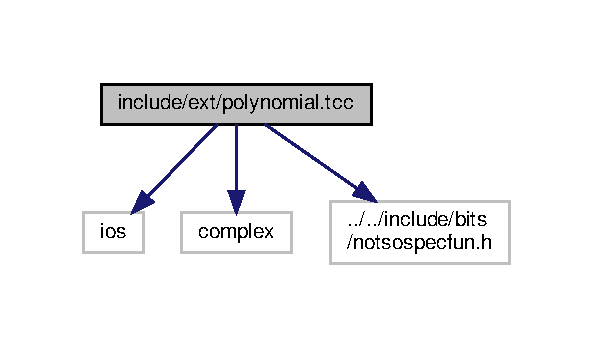
\includegraphics[width=285pt]{polynomial_8tcc__incl}
\end{center}
\end{figure}
This graph shows which files directly or indirectly include this file\+:
\nopagebreak
\begin{figure}[H]
\begin{center}
\leavevmode
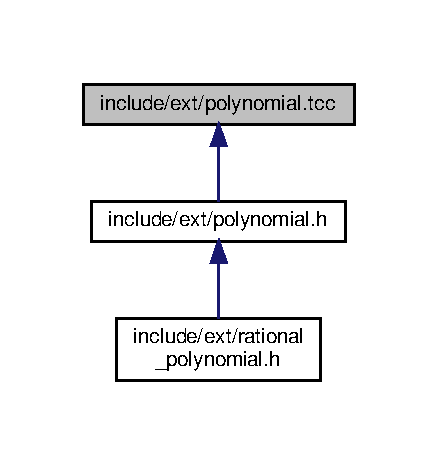
\includegraphics[width=210pt]{polynomial_8tcc__dep__incl}
\end{center}
\end{figure}
\subsection*{Namespaces}
\begin{DoxyCompactItemize}
\item 
 \hyperlink{namespace____gnu__cxx}{\+\_\+\+\_\+gnu\+\_\+cxx}
\end{DoxyCompactItemize}
\subsection*{Macros}
\begin{DoxyCompactItemize}
\item 
\#define \hyperlink{polynomial_8tcc_af5a65c717a211a48a4cf31df10b4537a}{\+\_\+\+E\+X\+T\+\_\+\+P\+O\+L\+Y\+N\+O\+M\+I\+A\+L\+\_\+\+T\+CC}~1
\begin{DoxyCompactList}\small\item\em A guard for the polynomial class implementation header. \end{DoxyCompactList}\end{DoxyCompactItemize}
\subsection*{Functions}
\begin{DoxyCompactItemize}
\item 
{\footnotesize template$<$typename \+\_\+\+Tp $>$ }\\void \hyperlink{namespace____gnu__cxx_abe506cf34c921c378a681f0de31d49a5}{\+\_\+\+\_\+gnu\+\_\+cxx\+::divmod} (const \+\_\+\+Polynomial$<$ \+\_\+\+Tp $>$ \&\+\_\+\+\_\+pa, const \+\_\+\+Polynomial$<$ \+\_\+\+Tp $>$ \&\+\_\+\+\_\+pb, \+\_\+\+Polynomial$<$ \+\_\+\+Tp $>$ \&\+\_\+\+\_\+quo, \+\_\+\+Polynomial$<$ \+\_\+\+Tp $>$ \&\+\_\+\+\_\+rem)
\item 
{\footnotesize template$<$typename CharT , typename Traits , typename \+\_\+\+Tp $>$ }\\std\+::basic\+\_\+ostream$<$ CharT, Traits $>$ \& \hyperlink{namespace____gnu__cxx_ad713743dbfc30fba653621d1f7e99d3c}{\+\_\+\+\_\+gnu\+\_\+cxx\+::operator$<$$<$} (std\+::basic\+\_\+ostream$<$ CharT, Traits $>$ \&\+\_\+\+\_\+os, const \+\_\+\+Polynomial$<$ \+\_\+\+Tp $>$ \&\+\_\+\+\_\+poly)
\item 
{\footnotesize template$<$typename CharT , typename Traits , typename \+\_\+\+Tp $>$ }\\std\+::basic\+\_\+istream$<$ CharT, Traits $>$ \& \hyperlink{namespace____gnu__cxx_acf7d03318756578d08f672212cd91234}{\+\_\+\+\_\+gnu\+\_\+cxx\+::operator$>$$>$} (std\+::basic\+\_\+istream$<$ CharT, Traits $>$ \&\+\_\+\+\_\+is, \+\_\+\+Polynomial$<$ \+\_\+\+Tp $>$ \&\+\_\+\+\_\+poly)
\end{DoxyCompactItemize}
\subsection*{Variables}
\begin{DoxyCompactItemize}
\item 
$\ast$ \hyperlink{namespace____gnu__cxx_ab693ea357b6429b331e0bf09f9442385}{\+\_\+\+\_\+gnu\+\_\+cxx\+::\+\_\+\+Up}
\end{DoxyCompactItemize}


\subsection{Detailed Description}
Out-\/of-\/line definitions of members for a dense monovariate polynomial.

This file is a G\+NU extension to the Standard C++ Library. This file contains the out-\/of-\/line implementations of the polynomial class.

\begin{DoxySeeAlso}{See also}
\hyperlink{polynomial_8h}{polynomial.\+h} 
\end{DoxySeeAlso}


\subsection{Macro Definition Documentation}
\mbox{\Hypertarget{polynomial_8tcc_af5a65c717a211a48a4cf31df10b4537a}\label{polynomial_8tcc_af5a65c717a211a48a4cf31df10b4537a}} 
\index{polynomial.\+tcc@{polynomial.\+tcc}!\+\_\+\+E\+X\+T\+\_\+\+P\+O\+L\+Y\+N\+O\+M\+I\+A\+L\+\_\+\+T\+CC@{\+\_\+\+E\+X\+T\+\_\+\+P\+O\+L\+Y\+N\+O\+M\+I\+A\+L\+\_\+\+T\+CC}}
\index{\+\_\+\+E\+X\+T\+\_\+\+P\+O\+L\+Y\+N\+O\+M\+I\+A\+L\+\_\+\+T\+CC@{\+\_\+\+E\+X\+T\+\_\+\+P\+O\+L\+Y\+N\+O\+M\+I\+A\+L\+\_\+\+T\+CC}!polynomial.\+tcc@{polynomial.\+tcc}}
\subsubsection{\texorpdfstring{\+\_\+\+E\+X\+T\+\_\+\+P\+O\+L\+Y\+N\+O\+M\+I\+A\+L\+\_\+\+T\+CC}{\_EXT\_POLYNOMIAL\_TCC}}
{\footnotesize\ttfamily \#define \+\_\+\+E\+X\+T\+\_\+\+P\+O\+L\+Y\+N\+O\+M\+I\+A\+L\+\_\+\+T\+CC~1}



A guard for the polynomial class implementation header. 



Definition at line 41 of file polynomial.\+tcc.


\hypertarget{rational__polynomial_8h}{}\section{include/ext/rational\+\_\+polynomial.h File Reference}
\label{rational__polynomial_8h}\index{include/ext/rational\+\_\+polynomial.\+h@{include/ext/rational\+\_\+polynomial.\+h}}
{\ttfamily \#include $<$iostream$>$}\newline
{\ttfamily \#include \char`\"{}polynomial.\+h\char`\"{}}\newline
Include dependency graph for rational\+\_\+polynomial.\+h\+:
\nopagebreak
\begin{figure}[H]
\begin{center}
\leavevmode
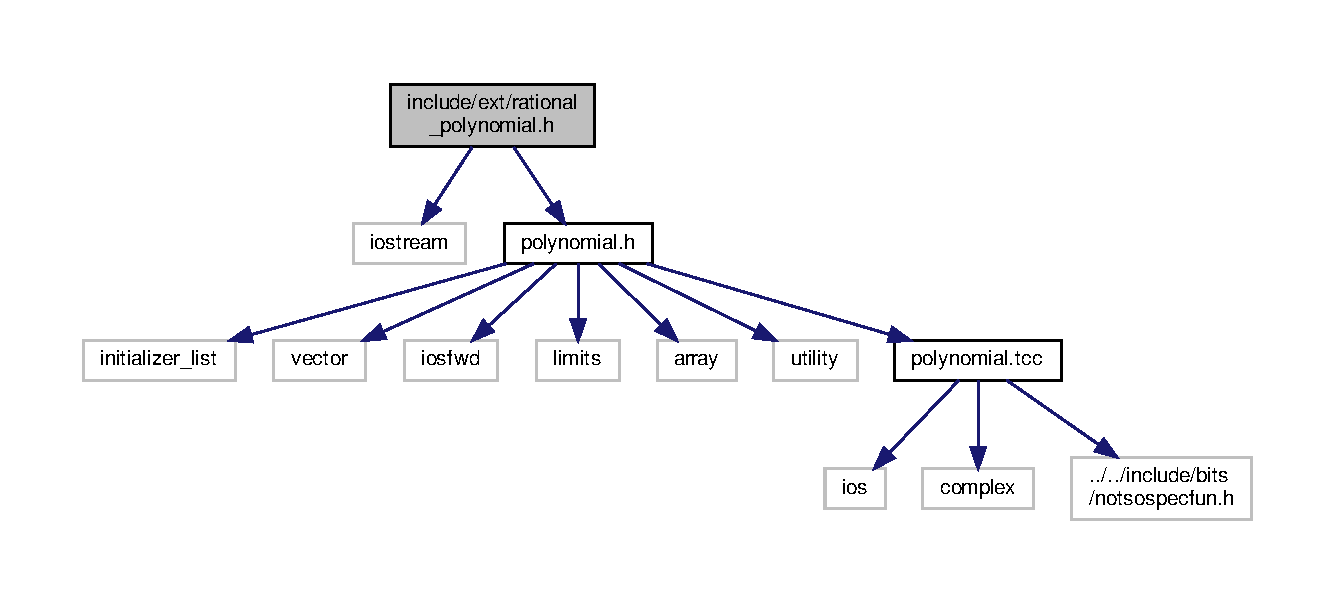
\includegraphics[width=350pt]{rational__polynomial_8h__incl}
\end{center}
\end{figure}
\subsection*{Classes}
\begin{DoxyCompactItemize}
\item 
class \hyperlink{class____gnu__cxx_1_1__RationalPolynomial}{\+\_\+\+\_\+gnu\+\_\+cxx\+::\+\_\+\+Rational\+Polynomial$<$ \+\_\+\+Tp $>$}
\end{DoxyCompactItemize}
\subsection*{Namespaces}
\begin{DoxyCompactItemize}
\item 
 \hyperlink{namespace____gnu__cxx}{\+\_\+\+\_\+gnu\+\_\+cxx}
\end{DoxyCompactItemize}
\subsection*{Functions}
\begin{DoxyCompactItemize}
\item 
{\footnotesize template$<$typename CharT , typename Traits , typename \+\_\+\+Tp $>$ }\\std\+::basic\+\_\+ostream$<$ CharT, Traits $>$ \& \hyperlink{namespace____gnu__cxx_a424044092ac184bfa1d17beb1b12e071}{\+\_\+\+\_\+gnu\+\_\+cxx\+::operator$<$$<$} (std\+::basic\+\_\+ostream$<$ CharT, Traits $>$ \&\+\_\+\+\_\+os, const \+\_\+\+Rational\+Polynomial$<$ \+\_\+\+Tp $>$ \&\+\_\+\+\_\+poly)
\item 
{\footnotesize template$<$typename CharT , typename Traits , typename \+\_\+\+Tp $>$ }\\std\+::basic\+\_\+istream$<$ CharT, Traits $>$ \& \hyperlink{namespace____gnu__cxx_a71511bc907f332ce9bb925c953f11714}{\+\_\+\+\_\+gnu\+\_\+cxx\+::operator$>$$>$} (std\+::basic\+\_\+istream$<$ CharT, Traits $>$ \&\+\_\+\+\_\+is, \+\_\+\+Rational\+Polynomial$<$ \+\_\+\+Tp $>$ \&\+\_\+\+\_\+poly)
\end{DoxyCompactItemize}


\subsection{Detailed Description}
This file is a G\+NU extension to the Standard C++ Library.

This file contains the declaration of a ratio of two polynomials. \begin{DoxySeeAlso}{See also}
\hyperlink{polynomial_8h}{polynomial.\+h} 
\end{DoxySeeAlso}

\hypertarget{solution_8h}{}\section{include/ext/solution.h File Reference}
\label{solution_8h}\index{include/ext/solution.\+h@{include/ext/solution.\+h}}
{\ttfamily \#include $<$complex$>$}\newline
{\ttfamily \#include $<$variant$>$}\newline
{\ttfamily \#include $<$iosfwd$>$}\newline
Include dependency graph for solution.\+h\+:
\nopagebreak
\begin{figure}[H]
\begin{center}
\leavevmode
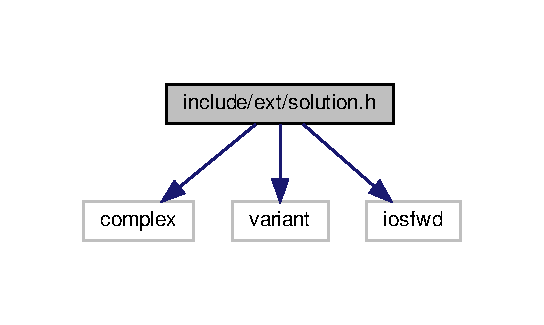
\includegraphics[width=261pt]{solution_8h__incl}
\end{center}
\end{figure}
This graph shows which files directly or indirectly include this file\+:
\nopagebreak
\begin{figure}[H]
\begin{center}
\leavevmode
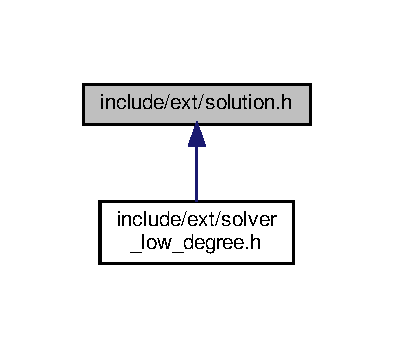
\includegraphics[width=189pt]{solution_8h__dep__incl}
\end{center}
\end{figure}
\subsection*{Namespaces}
\begin{DoxyCompactItemize}
\item 
 \hyperlink{namespace____gnu__cxx}{\+\_\+\+\_\+gnu\+\_\+cxx}
\item 
 \hyperlink{namespacestd}{std}
\end{DoxyCompactItemize}
\subsection*{Typedefs}
\begin{DoxyCompactItemize}
\item 
{\footnotesize template$<$typename \+\_\+\+Real $>$ }\\using \hyperlink{namespace____gnu__cxx_ae20ea642de50eb361074c62676b0159c}{\+\_\+\+\_\+gnu\+\_\+cxx\+::solution\+\_\+t} = std\+::variant$<$ std\+::monostate, \+\_\+\+Real, \hyperlink{classstd_1_1complex}{std\+::complex}$<$ \+\_\+\+Real $>$ $>$
\end{DoxyCompactItemize}
\subsection*{Functions}
\begin{DoxyCompactItemize}
\item 
{\footnotesize template$<$typename \+\_\+\+Real $>$ }\\constexpr \+\_\+\+Real \hyperlink{namespace____gnu__cxx_ab9eb9db3560f504f8cd25a71bcb6ead5}{\+\_\+\+\_\+gnu\+\_\+cxx\+::abs} (const solution\+\_\+t$<$ \+\_\+\+Real $>$ \&\+\_\+\+\_\+x)
\item 
{\footnotesize template$<$typename \+\_\+\+Real $>$ }\\constexpr \+\_\+\+Real \hyperlink{namespace____gnu__cxx_a685dd0477f8454431bcfb404fa201c57}{\+\_\+\+\_\+gnu\+\_\+cxx\+::imag} (const solution\+\_\+t$<$ \+\_\+\+Real $>$ \&\+\_\+\+\_\+x)
\item 
{\footnotesize template$<$typename \+\_\+\+Real $>$ }\\constexpr bool \hyperlink{namespace____gnu__cxx_ac6649e26a3db551b4f945ccfcd3ce0a7}{\+\_\+\+\_\+gnu\+\_\+cxx\+::is\+\_\+valid} (const solution\+\_\+t$<$ \+\_\+\+Real $>$ \&\+\_\+\+\_\+x)
\item 
{\footnotesize template$<$typename \+\_\+\+Real $>$ }\\constexpr bool \hyperlink{namespacestd_a0f89c0cd89caea7c7413c22c4c7e21f9}{std\+::operator!=} (const \hyperlink{namespace____gnu__cxx_ae20ea642de50eb361074c62676b0159c}{\+\_\+\+\_\+gnu\+\_\+cxx\+::solution\+\_\+t}$<$ \+\_\+\+Real $>$ \&\+\_\+\+\_\+x, const \hyperlink{namespace____gnu__cxx_ae20ea642de50eb361074c62676b0159c}{\+\_\+\+\_\+gnu\+\_\+cxx\+::solution\+\_\+t}$<$ \+\_\+\+Real $>$ \&\+\_\+\+\_\+y)
\item 
{\footnotesize template$<$typename \+\_\+\+Real $>$ }\\bool \hyperlink{namespacestd_a88548a06c4013d8e23c70a25a48a8929}{std\+::operator!=} (const \hyperlink{namespace____gnu__cxx_ae20ea642de50eb361074c62676b0159c}{\+\_\+\+\_\+gnu\+\_\+cxx\+::solution\+\_\+t}$<$ \+\_\+\+Real $>$ \&\+\_\+\+\_\+x, \+\_\+\+Real \+\_\+\+\_\+y)
\item 
{\footnotesize template$<$typename \+\_\+\+Real $>$ }\\constexpr bool \hyperlink{namespacestd_ac8ab440760f8eab57232be8417861387}{std\+::operator!=} (\+\_\+\+Real \+\_\+\+\_\+x, const \hyperlink{namespace____gnu__cxx_ae20ea642de50eb361074c62676b0159c}{\+\_\+\+\_\+gnu\+\_\+cxx\+::solution\+\_\+t}$<$ \+\_\+\+Real $>$ \&\+\_\+\+\_\+y)
\item 
{\footnotesize template$<$typename \+\_\+\+Real $>$ }\\constexpr bool \hyperlink{namespacestd_a613014e2e7afb3c131c9530988e20417}{std\+::operator!=} (const \hyperlink{namespace____gnu__cxx_ae20ea642de50eb361074c62676b0159c}{\+\_\+\+\_\+gnu\+\_\+cxx\+::solution\+\_\+t}$<$ \+\_\+\+Real $>$ \&\+\_\+\+\_\+x, const \hyperlink{classstd_1_1complex}{std\+::complex}$<$ \+\_\+\+Real $>$ \&\+\_\+\+\_\+y)
\item 
{\footnotesize template$<$typename \+\_\+\+Real $>$ }\\constexpr bool \hyperlink{namespacestd_ad62f982d25741aa725c67cb3380782d9}{std\+::operator!=} (const \hyperlink{classstd_1_1complex}{std\+::complex}$<$ \+\_\+\+Real $>$ \&\+\_\+\+\_\+x, const \hyperlink{namespace____gnu__cxx_ae20ea642de50eb361074c62676b0159c}{\+\_\+\+\_\+gnu\+\_\+cxx\+::solution\+\_\+t}$<$ \+\_\+\+Real $>$ \&\+\_\+\+\_\+y)
\item 
{\footnotesize template$<$typename \+\_\+\+Real $>$ }\\constexpr \hyperlink{namespace____gnu__cxx_ae20ea642de50eb361074c62676b0159c}{\+\_\+\+\_\+gnu\+\_\+cxx\+::solution\+\_\+t}$<$ \+\_\+\+Real $>$ \hyperlink{namespacestd_afe761665ed44abc2edacac26cb45c645}{std\+::operator$\ast$} (const \hyperlink{namespace____gnu__cxx_ae20ea642de50eb361074c62676b0159c}{\+\_\+\+\_\+gnu\+\_\+cxx\+::solution\+\_\+t}$<$ \+\_\+\+Real $>$ \&\+\_\+\+\_\+x, const \hyperlink{namespace____gnu__cxx_ae20ea642de50eb361074c62676b0159c}{\+\_\+\+\_\+gnu\+\_\+cxx\+::solution\+\_\+t}$<$ \+\_\+\+Real $>$ \&\+\_\+\+\_\+y)
\item 
{\footnotesize template$<$typename \+\_\+\+Real $>$ }\\constexpr \hyperlink{namespace____gnu__cxx_ae20ea642de50eb361074c62676b0159c}{\+\_\+\+\_\+gnu\+\_\+cxx\+::solution\+\_\+t}$<$ \+\_\+\+Real $>$ \hyperlink{namespacestd_a13970e4b2bf6680ae3284c0f1117ea4d}{std\+::operator$\ast$} (const \hyperlink{namespace____gnu__cxx_ae20ea642de50eb361074c62676b0159c}{\+\_\+\+\_\+gnu\+\_\+cxx\+::solution\+\_\+t}$<$ \+\_\+\+Real $>$ \&\+\_\+\+\_\+x, \+\_\+\+Real \+\_\+\+\_\+y)
\item 
{\footnotesize template$<$typename \+\_\+\+Real $>$ }\\constexpr \hyperlink{namespace____gnu__cxx_ae20ea642de50eb361074c62676b0159c}{\+\_\+\+\_\+gnu\+\_\+cxx\+::solution\+\_\+t}$<$ \+\_\+\+Real $>$ \hyperlink{namespacestd_ab5d6a3adb4cf1cddc401e0465b832318}{std\+::operator$\ast$} (\+\_\+\+Real \+\_\+\+\_\+x, const \hyperlink{namespace____gnu__cxx_ae20ea642de50eb361074c62676b0159c}{\+\_\+\+\_\+gnu\+\_\+cxx\+::solution\+\_\+t}$<$ \+\_\+\+Real $>$ \&\+\_\+\+\_\+y)
\item 
{\footnotesize template$<$typename \+\_\+\+Real $>$ }\\constexpr \hyperlink{namespace____gnu__cxx_ae20ea642de50eb361074c62676b0159c}{\+\_\+\+\_\+gnu\+\_\+cxx\+::solution\+\_\+t}$<$ \+\_\+\+Real $>$ \hyperlink{namespacestd_acfa023cb6fb21c4285b73e1728cf340d}{std\+::operator$\ast$} (const \hyperlink{namespace____gnu__cxx_ae20ea642de50eb361074c62676b0159c}{\+\_\+\+\_\+gnu\+\_\+cxx\+::solution\+\_\+t}$<$ \+\_\+\+Real $>$ \&\+\_\+\+\_\+x, \hyperlink{classstd_1_1complex}{std\+::complex}$<$ \+\_\+\+Real $>$ \&\+\_\+\+\_\+y)
\item 
{\footnotesize template$<$typename \+\_\+\+Real $>$ }\\constexpr \hyperlink{namespace____gnu__cxx_ae20ea642de50eb361074c62676b0159c}{\+\_\+\+\_\+gnu\+\_\+cxx\+::solution\+\_\+t}$<$ \+\_\+\+Real $>$ \hyperlink{namespacestd_ae82d1f9ca11a46b93a33f2f89ce71305}{std\+::operator$\ast$} (\hyperlink{classstd_1_1complex}{std\+::complex}$<$ \+\_\+\+Real $>$ \&\+\_\+\+\_\+x, const \hyperlink{namespace____gnu__cxx_ae20ea642de50eb361074c62676b0159c}{\+\_\+\+\_\+gnu\+\_\+cxx\+::solution\+\_\+t}$<$ \+\_\+\+Real $>$ \&\+\_\+\+\_\+y)
\item 
{\footnotesize template$<$typename \+\_\+\+Real $>$ }\\constexpr \hyperlink{namespace____gnu__cxx_ae20ea642de50eb361074c62676b0159c}{\+\_\+\+\_\+gnu\+\_\+cxx\+::solution\+\_\+t}$<$ \+\_\+\+Real $>$ \hyperlink{namespacestd_a49a4eaaa2e023275443b1854bc90c77d}{std\+::operator+} (const \hyperlink{namespace____gnu__cxx_ae20ea642de50eb361074c62676b0159c}{\+\_\+\+\_\+gnu\+\_\+cxx\+::solution\+\_\+t}$<$ \+\_\+\+Real $>$ \&\+\_\+\+\_\+x)
\item 
{\footnotesize template$<$typename \+\_\+\+Real $>$ }\\constexpr \hyperlink{namespace____gnu__cxx_ae20ea642de50eb361074c62676b0159c}{\+\_\+\+\_\+gnu\+\_\+cxx\+::solution\+\_\+t}$<$ \+\_\+\+Real $>$ \hyperlink{namespacestd_ad34e888e243a1ad8303966f3cfe7a690}{std\+::operator+} (const \hyperlink{namespace____gnu__cxx_ae20ea642de50eb361074c62676b0159c}{\+\_\+\+\_\+gnu\+\_\+cxx\+::solution\+\_\+t}$<$ \+\_\+\+Real $>$ \&\+\_\+\+\_\+x, const \hyperlink{namespace____gnu__cxx_ae20ea642de50eb361074c62676b0159c}{\+\_\+\+\_\+gnu\+\_\+cxx\+::solution\+\_\+t}$<$ \+\_\+\+Real $>$ \&\+\_\+\+\_\+y)
\item 
{\footnotesize template$<$typename \+\_\+\+Real $>$ }\\constexpr \hyperlink{namespace____gnu__cxx_ae20ea642de50eb361074c62676b0159c}{\+\_\+\+\_\+gnu\+\_\+cxx\+::solution\+\_\+t}$<$ \+\_\+\+Real $>$ \hyperlink{namespacestd_a57af80492f51cac0e5c9cde7ea2ca845}{std\+::operator+} (const \hyperlink{namespace____gnu__cxx_ae20ea642de50eb361074c62676b0159c}{\+\_\+\+\_\+gnu\+\_\+cxx\+::solution\+\_\+t}$<$ \+\_\+\+Real $>$ \&\+\_\+\+\_\+x, \+\_\+\+Real \+\_\+\+\_\+y)
\item 
{\footnotesize template$<$typename \+\_\+\+Real $>$ }\\constexpr \hyperlink{namespace____gnu__cxx_ae20ea642de50eb361074c62676b0159c}{\+\_\+\+\_\+gnu\+\_\+cxx\+::solution\+\_\+t}$<$ \+\_\+\+Real $>$ \hyperlink{namespacestd_a6f47cf71b7277a461d5627a46748abe1}{std\+::operator+} (\+\_\+\+Real \+\_\+\+\_\+x, const \hyperlink{namespace____gnu__cxx_ae20ea642de50eb361074c62676b0159c}{\+\_\+\+\_\+gnu\+\_\+cxx\+::solution\+\_\+t}$<$ \+\_\+\+Real $>$ \&\+\_\+\+\_\+y)
\item 
{\footnotesize template$<$typename \+\_\+\+Real $>$ }\\constexpr \hyperlink{namespace____gnu__cxx_ae20ea642de50eb361074c62676b0159c}{\+\_\+\+\_\+gnu\+\_\+cxx\+::solution\+\_\+t}$<$ \+\_\+\+Real $>$ \hyperlink{namespacestd_a7c7a048cefad54d71198cecef43ff7bd}{std\+::operator+} (const \hyperlink{namespace____gnu__cxx_ae20ea642de50eb361074c62676b0159c}{\+\_\+\+\_\+gnu\+\_\+cxx\+::solution\+\_\+t}$<$ \+\_\+\+Real $>$ \&\+\_\+\+\_\+x, \hyperlink{classstd_1_1complex}{std\+::complex}$<$ \+\_\+\+Real $>$ \&\+\_\+\+\_\+y)
\item 
{\footnotesize template$<$typename \+\_\+\+Real $>$ }\\constexpr \hyperlink{namespace____gnu__cxx_ae20ea642de50eb361074c62676b0159c}{\+\_\+\+\_\+gnu\+\_\+cxx\+::solution\+\_\+t}$<$ \+\_\+\+Real $>$ \hyperlink{namespacestd_aa471e6e6583f0beced389171490d8684}{std\+::operator+} (\hyperlink{classstd_1_1complex}{std\+::complex}$<$ \+\_\+\+Real $>$ \&\+\_\+\+\_\+x, const \hyperlink{namespace____gnu__cxx_ae20ea642de50eb361074c62676b0159c}{\+\_\+\+\_\+gnu\+\_\+cxx\+::solution\+\_\+t}$<$ \+\_\+\+Real $>$ \&\+\_\+\+\_\+y)
\item 
{\footnotesize template$<$typename \+\_\+\+Real $>$ }\\constexpr \hyperlink{namespace____gnu__cxx_ae20ea642de50eb361074c62676b0159c}{\+\_\+\+\_\+gnu\+\_\+cxx\+::solution\+\_\+t}$<$ \+\_\+\+Real $>$ \hyperlink{namespacestd_a6cd0256e6734f6ff66ad5e4f9d4f1741}{std\+::operator-\/} (const \hyperlink{namespace____gnu__cxx_ae20ea642de50eb361074c62676b0159c}{\+\_\+\+\_\+gnu\+\_\+cxx\+::solution\+\_\+t}$<$ \+\_\+\+Real $>$ \&\+\_\+\+\_\+x)
\item 
{\footnotesize template$<$typename \+\_\+\+Real $>$ }\\constexpr \hyperlink{namespace____gnu__cxx_ae20ea642de50eb361074c62676b0159c}{\+\_\+\+\_\+gnu\+\_\+cxx\+::solution\+\_\+t}$<$ \+\_\+\+Real $>$ \hyperlink{namespacestd_ad3462eddf6b43f6e2d87b7a5fa2a2307}{std\+::operator-\/} (const \hyperlink{namespace____gnu__cxx_ae20ea642de50eb361074c62676b0159c}{\+\_\+\+\_\+gnu\+\_\+cxx\+::solution\+\_\+t}$<$ \+\_\+\+Real $>$ \&\+\_\+\+\_\+x, const \hyperlink{namespace____gnu__cxx_ae20ea642de50eb361074c62676b0159c}{\+\_\+\+\_\+gnu\+\_\+cxx\+::solution\+\_\+t}$<$ \+\_\+\+Real $>$ \&\+\_\+\+\_\+y)
\item 
{\footnotesize template$<$typename \+\_\+\+Real $>$ }\\constexpr \hyperlink{namespace____gnu__cxx_ae20ea642de50eb361074c62676b0159c}{\+\_\+\+\_\+gnu\+\_\+cxx\+::solution\+\_\+t}$<$ \+\_\+\+Real $>$ \hyperlink{namespacestd_a35af0b87e94fb38640fa36b7ec161645}{std\+::operator-\/} (const \hyperlink{namespace____gnu__cxx_ae20ea642de50eb361074c62676b0159c}{\+\_\+\+\_\+gnu\+\_\+cxx\+::solution\+\_\+t}$<$ \+\_\+\+Real $>$ \&\+\_\+\+\_\+x, \+\_\+\+Real \+\_\+\+\_\+y)
\item 
{\footnotesize template$<$typename \+\_\+\+Real $>$ }\\constexpr \hyperlink{namespace____gnu__cxx_ae20ea642de50eb361074c62676b0159c}{\+\_\+\+\_\+gnu\+\_\+cxx\+::solution\+\_\+t}$<$ \+\_\+\+Real $>$ \hyperlink{namespacestd_ae02c419877b95950c8c9630c6a4971a1}{std\+::operator-\/} (\+\_\+\+Real \+\_\+\+\_\+x, const \hyperlink{namespace____gnu__cxx_ae20ea642de50eb361074c62676b0159c}{\+\_\+\+\_\+gnu\+\_\+cxx\+::solution\+\_\+t}$<$ \+\_\+\+Real $>$ \&\+\_\+\+\_\+y)
\item 
{\footnotesize template$<$typename \+\_\+\+Real $>$ }\\constexpr \hyperlink{namespace____gnu__cxx_ae20ea642de50eb361074c62676b0159c}{\+\_\+\+\_\+gnu\+\_\+cxx\+::solution\+\_\+t}$<$ \+\_\+\+Real $>$ \hyperlink{namespacestd_a308d96e2c3172aebb97f03880e8c5946}{std\+::operator-\/} (const \hyperlink{namespace____gnu__cxx_ae20ea642de50eb361074c62676b0159c}{\+\_\+\+\_\+gnu\+\_\+cxx\+::solution\+\_\+t}$<$ \+\_\+\+Real $>$ \&\+\_\+\+\_\+x, \hyperlink{classstd_1_1complex}{std\+::complex}$<$ \+\_\+\+Real $>$ \&\+\_\+\+\_\+y)
\item 
{\footnotesize template$<$typename \+\_\+\+Real $>$ }\\constexpr \hyperlink{namespace____gnu__cxx_ae20ea642de50eb361074c62676b0159c}{\+\_\+\+\_\+gnu\+\_\+cxx\+::solution\+\_\+t}$<$ \+\_\+\+Real $>$ \hyperlink{namespacestd_a4f4e9391eaa235d953faa99bff006e3d}{std\+::operator-\/} (\hyperlink{classstd_1_1complex}{std\+::complex}$<$ \+\_\+\+Real $>$ \&\+\_\+\+\_\+x, const \hyperlink{namespace____gnu__cxx_ae20ea642de50eb361074c62676b0159c}{\+\_\+\+\_\+gnu\+\_\+cxx\+::solution\+\_\+t}$<$ \+\_\+\+Real $>$ \&\+\_\+\+\_\+y)
\item 
{\footnotesize template$<$typename \+\_\+\+Real $>$ }\\constexpr \hyperlink{namespace____gnu__cxx_ae20ea642de50eb361074c62676b0159c}{\+\_\+\+\_\+gnu\+\_\+cxx\+::solution\+\_\+t}$<$ \+\_\+\+Real $>$ \hyperlink{namespacestd_aea656103e37e932d00b9980288f00fac}{std\+::operator/} (const \hyperlink{namespace____gnu__cxx_ae20ea642de50eb361074c62676b0159c}{\+\_\+\+\_\+gnu\+\_\+cxx\+::solution\+\_\+t}$<$ \+\_\+\+Real $>$ \&\+\_\+\+\_\+x, const \hyperlink{namespace____gnu__cxx_ae20ea642de50eb361074c62676b0159c}{\+\_\+\+\_\+gnu\+\_\+cxx\+::solution\+\_\+t}$<$ \+\_\+\+Real $>$ \&\+\_\+\+\_\+y)
\item 
{\footnotesize template$<$typename \+\_\+\+Real $>$ }\\constexpr \hyperlink{namespace____gnu__cxx_ae20ea642de50eb361074c62676b0159c}{\+\_\+\+\_\+gnu\+\_\+cxx\+::solution\+\_\+t}$<$ \+\_\+\+Real $>$ \hyperlink{namespacestd_a303ec56de26f2f2490f5bbd085ab48f1}{std\+::operator/} (const \hyperlink{namespace____gnu__cxx_ae20ea642de50eb361074c62676b0159c}{\+\_\+\+\_\+gnu\+\_\+cxx\+::solution\+\_\+t}$<$ \+\_\+\+Real $>$ \&\+\_\+\+\_\+x, \+\_\+\+Real \+\_\+\+\_\+y)
\item 
{\footnotesize template$<$typename \+\_\+\+Real $>$ }\\constexpr \hyperlink{namespace____gnu__cxx_ae20ea642de50eb361074c62676b0159c}{\+\_\+\+\_\+gnu\+\_\+cxx\+::solution\+\_\+t}$<$ \+\_\+\+Real $>$ \hyperlink{namespacestd_a28e6ddaee7c29b09e84e85d2b52f5bc1}{std\+::operator/} (\+\_\+\+Real \+\_\+\+\_\+x, const \hyperlink{namespace____gnu__cxx_ae20ea642de50eb361074c62676b0159c}{\+\_\+\+\_\+gnu\+\_\+cxx\+::solution\+\_\+t}$<$ \+\_\+\+Real $>$ \&\+\_\+\+\_\+y)
\item 
{\footnotesize template$<$typename \+\_\+\+Real $>$ }\\constexpr \hyperlink{namespace____gnu__cxx_ae20ea642de50eb361074c62676b0159c}{\+\_\+\+\_\+gnu\+\_\+cxx\+::solution\+\_\+t}$<$ \+\_\+\+Real $>$ \hyperlink{namespacestd_a59403102f8805c3846c7fbf820e7b48a}{std\+::operator/} (const \hyperlink{namespace____gnu__cxx_ae20ea642de50eb361074c62676b0159c}{\+\_\+\+\_\+gnu\+\_\+cxx\+::solution\+\_\+t}$<$ \+\_\+\+Real $>$ \&\+\_\+\+\_\+x, \hyperlink{classstd_1_1complex}{std\+::complex}$<$ \+\_\+\+Real $>$ \&\+\_\+\+\_\+y)
\item 
{\footnotesize template$<$typename \+\_\+\+Real $>$ }\\constexpr \hyperlink{namespace____gnu__cxx_ae20ea642de50eb361074c62676b0159c}{\+\_\+\+\_\+gnu\+\_\+cxx\+::solution\+\_\+t}$<$ \+\_\+\+Real $>$ \hyperlink{namespacestd_a51cf4f07903a8d424249d8198c73843d}{std\+::operator/} (\hyperlink{classstd_1_1complex}{std\+::complex}$<$ \+\_\+\+Real $>$ \&\+\_\+\+\_\+x, const \hyperlink{namespace____gnu__cxx_ae20ea642de50eb361074c62676b0159c}{\+\_\+\+\_\+gnu\+\_\+cxx\+::solution\+\_\+t}$<$ \+\_\+\+Real $>$ \&\+\_\+\+\_\+y)
\item 
{\footnotesize template$<$typename \+\_\+\+Real $>$ }\\constexpr bool \hyperlink{namespacestd_a85cfd5c1970e0d79e11521e9af3b4011}{std\+::operator$<$} (const \hyperlink{namespace____gnu__cxx_ae20ea642de50eb361074c62676b0159c}{\+\_\+\+\_\+gnu\+\_\+cxx\+::solution\+\_\+t}$<$ \+\_\+\+Real $>$ \&\+\_\+\+\_\+x, const \hyperlink{namespace____gnu__cxx_ae20ea642de50eb361074c62676b0159c}{\+\_\+\+\_\+gnu\+\_\+cxx\+::solution\+\_\+t}$<$ \+\_\+\+Real $>$ \&\+\_\+\+\_\+y)
\item 
{\footnotesize template$<$typename \+\_\+\+Real $>$ }\\constexpr bool \hyperlink{namespacestd_a749f896a40896157206f192de6dea285}{std\+::operator$<$} (const \hyperlink{namespace____gnu__cxx_ae20ea642de50eb361074c62676b0159c}{\+\_\+\+\_\+gnu\+\_\+cxx\+::solution\+\_\+t}$<$ \+\_\+\+Real $>$ \&\+\_\+\+\_\+x, \+\_\+\+Real \+\_\+\+\_\+y)
\item 
{\footnotesize template$<$typename \+\_\+\+Real $>$ }\\constexpr bool \hyperlink{namespacestd_a183c95d9119b28c67d257989db658fdb}{std\+::operator$<$} (\+\_\+\+Real \+\_\+\+\_\+x, const \hyperlink{namespace____gnu__cxx_ae20ea642de50eb361074c62676b0159c}{\+\_\+\+\_\+gnu\+\_\+cxx\+::solution\+\_\+t}$<$ \+\_\+\+Real $>$ \&\+\_\+\+\_\+y)
\item 
{\footnotesize template$<$typename \+\_\+\+Real $>$ }\\constexpr bool \hyperlink{namespacestd_a4586465c3d71c8a977bb56c06c604eab}{std\+::operator$<$} (const \hyperlink{namespace____gnu__cxx_ae20ea642de50eb361074c62676b0159c}{\+\_\+\+\_\+gnu\+\_\+cxx\+::solution\+\_\+t}$<$ \+\_\+\+Real $>$ \&\+\_\+\+\_\+x, const \hyperlink{classstd_1_1complex}{std\+::complex}$<$ \+\_\+\+Real $>$ \&\+\_\+\+\_\+y)
\item 
{\footnotesize template$<$typename \+\_\+\+Real $>$ }\\constexpr bool \hyperlink{namespacestd_a907778dd7263e96c120e62cc0901dde9}{std\+::operator$<$} (const \hyperlink{classstd_1_1complex}{std\+::complex}$<$ \+\_\+\+Real $>$ \&\+\_\+\+\_\+x, const \hyperlink{namespace____gnu__cxx_ae20ea642de50eb361074c62676b0159c}{\+\_\+\+\_\+gnu\+\_\+cxx\+::solution\+\_\+t}$<$ \+\_\+\+Real $>$ \&\+\_\+\+\_\+y)
\item 
{\footnotesize template$<$typename \+\_\+\+Char , typename \+\_\+\+Real $>$ }\\std\+::basic\+\_\+ostream$<$ \+\_\+\+Char $>$ \& \hyperlink{solution_8h_a6e6d1b80b739b3fd2f0db1b14a9528b5}{operator$<$$<$} (std\+::basic\+\_\+ostream$<$ \+\_\+\+Char $>$ \&\+\_\+\+\_\+out, const \hyperlink{namespace____gnu__cxx_ae20ea642de50eb361074c62676b0159c}{\+\_\+\+\_\+gnu\+\_\+cxx\+::solution\+\_\+t}$<$ \+\_\+\+Real $>$ \&\+\_\+\+\_\+sln)
\item 
{\footnotesize template$<$typename \+\_\+\+Real $>$ }\\constexpr bool \hyperlink{namespacestd_aeae8446ca6e32925d681634d5db05780}{std\+::operator==} (const \hyperlink{namespace____gnu__cxx_ae20ea642de50eb361074c62676b0159c}{\+\_\+\+\_\+gnu\+\_\+cxx\+::solution\+\_\+t}$<$ \+\_\+\+Real $>$ \&\+\_\+\+\_\+x, const \hyperlink{namespace____gnu__cxx_ae20ea642de50eb361074c62676b0159c}{\+\_\+\+\_\+gnu\+\_\+cxx\+::solution\+\_\+t}$<$ \+\_\+\+Real $>$ \&\+\_\+\+\_\+y)
\item 
{\footnotesize template$<$typename \+\_\+\+Real $>$ }\\bool \hyperlink{namespacestd_a08af35ce00cff32a8b0a06b87d63f158}{std\+::operator==} (const \hyperlink{namespace____gnu__cxx_ae20ea642de50eb361074c62676b0159c}{\+\_\+\+\_\+gnu\+\_\+cxx\+::solution\+\_\+t}$<$ \+\_\+\+Real $>$ \&\+\_\+\+\_\+x, \+\_\+\+Real \+\_\+\+\_\+y)
\item 
{\footnotesize template$<$typename \+\_\+\+Real $>$ }\\constexpr bool \hyperlink{namespacestd_ae5dda4ad56d172c7d64f58b465e3c5c2}{std\+::operator==} (\+\_\+\+Real \+\_\+\+\_\+x, const \hyperlink{namespace____gnu__cxx_ae20ea642de50eb361074c62676b0159c}{\+\_\+\+\_\+gnu\+\_\+cxx\+::solution\+\_\+t}$<$ \+\_\+\+Real $>$ \&\+\_\+\+\_\+y)
\item 
{\footnotesize template$<$typename \+\_\+\+Real $>$ }\\constexpr bool \hyperlink{namespacestd_a7c9ad0c2dd7b387d13d1c5efead8a864}{std\+::operator==} (const \hyperlink{namespace____gnu__cxx_ae20ea642de50eb361074c62676b0159c}{\+\_\+\+\_\+gnu\+\_\+cxx\+::solution\+\_\+t}$<$ \+\_\+\+Real $>$ \&\+\_\+\+\_\+x, const \hyperlink{classstd_1_1complex}{std\+::complex}$<$ \+\_\+\+Real $>$ \&\+\_\+\+\_\+y)
\item 
{\footnotesize template$<$typename \+\_\+\+Real $>$ }\\constexpr bool \hyperlink{namespacestd_a79924b566476ed02b0e085744a838d4c}{std\+::operator==} (const \hyperlink{classstd_1_1complex}{std\+::complex}$<$ \+\_\+\+Real $>$ \&\+\_\+\+\_\+x, const \hyperlink{namespace____gnu__cxx_ae20ea642de50eb361074c62676b0159c}{\+\_\+\+\_\+gnu\+\_\+cxx\+::solution\+\_\+t}$<$ \+\_\+\+Real $>$ \&\+\_\+\+\_\+y)
\item 
{\footnotesize template$<$typename \+\_\+\+Real $>$ }\\constexpr \+\_\+\+Real \hyperlink{namespace____gnu__cxx_a2743043701f8e4c87d3f0f06ddb11348}{\+\_\+\+\_\+gnu\+\_\+cxx\+::real} (const solution\+\_\+t$<$ \+\_\+\+Real $>$ \&\+\_\+\+\_\+x)
\item 
{\footnotesize template$<$typename \+\_\+\+Real $>$ }\\constexpr solution\+\_\+t$<$ \+\_\+\+Real $>$ \hyperlink{namespace____gnu__cxx_aa21adeccc5b87713003459ab7f08fc7b}{\+\_\+\+\_\+gnu\+\_\+cxx\+::to\+\_\+complex} (const solution\+\_\+t$<$ \+\_\+\+Real $>$ \&\+\_\+\+\_\+x)
\end{DoxyCompactItemize}


\subsection{Detailed Description}
This file is a G\+NU extension to the Standard C++ Library.

This file contains a type representing a solution of a polynomial. The soution could be null, i.\+e. on-\/existent. If it exists it could be real of complex. 

\subsection{Function Documentation}
\mbox{\Hypertarget{solution_8h_a6e6d1b80b739b3fd2f0db1b14a9528b5}\label{solution_8h_a6e6d1b80b739b3fd2f0db1b14a9528b5}} 
\index{solution.\+h@{solution.\+h}!operator$<$$<$@{operator$<$$<$}}
\index{operator$<$$<$@{operator$<$$<$}!solution.\+h@{solution.\+h}}
\subsubsection{\texorpdfstring{operator$<$$<$()}{operator<<()}}
{\footnotesize\ttfamily template$<$typename \+\_\+\+Char , typename \+\_\+\+Real $>$ \\
std\+::basic\+\_\+ostream$<$\+\_\+\+Char$>$\& operator$<$$<$ (\begin{DoxyParamCaption}\item[{std\+::basic\+\_\+ostream$<$ \+\_\+\+Char $>$ \&}]{\+\_\+\+\_\+out,  }\item[{const \hyperlink{namespace____gnu__cxx_ae20ea642de50eb361074c62676b0159c}{\+\_\+\+\_\+gnu\+\_\+cxx\+::solution\+\_\+t}$<$ \+\_\+\+Real $>$ \&}]{\+\_\+\+\_\+sln }\end{DoxyParamCaption})}

Output a solution to a stream. 

Definition at line 479 of file solution.\+h.


\begin{DoxyCode}
481     \{
482       \textcolor{keyword}{const} \textcolor{keyword}{auto} \_\_idx = \_\_sln.index();
483       \textcolor{keywordflow}{if} (\_\_idx == 0)
484         \_\_out << \textcolor{stringliteral}{"null"};
485       \textcolor{keywordflow}{else} \textcolor{keywordflow}{if} (\_\_idx == 1)
486         \_\_out << std::get<1>(\_\_sln);
487       \textcolor{keywordflow}{else} \textcolor{keywordflow}{if} (\_\_idx == 2)
488         \_\_out << std::get<2>(\_\_sln);
489       \textcolor{keywordflow}{return} \_\_out;
490     \}
\end{DoxyCode}

\hypertarget{solver__low__degree_8h}{}\section{include/ext/solver\+\_\+low\+\_\+degree.h File Reference}
\label{solver__low__degree_8h}\index{include/ext/solver\+\_\+low\+\_\+degree.\+h@{include/ext/solver\+\_\+low\+\_\+degree.\+h}}
{\ttfamily \#include $<$experimental/array$>$}\newline
{\ttfamily \#include \char`\"{}solution.\+h\char`\"{}}\newline
{\ttfamily \#include \char`\"{}solver\+\_\+low\+\_\+degree.\+tcc\char`\"{}}\newline
Include dependency graph for solver\+\_\+low\+\_\+degree.\+h\+:
\nopagebreak
\begin{figure}[H]
\begin{center}
\leavevmode
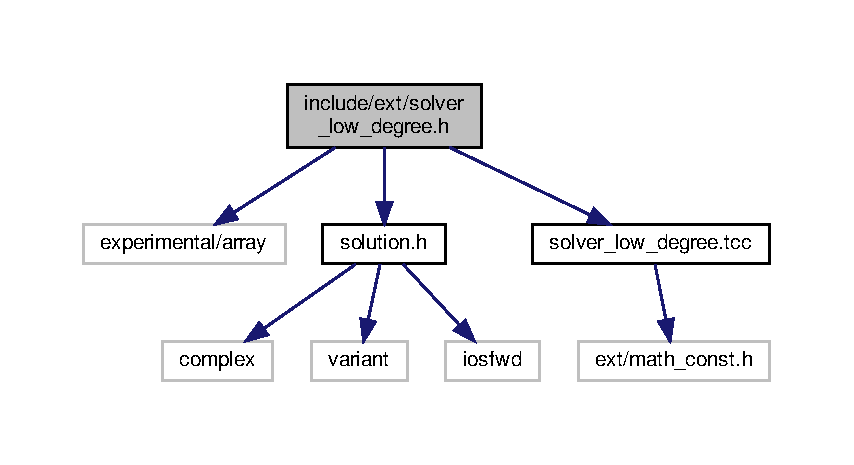
\includegraphics[width=350pt]{solver__low__degree_8h__incl}
\end{center}
\end{figure}
\subsection*{Namespaces}
\begin{DoxyCompactItemize}
\item 
 \hyperlink{namespace____gnu__cxx}{\+\_\+\+\_\+gnu\+\_\+cxx}
\end{DoxyCompactItemize}
\subsection*{Functions}
\begin{DoxyCompactItemize}
\item 
{\footnotesize template$<$typename \+\_\+\+Real , typename \+\_\+\+Iter $>$ }\\std\+::array$<$ solution\+\_\+t$<$ \+\_\+\+Real $>$, 3 $>$ \hyperlink{namespace____gnu__cxx_a422f638b186be2071012321de5f9bb48}{\+\_\+\+\_\+gnu\+\_\+cxx\+::\+\_\+\+\_\+cubic} (const \+\_\+\+Iter \&\+\_\+\+CC)
\begin{DoxyCompactList}\small\item\em Finds the roots of a cubic equation of the form\+: \[ a_3 x^3 + a_2 x^2 + a_1 x + a_0 = 0 \] for real coefficients $ a_k $. \end{DoxyCompactList}\item 
{\footnotesize template$<$typename \+\_\+\+Real $>$ }\\std\+::array$<$ solution\+\_\+t$<$ \+\_\+\+Real $>$, 3 $>$ \hyperlink{namespace____gnu__cxx_ad1ce809c9dd84dd6cd0229fb73f7dbec}{\+\_\+\+\_\+gnu\+\_\+cxx\+::\+\_\+\+\_\+cubic} (\+\_\+\+Real \+\_\+\+\_\+c0, \+\_\+\+Real \+\_\+\+\_\+c1, \+\_\+\+Real \+\_\+\+\_\+c2, \+\_\+\+Real \+\_\+\+\_\+c3)
\item 
{\footnotesize template$<$typename \+\_\+\+Real , typename \+\_\+\+Iter $>$ }\\std\+::array$<$ solution\+\_\+t$<$ \+\_\+\+Real $>$, 2 $>$ \hyperlink{namespace____gnu__cxx_aa8c3d98e6508a1e20a17c5980ccbbd99}{\+\_\+\+\_\+gnu\+\_\+cxx\+::\+\_\+\+\_\+quadratic} (const \+\_\+\+Iter \&\+\_\+\+CC)
\begin{DoxyCompactList}\small\item\em Finds the roots of a quadratic equation of the form\+: \[ a_2 x^2 + a_1 x + a_0 = 0 \] for real coefficients $ a_k $. \end{DoxyCompactList}\item 
{\footnotesize template$<$typename \+\_\+\+Real $>$ }\\std\+::array$<$ solution\+\_\+t$<$ \+\_\+\+Real $>$, 2 $>$ \hyperlink{namespace____gnu__cxx_af7f59d18caa0bf264f591103478ebcb2}{\+\_\+\+\_\+gnu\+\_\+cxx\+::\+\_\+\+\_\+quadratic} (\+\_\+\+Real \+\_\+\+\_\+c0, \+\_\+\+Real \+\_\+\+\_\+c1, \+\_\+\+Real \+\_\+\+\_\+c2)
\item 
{\footnotesize template$<$typename \+\_\+\+Real , typename \+\_\+\+Iter $>$ }\\std\+::array$<$ solution\+\_\+t$<$ \+\_\+\+Real $>$, 4 $>$ \hyperlink{namespace____gnu__cxx_ac813fbad739bf1d431845d5175f24701}{\+\_\+\+\_\+gnu\+\_\+cxx\+::\+\_\+\+\_\+quartic} (const \+\_\+\+Iter \&\+\_\+\+CC)
\begin{DoxyCompactList}\small\item\em Finds the roots a quartic equation of the form\+: \[ a_4 x^4 + a_3 x^3 + a_2 x^2 + a_1 x + a_0 = 0 \] for real coefficients $ a_k $. \end{DoxyCompactList}\item 
{\footnotesize template$<$typename \+\_\+\+Real $>$ }\\std\+::array$<$ solution\+\_\+t$<$ \+\_\+\+Real $>$, 4 $>$ \hyperlink{namespace____gnu__cxx_a6dbbccdfca9b8a8dffdf99432986f0c9}{\+\_\+\+\_\+gnu\+\_\+cxx\+::\+\_\+\+\_\+quartic} (\+\_\+\+Real \+\_\+\+\_\+c0, \+\_\+\+Real \+\_\+\+\_\+c1, \+\_\+\+Real \+\_\+\+\_\+c2, \+\_\+\+Real \+\_\+\+\_\+c3, \+\_\+\+Real \+\_\+\+\_\+c4)
\item 
{\footnotesize template$<$std\+::size\+\_\+t \+\_\+\+Dim, typename \+\_\+\+Iter , typename \+\_\+\+Num\+Tp $>$ }\\\+\_\+\+Num\+Tp \hyperlink{namespace____gnu__cxx_a957b92036746a66f3dff0c46cb18120b}{\+\_\+\+\_\+gnu\+\_\+cxx\+::\+\_\+\+\_\+refine\+\_\+solution\+\_\+halley} (\+\_\+\+Num\+Tp \+\_\+\+\_\+z, const \+\_\+\+Iter \&\+\_\+\+CC)
\item 
{\footnotesize template$<$std\+::size\+\_\+t \+\_\+\+Dim, typename \+\_\+\+Iter , typename \+\_\+\+Num\+Tp $>$ }\\\+\_\+\+Num\+Tp \hyperlink{namespace____gnu__cxx_a2b802e73df33cafb7f95800cbca6ff30}{\+\_\+\+\_\+gnu\+\_\+cxx\+::\+\_\+\+\_\+refine\+\_\+solution\+\_\+newton} (\+\_\+\+Num\+Tp \+\_\+\+\_\+z, const \+\_\+\+Iter \&\+\_\+\+CC)
\end{DoxyCompactItemize}


\subsection{Detailed Description}
This file is a G\+NU extension to the Standard C++ Library.

This file contains the declarations of free functions for solving quadratic, cubic, and quartic equations with real coefficients.

This file is a G\+NU extension to the Standard C++ Library.

This file contains the definitions of free functions for solving quadratic, cubic, and quartic equations with real coefficients. 
\hypertarget{solver__low__degree_8tcc}{}\section{include/ext/solver\+\_\+low\+\_\+degree.tcc File Reference}
\label{solver__low__degree_8tcc}\index{include/ext/solver\+\_\+low\+\_\+degree.\+tcc@{include/ext/solver\+\_\+low\+\_\+degree.\+tcc}}
{\ttfamily \#include $<$ext/math\+\_\+const.\+h$>$}\newline
Include dependency graph for solver\+\_\+low\+\_\+degree.\+tcc\+:
\nopagebreak
\begin{figure}[H]
\begin{center}
\leavevmode
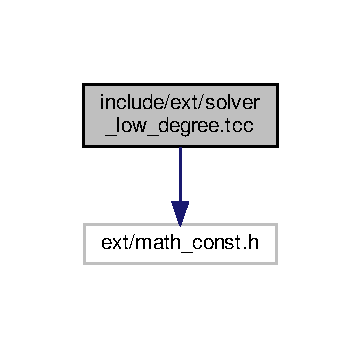
\includegraphics[width=173pt]{solver__low__degree_8tcc__incl}
\end{center}
\end{figure}
This graph shows which files directly or indirectly include this file\+:
\nopagebreak
\begin{figure}[H]
\begin{center}
\leavevmode
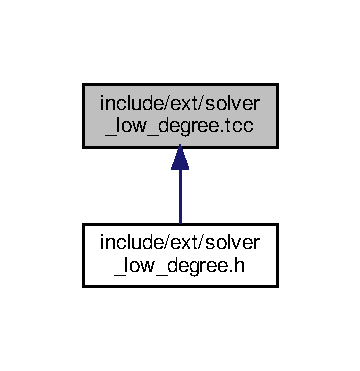
\includegraphics[width=173pt]{solver__low__degree_8tcc__dep__incl}
\end{center}
\end{figure}
\subsection*{Namespaces}
\begin{DoxyCompactItemize}
\item 
 \hyperlink{namespace____gnu__cxx}{\+\_\+\+\_\+gnu\+\_\+cxx}
\end{DoxyCompactItemize}
\subsection*{Macros}
\begin{DoxyCompactItemize}
\item 
\#define \hyperlink{solver__low__degree_8tcc_a10202d26918e17d656cf14da05e26477}{\+\_\+\+E\+X\+T\+\_\+\+S\+O\+L\+V\+E\+R\+\_\+\+L\+O\+W\+\_\+\+D\+E\+G\+R\+E\+E\+\_\+\+T\+CC}~1
\begin{DoxyCompactList}\small\item\em A guard for the low-\/degree polynomial solver functions header. \end{DoxyCompactList}\end{DoxyCompactItemize}
\subsection*{Functions}
\begin{DoxyCompactItemize}
\item 
{\footnotesize template$<$typename \+\_\+\+Real , typename \+\_\+\+Iter $>$ }\\std\+::array$<$ solution\+\_\+t$<$ \+\_\+\+Real $>$, 3 $>$ \hyperlink{namespace____gnu__cxx_a422f638b186be2071012321de5f9bb48}{\+\_\+\+\_\+gnu\+\_\+cxx\+::\+\_\+\+\_\+cubic} (const \+\_\+\+Iter \&\+\_\+\+CC)
\begin{DoxyCompactList}\small\item\em Finds the roots of a cubic equation of the form\+: \[ a_3 x^3 + a_2 x^2 + a_1 x + a_0 = 0 \] for real coefficients $ a_k $. \end{DoxyCompactList}\item 
{\footnotesize template$<$typename \+\_\+\+Real , typename \+\_\+\+Iter $>$ }\\std\+::array$<$ solution\+\_\+t$<$ \+\_\+\+Real $>$, 2 $>$ \hyperlink{namespace____gnu__cxx_aa8c3d98e6508a1e20a17c5980ccbbd99}{\+\_\+\+\_\+gnu\+\_\+cxx\+::\+\_\+\+\_\+quadratic} (const \+\_\+\+Iter \&\+\_\+\+CC)
\begin{DoxyCompactList}\small\item\em Finds the roots of a quadratic equation of the form\+: \[ a_2 x^2 + a_1 x + a_0 = 0 \] for real coefficients $ a_k $. \end{DoxyCompactList}\item 
{\footnotesize template$<$typename \+\_\+\+Real , typename \+\_\+\+Iter $>$ }\\std\+::array$<$ solution\+\_\+t$<$ \+\_\+\+Real $>$, 4 $>$ \hyperlink{namespace____gnu__cxx_ac813fbad739bf1d431845d5175f24701}{\+\_\+\+\_\+gnu\+\_\+cxx\+::\+\_\+\+\_\+quartic} (const \+\_\+\+Iter \&\+\_\+\+CC)
\begin{DoxyCompactList}\small\item\em Finds the roots a quartic equation of the form\+: \[ a_4 x^4 + a_3 x^3 + a_2 x^2 + a_1 x + a_0 = 0 \] for real coefficients $ a_k $. \end{DoxyCompactList}\item 
{\footnotesize template$<$std\+::size\+\_\+t \+\_\+\+Dim, typename \+\_\+\+Iter , typename \+\_\+\+Num\+Tp $>$ }\\\+\_\+\+Num\+Tp \hyperlink{namespace____gnu__cxx_a957b92036746a66f3dff0c46cb18120b}{\+\_\+\+\_\+gnu\+\_\+cxx\+::\+\_\+\+\_\+refine\+\_\+solution\+\_\+halley} (\+\_\+\+Num\+Tp \+\_\+\+\_\+z, const \+\_\+\+Iter \&\+\_\+\+CC)
\item 
{\footnotesize template$<$std\+::size\+\_\+t \+\_\+\+Dim, typename \+\_\+\+Iter , typename \+\_\+\+Num\+Tp $>$ }\\\+\_\+\+Num\+Tp \hyperlink{namespace____gnu__cxx_a2b802e73df33cafb7f95800cbca6ff30}{\+\_\+\+\_\+gnu\+\_\+cxx\+::\+\_\+\+\_\+refine\+\_\+solution\+\_\+newton} (\+\_\+\+Num\+Tp \+\_\+\+\_\+z, const \+\_\+\+Iter \&\+\_\+\+CC)
\item 
{\footnotesize template$<$std\+::size\+\_\+t \+\_\+\+Dim, typename \+\_\+\+Iter , typename \+\_\+\+Real $>$ }\\void \hyperlink{namespace____gnu__cxx_aa8dd4c7542667cc5a8e435ca53d6fad7}{\+\_\+\+\_\+gnu\+\_\+cxx\+::\+\_\+\+\_\+refine\+\_\+solutions} (std\+::array$<$ solution\+\_\+t$<$ \+\_\+\+Real $>$, \+\_\+\+Dim -\/ 1 $>$ \&\+\_\+\+ZZ, const \+\_\+\+Iter \&\+\_\+\+CC)
\end{DoxyCompactItemize}


\subsection{Macro Definition Documentation}
\mbox{\Hypertarget{solver__low__degree_8tcc_a10202d26918e17d656cf14da05e26477}\label{solver__low__degree_8tcc_a10202d26918e17d656cf14da05e26477}} 
\index{solver\+\_\+low\+\_\+degree.\+tcc@{solver\+\_\+low\+\_\+degree.\+tcc}!\+\_\+\+E\+X\+T\+\_\+\+S\+O\+L\+V\+E\+R\+\_\+\+L\+O\+W\+\_\+\+D\+E\+G\+R\+E\+E\+\_\+\+T\+CC@{\+\_\+\+E\+X\+T\+\_\+\+S\+O\+L\+V\+E\+R\+\_\+\+L\+O\+W\+\_\+\+D\+E\+G\+R\+E\+E\+\_\+\+T\+CC}}
\index{\+\_\+\+E\+X\+T\+\_\+\+S\+O\+L\+V\+E\+R\+\_\+\+L\+O\+W\+\_\+\+D\+E\+G\+R\+E\+E\+\_\+\+T\+CC@{\+\_\+\+E\+X\+T\+\_\+\+S\+O\+L\+V\+E\+R\+\_\+\+L\+O\+W\+\_\+\+D\+E\+G\+R\+E\+E\+\_\+\+T\+CC}!solver\+\_\+low\+\_\+degree.\+tcc@{solver\+\_\+low\+\_\+degree.\+tcc}}
\subsubsection{\texorpdfstring{\+\_\+\+E\+X\+T\+\_\+\+S\+O\+L\+V\+E\+R\+\_\+\+L\+O\+W\+\_\+\+D\+E\+G\+R\+E\+E\+\_\+\+T\+CC}{\_EXT\_SOLVER\_LOW\_DEGREE\_TCC}}
{\footnotesize\ttfamily \#define \+\_\+\+E\+X\+T\+\_\+\+S\+O\+L\+V\+E\+R\+\_\+\+L\+O\+W\+\_\+\+D\+E\+G\+R\+E\+E\+\_\+\+T\+CC~1}



A guard for the low-\/degree polynomial solver functions header. 



Definition at line 40 of file solver\+\_\+low\+\_\+degree.\+tcc.


\hypertarget{static__polynomial_8h}{}\section{include/ext/static\+\_\+polynomial.h File Reference}
\label{static__polynomial_8h}\index{include/ext/static\+\_\+polynomial.\+h@{include/ext/static\+\_\+polynomial.\+h}}
{\ttfamily \#include $<$limits$>$}\newline
{\ttfamily \#include $<$array$>$}\newline
{\ttfamily \#include $<$complex$>$}\newline
Include dependency graph for static\+\_\+polynomial.\+h\+:
\nopagebreak
\begin{figure}[H]
\begin{center}
\leavevmode
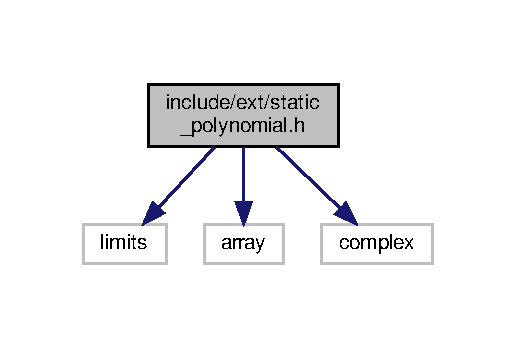
\includegraphics[width=248pt]{static__polynomial_8h__incl}
\end{center}
\end{figure}
\subsection*{Classes}
\begin{DoxyCompactItemize}
\item 
class \hyperlink{class____gnu__cxx_1_1__StaticPolynomial}{\+\_\+\+\_\+gnu\+\_\+cxx\+::\+\_\+\+Static\+Polynomial$<$ \+\_\+\+Tp, \+\_\+\+Num $>$}
\end{DoxyCompactItemize}
\subsection*{Namespaces}
\begin{DoxyCompactItemize}
\item 
 \hyperlink{namespace____gnu__cxx}{\+\_\+\+\_\+gnu\+\_\+cxx}
\end{DoxyCompactItemize}
\subsection*{Functions}
\begin{DoxyCompactItemize}
\item 
{\footnotesize template$<$typename \+\_\+\+Tp , std\+::size\+\_\+t \+\_\+\+NumA, std\+::size\+\_\+t \+\_\+\+NumB$>$ }\\bool \hyperlink{namespace____gnu__cxx_ad79bae6336788c58358fcf9fcd342cb9}{\+\_\+\+\_\+gnu\+\_\+cxx\+::operator!=} (const \+\_\+\+Static\+Polynomial$<$ \+\_\+\+Tp, \+\_\+\+NumA $>$ \&\+\_\+\+\_\+pa, const \+\_\+\+Static\+Polynomial$<$ \+\_\+\+Tp, \+\_\+\+NumB $>$ \&\+\_\+\+\_\+pb)
\item 
{\footnotesize template$<$typename \+\_\+\+Tp , std\+::size\+\_\+t \+\_\+\+Num$>$ }\\bool \hyperlink{namespace____gnu__cxx_a18cd3b1685ac1bb1c3f323e451e796d1}{\+\_\+\+\_\+gnu\+\_\+cxx\+::operator!=} (const \+\_\+\+Static\+Polynomial$<$ \+\_\+\+Tp, \+\_\+\+Num $>$ \&\+\_\+\+\_\+pa, const \+\_\+\+Static\+Polynomial$<$ \+\_\+\+Tp, \+\_\+\+Num $>$ \&\+\_\+\+\_\+pb)
\item 
{\footnotesize template$<$typename \+\_\+\+Tp , std\+::size\+\_\+t \+\_\+\+NumA, std\+::size\+\_\+t \+\_\+\+NumB$>$ }\\bool \hyperlink{namespace____gnu__cxx_a85c9740061a6497bb695d2ee147f52b8}{\+\_\+\+\_\+gnu\+\_\+cxx\+::operator==} (const \+\_\+\+Static\+Polynomial$<$ \+\_\+\+Tp, \+\_\+\+NumA $>$ \&, const \+\_\+\+Static\+Polynomial$<$ \+\_\+\+Tp, \+\_\+\+NumB $>$ \&)
\item 
{\footnotesize template$<$typename \+\_\+\+Tp , std\+::size\+\_\+t \+\_\+\+Num$>$ }\\bool \hyperlink{namespace____gnu__cxx_a2d1430ebbbaf156a6c80a8e8107960e1}{\+\_\+\+\_\+gnu\+\_\+cxx\+::operator==} (const \+\_\+\+Static\+Polynomial$<$ \+\_\+\+Tp, \+\_\+\+Num $>$ \&\+\_\+\+\_\+pa, const \+\_\+\+Static\+Polynomial$<$ \+\_\+\+Tp, \+\_\+\+Num $>$ \&\+\_\+\+\_\+pb)
\end{DoxyCompactItemize}


\subsection{Detailed Description}
Class definition for a static polynomial. 
%--- End generated contents ---

% Index
\backmatter
\newpage
\phantomsection
\clearemptydoublepage
\addcontentsline{toc}{chapter}{Index}
\printindex

\end{document}
